\newpage

%==================== Appendices ====================================================================
\cleardoublepage
\addcontentsline{toc}{section}{Appendices}
\appendix

% For large tables, use this just before the \begin{tabular}
%\resizebox{\linewidth}{!}{%

%==================== Appendix A ====================================================================
\renewcommand{\thefootnote}{\fnsymbol{footnote}}% Change the footnote style to lowercase letters
\addcontentsline{toc}{subsection}{Appendix A: Charter School \& Student Enrollment by State}
\section*{Appendix A\\Charter Schools \& Student Enrollment by State}
\label{appendixA}
\begin{center} \begin{singlespace}
\begin{longtable}{lrrrrrrr}
\caption[Charter schools \& student enrollment by state]{Charter schools \& student enrollment by state} \\
\thickline
      & Law     & \multicolumn{3}{c}{Totals for Charter Schools\tabfnm{b}}              & & \multicolumn{2}{c}{NAEP Students}\\
\cline{3-5} \cline{7-8}
State & Enacted & Operating & Closed & Students & & Charters & Publics\\
\hline
\endfirsthead
\multicolumn{8}{l}{Charter Schools \& Student Enrollment by State (cont.)}\\
\hline
      & Law     & \multicolumn{3}{c}{Totals for Charter Schools\tabfnm{b}}              & & \multicolumn{2}{c}{NAEP Students}\\
\cline{3-5} \cline{7-8}
State & Enacted & Operating & Closed & Students & & Charters & Publics\\
\hline
\endhead
\hline 
\endfoot
\thickline
\endlastfoot
Alabama\tabfnm{a}       &      & 0   & 0   & 0       & &   0 & 2759\\
Alaska                  & 1995 & 26  & 5   & 5,198   & &  69 & 2517\\
Arizona                 & 1994 & 510 & 96  & 119,903 & &  99 & 2674\\
Arkansas                & 1995 & 25  & 6   & 6,750   & &  30 & 2407\\
California              & 1992 & 802 & 103 & 316,468 & & 417 & 7803\\
Colorado                & 1993 & 151 & 10  & 54,497  & & 108 & 2598\\
Connecticut             & 1996 & 21  & 5   & 3,932   & &   0 & 2531\\
Delaware                & 1995 & 21  & 2   & 8,740   & & 180 & 2641\\
Washington DC           & 1996 & 93  & 16  & 25,385  & & 652 & 1336\\
Florida                 & 1996 & 382 & 82  & 108,382 & & 175 & 3876\\
Georgia                 & 1993 & 83  & 5   & 40,807  & &  64 & 3465\\
Hawaii                  & 1994 & 32  & 0   & 7,317   & & 132 & 2605\\
Idaho                   & 1998 & 32  & 1   & 10,492  & &  59 & 2784\\
Illinois                & 1996 & 74  & 8   & 27,683  & &  33 & 4015\\
Indiana                 & 2001 & 50  & 2   & 12,631  & &  11 & 2720\\
Iowa                    & 2002 & 10  & 0   & 1,462   & &   0 & 2839\\
Kansas                  & 1994 & 40  & 10  & 3,361   & &  17 & 2726\\
Kentucky\tabfnm{a}      &      & 0   & 0   & 0       & &   0 & 2696\\
Louisiana               & 1995 & 66  & 10  & 23,634  & &  97 & 2264\\
Maine\tabfnm{a}         &      & 0   & 0   & 0       & &   0 & 2658\\
Maryland                & 2003 & 34  & 2   & 7,301   & &   6 & 2825\\
Massachusetts           & 1993 & 64  & 6   & 23,905  & &  56 & 3667\\
Michigan                & 1993 & 250 & 27  & 94,092  & & 134 & 2480\\
Minnesota               & 1991 & 159 & 29  & 28,371  & &  16 & 2875\\
Mississippi             & 1997 & 1   & 0   & 367     & &   0 & 2613\\
Missouri                & 1998 & 39  & 5   & 13,125  & &  38 & 2771\\
Montana\tabfnm{a}       &      & 0   & 0   & 0       & &   0 & 2581\\
Nebraska\tabfnm{a}      &      & 0   & 0   & 0       & &   0 & 2688\\
Nevada                  & 1997 & 26  & 7   & 7,295   & &   0 & 2662\\
New Hampshire           & 1995 & 11  & 2   & 1,212   & &   0 & 2803\\
New Jersey              & 1996 & 64  & 19  & 17,986  & &   0 & 2813\\
New Mexico              & 1993 & 70  & 3   & 11,426  & &  54 & 2722\\
New York                & 1998 & 118 & 10  & 32,602  & &  16 & 3745\\
North Carolina          & 1996 & 103 & 32  & 30,445  & &  72 & 4090\\
North Dakota\tabfnm{a}  &      & 0   & 0   & 0       & &   0 & 2307\\
Ohio                    & 1997 & 293 & 48  & 94,171  & &  45 & 3746\\
Oklahoma                & 1999 & 14  & 1   & 4,770   & &   0 & 2612\\
Oregon                  & 1999 & 93  & 8   & 13,612  & &  41 & 2626\\
Pennsylvania            & 1997 & 133 & 12  & 61,823  & &  64 & 2709\\
Rhode Island            & 1995 & 11  & 0   & 2,894   & &  30 & 2621\\
South Carolina          & 1996 & 36  & 10  & 8,705   & &  16 & 2697\\
South Dakota\tabfnm{a}  &      & 0   & 0   & 0       & &   0 & 2889\\
Tennessee               & 2002 & 14  & 1   & 2,585   & &  54 & 2815\\
Texas                   & 1995 & 331 & 33  & 108,541 & & 199 & 7070\\
Utah                    & 1998 & 68  & 1   & 23,233  & &  38 & 2722\\
Vermont\tabfnm{a}       &      & 0   & 0   & 0       & &   0 & 2003\\
Virginia                & 1998 & 4   & 3   & 275     & &   0 & 2848\\
Washington\tabfnm{a}    &      & 0   & 0   & 0       & &   0 & 2968\\
West Virginia\tabfnm{a} &      & 0   & 0   & 0       & &   0 & 2831\\
Wisconsin               & 1993 & 221 & 37  & 41,799  & & 114 & 2592\\
Wyoming                 & 1995 & 3   & 0   & 244     & &   0 & 1897\\
\hline
Total                   &      & 4,578 & 657 & 1,407,421 & & 3,164 & 156,963 \\
\end{longtable}
\tabfnt{a}{State currently does not have a charter school law.}
\tabfnt{b}{Source: \citeA{cernumbers}}
\end{singlespace} \end{center}
\renewcommand{\thefootnote}{\arabic{footnote}}% Reset the footnotes back to numbers


%==================== Appendix B ====================================================================
\newpage
\addcontentsline{toc}{subsection}{Appendix B: Descriptive Statistics}
\section*{Appendix B\\Descriptive Statistics}
\label{appendixB}

\begin{singlespace}

\input{../Tables2009/g4Math-desc.tex}
% latex table generated in R 3.0.0 by xtable 1.7-1 package
% Fri May 31 15:00:30 2013
\begin{sidewaystable}[ht]
\centering
\caption{Grade 4 Math Unadjusted NAEP Score} 
\label{tab:g4math-unadjscore}
\begin{tabular}{lrrrrrr@{\extracolsep{10pt}}rrrrrr}
  \hline & \multicolumn{6}{c}{Charter Schools} & \multicolumn{6}{c}{Public Schools} \\ \cline{2-7} \cline{8-13} & n & mean & sd & median & min & max & n & mean & sd & median & min & max \\ 
  \hline
Overall & 3625 & 231.93 & 28.19 & 232.18 & 136.95 & 310.45 & 159338 & 238.34 & 27.71 & 239.71 & 117.69 & 334.07 \\ 
  Alaska & 102 & 247.41 & 24.64 & 248.79 & 183.80 & 296.82 & 2496 & 238.50 & 28.87 & 240.91 & 133.70 & 314.90 \\ 
  Arkansas & 226 & 229.38 & 29.27 & 230.22 & 145.74 & 294.08 & 2836 & 228.66 & 29.47 & 229.71 & 142.09 & 324.86 \\ 
  Canal zone & 170 & 223.41 & 26.86 & 221.21 & 152.40 & 290.14 & 7241 & 227.05 & 30.42 & 227.52 & 127.08 & 330.95 \\ 
  Connecticut & 132 & 250.45 & 28.67 & 256.63 & 148.19 & 308.90 & 2550 & 242.34 & 28.39 & 244.89 & 130.83 & 317.99 \\ 
  D.C. & 512 & 217.48 & 26.97 & 215.26 & 146.95 & 306.62 & 1282 & 219.99 & 32.15 & 219.20 & 133.26 & 317.28 \\ 
  Florida & 195 & 240.20 & 26.34 & 238.76 & 168.45 & 294.30 & 2586 & 239.42 & 24.64 & 239.68 & 159.44 & 316.57 \\ 
  Idaho & 166 & 241.09 & 24.28 & 244.36 & 175.09 & 293.17 & 4531 & 239.76 & 24.97 & 240.17 & 147.51 & 324.61 \\ 
  Illinois & 164 & 241.86 & 25.56 & 244.89 & 183.18 & 310.45 & 3865 & 232.69 & 28.18 & 232.54 & 140.58 & 316.17 \\ 
  Iowa &  57 & 230.95 & 26.26 & 234.88 & 146.85 & 273.46 & 2695 & 236.28 & 31.24 & 239.72 & 127.32 & 314.05 \\ 
  Kansas &  60 & 255.08 & 20.79 & 255.56 & 183.42 & 300.83 & 3024 & 240.97 & 24.84 & 242.25 & 139.84 & 314.77 \\ 
  Kentucky &  78 & 229.74 & 27.71 & 231.49 & 147.64 & 295.55 & 4059 & 232.94 & 29.83 & 233.75 & 117.69 & 318.75 \\ 
  Michigan &  65 & 230.80 & 16.68 & 230.98 & 197.30 & 279.19 & 2830 & 229.16 & 24.90 & 229.32 & 144.26 & 308.71 \\ 
  Mississippi & 141 & 219.12 & 26.52 & 217.25 & 164.93 & 293.18 & 3249 & 239.22 & 27.40 & 238.06 & 148.45 & 318.09 \\ 
  Missouri &  52 & 229.29 & 22.62 & 226.30 & 179.65 & 284.75 & 3615 & 248.36 & 25.63 & 249.08 & 145.76 & 317.96 \\ 
  Montana & 215 & 218.06 & 29.43 & 216.04 & 136.95 & 288.98 & 3204 & 229.38 & 31.66 & 231.15 & 128.36 & 318.70 \\ 
  Nebraska & 109 & 247.68 & 26.51 & 248.08 & 188.30 & 302.32 & 3204 & 248.59 & 27.03 & 251.09 & 150.58 & 323.00 \\ 
  New York &  72 & 231.01 & 31.20 & 229.16 & 162.07 & 303.29 & 2977 & 234.90 & 25.81 & 236.10 & 137.78 & 303.75 \\ 
  North Dakota &  74 & 224.15 & 23.57 & 223.48 & 179.04 & 284.71 & 2780 & 247.30 & 26.13 & 249.06 & 155.28 & 325.63 \\ 
  Oklahoma &  60 & 229.73 & 21.88 & 230.70 & 189.84 & 269.90 & 3997 & 239.50 & 26.83 & 240.45 & 145.65 & 315.10 \\ 
  Oregon &  96 & 249.72 & 19.40 & 250.68 & 206.39 & 290.68 & 4320 & 243.07 & 26.92 & 243.12 & 130.47 & 323.33 \\ 
  Rhode Island & 124 & 218.15 & 22.02 & 217.22 & 159.99 & 269.17 & 3324 & 237.62 & 29.58 & 239.43 & 126.61 & 319.60 \\ 
  Utah &  79 & 230.94 & 23.07 & 227.57 & 185.38 & 297.38 & 2404 & 239.08 & 28.41 & 241.89 & 136.10 & 307.88 \\ 
  Washington &  91 & 231.23 & 20.75 & 229.44 & 166.83 & 278.23 & 6193 & 238.97 & 24.48 & 239.19 & 139.25 & 317.06 \\ 
  West Virginia & 197 & 247.20 & 25.79 & 250.06 & 164.01 & 305.53 & 3145 & 239.22 & 28.47 & 241.50 & 130.38 & 319.46 \\ 
  DoDEA/DDESS & 136 & 229.43 & 26.14 & 226.78 & 178.41 & 289.56 & 3694 & 237.95 & 29.14 & 239.24 & 134.42 & 320.51 \\ 
   \hline
\end{tabular}
\end{sidewaystable}
 \clearpage

% latex table generated in R 3.0.1 by xtable 1.7-1 package
% Wed Jun 19 20:22:03 2013
\begin{longtable}{lrr@{\extracolsep{10pt}}rr}
\caption{Grade 4 Reading Descriptive Statistics} \\ 
   \thickline & \multicolumn{2}{c}{Traditional} & \multicolumn{2}{c}{Charter} \\  \endfirsthead \multicolumn{5}{l}{{...continued from previous page}}\\ \hline & \multicolumn{2}{c}{Charter} & \multicolumn{2}{c}{Traditional}  \\ \hline \endhead \thickline \multicolumn{5}{r}{continued on next page...} \\ \endfoot \multicolumn{5}{c}{} \\ \endlastfoot  \pagebreak[2] \hline \multicolumn{5}{c}{Race/ethnicity from school records (raw data)} \\ \cline{1-5} White & 96992 & 58\% & 1343 & 34\% \\ 
  Black & 29127 & 17\% & 1636 & 42\% \\ 
  Hispanic & 28133 & 17\% & 705 & 18\% \\ 
  Asian Amer/Pacif Is & 8114 & 5\% & 162 & 4\% \\ 
  Amer Ind/Alaska Nat & 3898 & 2\% &  49 & 1\% \\ 
  Other & 2333 & 1\% &  41 & 1\% \\ 
  Unknown &   0 & 0\% &   0 & 0\% \\ 
   \pagebreak[2] \hline \multicolumn{5}{c}{Natl School Lunch Prog eligibility (3 categories)} \\ \cline{1-5} Eligible & 82354 & 49\% & 2223 & 56\% \\ 
  Not eligible & 85304 & 51\% & 1528 & 39\% \\ 
  Info not available & 939 & 1\% & 185 & 5\% \\ 
  Unknown &   0 & 0\% &   0 & 0\% \\ 
   \pagebreak[2] \hline \multicolumn{5}{c}{Student has Individualized Education Plan} \\ \cline{1-5} Yes, IEP & 16579 & 10\% & 307 & 8\% \\ 
  Yes, 504 plan & 1385 & 1\% &  29 & 1\% \\ 
  Yes, 504 in process &   0 & 0\% &   0 & 0\% \\ 
  Not IEP & 150596 & 89\% & 3600 & 91\% \\ 
  Omitted &   0 & 0\% &   0 & 0\% \\ 
  Unknown &  37 & 0\% &   0 & 0\% \\ 
   \pagebreak[2] \hline \multicolumn{5}{c}{Student classified Eng Lang Learner (3 categories)} \\ \cline{1-5} Yes & 12095 & 7\% & 285 & 7\% \\ 
  No & 153110 & 91\% & 3569 & 91\% \\ 
  Formerly ELL & 3357 & 2\% &  82 & 2\% \\ 
  Omitted &   0 & 0\% &   0 & 0\% \\ 
  Unknown &  35 & 0\% &   0 & 0\% \\ 
   \pagebreak[2] \hline \multicolumn{5}{c}{Gender} \\ \cline{1-5} Male & 85214 & 51\% & 1960 & 50\% \\ 
  Female & 83383 & 49\% & 1976 & 50\% \\ 
  Unknown &   0 & 0\% &   0 & 0\% \\ 
   \pagebreak[2] \hline \multicolumn{5}{c}{Student classified as having a disability (504)} \\ \cline{1-5} Student with disabi & 17964 & 11\% & 336 & 9\% \\ 
  Not student with di & 150596 & 89\% & 3600 & 91\% \\ 
  Omitted &  37 & 0\% &   0 & 0\% \\ 
  Unknown &   0 & 0\% &   0 & 0\% \\ 
   \pagebreak[2] \hline \multicolumn{5}{c}{Student classified SD or ELL} \\ \cline{1-5} Student with disabi & 16722 & 10\% & 314 & 8\% \\ 
  English language le & 10853 & 6\% & 263 & 7\% \\ 
  Both SD and ELL & 1242 & 1\% &  22 & 1\% \\ 
  Neither SD nor ELL & 139727 & 83\% & 3337 & 85\% \\ 
  Unknown &  53 & 0\% &   0 & 0\% \\ 
   \pagebreak[2] \hline \multicolumn{5}{c}{Newspaper in home} \\ \cline{1-5} Yes & 47839 & 28\% & 1141 & 29\% \\ 
  No & 59247 & 35\% & 1327 & 34\% \\ 
  I Don't Know & 58294 & 35\% & 1343 & 34\% \\ 
  Omitted & 3205 & 2\% & 125 & 3\% \\ 
  Multiple &  12 & 0\% &   0 & 0\% \\ 
  Unknown &   0 & 0\% &   0 & 0\% \\ 
   \pagebreak[2] \hline \multicolumn{5}{c}{Magazines in home} \\ \cline{1-5} Yes & 95695 & 57\% & 2225 & 57\% \\ 
  No & 40167 & 24\% & 911 & 23\% \\ 
  I Don't Know & 29309 & 17\% & 667 & 17\% \\ 
  Omitted & 3404 & 2\% & 133 & 3\% \\ 
  Multiple &  22 & 0\% &   0 & 0\% \\ 
  Unknown &   0 & 0\% &   0 & 0\% \\ 
   \pagebreak[2] \hline \multicolumn{5}{c}{Books in home} \\ \cline{1-5} 0-10 books & 19634 & 12\% & 434 & 11\% \\ 
  11-25 books & 35306 & 21\% & 901 & 23\% \\ 
  26-100 books & 56725 & 34\% & 1217 & 31\% \\ 
  More than 100 books & 53526 & 32\% & 1258 & 32\% \\ 
  Omitted & 3359 & 2\% & 126 & 3\% \\ 
  Multiple &  47 & 0\% &   0 & 0\% \\ 
  Unknown &   0 & 0\% &   0 & 0\% \\ 
   \pagebreak[2] \hline \multicolumn{5}{c}{Computer in home} \\ \cline{1-5} Yes & 144162 & 86\% & 3362 & 85\% \\ 
  No & 20419 & 12\% & 428 & 11\% \\ 
  Omitted & 3999 & 2\% & 146 & 4\% \\ 
  Multiple &  17 & 0\% &   0 & 0\% \\ 
  Unknown &   0 & 0\% &   0 & 0\% \\ 
   \pagebreak[2] \hline \multicolumn{5}{c}{Encyclopedia in home} \\ \cline{1-5} Yes & 85818 & 51\% & 2035 & 52\% \\ 
  No & 25320 & 15\% & 544 & 14\% \\ 
  I Don't Know & 54087 & 32\% & 1229 & 31\% \\ 
  Omitted & 3350 & 2\% & 128 & 3\% \\ 
  Multiple &  22 & 0\% &   0 & 0\% \\ 
  Unknown &   0 & 0\% &   0 & 0\% \\ 
   \pagebreak[2] \hline \multicolumn{5}{c}{Pages read in school and for homework} \\ \cline{1-5} 5 or fewer & 34944 & 21\% & 912 & 23\% \\ 
  6-10 & 30880 & 18\% & 746 & 19\% \\ 
  11-15 & 23139 & 14\% & 449 & 11\% \\ 
  16-20 & 23805 & 14\% & 529 & 13\% \\ 
  More than 20 & 52313 & 31\% & 1167 & 30\% \\ 
  Omitted & 3450 & 2\% & 129 & 3\% \\ 
  Multiple &  66 & 0\% &   4 & 0\% \\ 
  Unknown &   0 & 0\% &   0 & 0\% \\ 
   \pagebreak[2] \hline \multicolumn{5}{c}{Talk about studies at home} \\ \cline{1-5} Never or hardly eve & 29602 & 18\% & 648 & 16\% \\ 
  Every few weeks & 22498 & 13\% & 475 & 12\% \\ 
  About once a week & 19884 & 12\% & 429 & 11\% \\ 
  2-3 times a week & 33893 & 20\% & 687 & 17\% \\ 
  Every day & 59212 & 35\% & 1566 & 40\% \\ 
  Omitted & 3465 & 2\% & 129 & 3\% \\ 
  Multiple &  43 & 0\% &   2 & 0\% \\ 
  Unknown &   0 & 0\% &   0 & 0\% \\ 
   \pagebreak[2] \hline \multicolumn{5}{c}{Days absent from school last month} \\ \cline{1-5} None & 84418 & 50\% & 1838 & 47\% \\ 
  1-2 days & 49650 & 29\% & 1177 & 30\% \\ 
  3-4 days & 19327 & 11\% & 474 & 12\% \\ 
  5-10 days & 7608 & 5\% & 208 & 5\% \\ 
  More than 10 days & 4136 & 2\% & 109 & 3\% \\ 
  Omitted & 3396 & 2\% & 128 & 3\% \\ 
  Multiple &  62 & 0\% &   2 & 0\% \\ 
  Unknown &   0 & 0\% &   0 & 0\% \\ 
   \pagebreak[2] \hline \multicolumn{5}{c}{Language other than English spoken in home} \\ \cline{1-5} Never & 90390 & 54\% & 1798 & 46\% \\ 
  Once in a while & 36078 & 21\% & 901 & 23\% \\ 
  Half the time & 12161 & 7\% & 362 & 9\% \\ 
  All or most of time & 26507 & 16\% & 743 & 19\% \\ 
  Omitted & 3412 & 2\% & 129 & 3\% \\ 
  Multiple &  49 & 0\% &   3 & 0\% \\ 
  Unknown &   0 & 0\% &   0 & 0\% \\ 
   \pagebreak[2] \hline \multicolumn{5}{c}{Learn a lot when reading books} \\ \cline{1-5} Never or hardly eve & 8448 & 5\% & 185 & 5\% \\ 
  Sometimes & 59897 & 36\% & 1331 & 34\% \\ 
  Often & 50052 & 30\% & 1076 & 27\% \\ 
  Always or almost & 46493 & 28\% & 1201 & 31\% \\ 
  Omitted & 3687 & 2\% & 142 & 4\% \\ 
  Multiple &  20 & 0\% &   1 & 0\% \\ 
  Unknown &   0 & 0\% &   0 & 0\% \\ 
   \pagebreak[2] \hline \multicolumn{5}{c}{Reading is a favorite subject} \\ \cline{1-5} Never or hardly eve & 25581 & 15\% & 611 & 16\% \\ 
  Sometimes & 60476 & 36\% & 1409 & 36\% \\ 
  Often & 36703 & 22\% & 783 & 20\% \\ 
  Always or almost & 41959 & 25\% & 987 & 25\% \\ 
  Omitted & 3855 & 2\% & 146 & 4\% \\ 
  Multiple &  23 & 0\% &   0 & 0\% \\ 
  Unknown &   0 & 0\% &   0 & 0\% \\ 
   \pagebreak[2] \hline \multicolumn{5}{c}{Do reading at after-school or tutoring program} \\ \cline{1-5} Yes & 60364 & 36\% & 1718 & 44\% \\ 
  No & 102803 & 61\% & 2029 & 52\% \\ 
  Omitted & 5387 & 3\% & 189 & 5\% \\ 
  Multiple &  43 & 0\% &   0 & 0\% \\ 
  Unknown &   0 & 0\% &   0 & 0\% \\ 
   \pagebreak[2] \hline \multicolumn{5}{c}{Go to book clubs, competitions, fairs for reading} \\ \cline{1-5} Yes & 49006 & 29\% & 1255 & 32\% \\ 
  No & 113968 & 68\% & 2491 & 63\% \\ 
  Omitted & 5592 & 3\% & 189 & 5\% \\ 
  Multiple &  31 & 0\% &   1 & 0\% \\ 
  Unknown &   0 & 0\% &   0 & 0\% \\ 
   \pagebreak[2] \hline \multicolumn{5}{c}{Read for fun on own} \\ \cline{1-5} Never or hardly eve & 25028 & 15\% & 584 & 15\% \\ 
  Once or twice/month & 24696 & 15\% & 569 & 14\% \\ 
  1-2 times a week & 41186 & 24\% & 923 & 23\% \\ 
  Almost every day & 72670 & 43\% & 1677 & 43\% \\ 
  Omitted & 4984 & 3\% & 182 & 5\% \\ 
  Multiple &  33 & 0\% &   1 & 0\% \\ 
  Unknown &   0 & 0\% &   0 & 0\% \\ 
   \pagebreak[2] \hline \multicolumn{5}{c}{Talk with friends about what you read} \\ \cline{1-5} Never or hardly eve & 46333 & 27\% & 997 & 25\% \\ 
  Once or twice/month & 34554 & 20\% & 739 & 19\% \\ 
  1-2 times a week & 43383 & 26\% & 943 & 24\% \\ 
  Almost every day & 40113 & 24\% & 1106 & 28\% \\ 
  Omitted & 4180 & 2\% & 150 & 4\% \\ 
  Multiple &  34 & 0\% &   1 & 0\% \\ 
  Unknown &   0 & 0\% &   0 & 0\% \\ 
   \pagebreak[2] \hline \multicolumn{5}{c}{Read a book you chose yourself} \\ \cline{1-5} Never or hardly eve & 22712 & 13\% & 593 & 15\% \\ 
  Sometimes & 40804 & 24\% & 1009 & 26\% \\ 
  Often & 42467 & 25\% & 932 & 24\% \\ 
  Always or almost & 56171 & 33\% & 1196 & 30\% \\ 
  Omitted & 6413 & 4\% & 205 & 5\% \\ 
  Multiple &  30 & 0\% &   1 & 0\% \\ 
  Unknown &   0 & 0\% &   0 & 0\% \\ 
  \hline
\label{tab:g4Reading-desc}
\end{longtable}

% latex table generated in R 3.0.0 by xtable 1.7-1 package
% Fri May 31 15:00:31 2013
\begin{sidewaystable}[ht]
\centering
\caption{Grade 4 Reading Unadjusted NAEP Score} 
\label{tab:g4read-unadjscore}
\begin{tabular}{lrrrrrr@{\extracolsep{10pt}}rrrrrr}
  \hline & \multicolumn{6}{c}{Charter Schools} & \multicolumn{6}{c}{Public Schools} \\ \cline{2-7} \cline{8-13} & n & mean & sd & median & min & max & n & mean & sd & median & min & max \\ 
  \hline
Overall & 3936 & 213.26 & 32.94 & 215.22 & 92.27 & 302.97 & 168597 & 218.76 & 33.66 & 221.79 & 14.71 & 330.96 \\ 
  Alaska & 117 & 226.06 & 33.86 & 233.08 & 101.93 & 278.72 & 2666 & 214.43 & 36.60 & 219.70 & 78.50 & 302.46 \\ 
  Arkansas & 242 & 213.15 & 34.22 & 216.30 & 105.63 & 294.52 & 2943 & 208.58 & 38.27 & 212.92 & 14.71 & 319.32 \\ 
  Canal zone & 183 & 196.96 & 35.30 & 194.82 & 92.27 & 286.62 & 7822 & 204.44 & 35.95 & 206.11 & 51.07 & 318.34 \\ 
  Connecticut & 143 & 229.69 & 33.61 & 235.33 & 124.55 & 291.85 & 2777 & 225.49 & 34.52 & 230.29 & 85.98 & 316.87 \\ 
  D.C. & 541 & 198.75 & 31.53 & 199.60 & 102.07 & 280.99 & 1307 & 204.14 & 37.69 & 203.42 & 71.14 & 330.96 \\ 
  Florida & 216 & 222.89 & 27.69 & 223.23 & 152.52 & 293.06 & 2649 & 225.96 & 27.61 & 227.81 & 113.17 & 309.18 \\ 
  Idaho & 185 & 227.25 & 24.58 & 228.11 & 141.86 & 288.14 & 4771 & 224.10 & 29.65 & 226.17 & 97.23 & 312.59 \\ 
  Illinois & 179 & 220.16 & 32.54 & 220.82 & 94.63 & 287.95 & 4056 & 215.07 & 33.27 & 216.54 & 89.20 & 321.26 \\ 
  Iowa &  78 & 215.14 & 36.63 & 222.41 & 96.15 & 289.85 & 2914 & 210.77 & 38.37 & 214.86 & 50.22 & 309.30 \\ 
  Kansas &  72 & 242.29 & 27.73 & 247.02 & 157.89 & 290.30 & 3169 & 220.49 & 31.59 & 224.11 & 73.45 & 294.68 \\ 
  Kentucky &  81 & 204.56 & 33.03 & 206.21 & 134.27 & 276.43 & 4314 & 213.09 & 36.59 & 216.16 & 82.70 & 322.40 \\ 
  Michigan &  73 & 200.08 & 24.97 & 197.83 & 158.07 & 269.88 & 3079 & 207.87 & 31.56 & 209.30 & 75.54 & 298.16 \\ 
  Mississippi & 152 & 207.05 & 28.29 & 208.95 & 142.04 & 274.30 & 3297 & 220.71 & 32.60 & 220.73 & 109.43 & 322.77 \\ 
  Missouri &  54 & 225.77 & 22.09 & 225.23 & 169.00 & 265.05 & 3894 & 229.30 & 30.48 & 231.56 & 95.48 & 309.48 \\ 
  Montana & 217 & 201.20 & 31.78 & 202.59 & 123.87 & 289.31 & 3487 & 212.74 & 34.23 & 215.29 & 75.67 & 302.63 \\ 
  Nebraska & 109 & 221.06 & 36.91 & 223.34 & 101.89 & 285.11 & 3506 & 222.79 & 34.75 & 227.05 & 58.17 & 316.17 \\ 
  New York &  75 & 215.17 & 29.94 & 216.60 & 134.65 & 278.63 & 3155 & 210.12 & 35.62 & 213.99 & 18.03 & 295.53 \\ 
  North Dakota &  80 & 213.75 & 21.85 & 212.65 & 153.51 & 263.03 & 2805 & 230.06 & 28.90 & 231.41 & 118.16 & 321.05 \\ 
  Oklahoma &  69 & 220.92 & 30.41 & 218.55 & 157.69 & 300.34 & 4162 & 221.95 & 32.22 & 224.25 & 99.34 & 306.82 \\ 
  Oregon & 104 & 226.53 & 26.97 & 227.31 & 148.58 & 287.27 & 4720 & 219.46 & 34.73 & 223.00 & 40.55 & 309.55 \\ 
  Rhode Island & 138 & 196.41 & 31.14 & 196.45 & 112.19 & 273.31 & 3464 & 218.63 & 32.97 & 220.65 & 101.22 & 305.91 \\ 
  South Dakota &  56 & 225.22 & 31.87 & 229.31 & 148.54 & 285.83 & 3027 & 217.79 & 35.12 & 221.68 & 44.79 & 306.49 \\ 
  Tennessee &  59 & 218.66 & 33.26 & 221.67 & 130.12 & 302.97 & 3846 & 216.38 & 36.39 & 218.94 & 45.75 & 316.07 \\ 
  Utah &  85 & 217.99 & 31.30 & 218.14 & 135.33 & 283.96 & 2566 & 222.83 & 34.75 & 226.45 & 49.36 & 310.49 \\ 
  Washington & 100 & 217.52 & 24.77 & 220.63 & 151.32 & 277.02 & 5854 & 216.69 & 30.85 & 216.91 & 91.15 & 318.03 \\ 
  West Virginia & 203 & 228.59 & 27.26 & 231.71 & 137.46 & 287.80 & 3290 & 218.54 & 32.67 & 222.79 & 46.89 & 303.80 \\ 
  DoDEA/DDESS & 153 & 200.04 & 32.60 & 198.92 & 123.03 & 273.93 & 3935 & 214.63 & 35.37 & 218.79 & 92.04 & 301.72 \\ 
   \hline
\end{tabular}
\end{sidewaystable}
 \clearpage

% latex table generated in R 3.0.1 by xtable 1.7-1 package
% Wed Jun 19 20:22:07 2013
{\normalsize
\begin{longtable}{lrr@{\extracolsep{10pt}}rr}
\caption{Grade 8 math descriptive statistics} \\ 
   \thickline & \multicolumn{2}{c}{Traditional} & \multicolumn{2}{c}{Charter} \\  \endfirsthead \multicolumn{5}{l}{{...continued from previous page}}\\ \hline & \multicolumn{2}{c}{Charter} & \multicolumn{2}{c}{Traditional}  \\ \hline \endhead \thickline \multicolumn{5}{r}{continued on next page...} \\ \endfoot \multicolumn{5}{c}{} \\ \endlastfoot  \pagebreak[2] \hline \multicolumn{5}{c}{Race/ethnicity from school records (raw data)} \\ \cline{1-5} White & 89701 & 59\% & 1114 & 27\% \\ 
  Black & 26613 & 18\% & 1711 & 41\% \\ 
  Hispanic & 23669 & 16\% & 974 & 24\% \\ 
  Asian Amer/Pacif Is & 7318 & 5\% & 230 & 6\% \\ 
  Amer Ind/Alaska Nat & 3250 & 2\% &  55 & 1\% \\ 
  Other & 1497 & 1\% &  46 & 1\% \\ 
  Unknown &   0 & 0\% &   0 & 0\% \\ 
   \pagebreak[2] \hline \multicolumn{5}{c}{Natl School Lunch Prog eligibility (3 categories)} \\ \cline{1-5} Eligible & 67525 & 44\% & 2358 & 57\% \\ 
  Not eligible & 83452 & 55\% & 1553 & 38\% \\ 
  Info not available & 1071 & 1\% & 219 & 5\% \\ 
  Unknown &   0 & 0\% &   0 & 0\% \\ 
   \pagebreak[2] \hline \multicolumn{5}{c}{Student has Individualized Education Plan} \\ \cline{1-5} Yes, IEP & 14792 & 10\% & 377 & 9\% \\ 
  Yes, 504 plan & 1308 & 1\% &  38 & 1\% \\ 
  Yes, 504 in process &   0 & 0\% &   0 & 0\% \\ 
  Not IEP & 135935 & 89\% & 3715 & 90\% \\ 
  Unknown &  13 & 0\% &   0 & 0\% \\ 
   \pagebreak[2] \hline \multicolumn{5}{c}{Student classified Eng Lang Learner (3 categories)} \\ \cline{1-5} Yes & 6615 & 4\% & 276 & 7\% \\ 
  No & 142006 & 93\% & 3712 & 90\% \\ 
  Formerly ELL & 3404 & 2\% & 140 & 3\% \\ 
  Unknown &  23 & 0\% &   2 & 0\% \\ 
   \pagebreak[2] \hline \multicolumn{5}{c}{Gender} \\ \cline{1-5} Male & 76976 & 51\% & 1996 & 48\% \\ 
  Female & 75072 & 49\% & 2134 & 52\% \\ 
  Unknown &   0 & 0\% &   0 & 0\% \\ 
   \pagebreak[2] \hline \multicolumn{5}{c}{Student classified as having a disability (504)} \\ \cline{1-5} Student with disabi & 16100 & 11\% & 415 & 10\% \\ 
  Not student with di & 135935 & 89\% & 3715 & 90\% \\ 
  Omitted &  13 & 0\% &   0 & 0\% \\ 
  Unknown &   0 & 0\% &   0 & 0\% \\ 
   \pagebreak[2] \hline \multicolumn{5}{c}{Student classified SD or ELL} \\ \cline{1-5} Student with disabi & 15250 & 10\% & 389 & 9\% \\ 
  English language le & 5765 & 4\% & 250 & 6\% \\ 
  Both SD and ELL & 850 & 1\% &  26 & 1\% \\ 
  Neither SD nor ELL & 130158 & 86\% & 3464 & 84\% \\ 
  Unknown &  25 & 0\% &   1 & 0\% \\ 
   \pagebreak[2] \hline \multicolumn{5}{c}{Newspaper in home} \\ \cline{1-5} Yes & 55041 & 36\% & 1501 & 36\% \\ 
  No & 62855 & 41\% & 1740 & 42\% \\ 
  I Don't Know & 31056 & 20\% & 862 & 21\% \\ 
  Omitted & 3068 & 2\% &  27 & 1\% \\ 
  Multiple &  28 & 0\% &   0 & 0\% \\ 
  Unknown &   0 & 0\% &   0 & 0\% \\ 
   \pagebreak[2] \hline \multicolumn{5}{c}{Magazines in home} \\ \cline{1-5} Yes & 92419 & 61\% & 2444 & 59\% \\ 
  No & 40632 & 27\% & 1198 & 29\% \\ 
  I Don't Know & 15801 & 10\% & 456 & 11\% \\ 
  Omitted & 3172 & 2\% &  32 & 1\% \\ 
  Multiple &  24 & 0\% &   0 & 0\% \\ 
  Unknown &   0 & 0\% &   0 & 0\% \\ 
   \pagebreak[2] \hline \multicolumn{5}{c}{Books in home} \\ \cline{1-5} 0-10 books & 21803 & 14\% & 578 & 14\% \\ 
  11-25 books & 32216 & 21\% & 966 & 23\% \\ 
  26-100 books & 51674 & 34\% & 1404 & 34\% \\ 
  More than 100 books & 42985 & 28\% & 1148 & 28\% \\ 
  Omitted & 3318 & 2\% &  34 & 1\% \\ 
  Multiple &  52 & 0\% &   0 & 0\% \\ 
  Unknown &   0 & 0\% &   0 & 0\% \\ 
   \pagebreak[2] \hline \multicolumn{5}{c}{Computer in home} \\ \cline{1-5} Yes & 133737 & 88\% & 3658 & 89\% \\ 
  No & 13012 & 9\% & 386 & 9\% \\ 
  Omitted & 5276 & 3\% &  86 & 2\% \\ 
  Multiple &  23 & 0\% &   0 & 0\% \\ 
  Unknown &   0 & 0\% &   0 & 0\% \\ 
   \pagebreak[2] \hline \multicolumn{5}{c}{Encyclopedia in home} \\ \cline{1-5} Yes & 106692 & 70\% & 3015 & 73\% \\ 
  No & 22181 & 15\% & 571 & 14\% \\ 
  I Don't Know & 19857 & 13\% & 509 & 12\% \\ 
  Omitted & 3290 & 2\% &  35 & 1\% \\ 
  Multiple &  28 & 0\% &   0 & 0\% \\ 
  Unknown &   0 & 0\% &   0 & 0\% \\ 
   \pagebreak[2] \hline \multicolumn{5}{c}{Pages read in school and for homework} \\ \cline{1-5} 5 or fewer & 44700 & 29\% & 1192 & 29\% \\ 
  6-10 & 32989 & 22\% & 928 & 22\% \\ 
  11-15 & 21654 & 14\% & 582 & 14\% \\ 
  16-20 & 17204 & 11\% & 512 & 12\% \\ 
  More than 20 & 31906 & 21\% & 865 & 21\% \\ 
  Omitted & 3486 & 2\% &  46 & 1\% \\ 
  Multiple & 109 & 0\% &   5 & 0\% \\ 
  Unknown &   0 & 0\% &   0 & 0\% \\ 
   \pagebreak[2] \hline \multicolumn{5}{c}{Talk about studies at home} \\ \cline{1-5} Never or hardly eve & 35140 & 23\% & 825 & 20\% \\ 
  Every few weeks & 28163 & 19\% & 776 & 19\% \\ 
  About once a week & 26142 & 17\% & 698 & 17\% \\ 
  2-3 times a week & 31254 & 21\% & 924 & 22\% \\ 
  Every day & 27771 & 18\% & 863 & 21\% \\ 
  Omitted & 3512 & 2\% &  44 & 1\% \\ 
  Multiple &  66 & 0\% &   0 & 0\% \\ 
  Unknown &   0 & 0\% &   0 & 0\% \\ 
   \pagebreak[2] \hline \multicolumn{5}{c}{Days absent from school last month} \\ \cline{1-5} None & 65078 & 43\% & 1692 & 41\% \\ 
  1-2 days & 52510 & 35\% & 1393 & 34\% \\ 
  3-4 days & 20084 & 13\% & 651 & 16\% \\ 
  5-10 days & 7792 & 5\% & 257 & 6\% \\ 
  More than 10 days & 3158 & 2\% & 101 & 2\% \\ 
  Omitted & 3369 & 2\% &  35 & 1\% \\ 
  Multiple &  57 & 0\% &   1 & 0\% \\ 
  Unknown &   0 & 0\% &   0 & 0\% \\ 
   \pagebreak[2] \hline \multicolumn{5}{c}{Mother's education level} \\ \cline{1-5} Did not finish h.s. & 15175 & 10\% & 444 & 11\% \\ 
  Graduated h.s. & 30320 & 20\% & 789 & 19\% \\ 
  Some ed after h.s. & 25294 & 17\% & 752 & 18\% \\ 
  Graduated college & 55231 & 36\% & 1396 & 34\% \\ 
  I Don't Know & 22091 & 15\% & 701 & 17\% \\ 
  Omitted & 3648 & 2\% &  44 & 1\% \\ 
  Multiple & 289 & 0\% &   4 & 0\% \\ 
  Unknown &   0 & 0\% &   0 & 0\% \\ 
   \pagebreak[2] \hline \multicolumn{5}{c}{Father's education level} \\ \cline{1-5} Did not finish h.s. & 15904 & 10\% & 457 & 11\% \\ 
  Graduated h.s. & 30398 & 20\% & 730 & 18\% \\ 
  Some ed after h.s. & 19878 & 13\% & 504 & 12\% \\ 
  Graduated college & 46634 & 31\% & 1115 & 27\% \\ 
  I Don't Know & 35054 & 23\% & 1267 & 31\% \\ 
  Omitted & 3955 & 3\% &  52 & 1\% \\ 
  Multiple & 225 & 0\% &   5 & 0\% \\ 
  Unknown &   0 & 0\% &   0 & 0\% \\ 
   \pagebreak[2] \hline \multicolumn{5}{c}{Language other than English spoken in home} \\ \cline{1-5} Never & 86942 & 57\% & 1938 & 47\% \\ 
  Once in a while & 28690 & 19\% & 860 & 21\% \\ 
  Half the time & 11236 & 7\% & 428 & 10\% \\ 
  All or most of time & 20361 & 13\% & 821 & 20\% \\ 
  Omitted & 4766 & 3\% &  80 & 2\% \\ 
  Multiple &  53 & 0\% &   3 & 0\% \\ 
  Unknown &   0 & 0\% &   0 & 0\% \\ 
   \pagebreak[2] \hline \multicolumn{5}{c}{Do math at after-school or tutoring program} \\ \cline{1-5} Yes & 25981 & 17\% & 1025 & 25\% \\ 
  No & 109053 & 72\% & 2712 & 66\% \\ 
  Omitted & 16955 & 11\% & 393 & 10\% \\ 
  Multiple &  59 & 0\% &   0 & 0\% \\ 
  Unknown &   0 & 0\% &   0 & 0\% \\ 
   \pagebreak[2] \hline \multicolumn{5}{c}{Math work is too easy} \\ \cline{1-5} Never or hardly eve & 25733 & 17\% & 667 & 16\% \\ 
  Sometimes & 79651 & 52\% & 2205 & 53\% \\ 
  Often & 29995 & 20\% & 800 & 19\% \\ 
  Always/almost alway & 11127 & 7\% & 339 & 8\% \\ 
  Omitted & 5343 & 4\% & 111 & 3\% \\ 
  Multiple & 199 & 0\% &   8 & 0\% \\ 
  Unknown &   0 & 0\% &   0 & 0\% \\ 
   \pagebreak[2] \hline \multicolumn{5}{c}{Math work is challenging} \\ \cline{1-5} Never or hardly eve & 17626 & 12\% & 418 & 10\% \\ 
  Sometimes & 64961 & 43\% & 1726 & 42\% \\ 
  Often & 44818 & 29\% & 1298 & 31\% \\ 
  Always/almost alway & 16629 & 11\% & 512 & 12\% \\ 
  Omitted & 7824 & 5\% & 174 & 4\% \\ 
  Multiple & 190 & 0\% &   2 & 0\% \\ 
  Unknown &   0 & 0\% &   0 & 0\% \\ 
   \pagebreak[2] \hline \multicolumn{5}{c}{Math work is engaging and interesting} \\ \cline{1-5} Never or hardly eve & 34020 & 22\% & 756 & 18\% \\ 
  Sometimes & 53378 & 35\% & 1415 & 34\% \\ 
  Often & 38173 & 25\% & 1054 & 26\% \\ 
  Always or almost & 19386 & 13\% & 732 & 18\% \\ 
  Omitted & 7027 & 5\% & 171 & 4\% \\ 
  Multiple &  64 & 0\% &   2 & 0\% \\ 
  Unknown &   0 & 0\% &   0 & 0\% \\ 
   \pagebreak[2] \hline \multicolumn{5}{c}{Math is fun} \\ \cline{1-5} Strongly disagree & 17997 & 12\% & 472 & 11\% \\ 
  Disagree & 49601 & 33\% & 1262 & 31\% \\ 
  Agree & 62324 & 41\% & 1685 & 41\% \\ 
  Strongly agree & 17723 & 12\% & 629 & 15\% \\ 
  Omitted & 4319 & 3\% &  80 & 2\% \\ 
  Multiple &  84 & 0\% &   2 & 0\% \\ 
  Unknown &   0 & 0\% &   0 & 0\% \\ 
   \pagebreak[2] \hline \multicolumn{5}{c}{Like math} \\ \cline{1-5} Strongly disagree & 17227 & 11\% & 428 & 10\% \\ 
  Disagree & 34661 & 23\% & 922 & 22\% \\ 
  Agree & 69362 & 46\% & 1827 & 44\% \\ 
  Strongly agree & 26051 & 17\% & 875 & 21\% \\ 
  Omitted & 4628 & 3\% &  74 & 2\% \\ 
  Multiple & 119 & 0\% &   4 & 0\% \\ 
  Unknown &   0 & 0\% &   0 & 0\% \\ 
   \pagebreak[2] \hline \multicolumn{5}{c}{Math is a favorite subject} \\ \cline{1-5} Strongly disagree & 31790 & 21\% & 863 & 21\% \\ 
  Disagree & 43981 & 29\% & 1133 & 27\% \\ 
  Agree & 40525 & 27\% & 1020 & 25\% \\ 
  Strongly agree & 30609 & 20\% & 1004 & 24\% \\ 
  Omitted & 5108 & 3\% & 109 & 3\% \\ 
  Multiple &  35 & 0\% &   1 & 0\% \\ 
  Unknown &   0 & 0\% &   0 & 0\% \\ 
  \hline
\label{tab:g8Math-desc}
\end{longtable}
}


% latex table generated in R 3.0.1 by xtable 1.7-1 package
% Wed Jun 19 20:22:12 2013
\begin{sidewaystable}[ht]
\centering
\caption{Grade 8 Math Unadjusted NAEP Score} 
\label{tab:g8math-unadjscore}
\begin{tabular}{lrrrrrr@{\extracolsep{10pt}}rrrrrr}
  \hline & \multicolumn{6}{c}{Charter Schools} & \multicolumn{6}{c}{Public Schools} \\ \cline{2-7} \cline{8-13} & n & mean & sd & median & min & max & n & mean & sd & median & min & max \\ 
  \hline
Overall & 4130 & 272.20 & 35.28 & 271.11 & 169.36 & 393.58 & 152048 & 280.77 & 34.88 & 281.50 & 126.93 & 400.47 \\ 
  Arkansas & 105 & 273.39 & 34.78 & 265.78 & 169.36 & 343.91 & 2810 & 276.52 & 37.05 & 277.89 & 127.19 & 388.86 \\ 
  Canal zone & 525 & 270.52 & 32.62 & 271.64 & 179.08 & 355.79 & 6606 & 266.15 & 36.73 & 265.25 & 146.91 & 384.02 \\ 
  Connecticut & 125 & 294.37 & 39.89 & 294.63 & 184.51 & 393.58 & 2604 & 287.16 & 35.40 & 289.18 & 150.14 & 388.99 \\ 
  D.C. & 825 & 256.83 & 30.99 & 254.59 & 173.87 & 346.00 & 870 & 251.82 & 39.61 & 250.26 & 142.88 & 384.80 \\ 
  Florida & 201 & 294.07 & 34.66 & 294.89 & 204.19 & 374.46 & 2541 & 283.58 & 30.34 & 283.45 & 163.22 & 380.68 \\ 
  Idaho & 272 & 283.12 & 29.62 & 282.81 & 192.00 & 370.99 & 4055 & 275.81 & 33.28 & 276.45 & 155.34 & 374.40 \\ 
  Illinois &  90 & 262.43 & 29.52 & 262.06 & 193.38 & 330.81 & 3420 & 272.88 & 33.19 & 271.68 & 150.65 & 379.68 \\ 
  Iowa & 167 & 278.44 & 33.09 & 281.78 & 183.00 & 354.42 & 2652 & 273.38 & 35.74 & 276.02 & 141.25 & 387.09 \\ 
  Kansas &  90 & 302.88 & 29.24 & 303.84 & 198.35 & 377.42 & 2881 & 286.73 & 33.00 & 288.11 & 155.23 & 390.15 \\ 
  Kentucky & 110 & 262.54 & 28.28 & 263.47 & 186.53 & 346.25 & 3981 & 276.59 & 34.83 & 276.44 & 145.80 & 377.44 \\ 
  Louisiana &  77 & 283.53 & 31.97 & 290.89 & 206.16 & 341.36 & 2571 & 286.85 & 30.56 & 287.45 & 180.13 & 375.12 \\ 
  Michigan &  90 & 266.23 & 32.25 & 264.51 & 193.70 & 359.20 & 2498 & 272.22 & 31.66 & 270.90 & 144.33 & 379.44 \\ 
  Mississippi &  73 & 265.06 & 26.02 & 264.32 & 210.36 & 330.42 & 3132 & 280.86 & 37.37 & 279.87 & 165.91 & 380.51 \\ 
  Missouri &  61 & 291.78 & 28.81 & 294.00 & 227.58 & 353.68 & 3513 & 294.51 & 36.13 & 295.84 & 160.48 & 390.57 \\ 
  Montana & 160 & 250.50 & 32.19 & 248.72 & 182.79 & 361.40 & 3221 & 268.85 & 39.61 & 269.65 & 152.12 & 381.41 \\ 
  Nebraska &  80 & 296.78 & 37.39 & 299.59 & 186.61 & 371.70 & 2818 & 293.76 & 33.17 & 295.30 & 176.56 & 388.60 \\ 
  Oregon &  93 & 285.52 & 33.31 & 287.31 & 201.69 & 346.33 & 4347 & 281.90 & 36.25 & 282.12 & 138.57 & 399.87 \\ 
  Rhode Island &  94 & 264.65 & 29.71 & 260.31 & 205.85 & 355.42 & 3400 & 278.90 & 34.16 & 278.95 & 159.93 & 383.14 \\ 
  Tennessee & 112 & 266.91 & 31.22 & 268.06 & 185.07 & 329.18 & 3439 & 282.63 & 36.14 & 284.27 & 141.96 & 391.93 \\ 
  Washington & 134 & 291.15 & 37.59 & 291.27 & 199.06 & 372.41 & 5650 & 283.48 & 33.17 & 283.10 & 147.24 & 392.43 \\ 
  West Virginia & 118 & 294.04 & 32.96 & 298.47 & 221.08 & 366.48 & 2765 & 282.25 & 33.24 & 284.52 & 153.63 & 374.36 \\ 
  DoDEA/DDESS & 231 & 252.79 & 31.72 & 251.29 & 178.28 & 376.65 & 3243 & 282.00 & 34.97 & 284.13 & 143.51 & 372.36 \\ 
   \hline
\end{tabular}
\end{sidewaystable}
 \clearpage

% latex table generated in R 3.0.0 by xtable 1.7-1 package
% Fri May 31 14:30:48 2013
\begin{longtable}{lrr@{\extracolsep{10pt}}rr}
\caption{Grade 8 Reading Descriptive Statistics} \\ 
   \thickline & \multicolumn{2}{c}{Traditional} & \multicolumn{2}{c}{Charter} \\  \endfirsthead \multicolumn{5}{l}{{...continued from previous page}}\\ \hline & \multicolumn{2}{c}{Charter} & \multicolumn{2}{c}{Traditional}  \\ \hline \endhead \thickline \multicolumn{5}{r}{continued on next page...} \\ \endfoot \multicolumn{5}{c}{} \\ \endlastfoot  \pagebreak[2] \hline \multicolumn{5}{c}{Race/ethnicity from school records (raw data)} \\ \cline{1-5} White & 93246 & 59\% & 1179 & 27\% \\ 
  Black & 27986 & 18\% & 1757 & 41\% \\ 
  Hispanic & 25247 & 16\% & 1022 & 24\% \\ 
  Asian Amer/Pacif Is & 7602 & 5\% & 245 & 6\% \\ 
  Amer Ind/Alaska Nat & 3572 & 2\% &  52 & 1\% \\ 
  Other & 1566 & 1\% &  46 & 1\% \\ 
  Unknown &   0 & 0\% &   0 & 0\% \\ 
   \pagebreak[2] \hline \multicolumn{5}{c}{Natl School Lunch Prog eligibility (3 categories)} \\ \cline{1-5} Eligible & 71984 & 45\% & 2453 & 57\% \\ 
  Not eligible & 86053 & 54\% & 1626 & 38\% \\ 
  Info not available & 1182 & 1\% & 222 & 5\% \\ 
  Unknown &   0 & 0\% &   0 & 0\% \\ 
   \pagebreak[2] \hline \multicolumn{5}{c}{Student has Individualized Education Plan} \\ \cline{1-5} Yes, IEP & 20429 & 13\% & 522 & 12\% \\ 
  Yes, 504 plan & 1517 & 1\% &  39 & 1\% \\ 
  Yes, 504 in process &   0 & 0\% &   0 & 0\% \\ 
  Not IEP & 137260 & 86\% & 3738 & 87\% \\ 
  Unknown &  13 & 0\% &   2 & 0\% \\ 
   \pagebreak[2] \hline \multicolumn{5}{c}{Student classified Eng Lang Learner (3 categories)} \\ \cline{1-5} Yes & 7575 & 5\% & 324 & 8\% \\ 
  No & 148128 & 93\% & 3840 & 89\% \\ 
  Formerly ELL & 3503 & 2\% & 133 & 3\% \\ 
  Unknown &  13 & 0\% &   4 & 0\% \\ 
   \pagebreak[2] \hline \multicolumn{5}{c}{Gender} \\ \cline{1-5} Male & 81109 & 51\% & 2015 & 47\% \\ 
  Female & 78110 & 49\% & 2286 & 53\% \\ 
  Unknown &   0 & 0\% &   0 & 0\% \\ 
   \pagebreak[2] \hline \multicolumn{5}{c}{Student classified as having a disability (504)} \\ \cline{1-5} Student with disabi & 21946 & 14\% & 561 & 13\% \\ 
  Not student with di & 137260 & 86\% & 3738 & 87\% \\ 
  Omitted &  13 & 0\% &   2 & 0\% \\ 
  Unknown &   0 & 0\% &   0 & 0\% \\ 
   \pagebreak[2] \hline \multicolumn{5}{c}{Student classified SD or ELL} \\ \cline{1-5} Student with disabi & 20402 & 13\% & 510 & 12\% \\ 
  English language le & 6031 & 4\% & 273 & 6\% \\ 
  Both SD and ELL & 1544 & 1\% &  51 & 1\% \\ 
  Neither SD nor ELL & 131226 & 82\% & 3463 & 81\% \\ 
  Unknown &  16 & 0\% &   4 & 0\% \\ 
   \pagebreak[2] \hline \multicolumn{5}{c}{Newspaper in home} \\ \cline{1-5} Yes & 54117 & 34\% & 1450 & 34\% \\ 
  No & 63171 & 40\% & 1765 & 41\% \\ 
  I Don't Know & 31095 & 20\% & 843 & 20\% \\ 
  Omitted & 2963 & 2\% &  33 & 1\% \\ 
  Multiple &  24 & 0\% &   0 & 0\% \\ 
  Unknown & 7849 & 5\% & 210 & 5\% \\ 
   \pagebreak[2] \hline \multicolumn{5}{c}{Magazines in home} \\ \cline{1-5} Yes & 92579 & 58\% & 2407 & 56\% \\ 
  No & 39870 & 25\% & 1195 & 28\% \\ 
  I Don't Know & 15822 & 10\% & 455 & 11\% \\ 
  Omitted & 3080 & 2\% &  34 & 1\% \\ 
  Multiple &  19 & 0\% &   0 & 0\% \\ 
  Unknown & 7849 & 5\% & 210 & 5\% \\ 
   \pagebreak[2] \hline \multicolumn{5}{c}{Books in home} \\ \cline{1-5} 0-10 books & 20741 & 13\% & 567 & 13\% \\ 
  11-25 books & 31689 & 20\% & 963 & 22\% \\ 
  26-100 books & 52587 & 33\% & 1392 & 32\% \\ 
  More than 100 books & 43164 & 27\% & 1134 & 26\% \\ 
  Omitted & 3145 & 2\% &  35 & 1\% \\ 
  Multiple &  44 & 0\% &   0 & 0\% \\ 
  Unknown & 7849 & 5\% & 210 & 5\% \\ 
   \pagebreak[2] \hline \multicolumn{5}{c}{Computer in home} \\ \cline{1-5} Yes & 133403 & 84\% & 3642 & 85\% \\ 
  No & 12529 & 8\% & 351 & 8\% \\ 
  Omitted & 5411 & 3\% &  97 & 2\% \\ 
  Multiple &  27 & 0\% &   1 & 0\% \\ 
  Unknown & 7849 & 5\% & 210 & 5\% \\ 
   \pagebreak[2] \hline \multicolumn{5}{c}{Encyclopedia in home} \\ \cline{1-5} Yes & 105984 & 67\% & 2981 & 69\% \\ 
  No & 21853 & 14\% & 542 & 13\% \\ 
  I Don't Know & 20311 & 13\% & 528 & 12\% \\ 
  Omitted & 3197 & 2\% &  40 & 1\% \\ 
  Multiple &  25 & 0\% &   0 & 0\% \\ 
  Unknown & 7849 & 5\% & 210 & 5\% \\ 
   \pagebreak[2] \hline \multicolumn{5}{c}{Pages read in school and for homework} \\ \cline{1-5} 5 or fewer & 42599 & 27\% & 1103 & 26\% \\ 
  6-10 & 33729 & 21\% & 945 & 22\% \\ 
  11-15 & 22457 & 14\% & 609 & 14\% \\ 
  16-20 & 18018 & 11\% & 497 & 12\% \\ 
  More than 20 & 31109 & 20\% & 891 & 21\% \\ 
  Omitted & 3366 & 2\% &  44 & 1\% \\ 
  Multiple &  92 & 0\% &   2 & 0\% \\ 
  Unknown & 7849 & 5\% & 210 & 5\% \\ 
   \pagebreak[2] \hline \multicolumn{5}{c}{Talk about studies at home} \\ \cline{1-5} Never or hardly eve & 33610 & 21\% & 799 & 19\% \\ 
  Every few weeks & 27213 & 17\% & 725 & 17\% \\ 
  About once a week & 26136 & 16\% & 693 & 16\% \\ 
  2-3 times a week & 32650 & 21\% & 922 & 21\% \\ 
  Every day & 28312 & 18\% & 907 & 21\% \\ 
  Omitted & 3403 & 2\% &  43 & 1\% \\ 
  Multiple &  46 & 0\% &   2 & 0\% \\ 
  Unknown & 7849 & 5\% & 210 & 5\% \\ 
   \pagebreak[2] \hline \multicolumn{5}{c}{Days absent from school last month} \\ \cline{1-5} None & 64823 & 41\% & 1735 & 40\% \\ 
  1-2 days & 52946 & 33\% & 1413 & 33\% \\ 
  3-4 days & 19767 & 12\% & 580 & 13\% \\ 
  5-10 days & 7547 & 5\% & 239 & 6\% \\ 
  More than 10 days & 2960 & 2\% &  85 & 2\% \\ 
  Omitted & 3274 & 2\% &  37 & 1\% \\ 
  Multiple &  53 & 0\% &   2 & 0\% \\ 
  Unknown & 7849 & 5\% & 210 & 5\% \\ 
   \pagebreak[2] \hline \multicolumn{5}{c}{Mother's education level} \\ \cline{1-5} Did not finish h.s. & 14625 & 9\% & 404 & 9\% \\ 
  Graduated h.s. & 29695 & 19\% & 738 & 17\% \\ 
  Some ed after h.s. & 25719 & 16\% & 781 & 18\% \\ 
  Graduated college & 55754 & 35\% & 1440 & 33\% \\ 
  I Don't Know & 21775 & 14\% & 671 & 16\% \\ 
  Omitted & 3558 & 2\% &  46 & 1\% \\ 
  Multiple & 244 & 0\% &  11 & 0\% \\ 
  Unknown & 7849 & 5\% & 210 & 5\% \\ 
   \pagebreak[2] \hline \multicolumn{5}{c}{Father's education level} \\ \cline{1-5} Did not finish h.s. & 15344 & 10\% & 423 & 10\% \\ 
  Graduated h.s. & 30408 & 19\% & 711 & 17\% \\ 
  Some ed after h.s. & 20433 & 13\% & 545 & 13\% \\ 
  Graduated college & 46961 & 29\% & 1154 & 27\% \\ 
  I Don't Know & 34180 & 21\% & 1198 & 28\% \\ 
  Omitted & 3869 & 2\% &  53 & 1\% \\ 
  Multiple & 175 & 0\% &   7 & 0\% \\ 
  Unknown & 7849 & 5\% & 210 & 5\% \\ 
   \pagebreak[2] \hline \multicolumn{5}{c}{Language other than English spoken in home} \\ \cline{1-5} Never & 86818 & 55\% & 1896 & 44\% \\ 
  Once in a while & 28574 & 18\% & 922 & 21\% \\ 
  Half the time & 11235 & 7\% & 433 & 10\% \\ 
  All or most of time & 20237 & 13\% & 766 & 18\% \\ 
  Omitted & 4457 & 3\% &  72 & 2\% \\ 
  Multiple &  49 & 0\% &   2 & 0\% \\ 
  Unknown & 7849 & 5\% & 210 & 5\% \\ 
   \pagebreak[2] \hline \multicolumn{5}{c}{Reading is a favorite activity} \\ \cline{1-5} Strongly disagree & 37726 & 24\% & 831 & 19\% \\ 
  Disagree & 54278 & 34\% & 1469 & 34\% \\ 
  Agree & 33805 & 21\% & 1103 & 26\% \\ 
  Strongly agree & 19270 & 12\% & 579 & 13\% \\ 
  Omitted & 6241 & 4\% & 108 & 3\% \\ 
  Multiple &  50 & 0\% &   1 & 0\% \\ 
  Unknown & 7849 & 5\% & 210 & 5\% \\ 
   \pagebreak[2] \hline \multicolumn{5}{c}{Read for fun on own} \\ \cline{1-5} Never or hardly eve & 46486 & 29\% & 1033 & 24\% \\ 
  Once or twice/month & 33567 & 21\% & 1022 & 24\% \\ 
  1-2 times a week & 35532 & 22\% & 1056 & 25\% \\ 
  Almost every day & 30940 & 19\% & 902 & 21\% \\ 
  Omitted & 4771 & 3\% &  76 & 2\% \\ 
  Multiple &  74 & 0\% &   2 & 0\% \\ 
  Unknown & 7849 & 5\% & 210 & 5\% \\ 
   \pagebreak[2] \hline \multicolumn{5}{c}{Use school/public library for info for own use} \\ \cline{1-5} Never or hardly eve & 76892 & 48\% & 2102 & 49\% \\ 
  Once/twice a month & 44206 & 28\% & 1206 & 28\% \\ 
  Once or twice a wee & 20081 & 13\% & 558 & 13\% \\ 
  Every day or almost & 6141 & 4\% & 175 & 4\% \\ 
  Omitted & 4029 & 3\% &  50 & 1\% \\ 
  Multiple &  21 & 0\% &   0 & 0\% \\ 
  Unknown & 7849 & 5\% & 210 & 5\% \\ 
   \pagebreak[2] \hline \multicolumn{5}{c}{Do Eng/lang arts at after-school or tutoring prog} \\ \cline{1-5} Yes & 26624 & 17\% & 1100 & 26\% \\ 
  No & 120390 & 76\% & 2922 & 68\% \\ 
  Omitted & 4330 & 3\% &  67 & 2\% \\ 
  Multiple &  26 & 0\% &   2 & 0\% \\ 
  Unknown & 7849 & 5\% & 210 & 5\% \\ 
   \pagebreak[2] \hline \multicolumn{5}{c}{Go to book clubs, competitions, fairs for reading} \\ \cline{1-5} Yes & 33079 & 21\% & 1147 & 27\% \\ 
  No & 111736 & 70\% & 2821 & 66\% \\ 
  Omitted & 6527 & 4\% & 123 & 3\% \\ 
  Multiple &  28 & 0\% &   0 & 0\% \\ 
  Unknown & 7849 & 5\% & 210 & 5\% \\ 
  \hline
\label{tab:g8Reading-desc}
\end{longtable}

% latex table generated in R 3.0.1 by xtable 1.7-1 package
% Tue Jun 11 07:42:49 2013
\begin{sidewaystable}[ht]
\centering
\caption{Grade 8 Reading Unadjusted NAEP Score} 
\label{tab:g8read-unadjscore}
\begin{tabular}{lrrrrrr@{\extracolsep{10pt}}rrrrrr}
  \hline & \multicolumn{6}{c}{Charter Schools} & \multicolumn{6}{c}{Public Schools} \\ \cline{2-7} \cline{8-13} & n & mean & sd & median & min & max & n & mean & sd & median & min & max \\ 
  \hline
Overall & 4088 & 256.27 & 32.94 & 258.06 & 122.77 & 350.97 & 151304 & 261.65 & 31.88 & 264.69 & 73.88 & 395.38 \\ 
  Arkansas &  96 & 256.04 & 41.63 & 256.14 & 122.77 & 339.36 & 2739 & 256.81 & 34.43 & 260.57 & 126.56 & 342.91 \\ 
  Canal zone & 500 & 248.96 & 35.63 & 252.66 & 126.10 & 345.55 & 6684 & 247.48 & 35.33 & 250.24 & 96.30 & 358.39 \\ 
  Connecticut & 148 & 276.04 & 28.27 & 283.61 & 163.67 & 341.03 & 2607 & 264.17 & 30.14 & 266.49 & 124.53 & 356.84 \\ 
  D.C. & 792 & 245.50 & 29.44 & 246.59 & 148.27 & 330.85 & 826 & 241.77 & 37.62 & 241.67 & 124.79 & 340.51 \\ 
  Florida & 195 & 273.34 & 30.08 & 275.57 & 190.41 & 340.18 & 2557 & 264.75 & 27.37 & 267.22 & 166.92 & 332.18 \\ 
  Idaho & 281 & 268.82 & 26.71 & 271.59 & 192.71 & 331.07 & 3928 & 262.15 & 31.40 & 264.16 & 133.45 & 349.50 \\ 
  Illinois &  86 & 247.23 & 31.37 & 250.03 & 159.75 & 307.27 & 3397 & 258.36 & 31.06 & 259.82 & 119.83 & 343.14 \\ 
  Iowa & 172 & 256.51 & 32.18 & 257.96 & 173.44 & 331.34 & 2693 & 254.25 & 31.71 & 257.49 & 133.60 & 337.56 \\ 
  Kansas &  86 & 284.32 & 25.90 & 289.36 & 194.44 & 341.67 & 2879 & 263.96 & 30.26 & 267.31 & 116.64 & 336.22 \\ 
  Kentucky & 107 & 248.44 & 23.29 & 250.67 & 198.59 & 300.52 & 3996 & 259.71 & 32.04 & 262.56 & 144.33 & 349.01 \\ 
  Louisiana &  77 & 253.69 & 20.75 & 256.41 & 207.58 & 294.13 & 2579 & 266.40 & 28.59 & 268.56 & 140.72 & 337.32 \\ 
  Michigan &  89 & 250.34 & 27.67 & 250.06 & 170.25 & 333.93 & 2514 & 253.14 & 31.67 & 255.03 & 111.28 & 348.55 \\ 
  Mississippi &  77 & 247.56 & 21.96 & 245.11 & 196.99 & 290.06 & 3095 & 262.49 & 32.50 & 263.18 & 115.34 & 352.86 \\ 
  Missouri &  56 & 276.37 & 29.72 & 272.99 & 182.71 & 343.64 & 3557 & 269.19 & 31.68 & 271.05 & 132.08 & 350.95 \\ 
  Montana & 162 & 244.84 & 30.73 & 244.12 & 154.60 & 319.40 & 3174 & 255.36 & 34.99 & 258.19 & 113.45 & 349.25 \\ 
  Nebraska &  78 & 272.22 & 39.25 & 280.31 & 174.13 & 350.97 & 2803 & 269.01 & 29.01 & 272.52 & 117.90 & 350.65 \\ 
  Oregon &  90 & 266.50 & 37.32 & 272.90 & 170.18 & 344.88 & 4374 & 257.97 & 34.14 & 261.08 & 98.30 & 357.58 \\ 
  Rhode Island &  87 & 253.08 & 28.29 & 255.80 & 193.19 & 304.42 & 3267 & 262.96 & 31.65 & 265.72 & 112.27 & 344.09 \\ 
  Tennessee & 118 & 255.62 & 30.19 & 254.58 & 191.20 & 320.67 & 3429 & 263.73 & 32.48 & 266.63 & 145.83 & 358.89 \\ 
  Washington & 131 & 265.94 & 34.58 & 271.95 & 147.12 & 335.37 & 5602 & 257.67 & 31.76 & 260.22 & 102.43 & 341.04 \\ 
  West Virginia & 118 & 275.83 & 27.11 & 277.67 & 189.22 & 326.77 & 2712 & 263.53 & 30.14 & 266.53 & 143.86 & 340.59 \\ 
  DoDEA/DDESS & 216 & 245.73 & 31.56 & 246.19 & 159.34 & 337.02 & 3181 & 262.14 & 32.15 & 266.18 & 119.62 & 339.34 \\ 
   \hline
\end{tabular}
\end{sidewaystable}
 \clearpage

\end{singlespace}

%==================== Appendix C ====================================================================
%\clearpage
\addcontentsline{toc}{subsection}{Appendix C: Covariate Missingness}
\section*{Appendix C\\Covariate Missingness}
\label{appendixC}

\begin{figure}[h]
\begin{center}
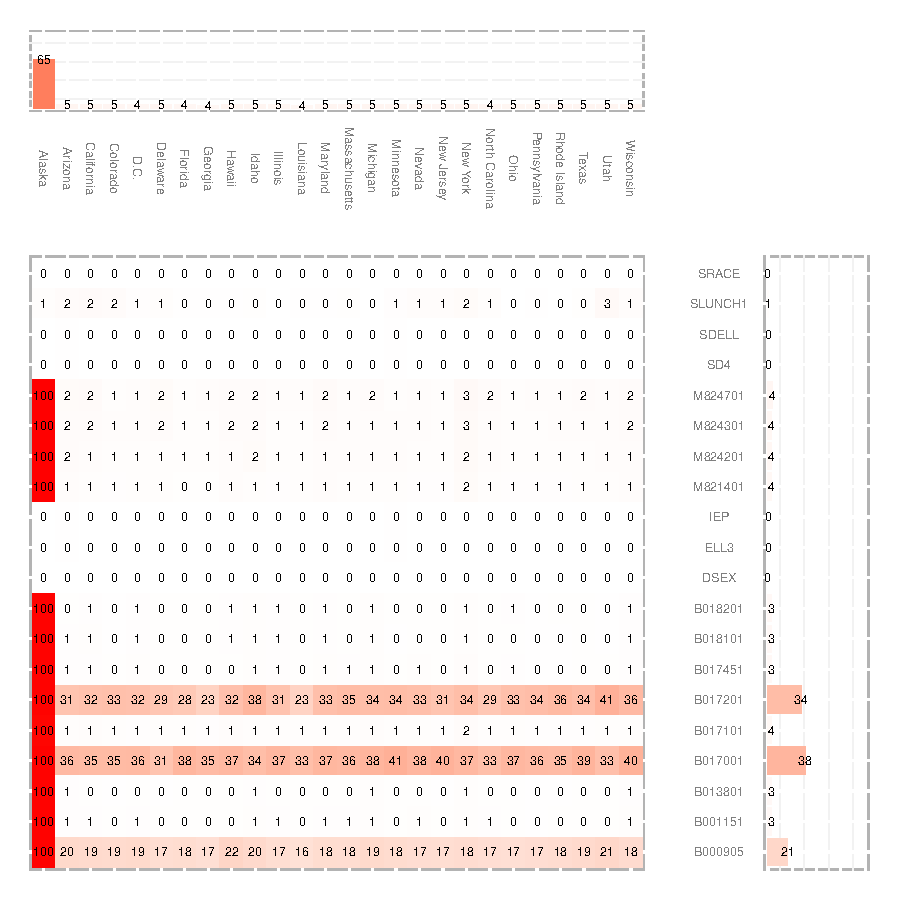
\includegraphics[width=\textwidth]{../Figures2009/g4math-missing.pdf}
\caption{Covariate missingness for grade 4 math}
\label{fig:g4math:missing}
\end{center}
\end{figure}

\begin{figure}[h]
\begin{center}
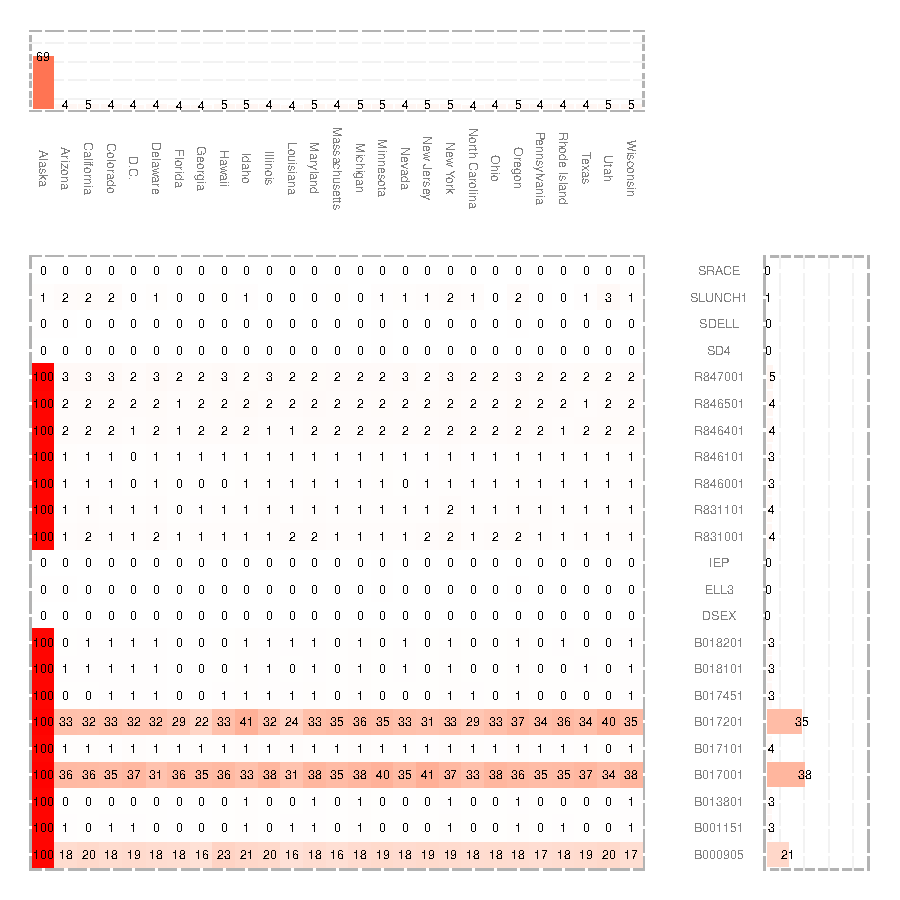
\includegraphics[width=\textwidth]{../Figures2009/g4read-missing.pdf}
\caption{Covariate missingness for grade 4 reading}
\label{fig:g4reading:missing}
\end{center}
\end{figure}

\begin{figure}[h]
\begin{center}
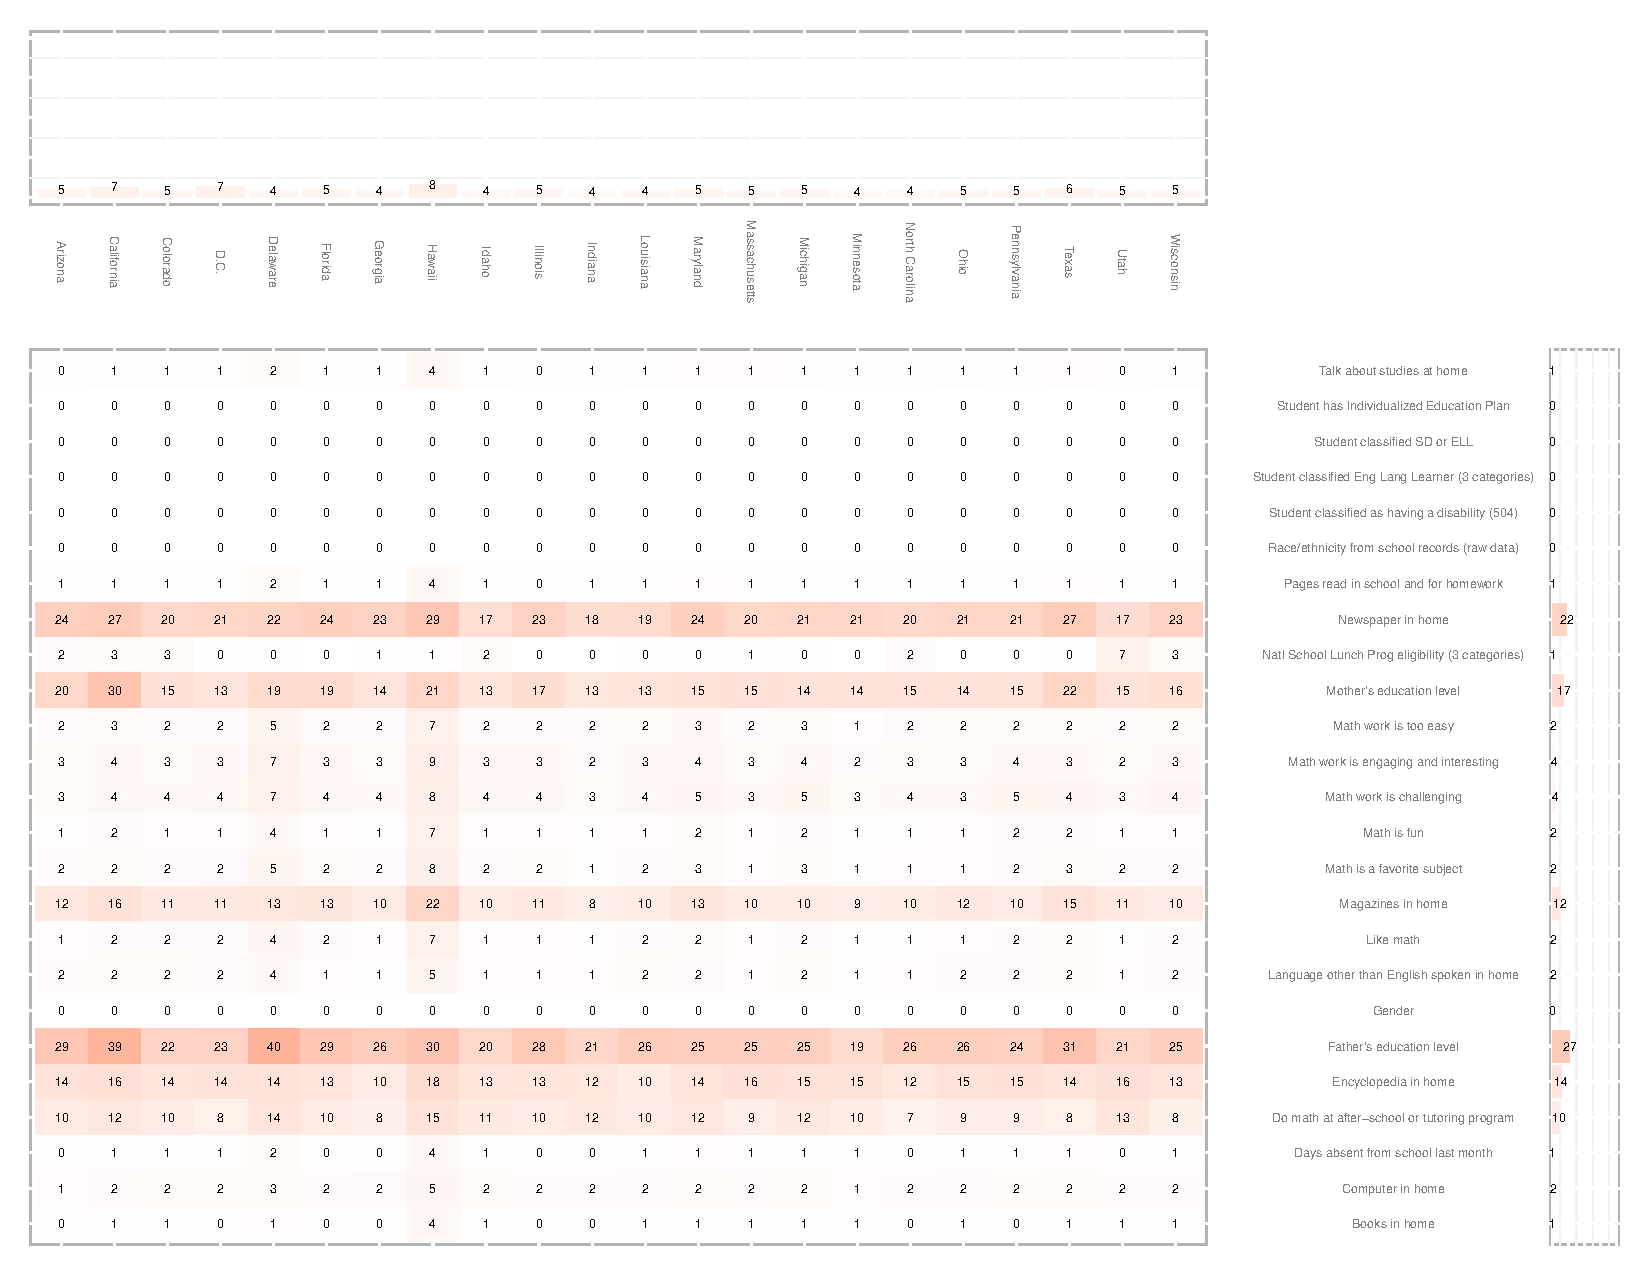
\includegraphics[width=\textwidth]{../Figures2009/g8math-missing.pdf}
\caption{Covariate missingness for grade 8 math}
\label{fig:g8math:missing}
\end{center}
\end{figure}

\begin{figure}[h]
\begin{center}
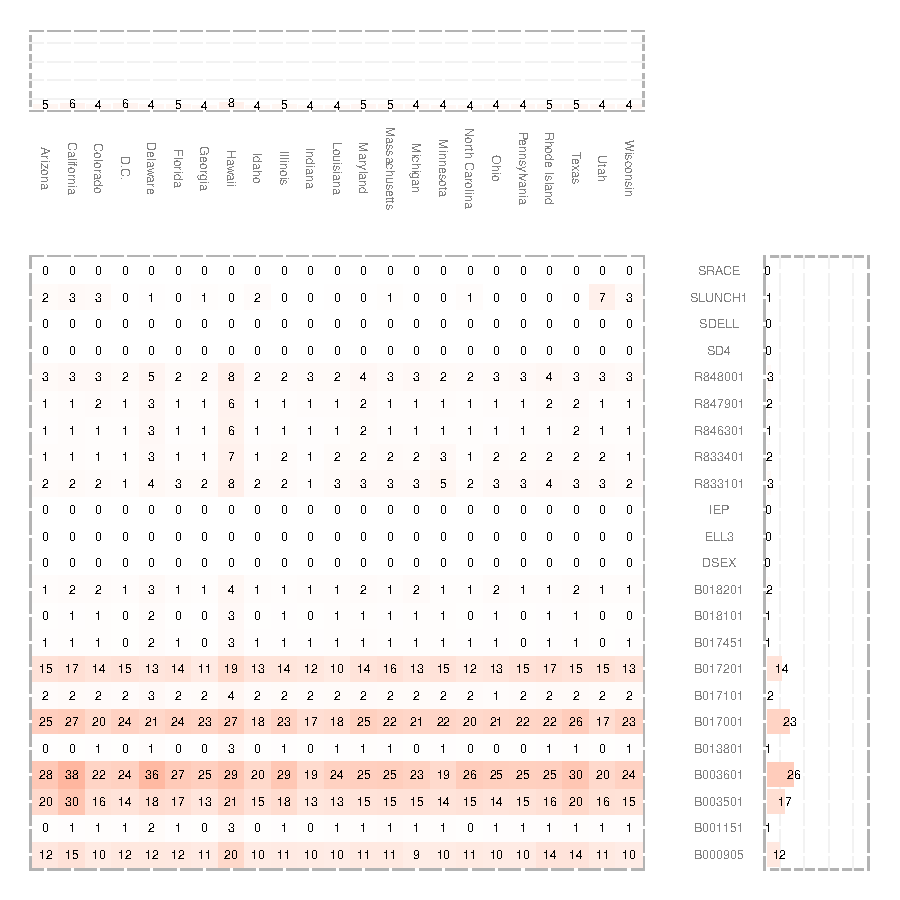
\includegraphics[width=\textwidth]{../Figures2009/g8read-missing.pdf}
\caption{Covariate missingness for grade 8 reading}
\label{fig:g8reading:missing}
\end{center}
\end{figure}


%==================== Appendix D ====================================================================
\clearpage
\addcontentsline{toc}{subsection}{Appendix D: Loess Regression Plots}
\section*{Appendix D\\Loess Regression Plots}
\label{appendixD}

\begin{figure}[h!]
\begin{center}
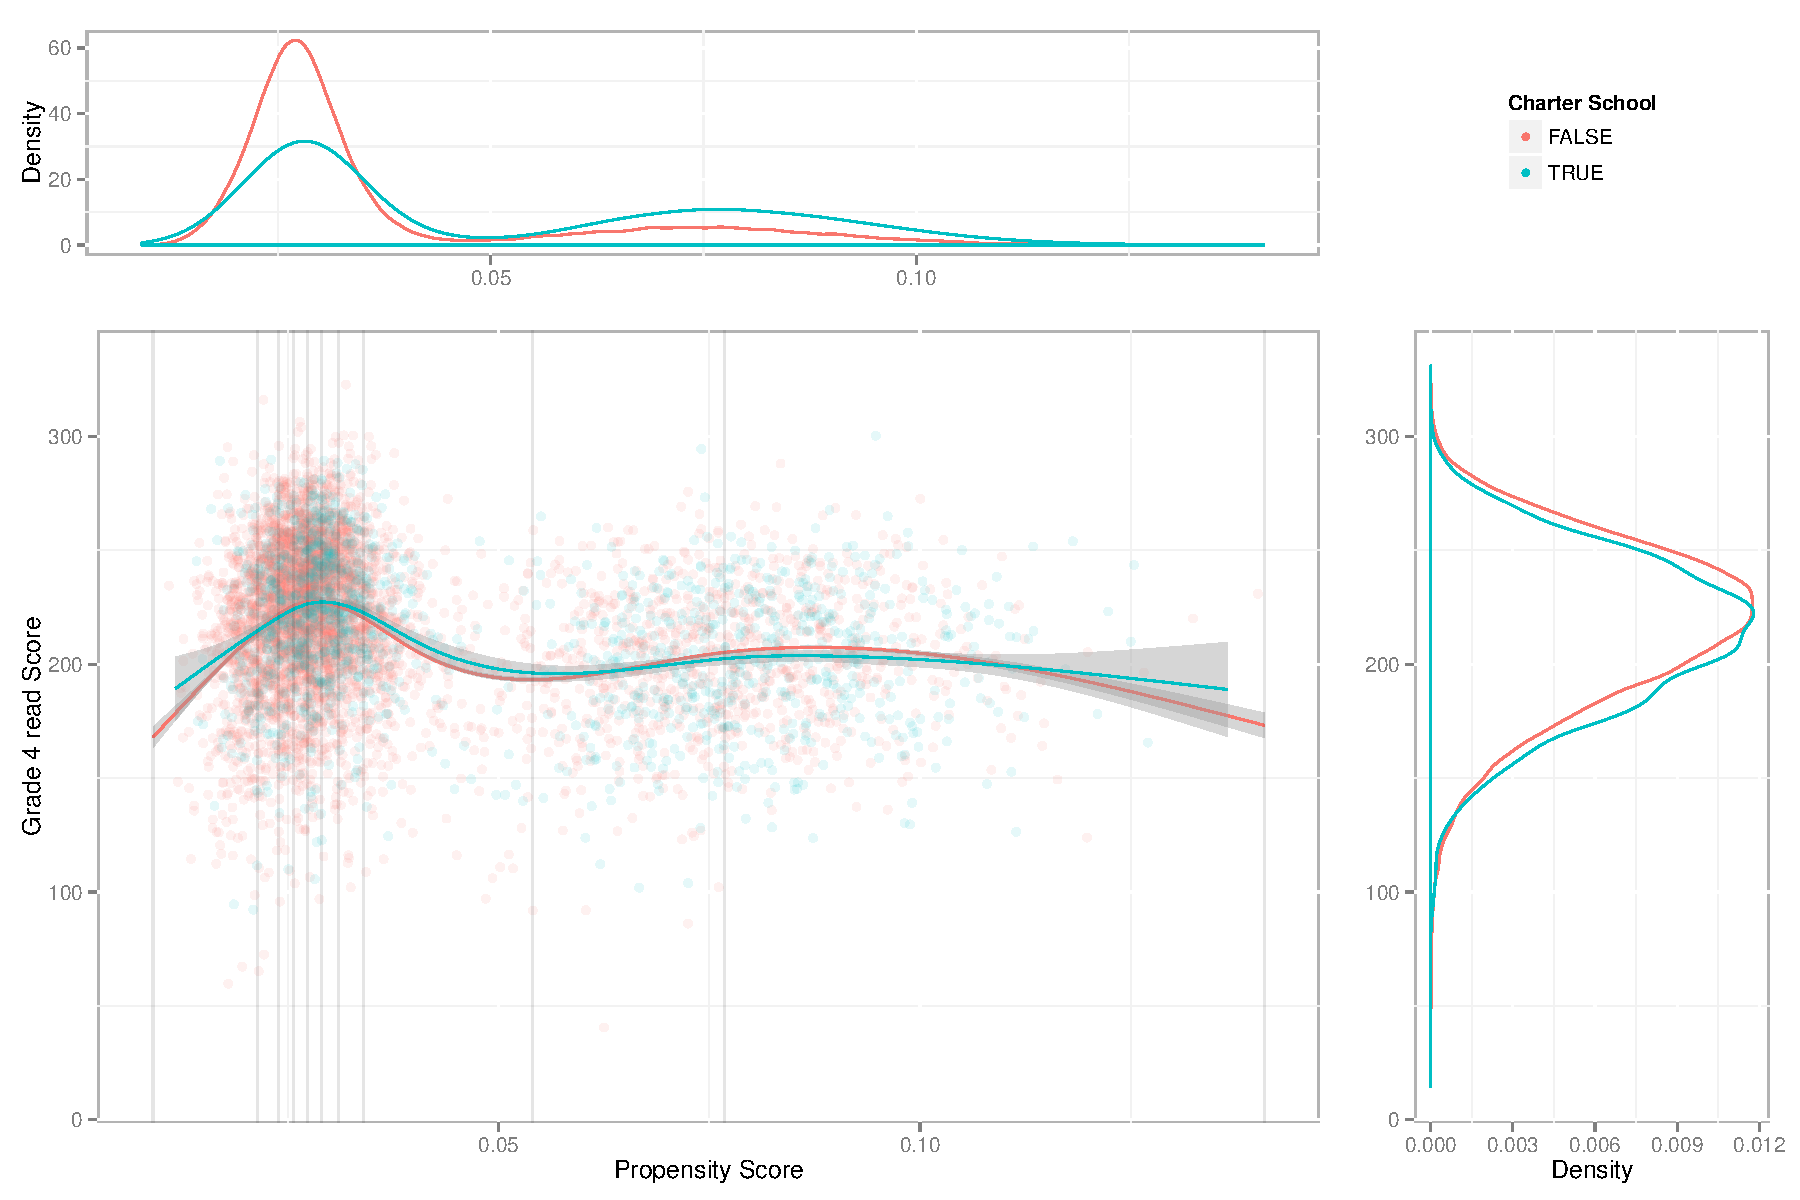
\includegraphics[height=.4\textheight]{../Figures2009/g4read-loess.pdf}
\caption{Loess regression assessment plot: Grade 4 reading}
\label{fig:g4read:loess}
\end{center}
\end{figure}

\begin{figure}[h!]
\begin{center}
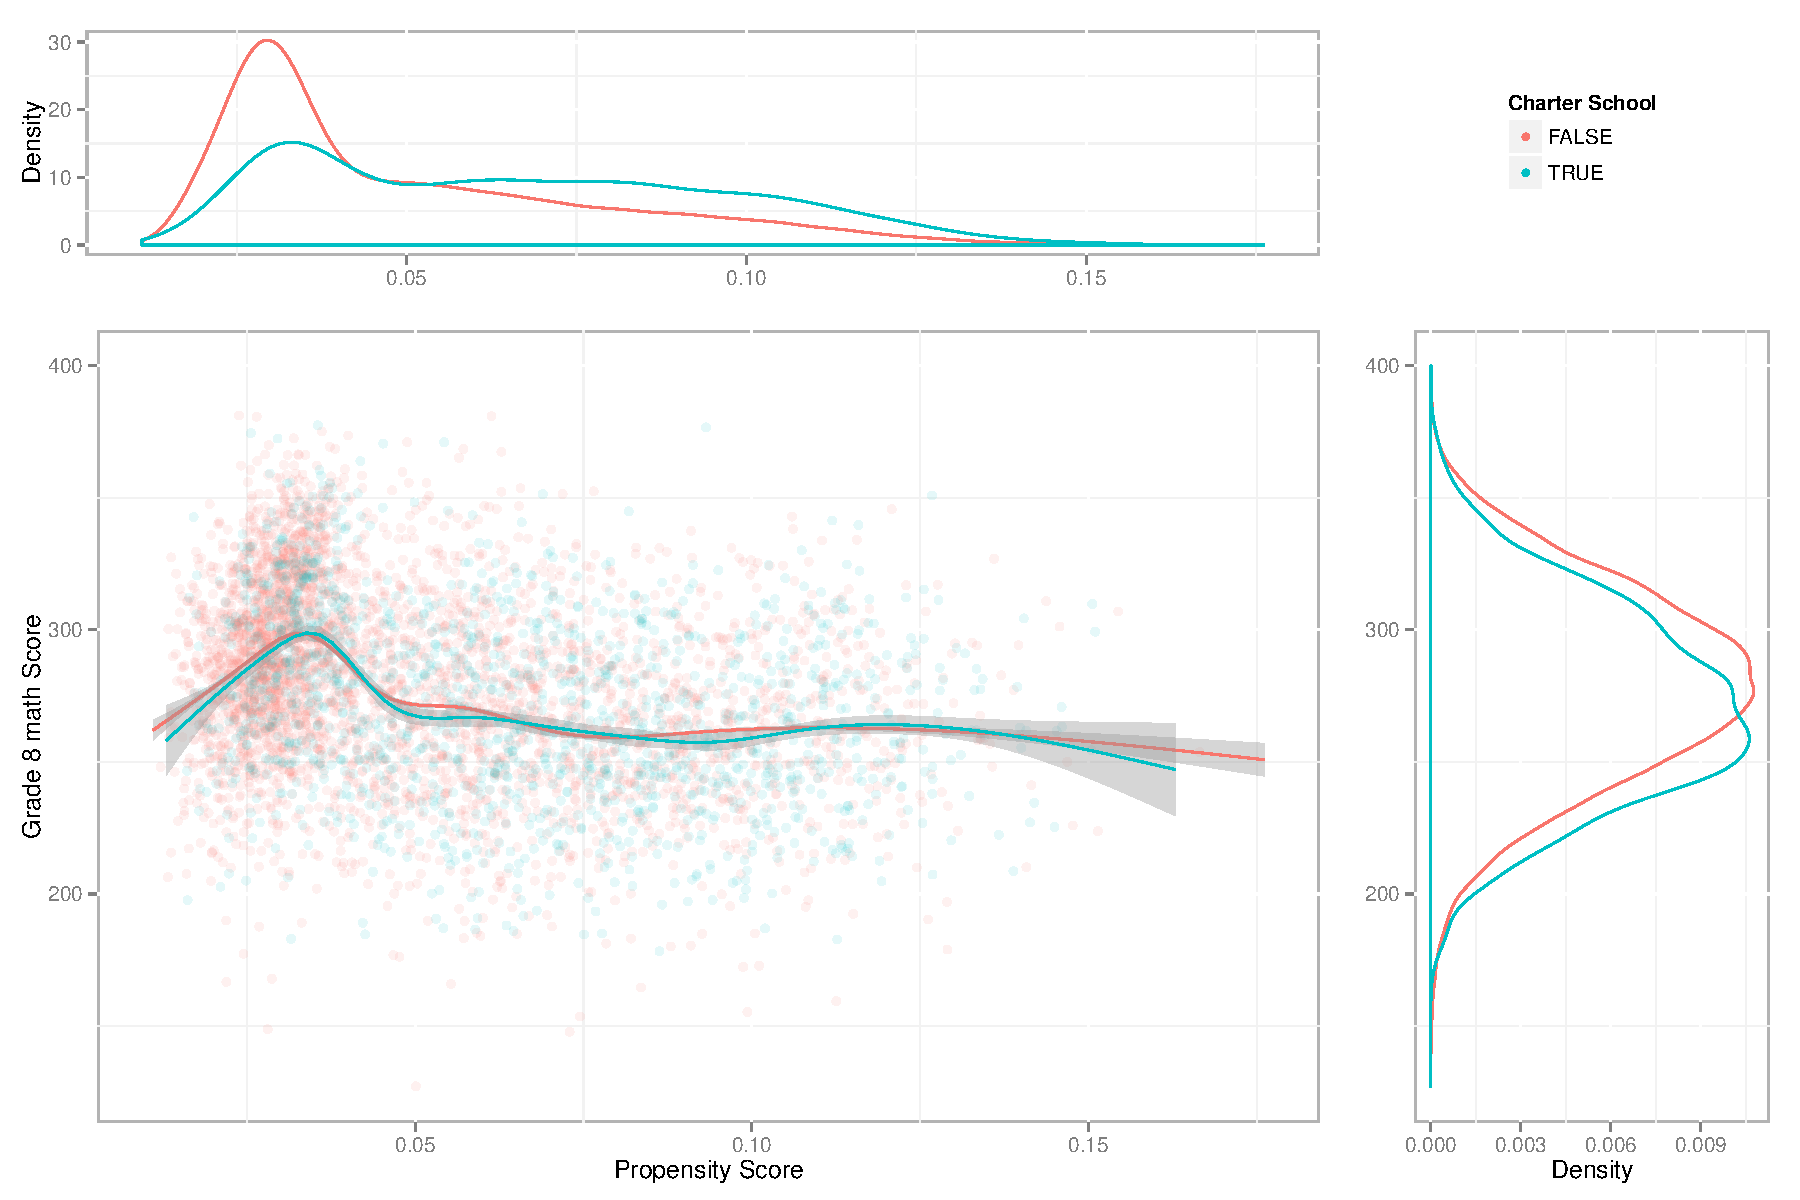
\includegraphics[height=.4\textheight]{../Figures2009/g8math-loess.pdf}
\caption{Loess regression assessment plot: Grade 8 math}
\label{fig:g8math:loess}
\end{center}
\end{figure}

\begin{figure}[h!]
\begin{center}
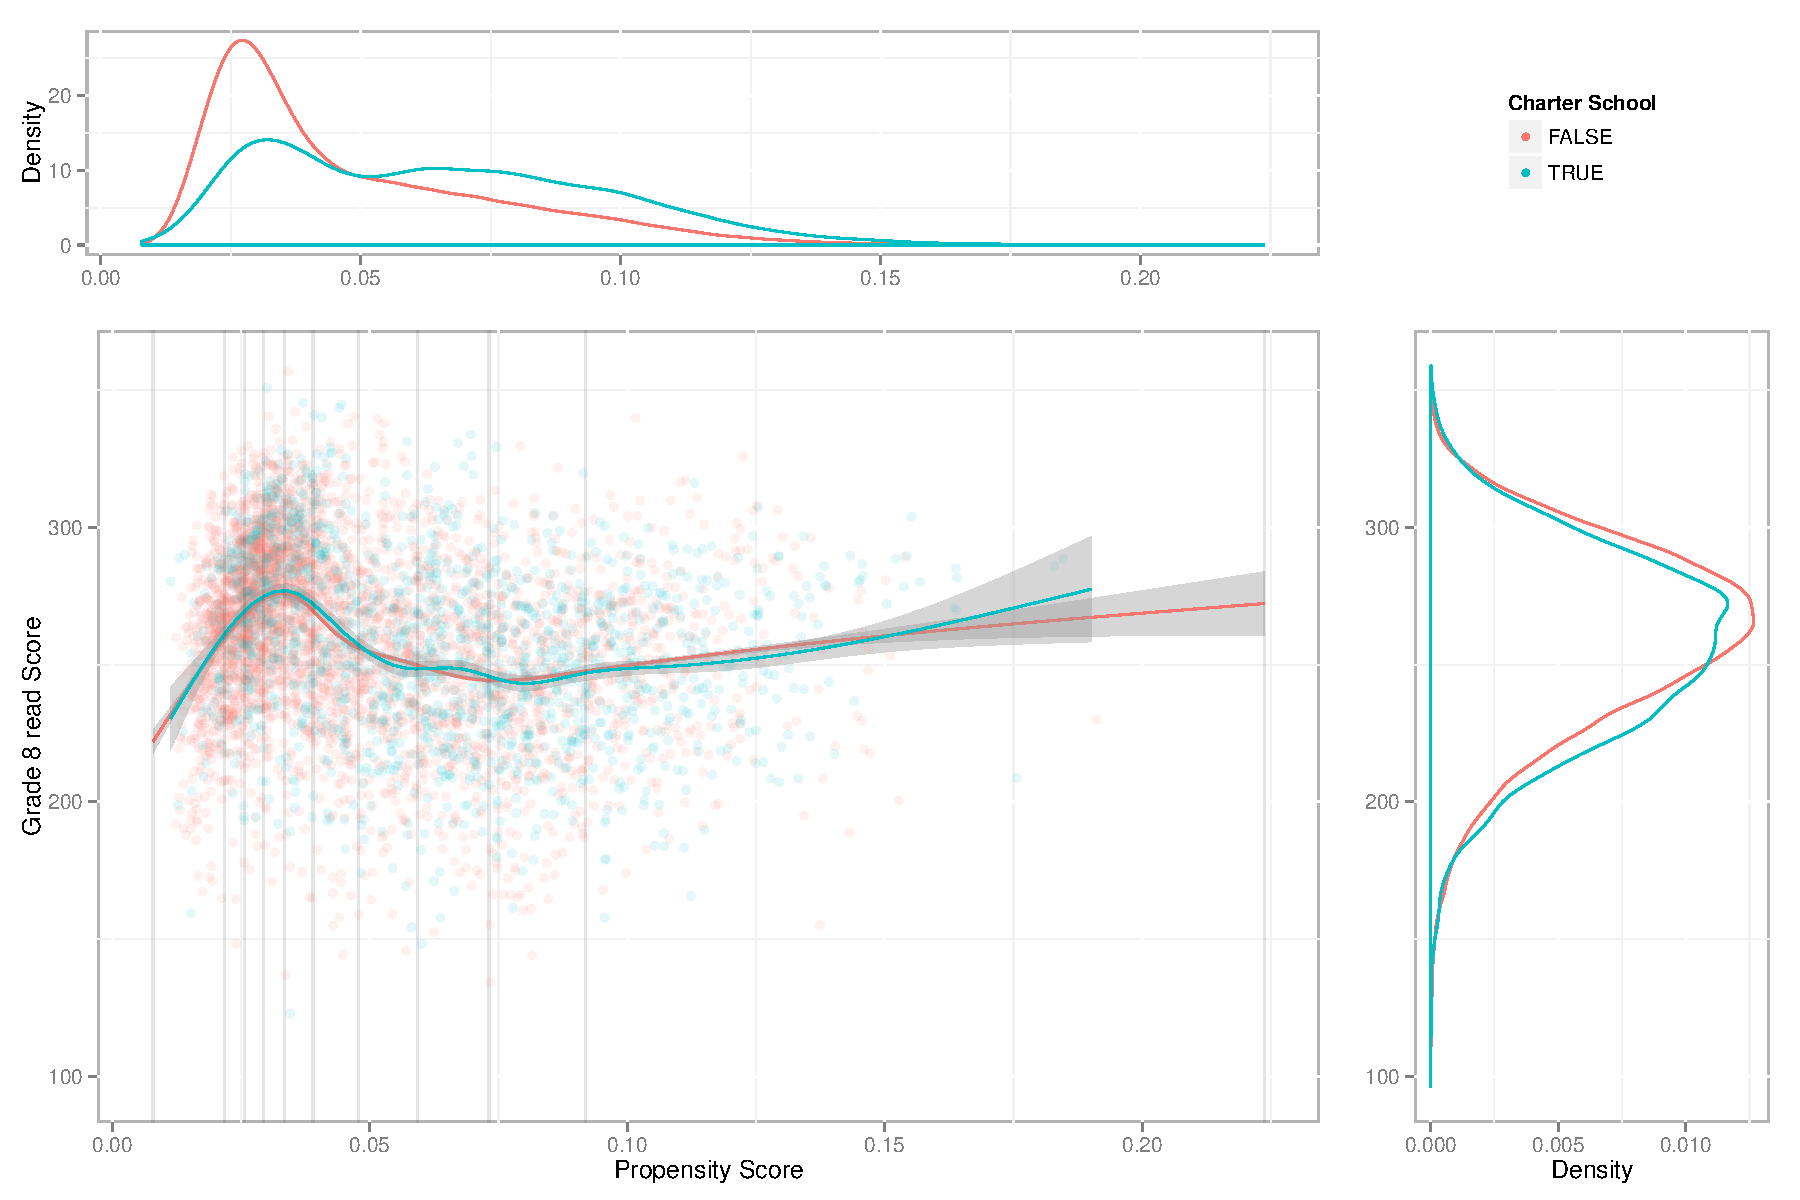
\includegraphics[height=.4\textheight]{../Figures2009/g8read-loess.pdf}
\caption{Loess regression assessment plot: Grade 8 reading}
\label{fig:g8read:loess}
\end{center}
\end{figure}

\begin{figure}[h!]
\begin{center}
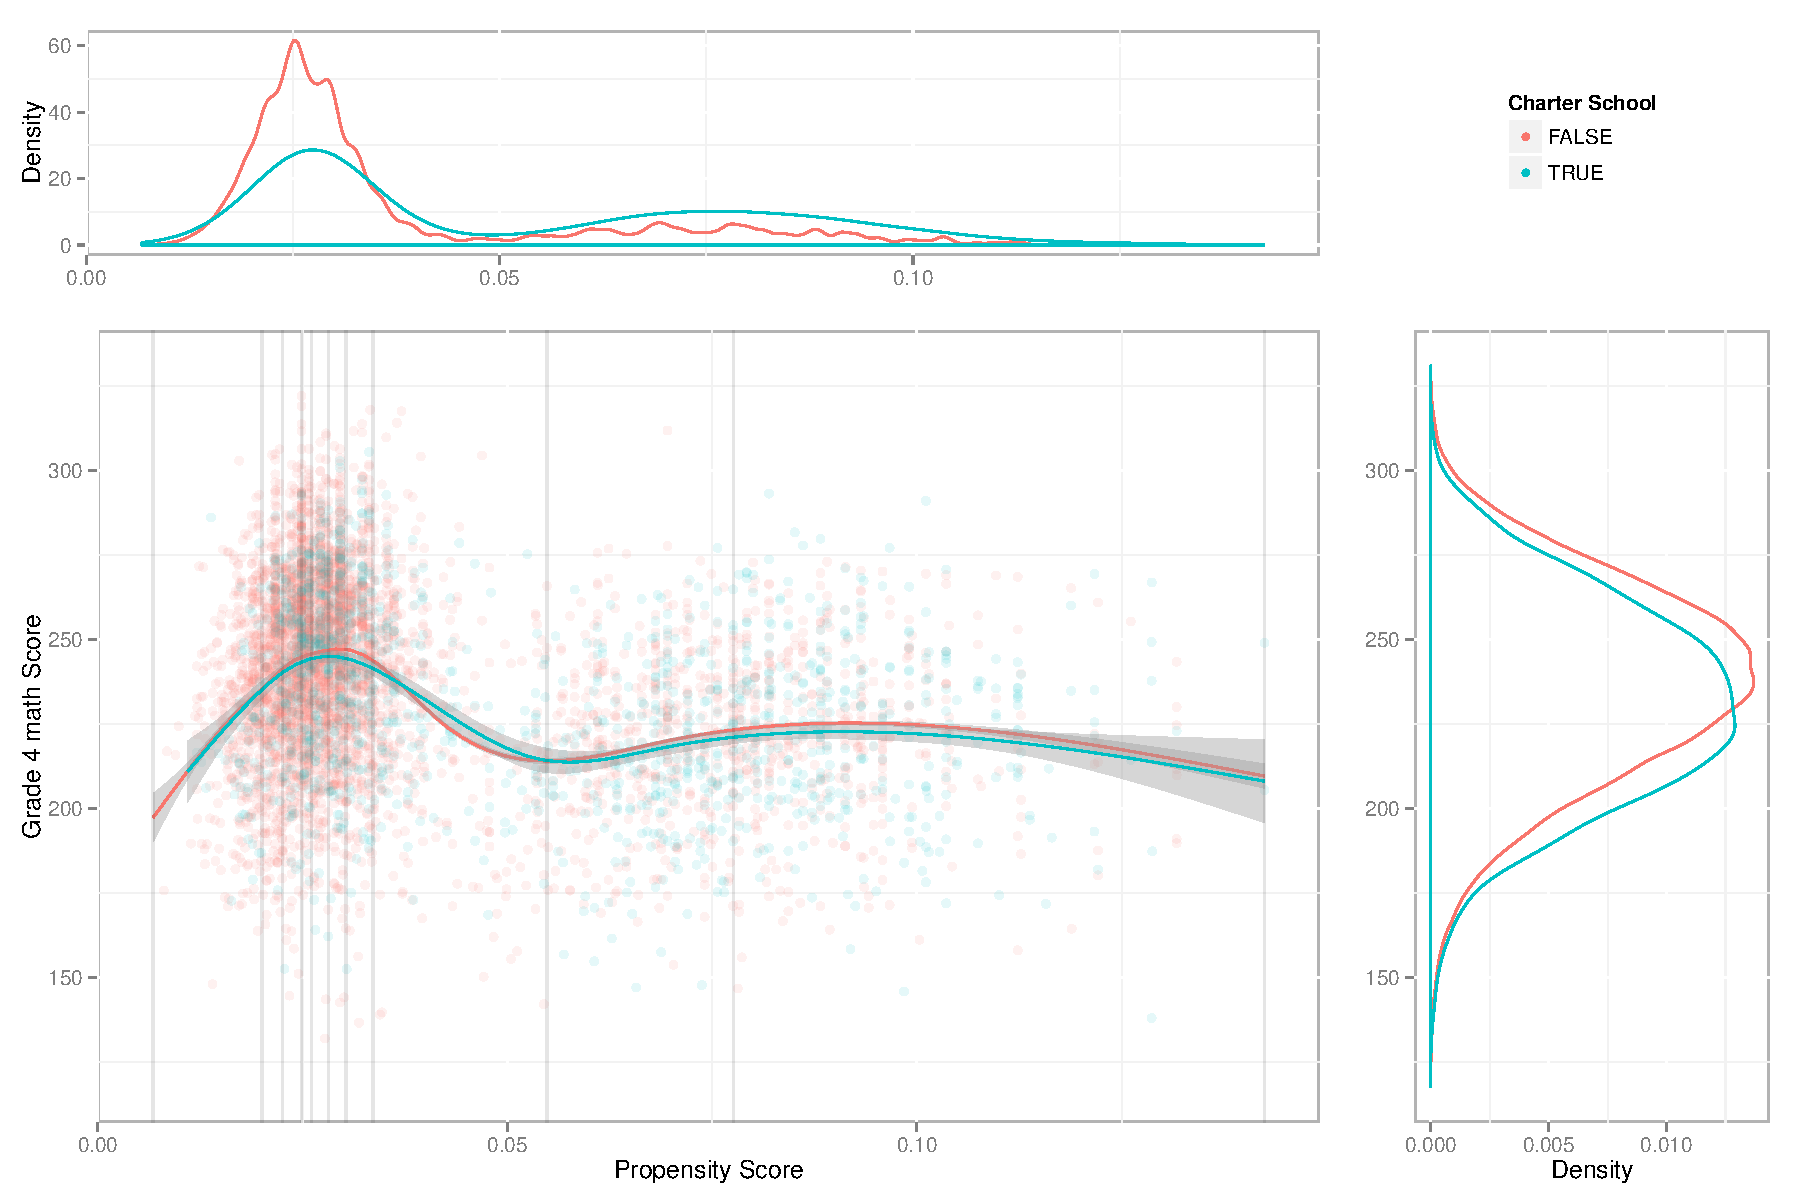
\includegraphics[height=.4\textheight]{../Figures2009/g4math-loessAIC.pdf}
\caption{Loess regression AIC assessment plot: Grade 4 math}
\label{fig:g4math:loessAIC}
\end{center}
\end{figure}

\begin{figure}[h!]
\begin{center}
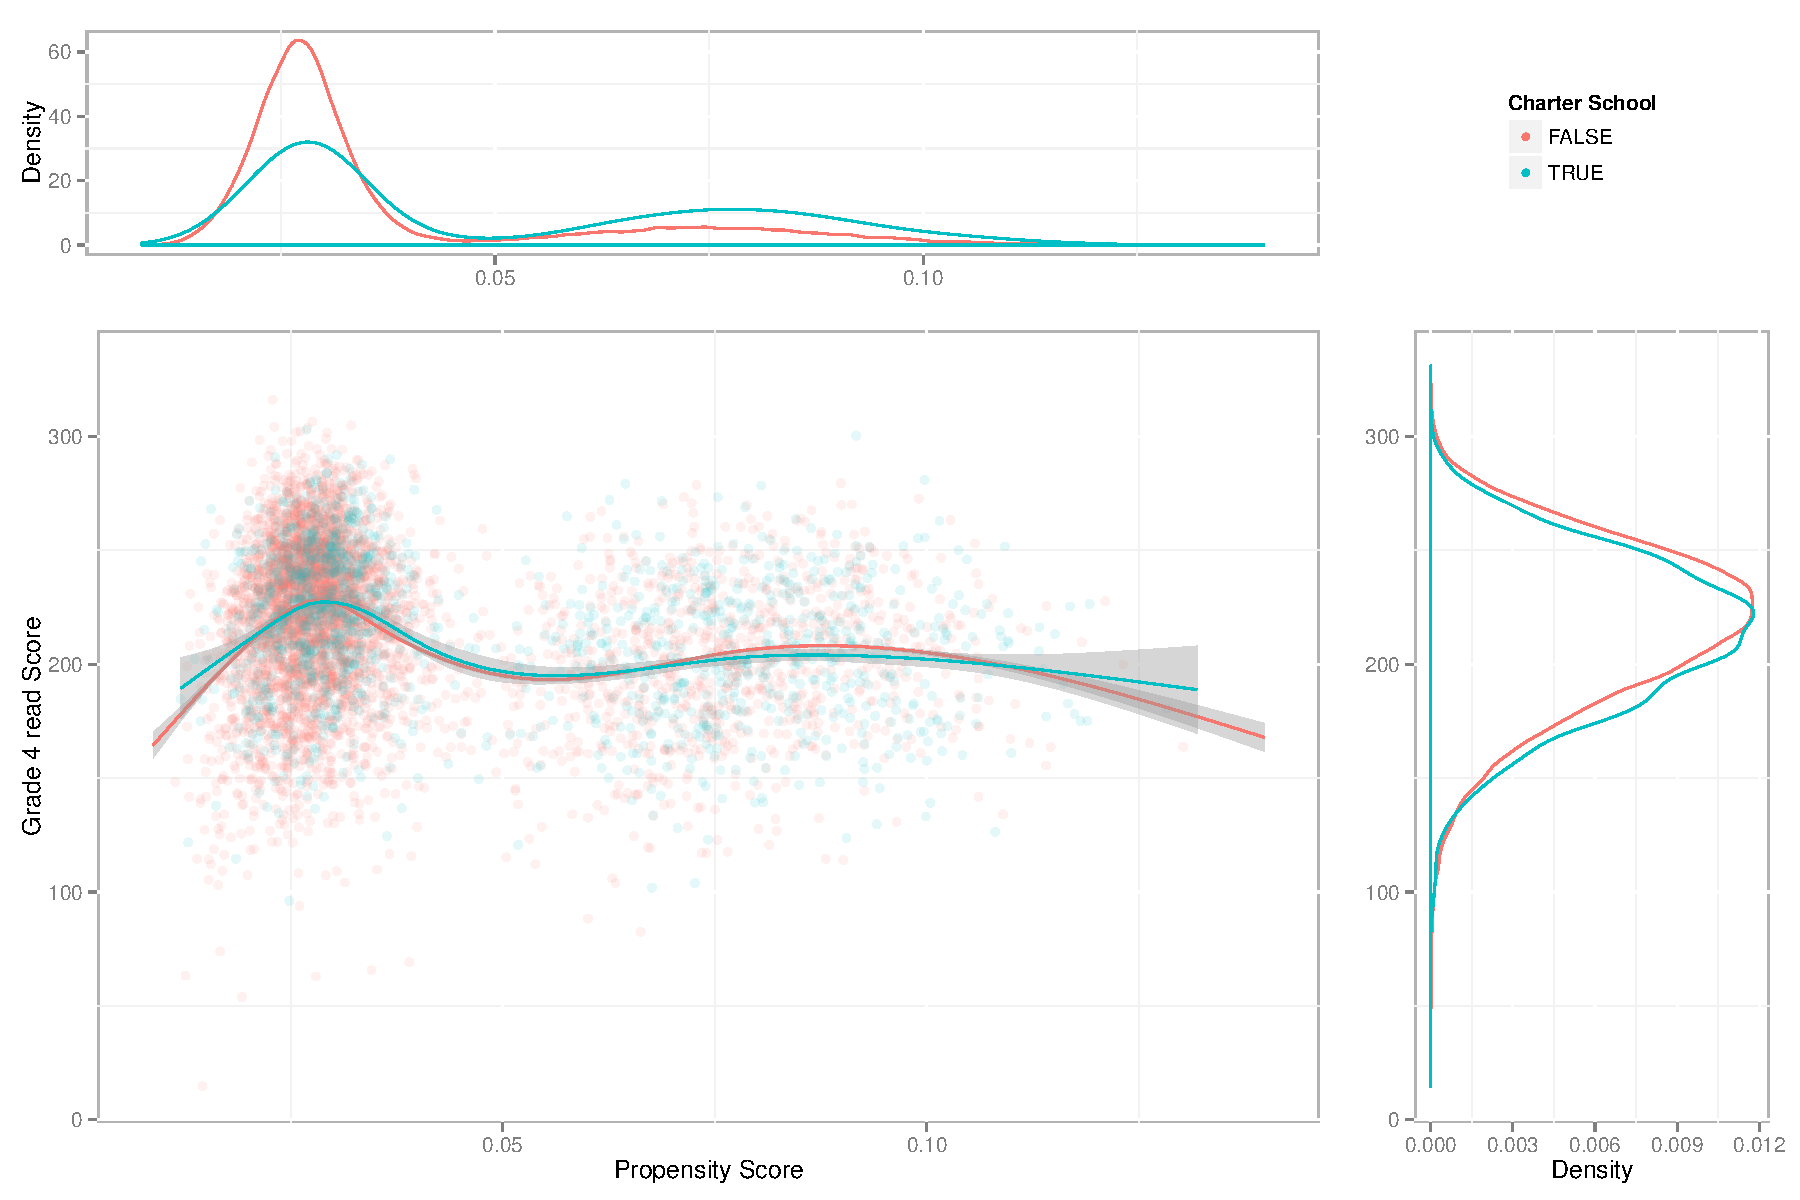
\includegraphics[height=.4\textheight]{../Figures2009/g4read-loessAIC.pdf}
\caption{Loess regression AIC assessment plot: Grade 4 reading}
\label{fig:g4read:loess}
\end{center}
\end{figure}

\begin{figure}[h!]
\begin{center}
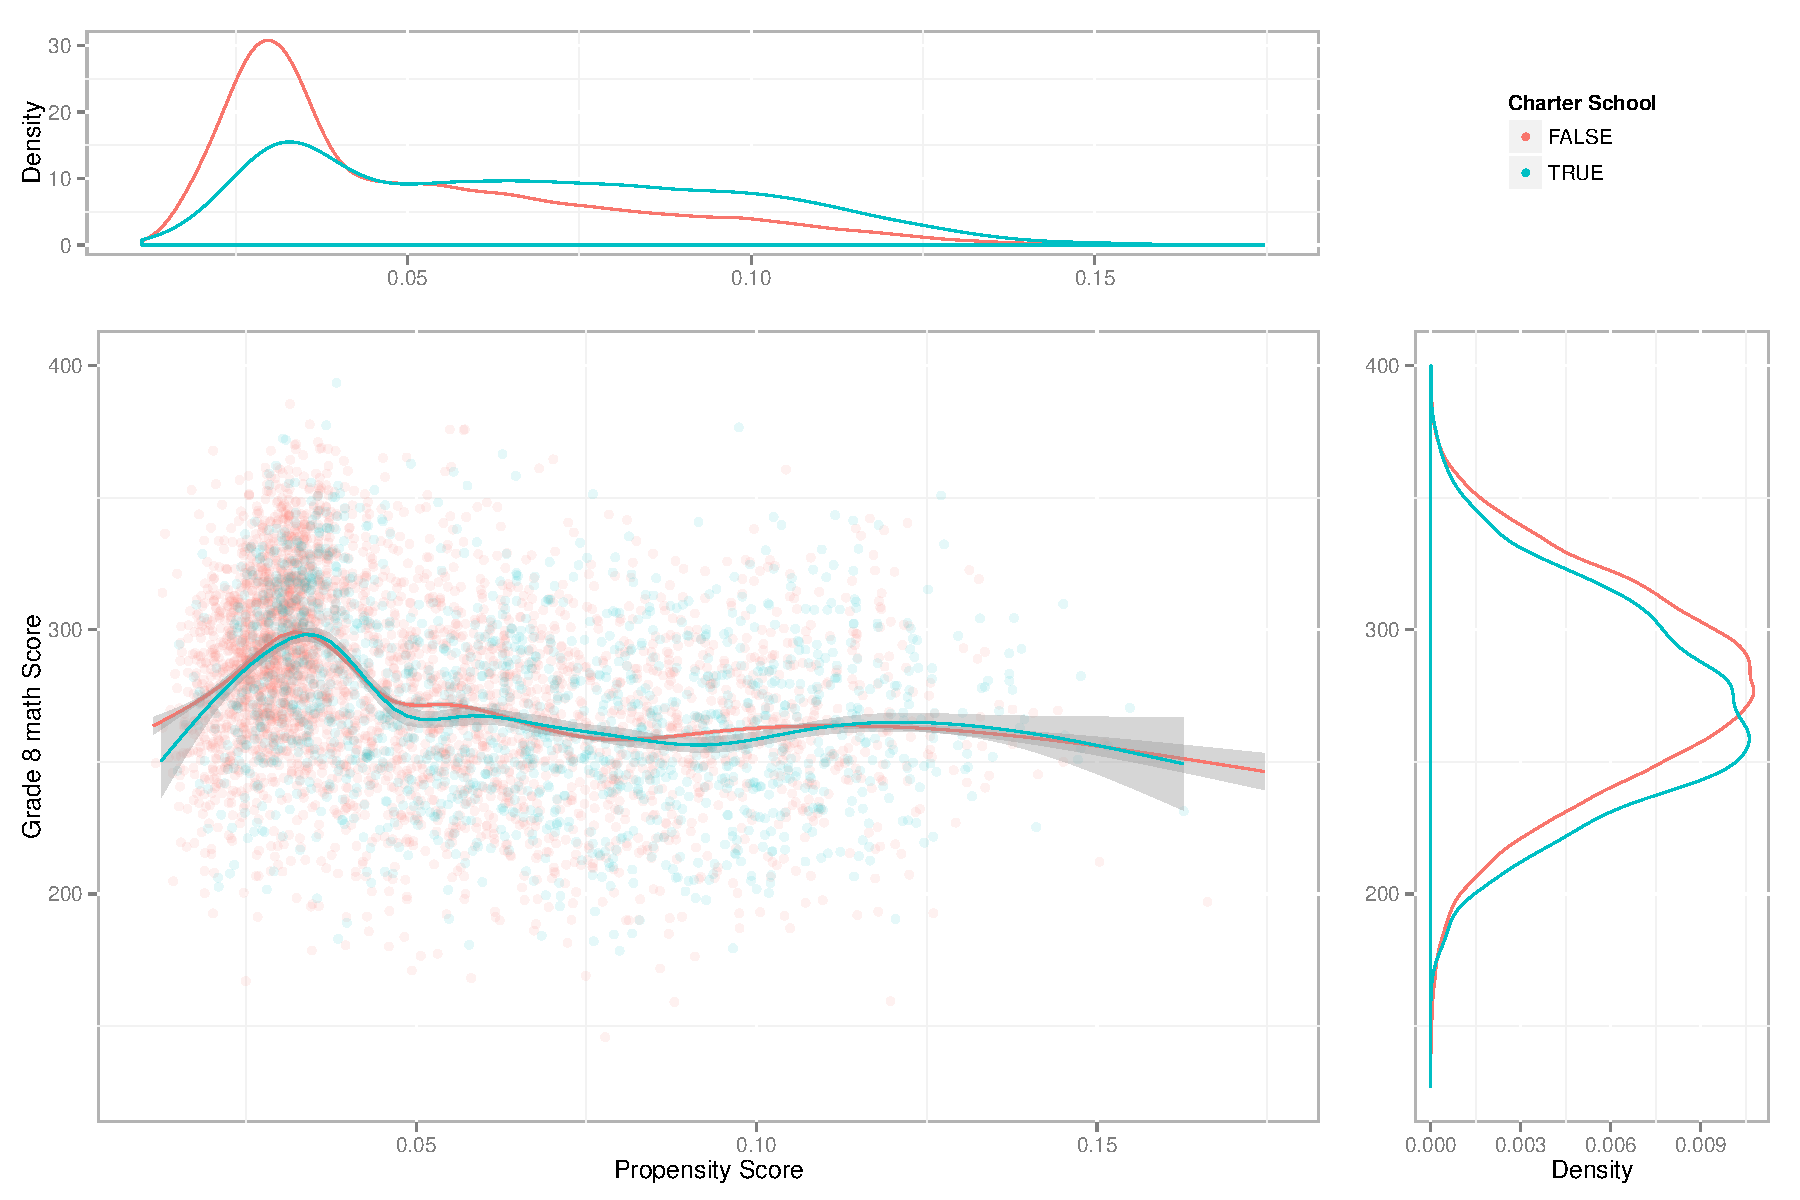
\includegraphics[height=.4\textheight]{../Figures2009/g8math-loessAIC.pdf}
\caption{Loess regression AIC assessment plot: Grade 8 math}
\label{fig:g8math:loess}
\end{center}
\end{figure}

\begin{figure}[h!]
\begin{center}
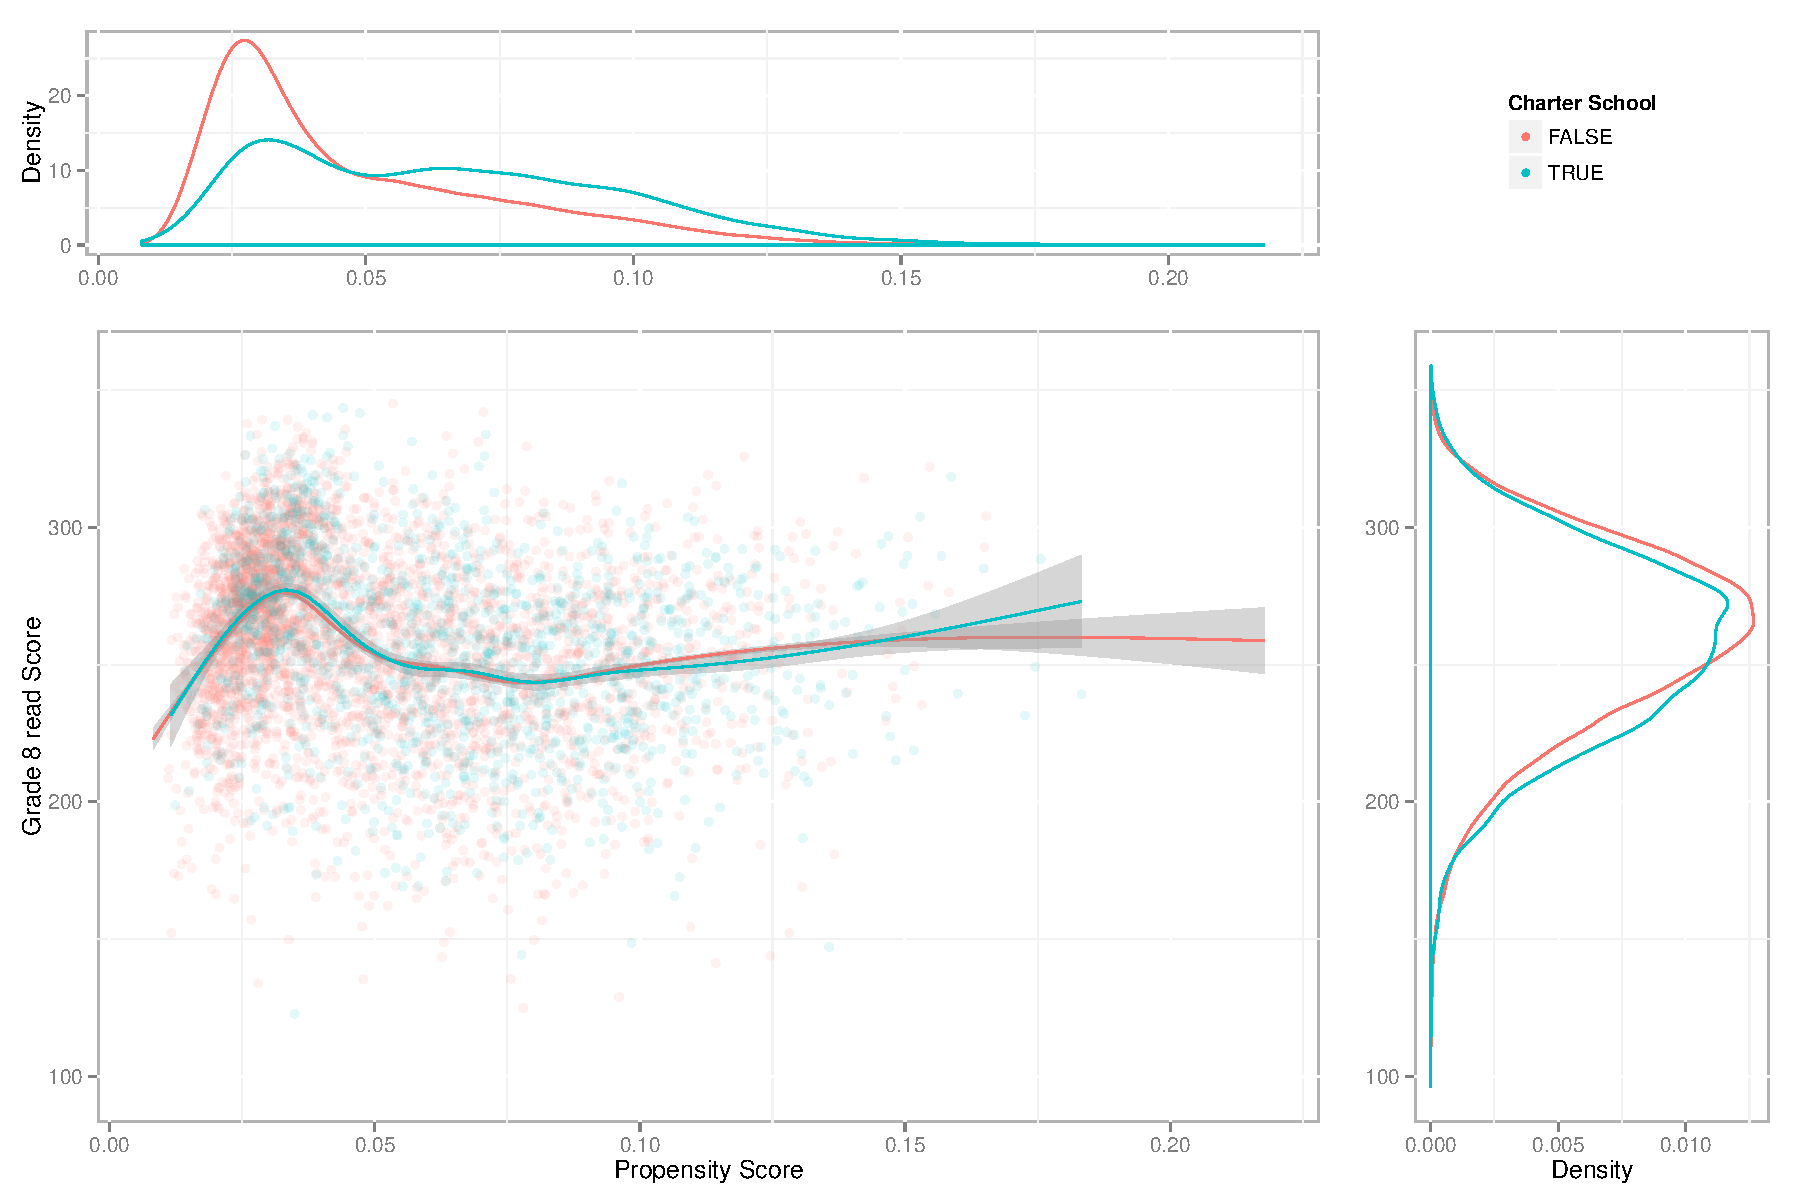
\includegraphics[height=.4\textheight]{../Figures2009/g8read-loessAIC.pdf}
\caption{Loess regression AIC assessment plot: Grade 8 reading}
\label{fig:g8read:loess}
\end{center}
\end{figure}


%==================== Appendix E ====================================================================
\clearpage
\addcontentsline{toc}{subsection}{Appendix E: Covariate Balance Plots}
\section*{Appendix E\\Covariate Balance Plots}
\label{appendixE}

% Grade 4 math

\begin{figure}[h!]
\begin{center}
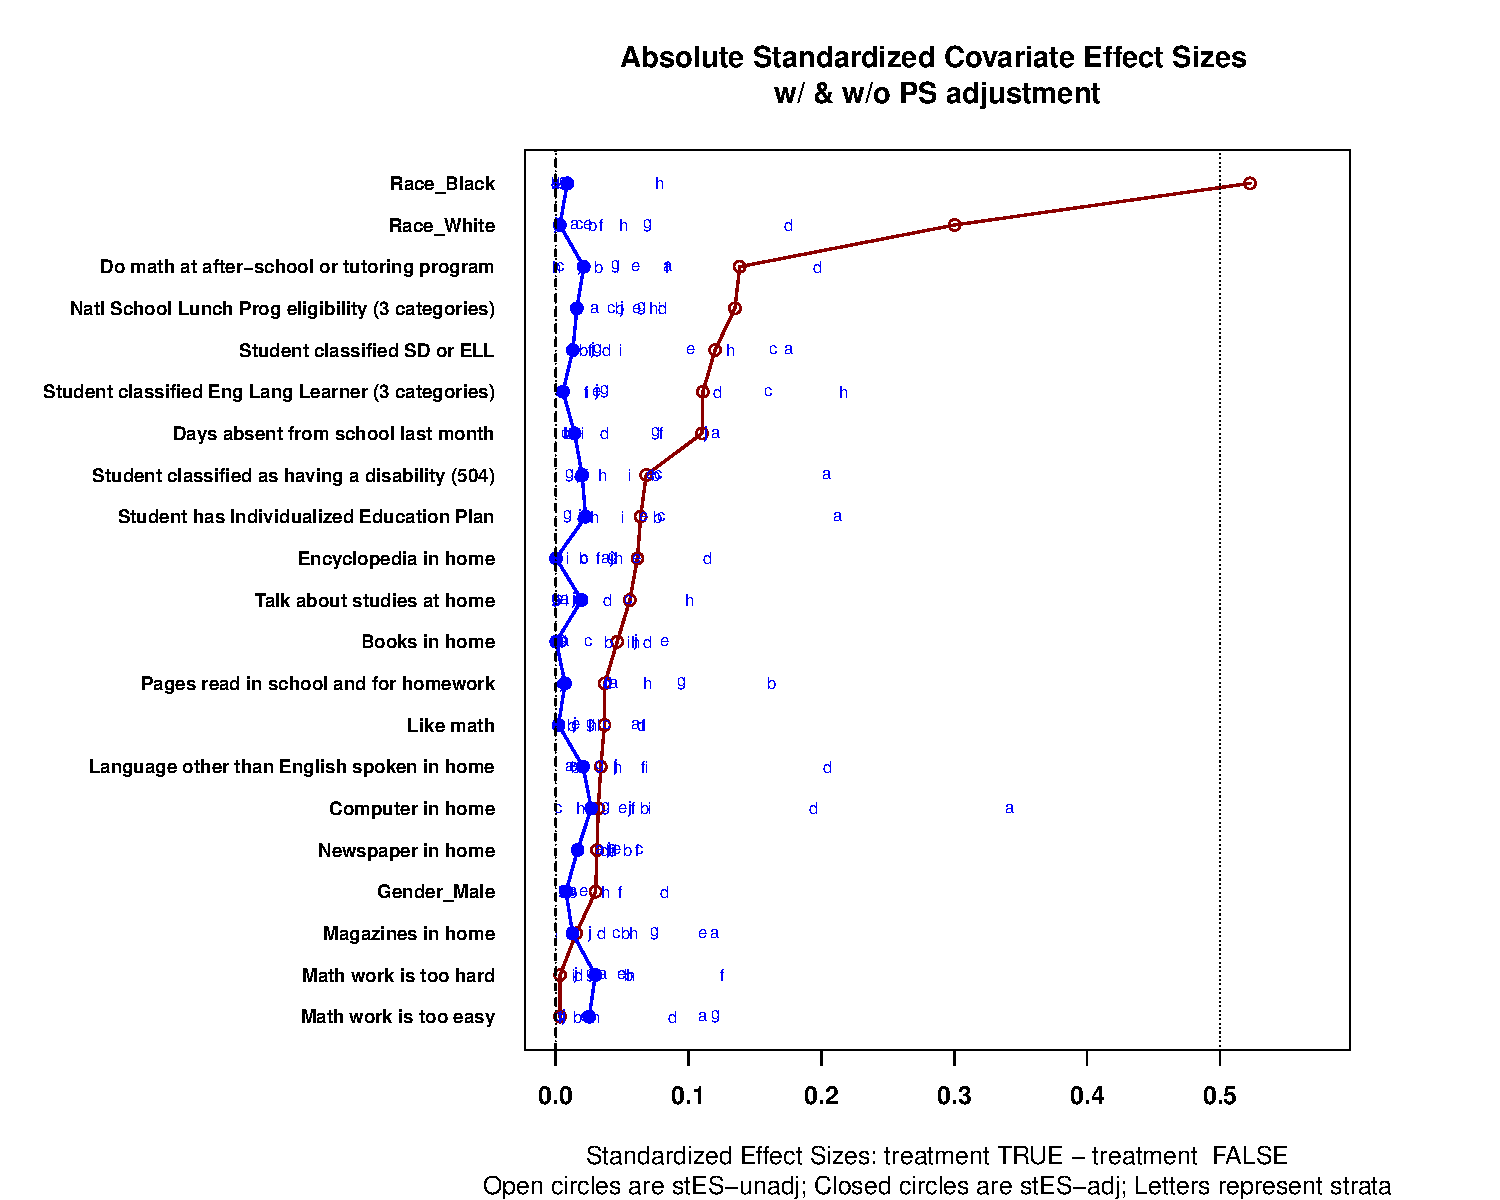
\includegraphics[width=\textwidth]{../Figures2009/g4math-lrAIC-balance.pdf}
\caption{Covariate balance plot for logistic regression AIC stratification: Grade 4 math}
\end{center}
\end{figure}

\begin{figure}
\begin{center}
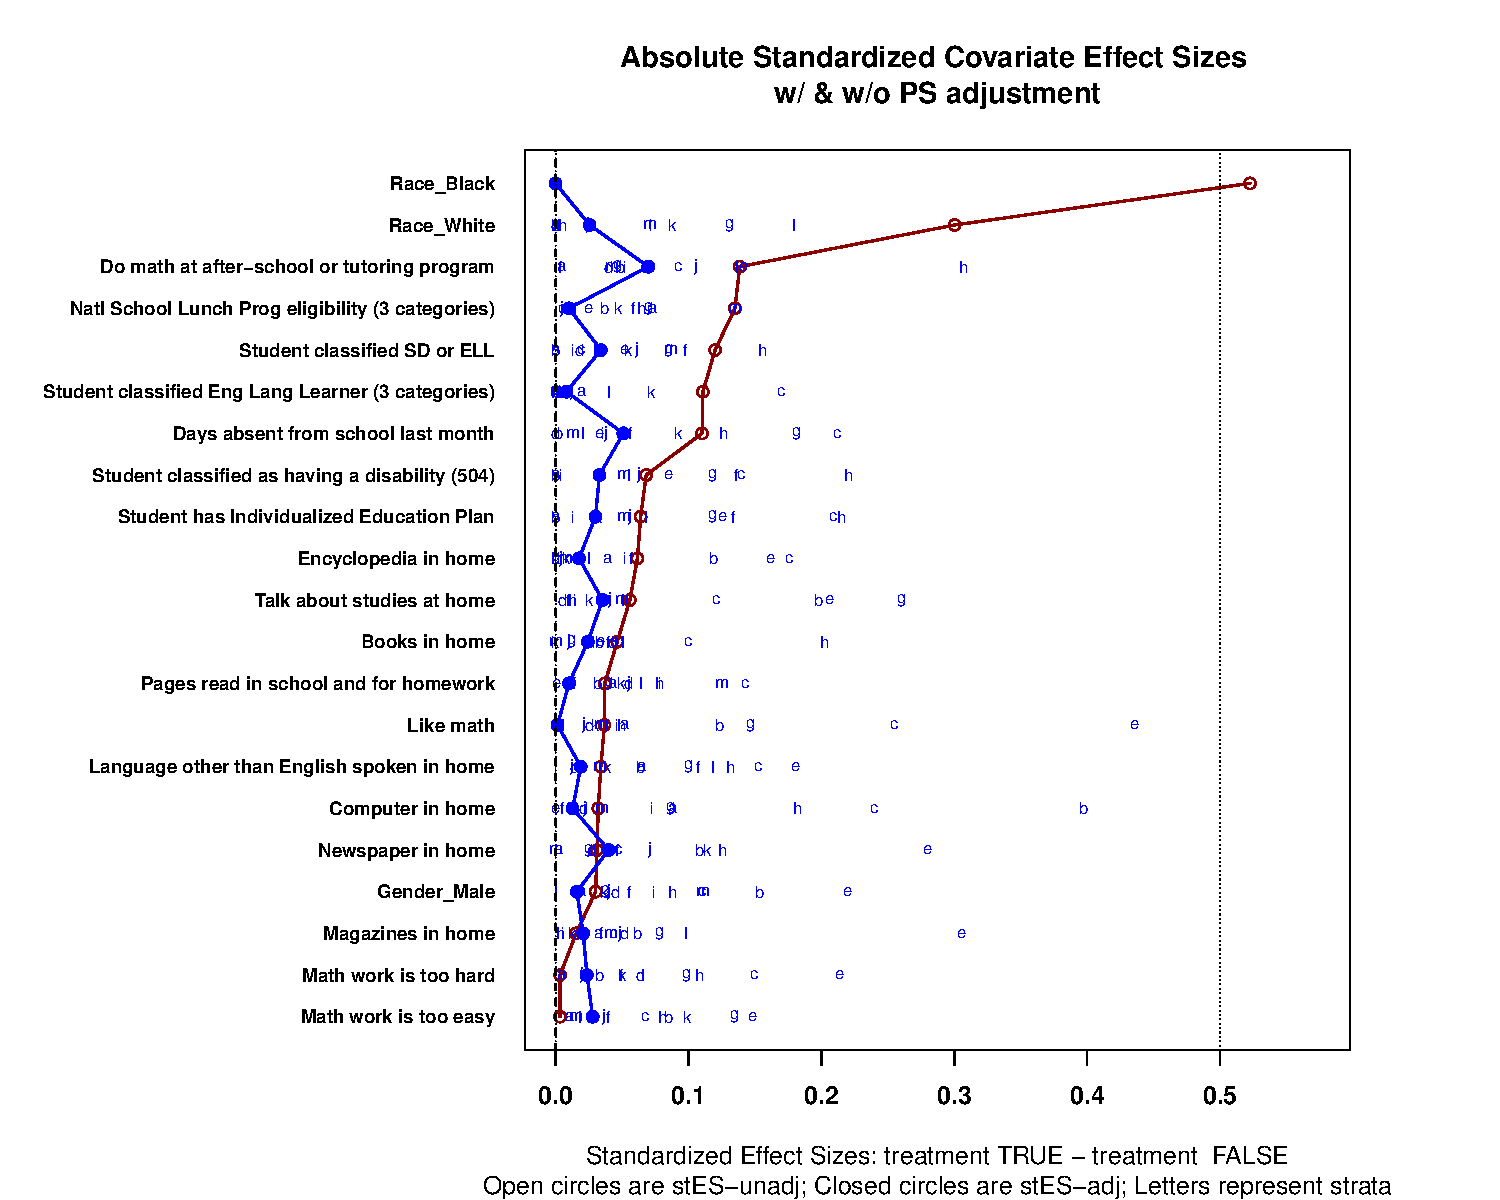
\includegraphics[width=\textwidth]{../Figures2009/g4math-tree-balance.pdf}
\caption{Covariate balance plot for classification tree stratification: Grade 4 math}
\end{center}
\end{figure}

% Grade 4 reading
\begin{figure}
\begin{center}
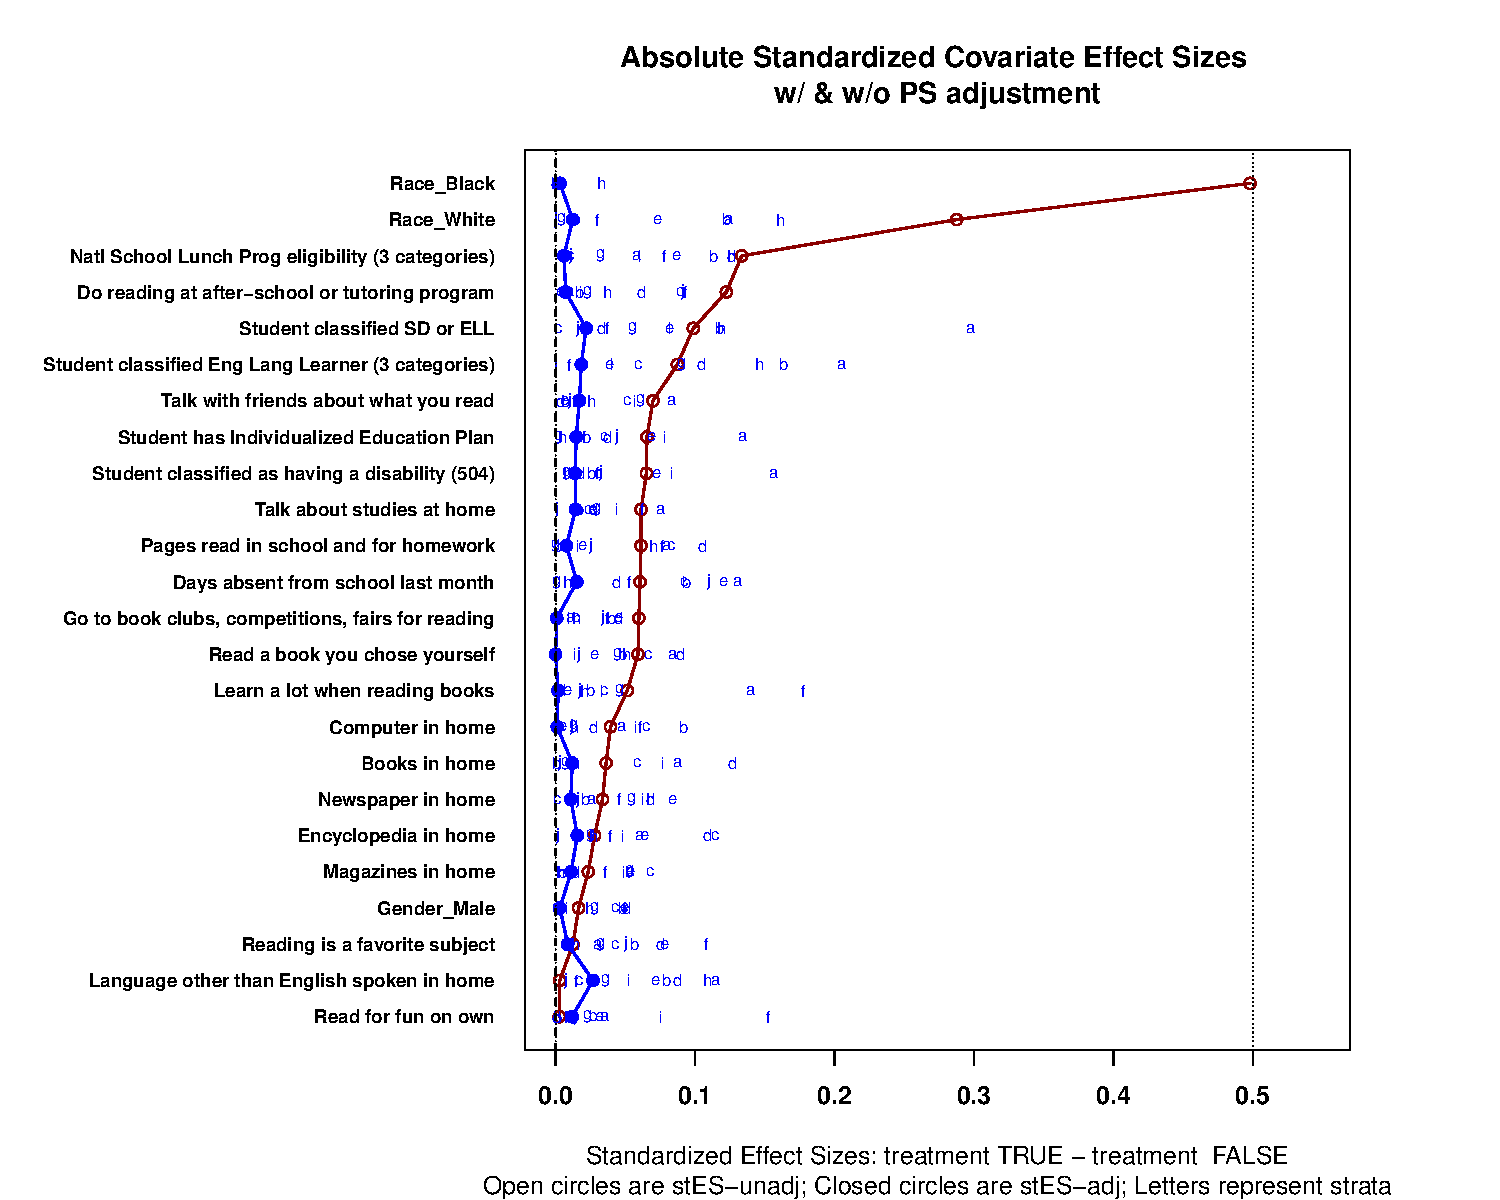
\includegraphics[width=\textwidth]{../Figures2009/g4read-lr-balance.pdf}
\caption{Covariate balance plot for logistic regression stratification: Grade 4 reading}
\end{center}
\end{figure}

\begin{figure}
\begin{center}
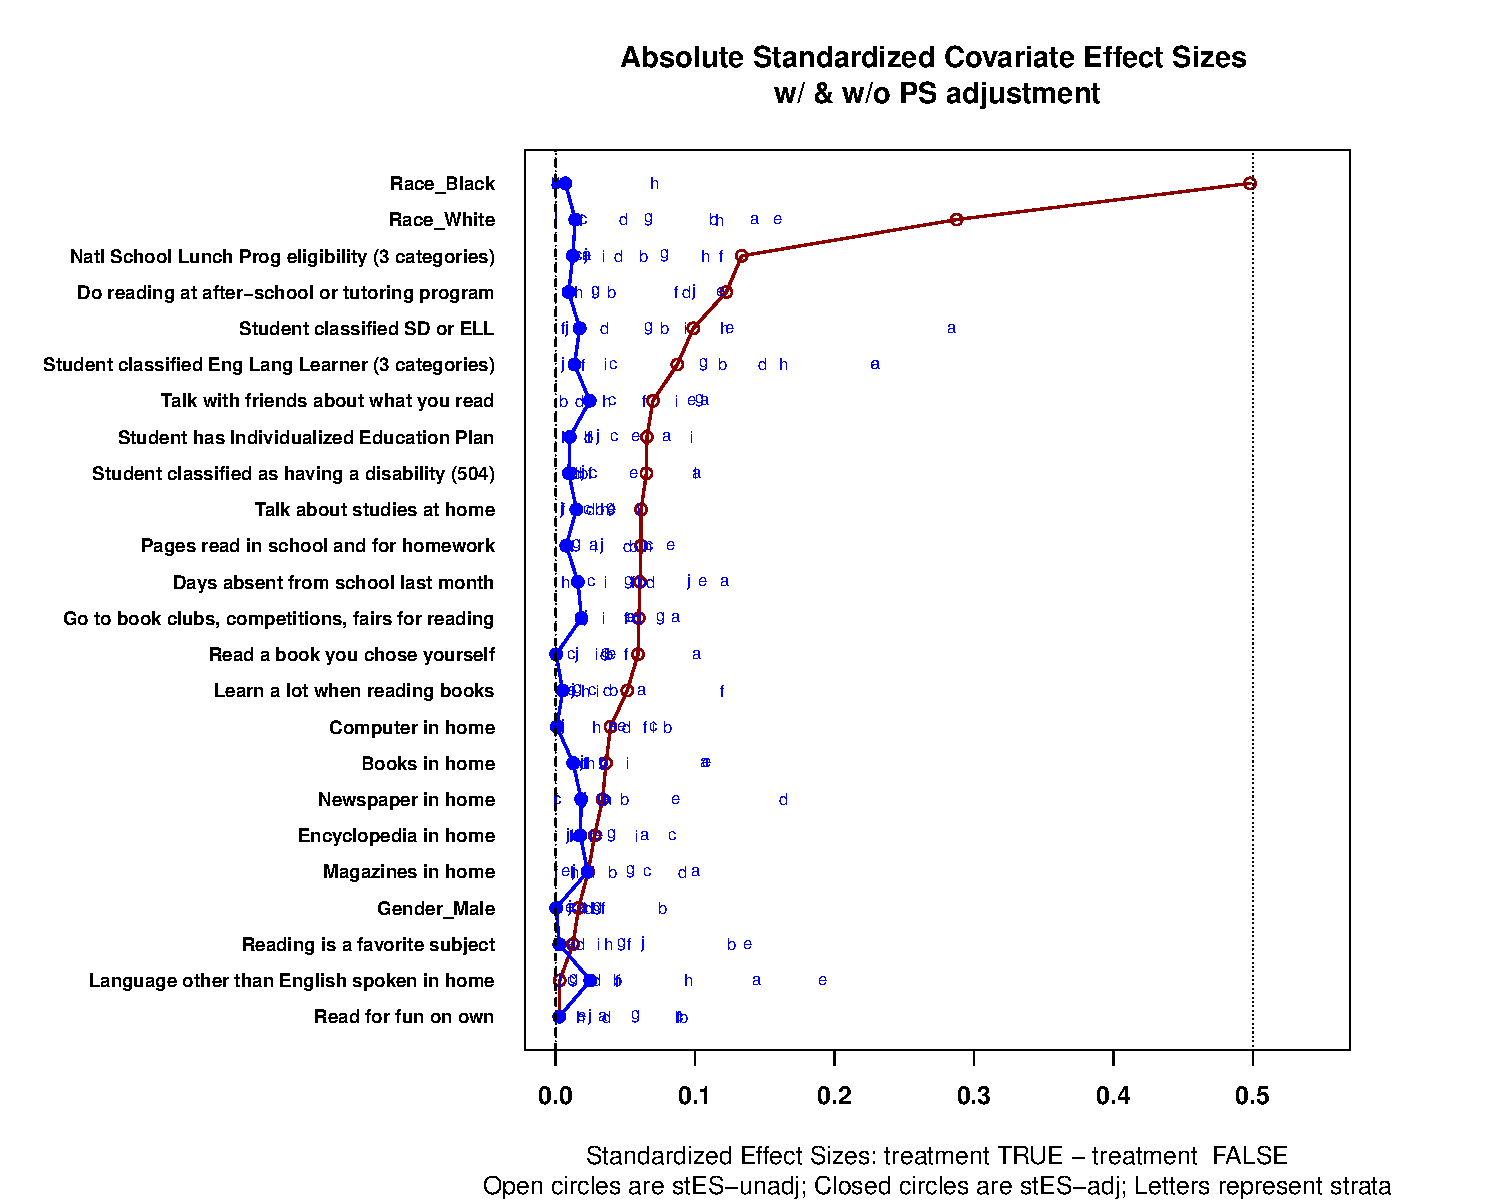
\includegraphics[width=\textwidth]{../Figures2009/g4read-lrAIC-balance.pdf}
\caption{Covariate balance plot for logistic regression AIC stratification: Grade 4 reading}
\end{center}
\end{figure}

\begin{figure}
\begin{center}
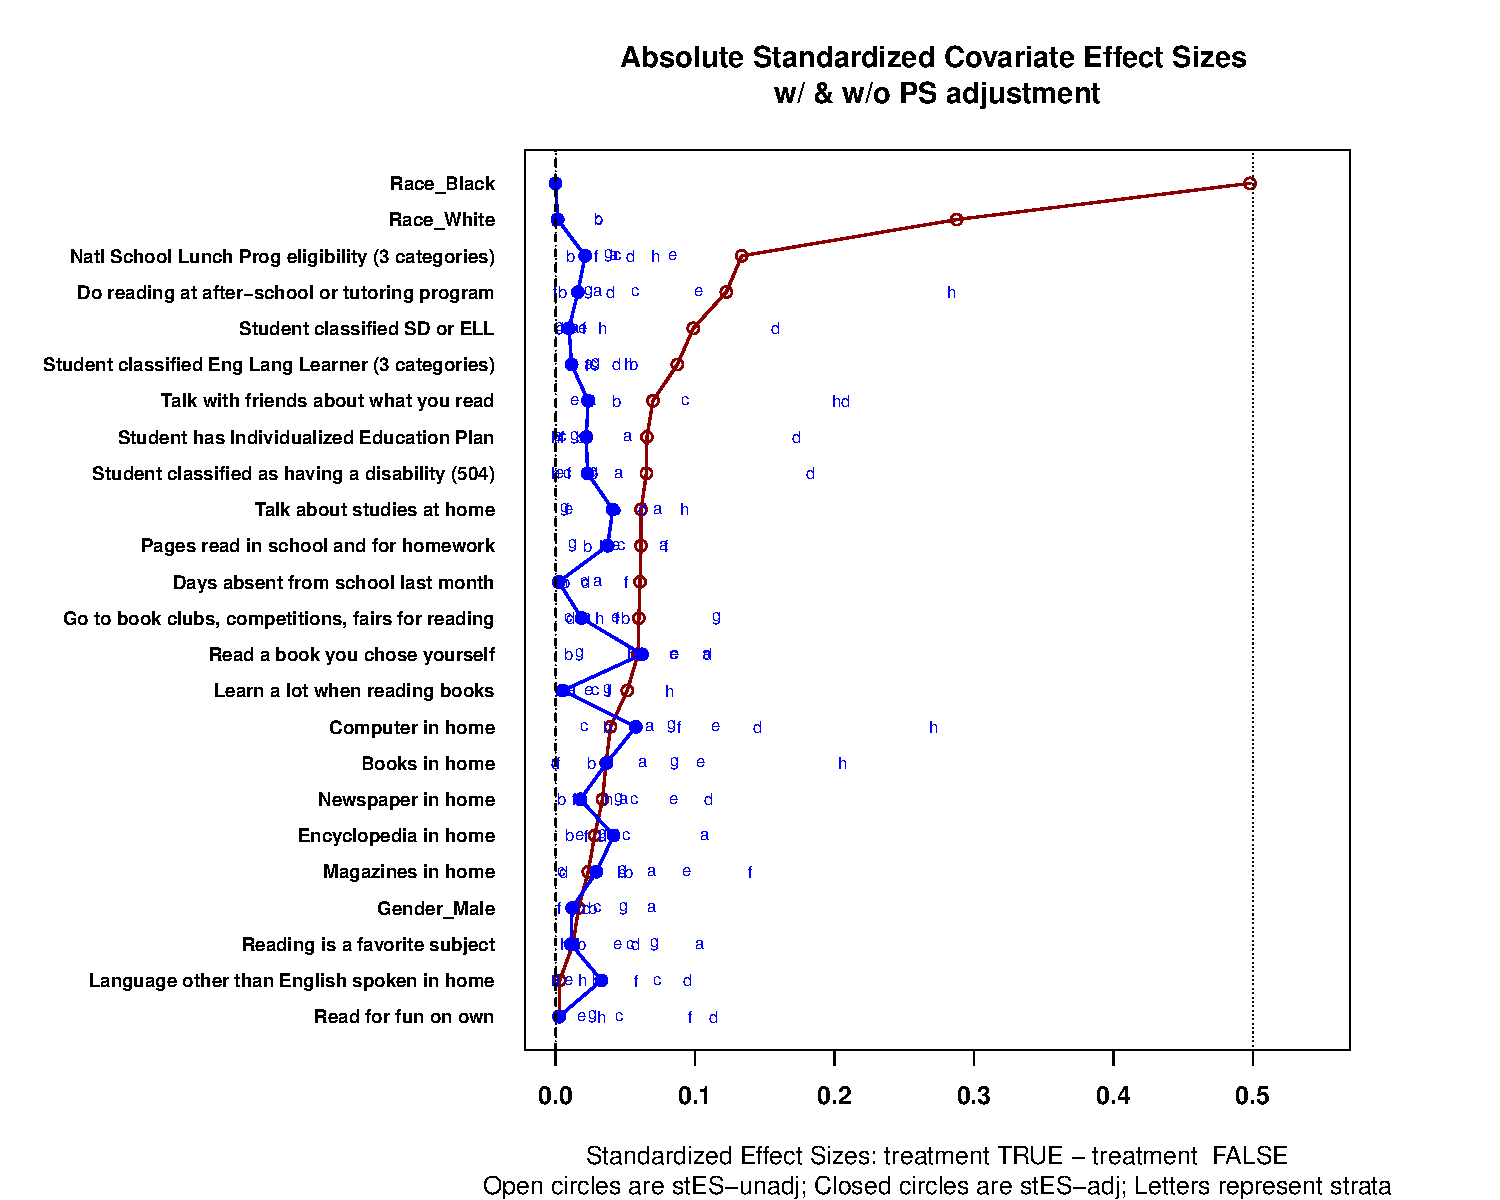
\includegraphics[width=\textwidth]{../Figures2009/g4read-tree-balance.pdf}
\caption{Covariate balance plot for classification tree stratification: Grade 4 reading}
\end{center}
\end{figure}

% Grade 8 math
\begin{figure}[h!]
\begin{center}
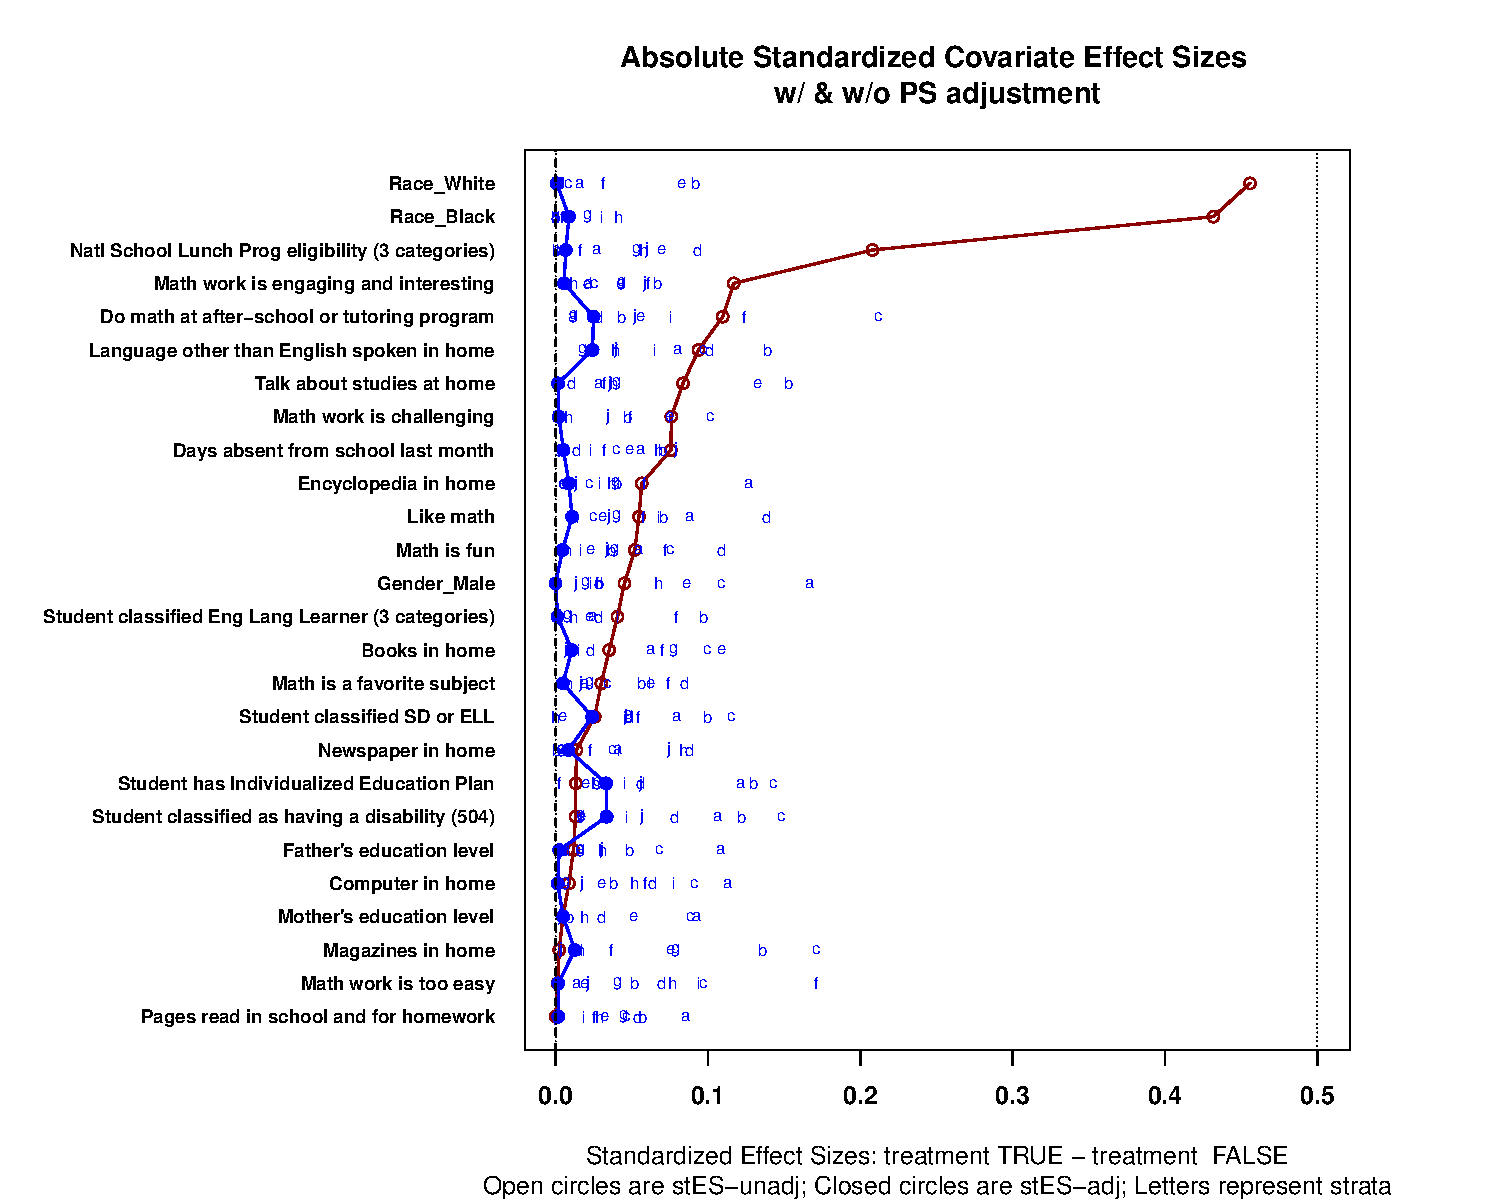
\includegraphics[width=\textwidth]{../Figures2009/g8math-lr-balance.pdf}
\caption{Covariate balance plot for logistic regression stratification: Grade 8 math}
\end{center}
\end{figure}

\begin{figure}
\begin{center}
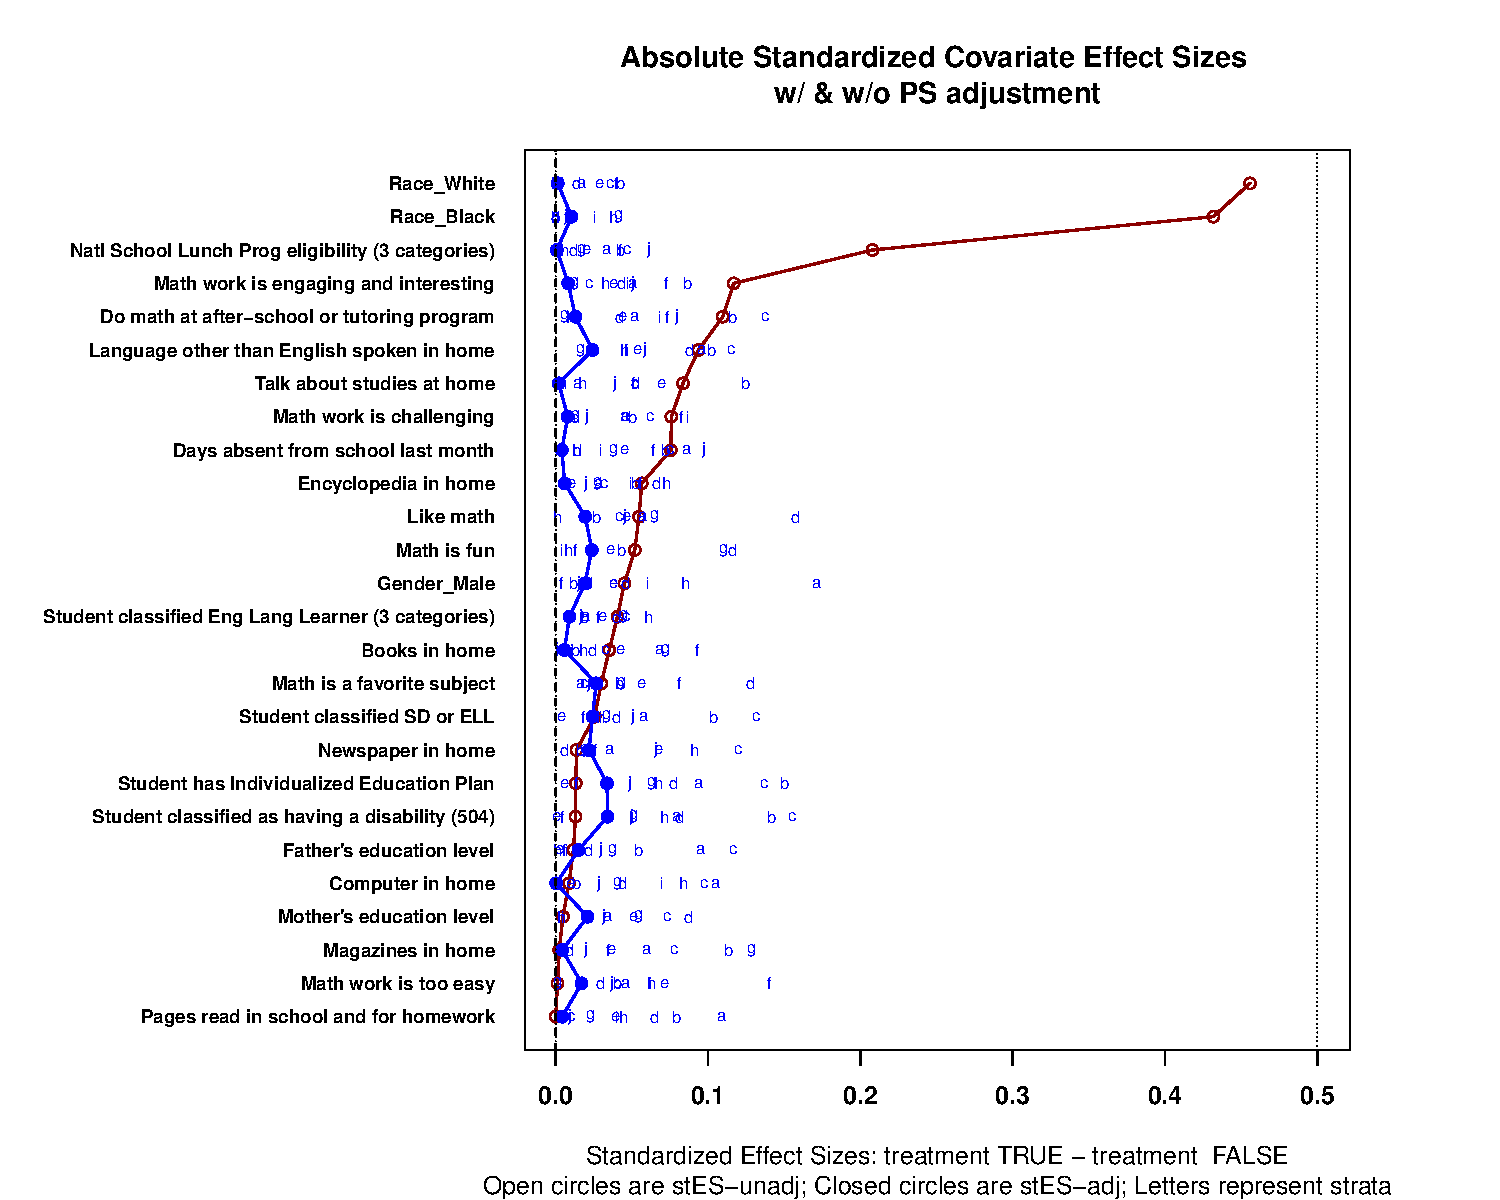
\includegraphics[width=\textwidth]{../Figures2009/g8math-lrAIC-balance.pdf}
\caption{Covariate balance plot for logistic regression AIC stratification: Grade 8 math}
\end{center}
\end{figure}

\begin{figure}
\begin{center}
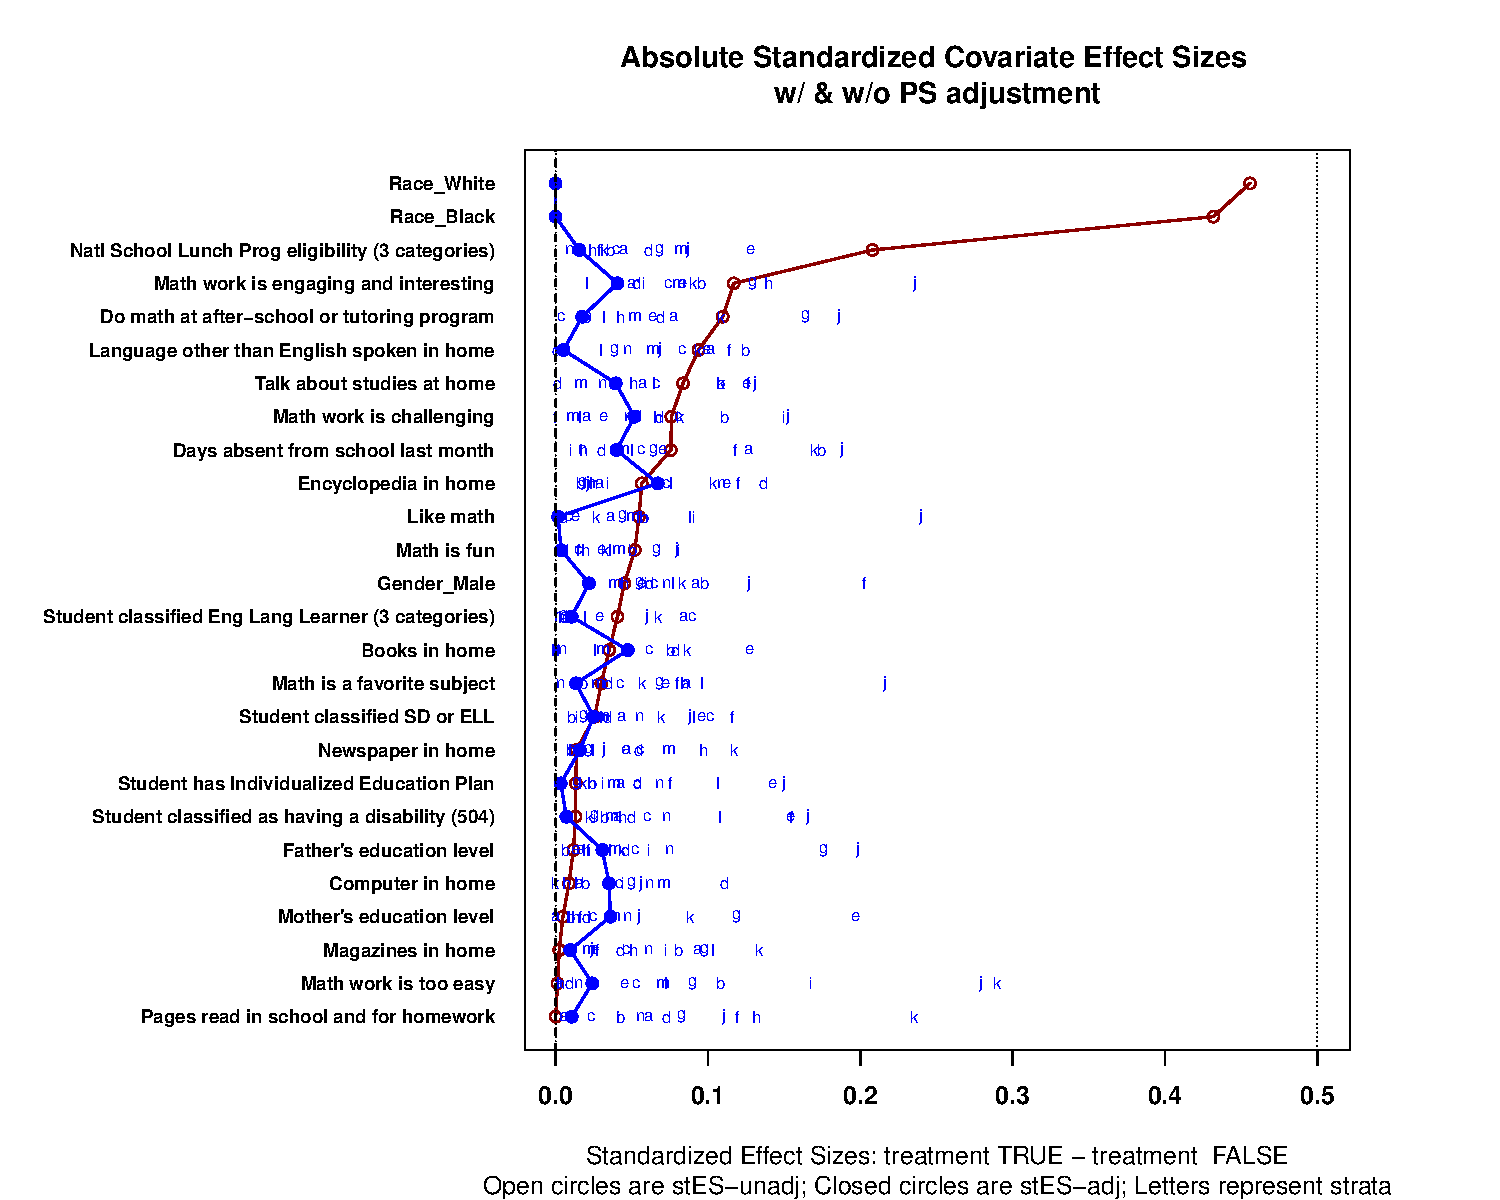
\includegraphics[width=\textwidth]{../Figures2009/g8math-tree-balance.pdf}
\caption{Covariate balance plot for classification tree stratification: Grade 8 math}
\end{center}
\end{figure}

% Grade 8 reading
\begin{figure}[h!]
\begin{center}
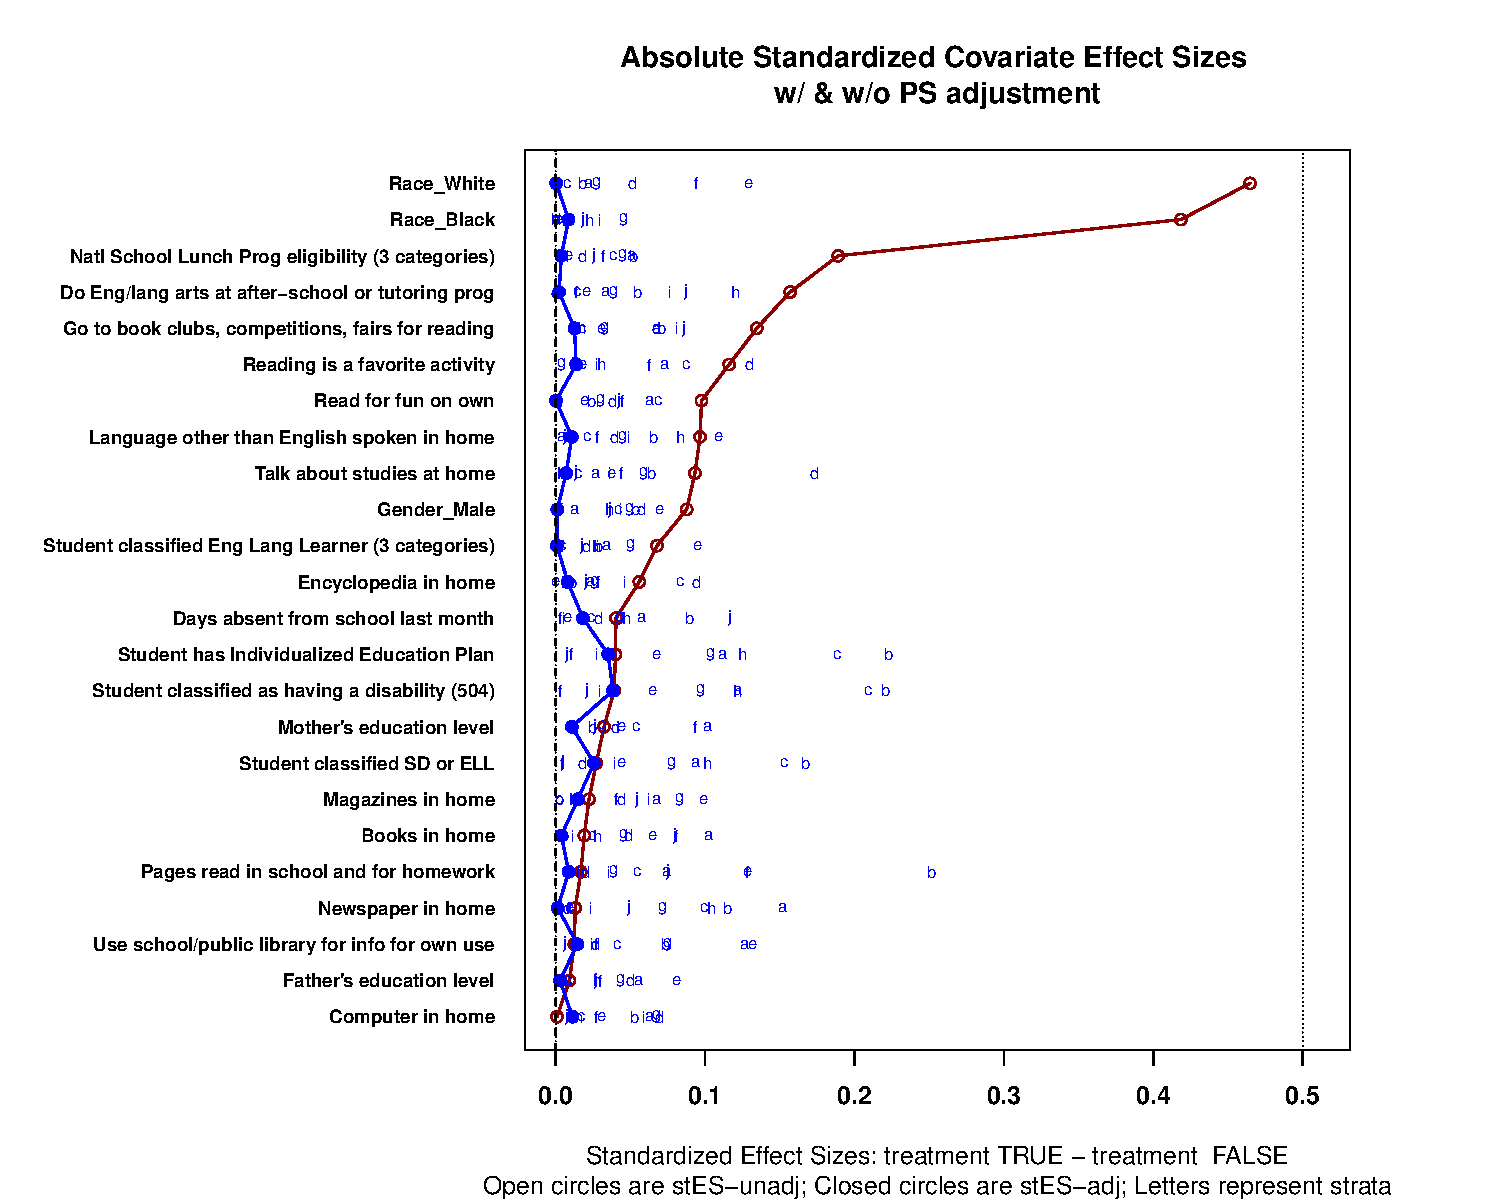
\includegraphics[width=\textwidth]{../Figures2009/g8read-lr-balance.pdf}
\caption{Covariate balance plot for logistic regression stratification: Grade 8 reading}
\end{center}
\end{figure}

\begin{figure}
\begin{center}
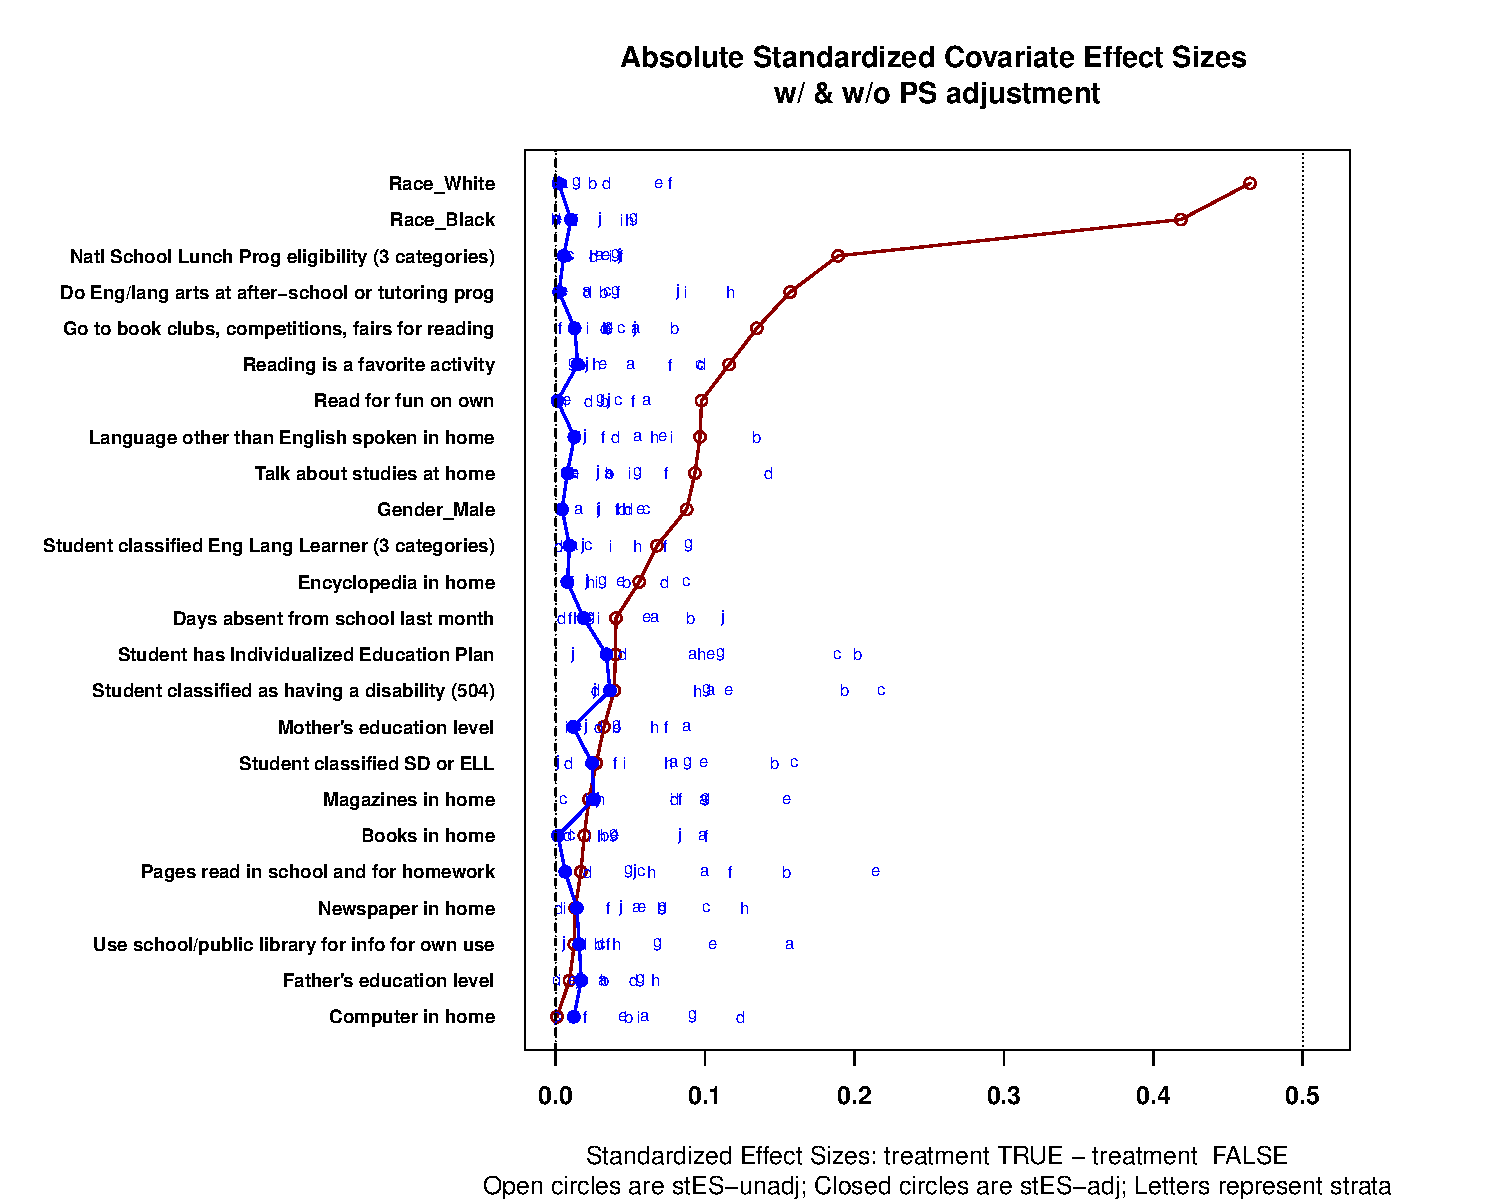
\includegraphics[width=\textwidth]{../Figures2009/g8read-lrAIC-balance.pdf}
\caption{Covariate balance plot for logistic regression AIC stratification: Grade 8 reading}
\end{center}
\end{figure}

\begin{figure}
\begin{center}
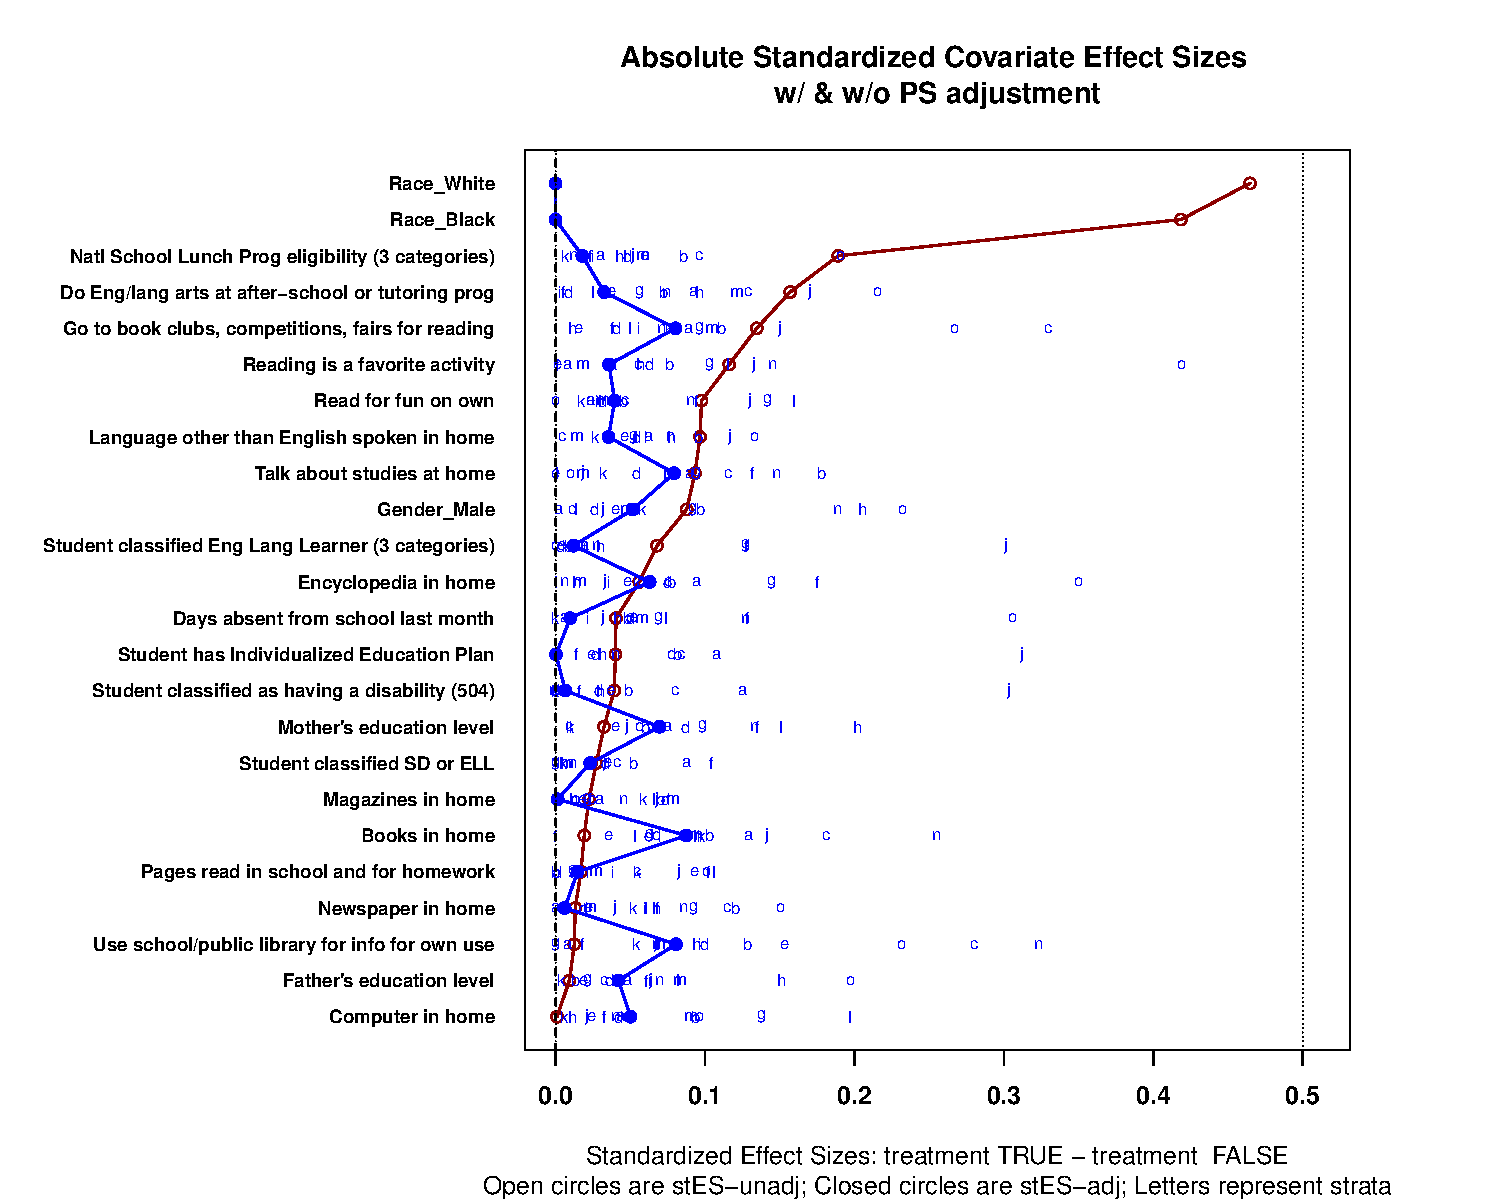
\includegraphics[width=\textwidth]{../Figures2009/g8read-tree-balance.pdf}
\caption{Covariate balance plot for classification tree stratification: Grade 8 reading}
\end{center}
\end{figure}

%==================== Appendix F ====================================================================
\clearpage
\addcontentsline{toc}{subsection}{Appendix F: Classification Method Results}
\section*{Appendix F\\Classification Method Results}
\label{appendixF}

% Grade 4 reading
\begin{figure}[h!]
\begin{center}
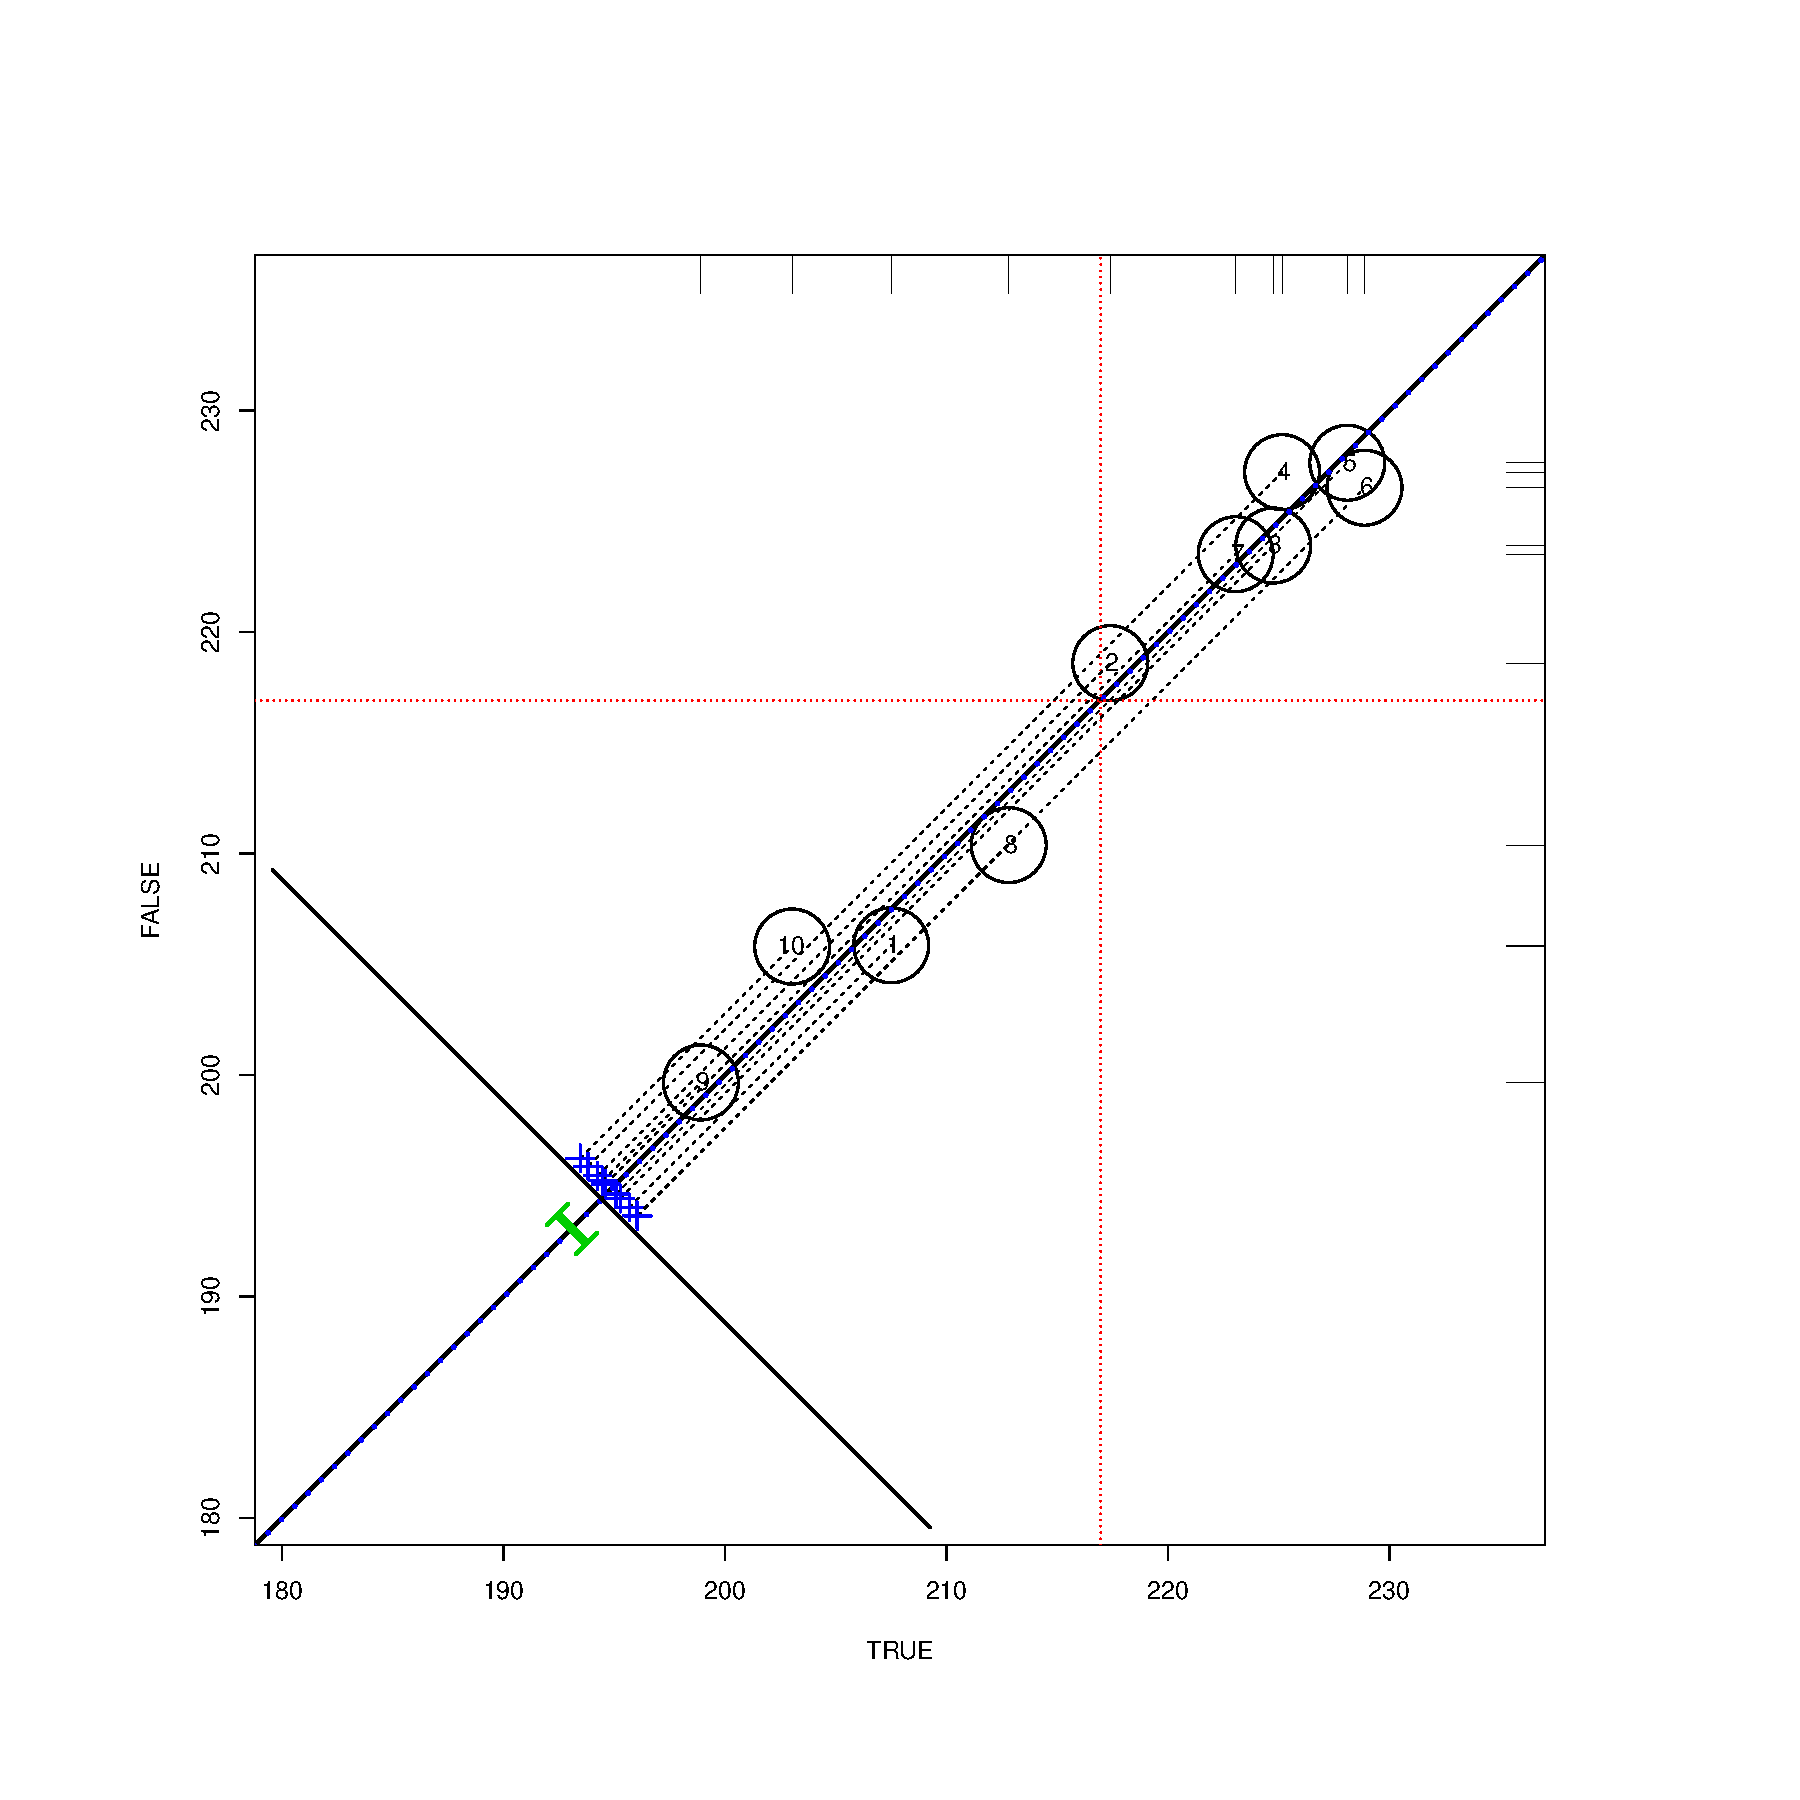
\includegraphics[height=.4\textheight,width=.4\textheight]{../Figures2009/g4read-circpsa10.pdf}
\caption{Propensity score assessment plot for logistic regression stratification: Grade 4 reading}
\end{center}
\end{figure}

% latex table generated in R 3.0.2 by xtable 1.7-1 package
% Sun Feb 23 12:17:36 2014
{\normalsize
\begin{table}[h!]
\centering
\caption{Logistic regression stratification results for grade 4 reading} 
\label{g4read-circpsa10}
\begin{tabular}{lrr@{\extracolsep{.2cm}}rr}
  \hline
   & \multicolumn{2}{c}{Public} & \multicolumn{2}{c}{Charter} \\ \cline{2-3} \cline{4-5} Strata & Mean & n & Mean & n \\ \hline
1 & 205.86 & 9440 & 207.51 & 201 \\ 
  2 & 218.60 & 9396 & 217.40 & 244 \\ 
  3 & 223.91 & 9439 & 224.76 & 202 \\ 
  4 & 227.23 & 9403 & 225.16 & 236 \\ 
  5 & 227.65 & 9371 & 228.10 & 270 \\ 
  6 & 226.52 & 9334 & 228.88 & 306 \\ 
  7 & 223.52 & 9317 & 223.07 & 323 \\ 
  8 & 210.39 & 9292 & 212.81 & 348 \\ 
  9 & 199.67 & 8990 & 198.92 & 650 \\ 
  10 & 205.81 & 8774 & 203.04 & 867 \\ 
   \hline
\end{tabular}
\end{table}
}


\clearpage

\begin{figure}
\begin{center}
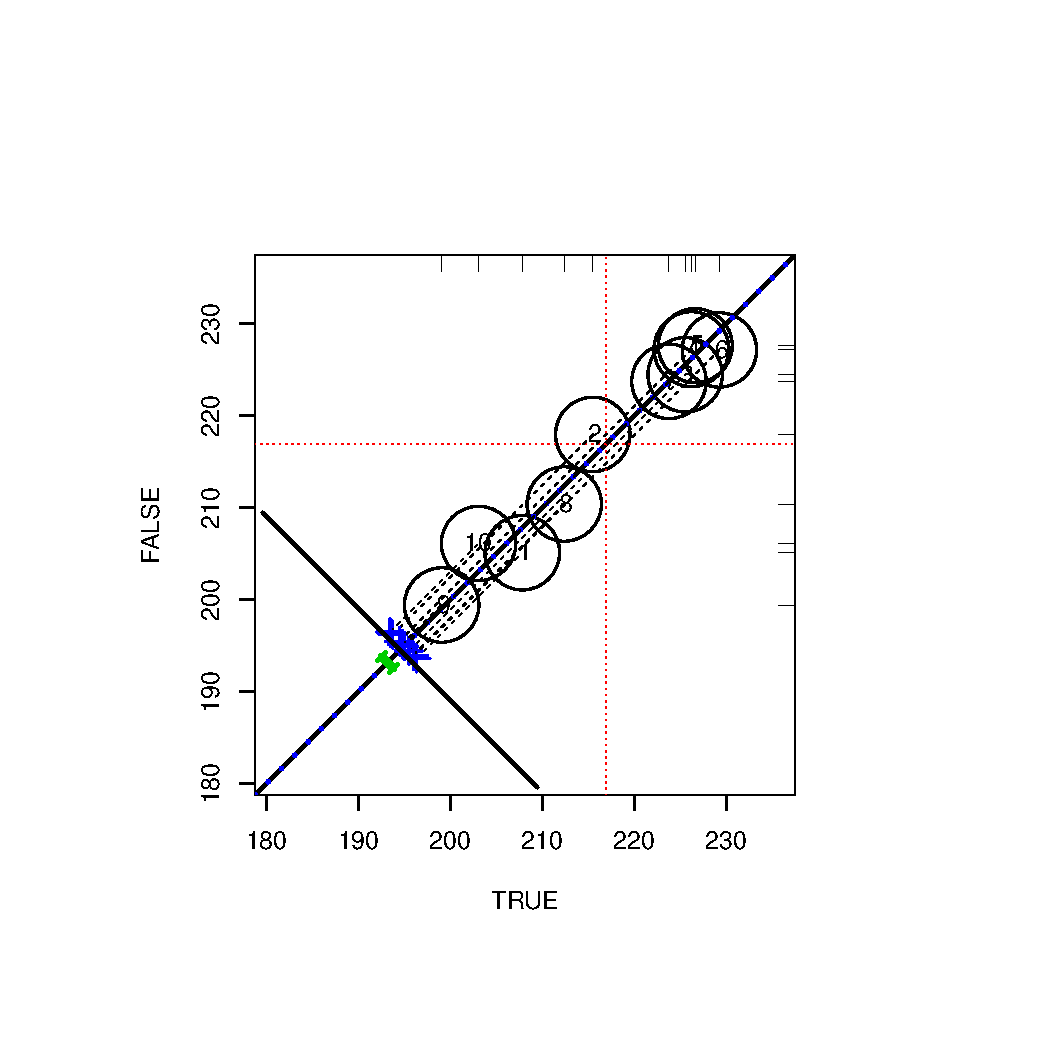
\includegraphics[height=.4\textheight,width=.4\textheight]{../Figures2009/g4read-circpsa10-AIC.pdf}
\caption{Propensity score assessment plot for logistic regression AIC stratification: Grade 4 reading}
\end{center}
\end{figure}

% latex table generated in R 3.0.2 by xtable 1.7-1 package
% Sun Feb 23 12:17:36 2014
\begin{table}[h!]
\centering
\caption{Logistic regression AIC stratification results for grade 4 reading} 
\label{g4read-circpsa10AIC}
\begin{tabular}{lrr@{\extracolsep{.2cm}}rr}
  \hline
   & \multicolumn{2}{c}{Public} & \multicolumn{2}{c}{Charter} \\ \cline{2-3} \cline{4-5} Strata & Mean & n & Mean & n \\ \hline
1 & 205.11 & 9434 & 207.83 & 218 \\ 
  2 & 217.96 & 9415 & 215.48 & 215 \\ 
  3 & 224.45 & 9406 & 225.53 & 233 \\ 
  4 & 227.24 & 9562 & 226.22 & 230 \\ 
  5 & 227.62 & 9241 & 226.63 & 263 \\ 
  6 & 227.15 & 9341 & 229.26 & 284 \\ 
  7 & 223.73 & 9296 & 223.77 & 354 \\ 
  8 & 210.40 & 9293 & 212.38 & 337 \\ 
  9 & 199.42 & 8996 & 199.06 & 648 \\ 
  10 & 206.10 & 8772 & 203.07 & 865 \\ 
   \hline
\end{tabular}
\end{table}


\clearpage

\begin{figure}
\begin{center}
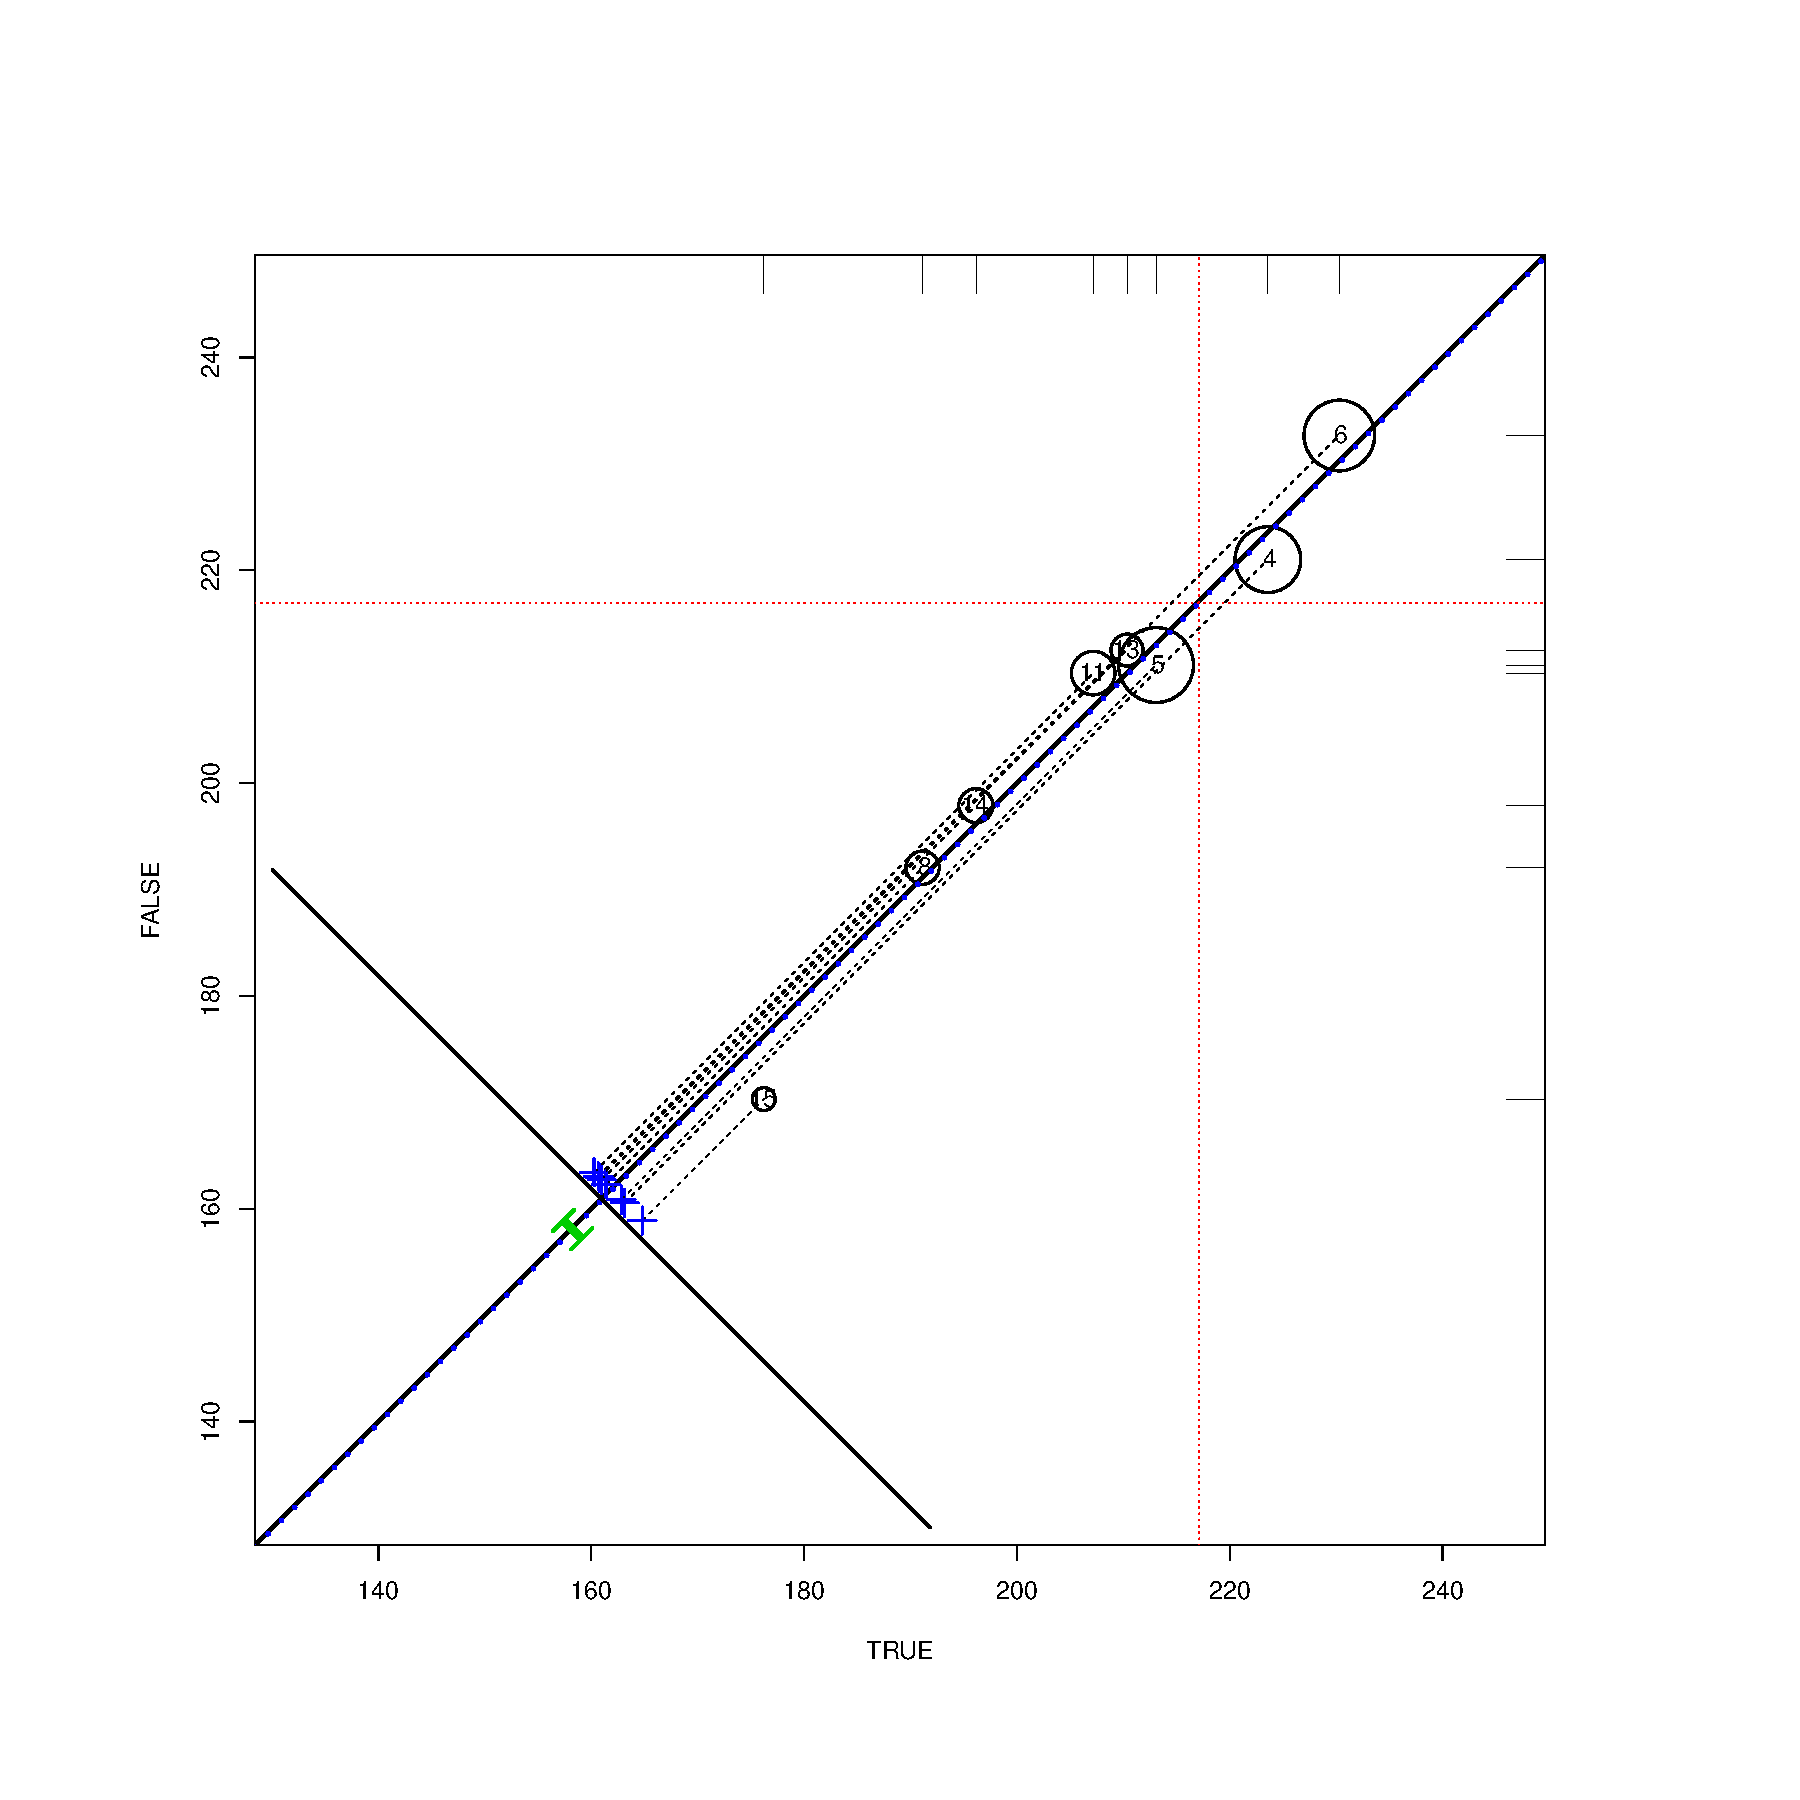
\includegraphics[height=.4\textheight,width=.4\textheight]{../Figures2009/g4read-circpsa-tree.pdf}
\caption{Propensity score assessment plot for classification tree stratification: Grade 4 reading}
\end{center}
\end{figure}

% latex table generated in R 3.0.2 by xtable 1.7-1 package
% Sun Feb 23 12:17:36 2014
\begin{table}[ht]
\centering
\caption{Classification Trees Stratification Results for Grade 4 read} 
\label{g4read-circpsa-tree}
\begin{tabular}{lrr@{\extracolsep{.2cm}}rr}
  \hline
   & \multicolumn{2}{c}{Public} & \multicolumn{2}{c}{Charter} \\ \cline{2-3} \cline{4-5} Strata & Mean & n & Mean & n \\ \hline
4 & 220.99 & 20677 & 223.57 & 464 \\ 
  5 & 211.08 & 28477 & 213.06 & 826 \\ 
  6 & 232.65 & 24503 & 230.28 & 785 \\ 
  8 & 192.06 & 3690 & 191.14 & 223 \\ 
  11 & 210.33 & 7001 & 207.16 & 547 \\ 
  13 & 212.50 & 3225 & 210.35 & 294 \\ 
  14 & 197.88 & 3735 & 196.15 & 429 \\ 
  15 & 170.31 & 1448 & 176.22 &  79 \\ 
   \hline
\end{tabular}
\end{table}


% Grade 8 math
\begin{figure}[h!]
\begin{center}
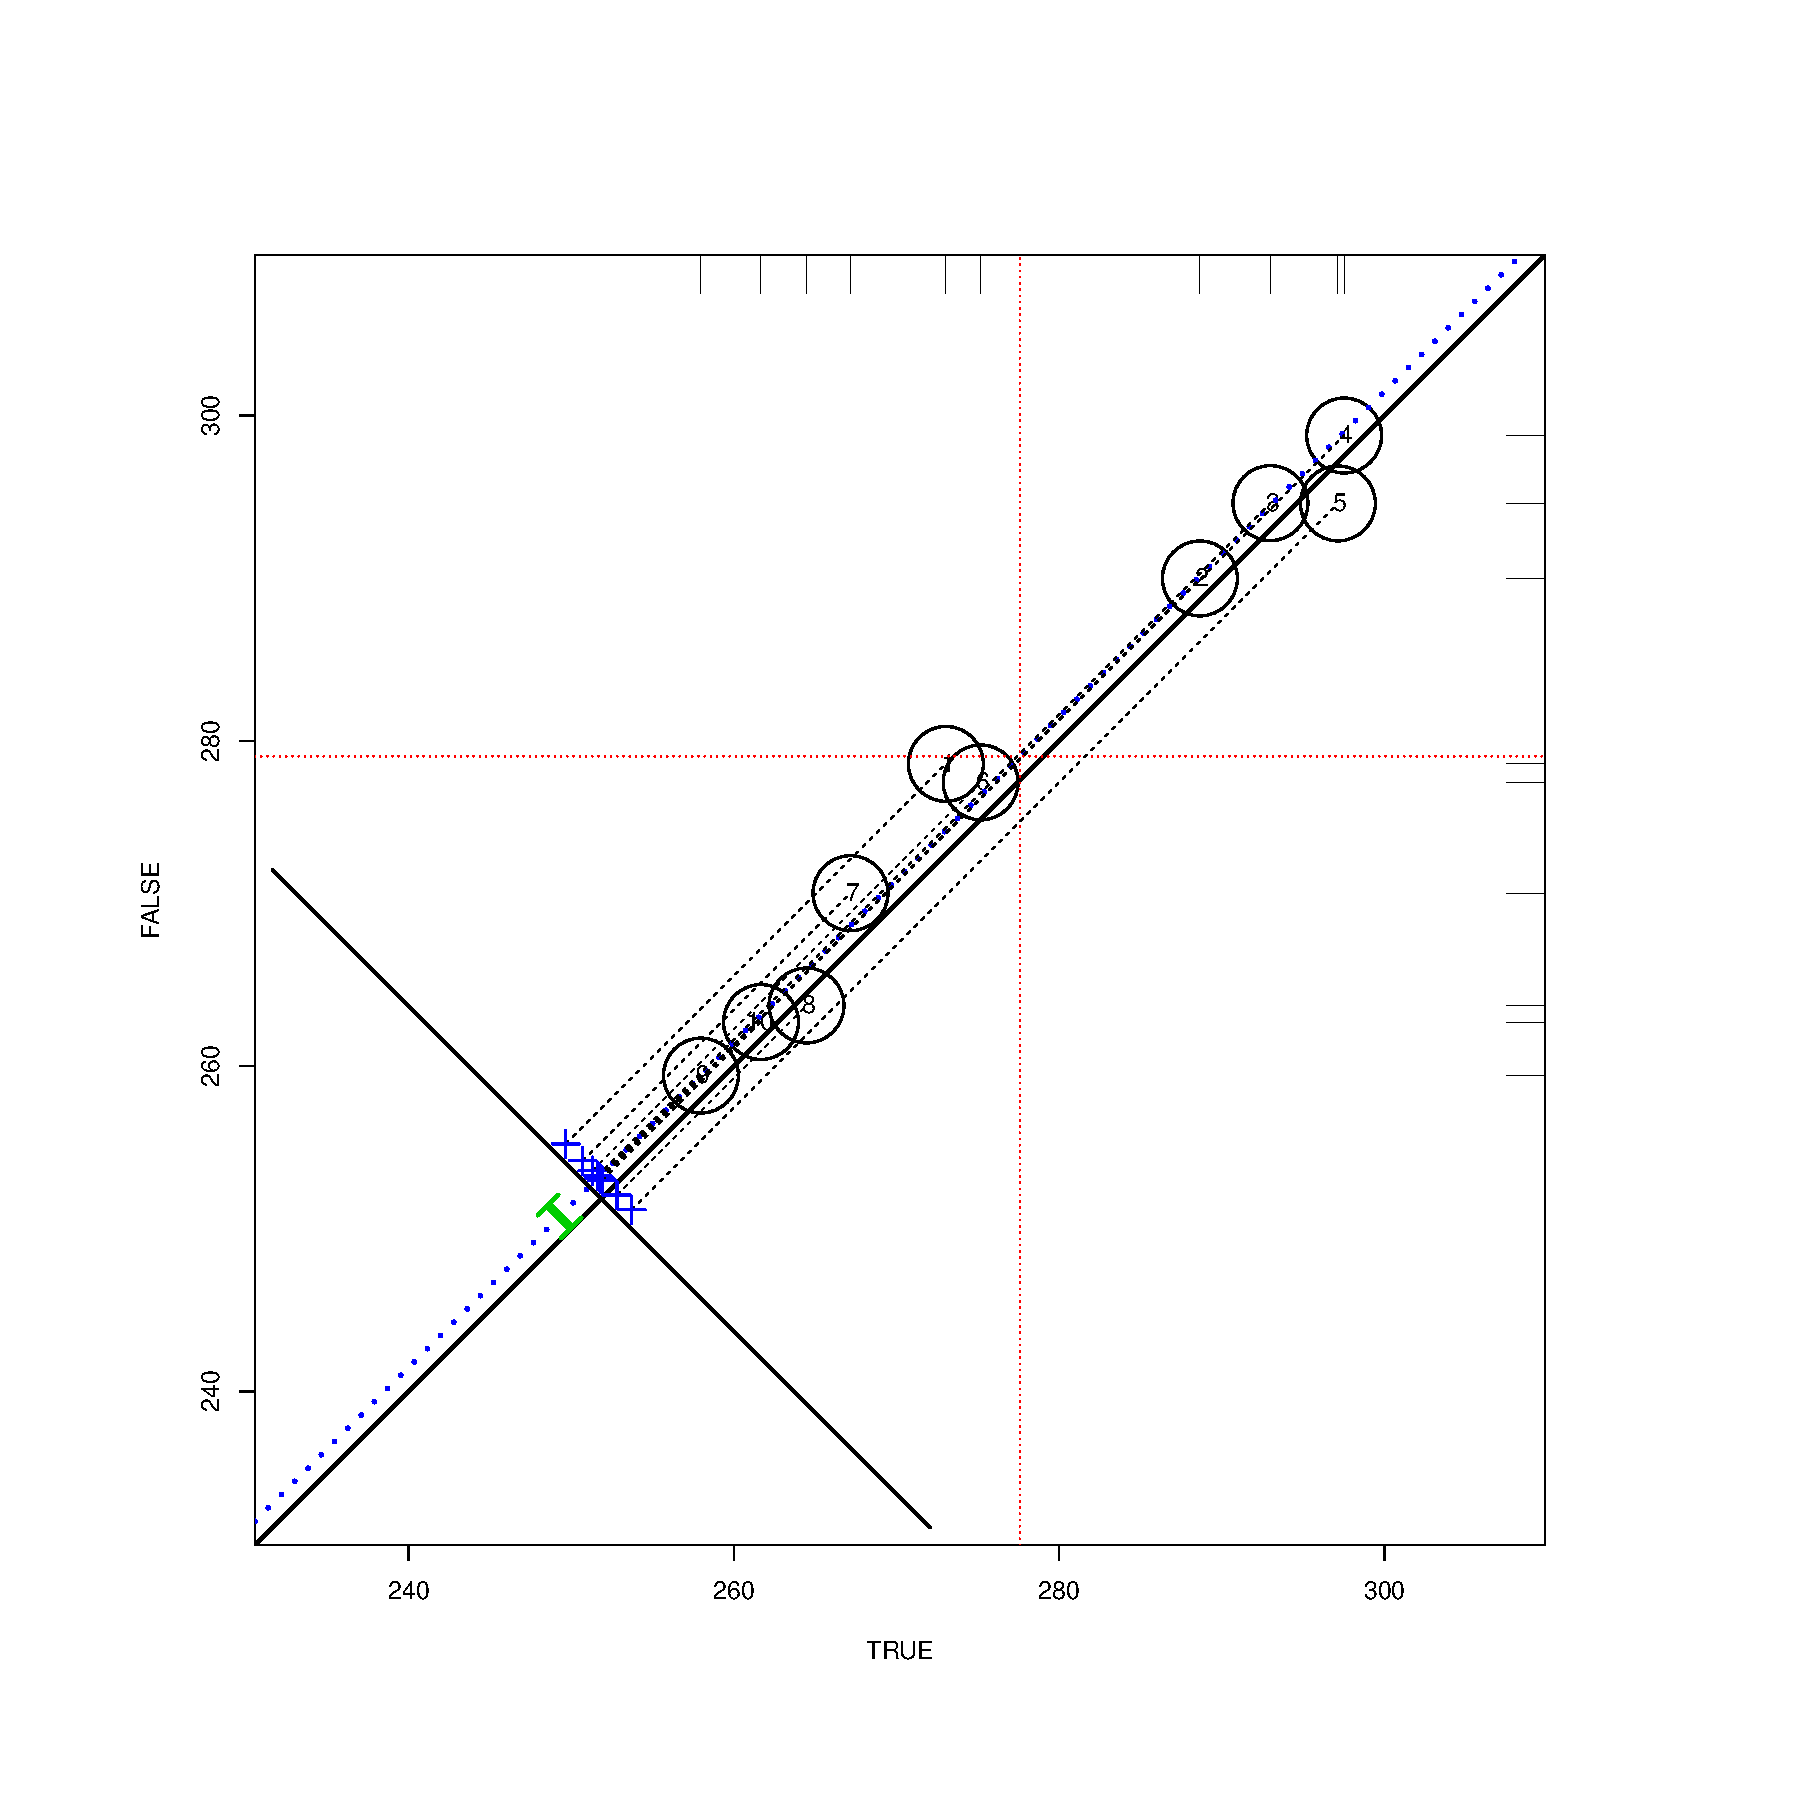
\includegraphics[height=.4\textheight,width=.4\textheight]{../Figures2009/g8math-circpsa10.pdf}
\caption{Propensity score assessment plot for logistic regression stratification: Grade 8 math}
\end{center}
\end{figure}

% latex table generated in R 3.0.1 by xtable 1.7-1 package
% Thu Jun 20 13:40:46 2013
\begin{table}[ht]
\centering
\caption{Logistic Regression Stratification Results for Grade 8 math} 
\label{g8math-circpsa10}
\begin{tabular}{lrr@{\extracolsep{.2cm}}rr}
  \hline
   & \multicolumn{2}{c}{Public} & \multicolumn{2}{c}{Charter} \\ \cline{2-3} \cline{4-5} Strata & Mean & n & Mean & n \\ \hline
1 & 278.58 & 7402 & 273.03 & 135 \\ 
  2 & 289.98 & 7359 & 288.65 & 177 \\ 
  3 & 294.62 & 7334 & 292.99 & 202 \\ 
  4 & 298.77 & 7292 & 297.52 & 244 \\ 
  5 & 294.60 & 7207 & 297.14 & 329 \\ 
  6 & 277.44 & 7183 & 275.17 & 353 \\ 
  7 & 270.63 & 7132 & 267.17 & 404 \\ 
  8 & 263.73 & 7022 & 264.47 & 514 \\ 
  9 & 259.42 & 6864 & 257.97 & 672 \\ 
  10 & 262.71 & 6733 & 261.67 & 803 \\ 
   \hline
\end{tabular}
\end{table}


\clearpage
\begin{figure}
\begin{center}
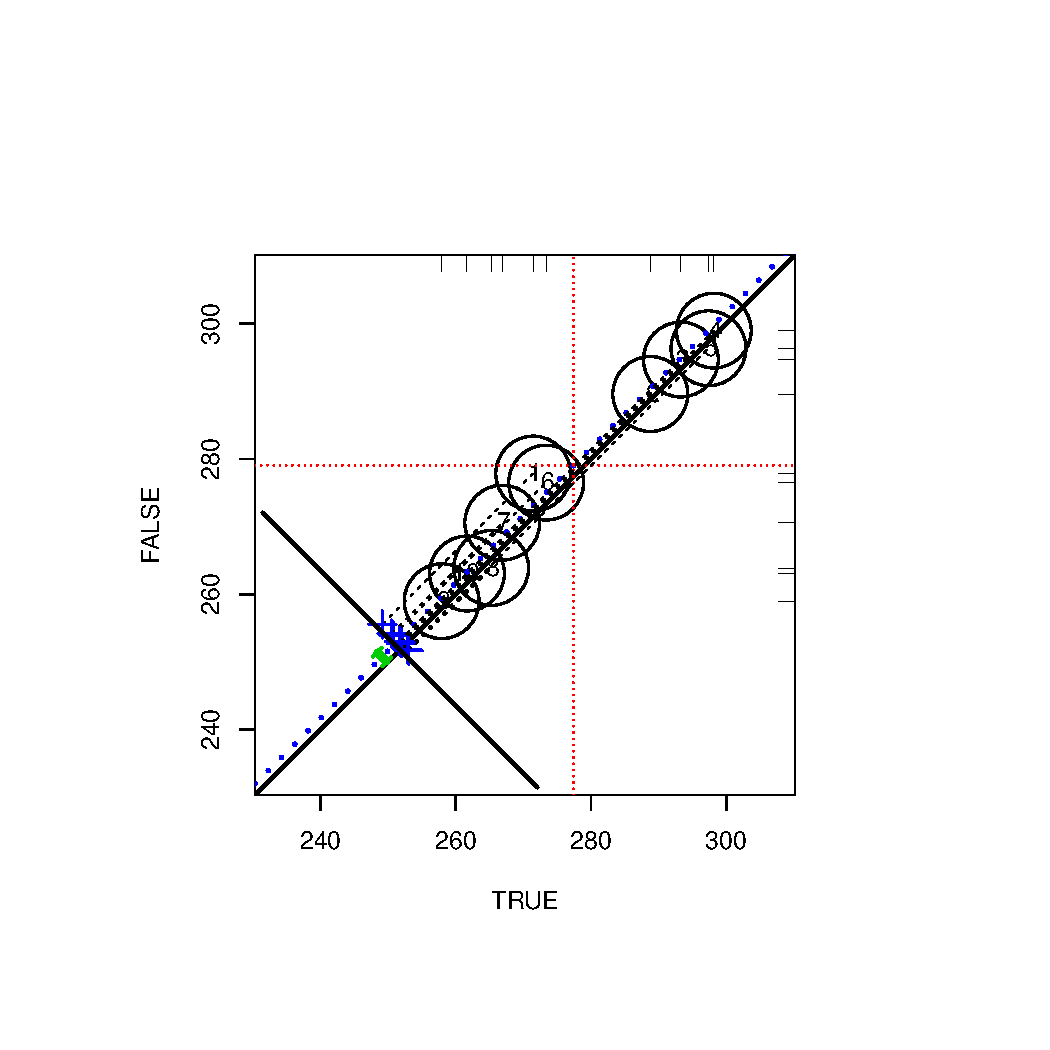
\includegraphics[height=.4\textheight,width=.4\textheight]{../Figures2009/g8math-circpsa10-AIC.pdf}
\caption{Propensity score assessment plot for logistic regression AIC stratification: Grade 8 math}
\end{center}
\end{figure}

% latex table generated in R 3.0.2 by xtable 1.7-1 package
% Sun Feb 23 12:19:00 2014
\begin{table}[ht]
\centering
\caption{Logistic regression AIC stratification results for grade 8 math} 
\label{g8math-circpsa10AIC}
\begin{tabular}{lrr@{\extracolsep{.2cm}}rr}
  \hline
   & \multicolumn{2}{c}{Public} & \multicolumn{2}{c}{Charter} \\ \cline{2-3} \cline{4-5} Strata & Mean & n & Mean & n \\ \hline
1 & 277.84 & 7407 & 271.47 & 135 \\ 
  2 & 289.62 & 7388 & 288.77 & 172 \\ 
  3 & 294.71 & 7324 & 293.29 & 211 \\ 
  4 & 299.00 & 7268 & 298.16 & 240 \\ 
  5 & 296.38 & 7199 & 297.38 & 338 \\ 
  6 & 276.51 & 7193 & 273.37 & 342 \\ 
  7 & 270.59 & 7122 & 266.88 & 417 \\ 
  8 & 263.89 & 7033 & 265.24 & 512 \\ 
  9 & 258.98 & 6862 & 257.92 & 666 \\ 
  10 & 263.08 & 6732 & 261.66 & 800 \\ 
   \hline
\end{tabular}
\end{table}


\clearpage
\begin{figure}
\begin{center}
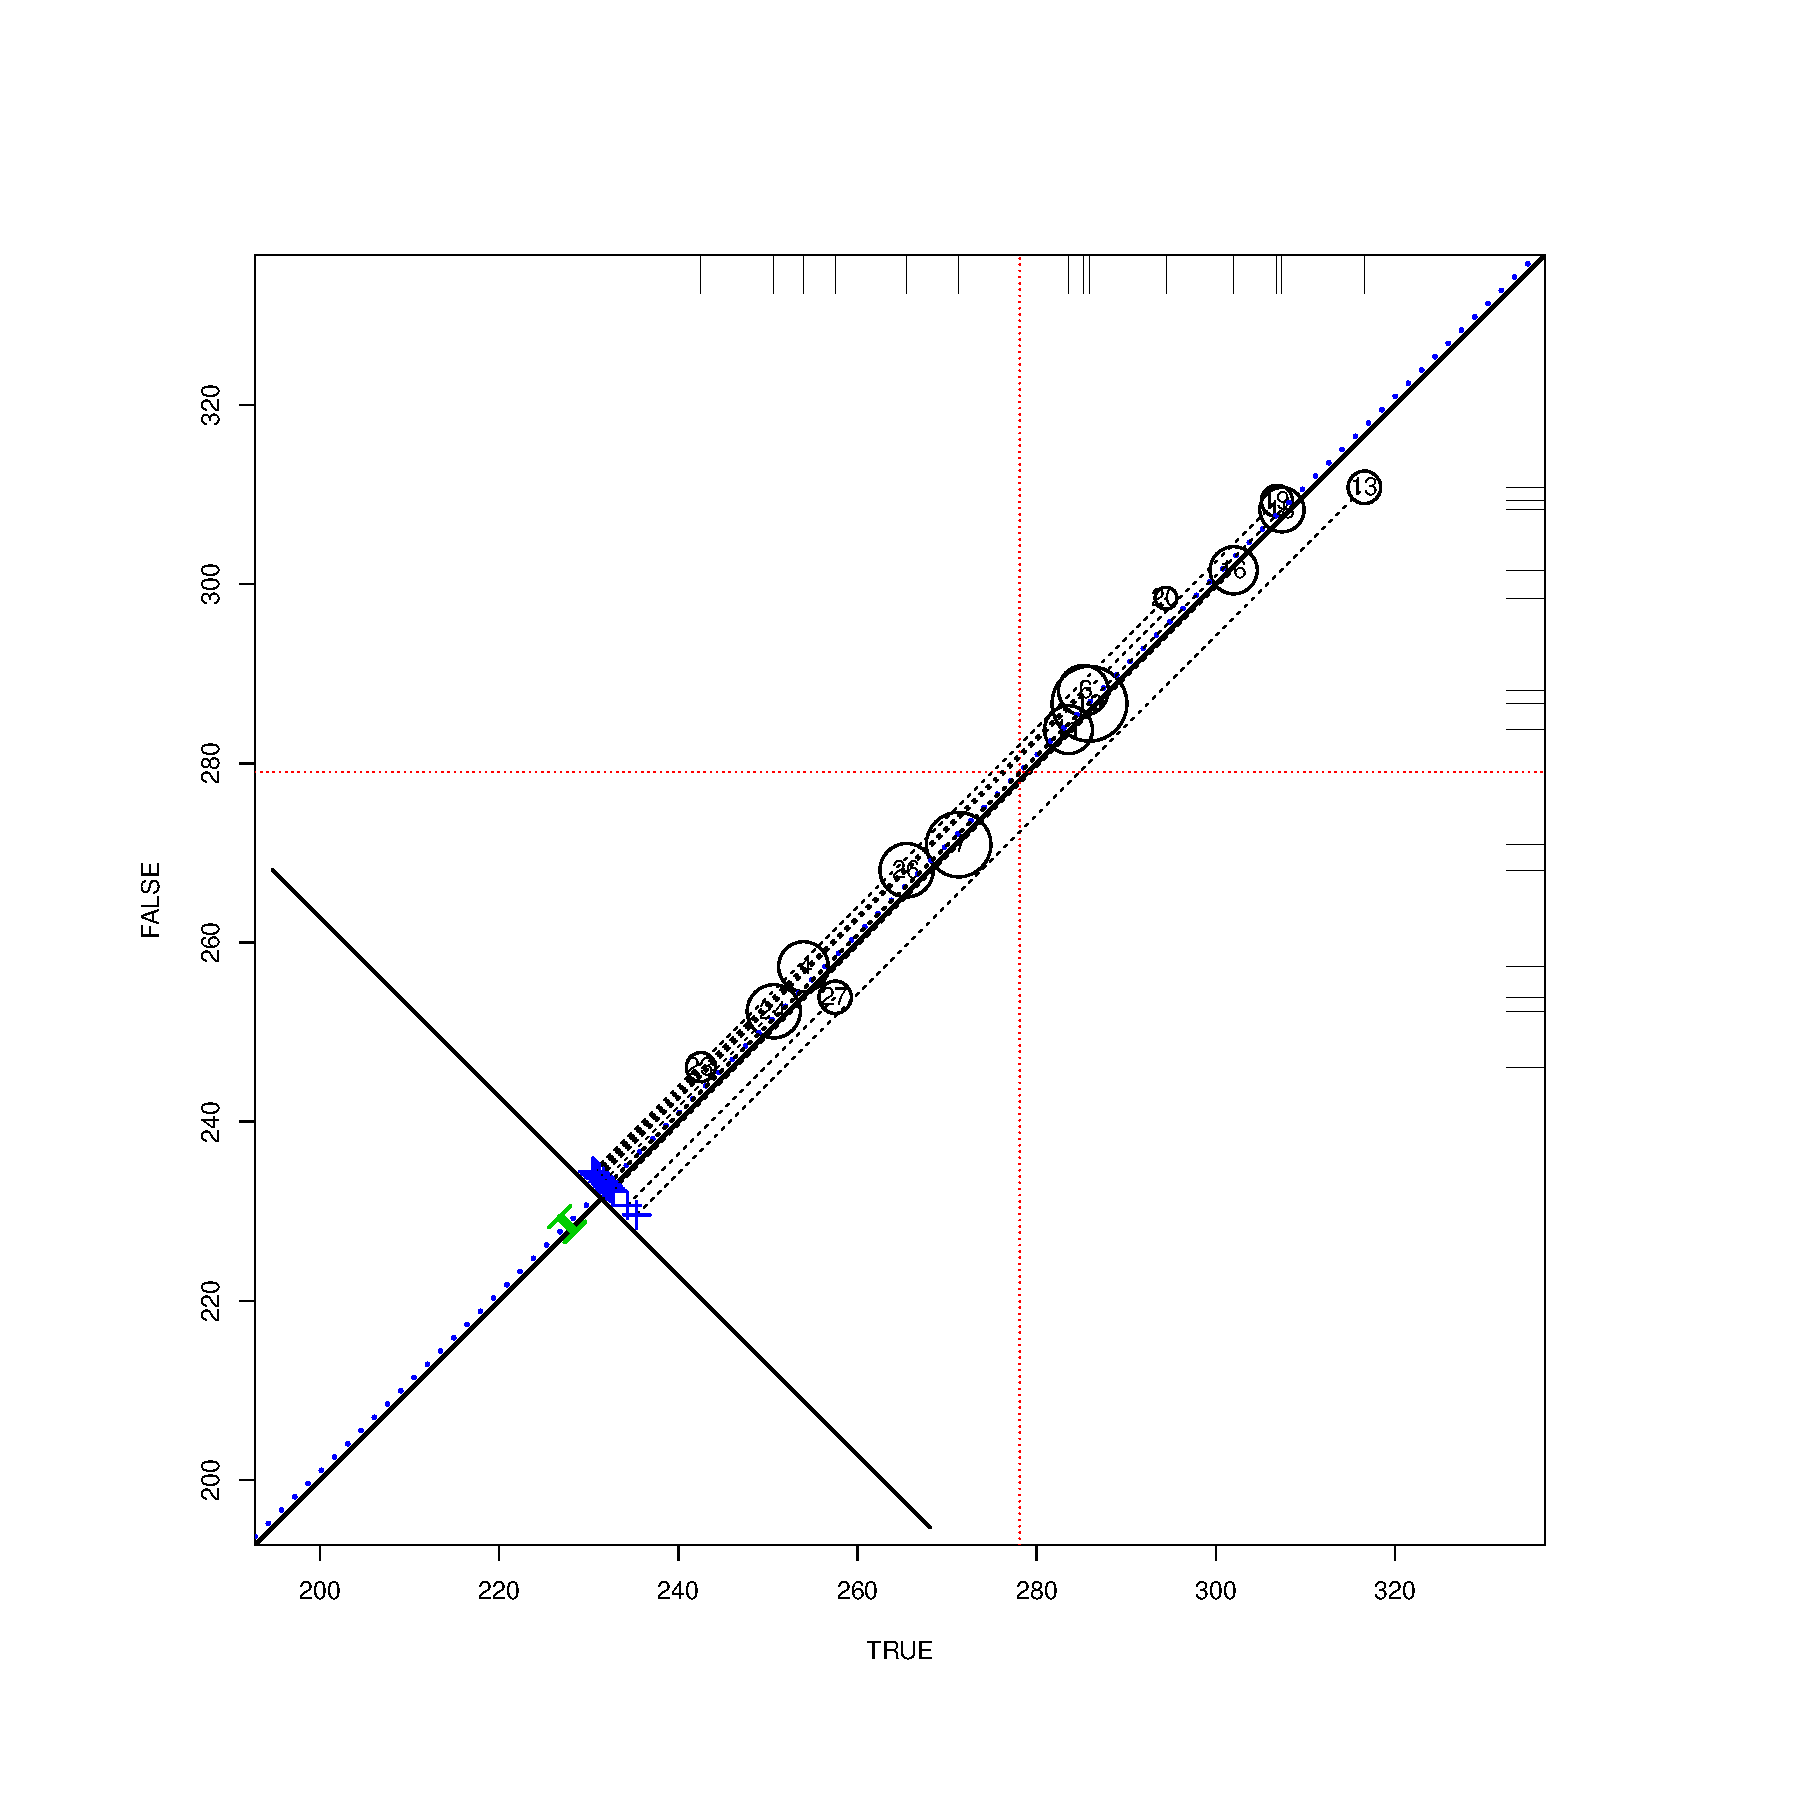
\includegraphics[height=.4\textheight,width=.4\textheight]{../Figures2009/g8math-circpsa-tree.pdf}
\caption{Propensity score assessment plot for classification tree stratification: Grade 8 math}
\end{center}
\end{figure}

% latex table generated in R 3.0.2 by xtable 1.7-1 package
% Sun Feb 23 12:19:00 2014
\begin{table}[ht]
\centering
\caption{Classification Trees Stratification Results for Grade 8 math} 
\label{g8math-circpsa-tree}
\begin{tabular}{lrr@{\extracolsep{.2cm}}rr}
  \hline
   & \multicolumn{2}{c}{Public} & \multicolumn{2}{c}{Charter} \\ \cline{2-3} \cline{4-5} Strata & Mean & n & Mean & n \\ \hline
4 & 257.31 & 5529 & 253.98 & 261 \\ 
  6 & 288.14 & 5544 & 285.21 & 257 \\ 
  7 & 270.93 & 10414 & 271.28 & 704 \\ 
  10 & 286.65 & 15771 & 285.89 & 318 \\ 
  11 & 283.75 & 5109 & 283.55 & 156 \\ 
  13 & 310.81 & 2000 & 316.58 &  51 \\ 
  16 & 301.54 & 4895 & 301.98 & 166 \\ 
  18 & 308.30 & 4163 & 307.37 & 172 \\ 
  19 & 309.29 & 1720 & 306.81 & 106 \\ 
  20 & 298.44 & 694 & 294.44 &  48 \\ 
  23 & 246.10 & 1432 & 242.53 &  92 \\ 
  24 & 252.32 & 6261 & 250.66 & 581 \\ 
  26 & 268.06 & 6244 & 265.49 & 670 \\ 
  27 & 253.90 & 1752 & 257.52 & 251 \\ 
   \hline
\end{tabular}
\end{table}


% Grade 8 reading
\clearpage
\begin{figure}[h!]
\begin{center}
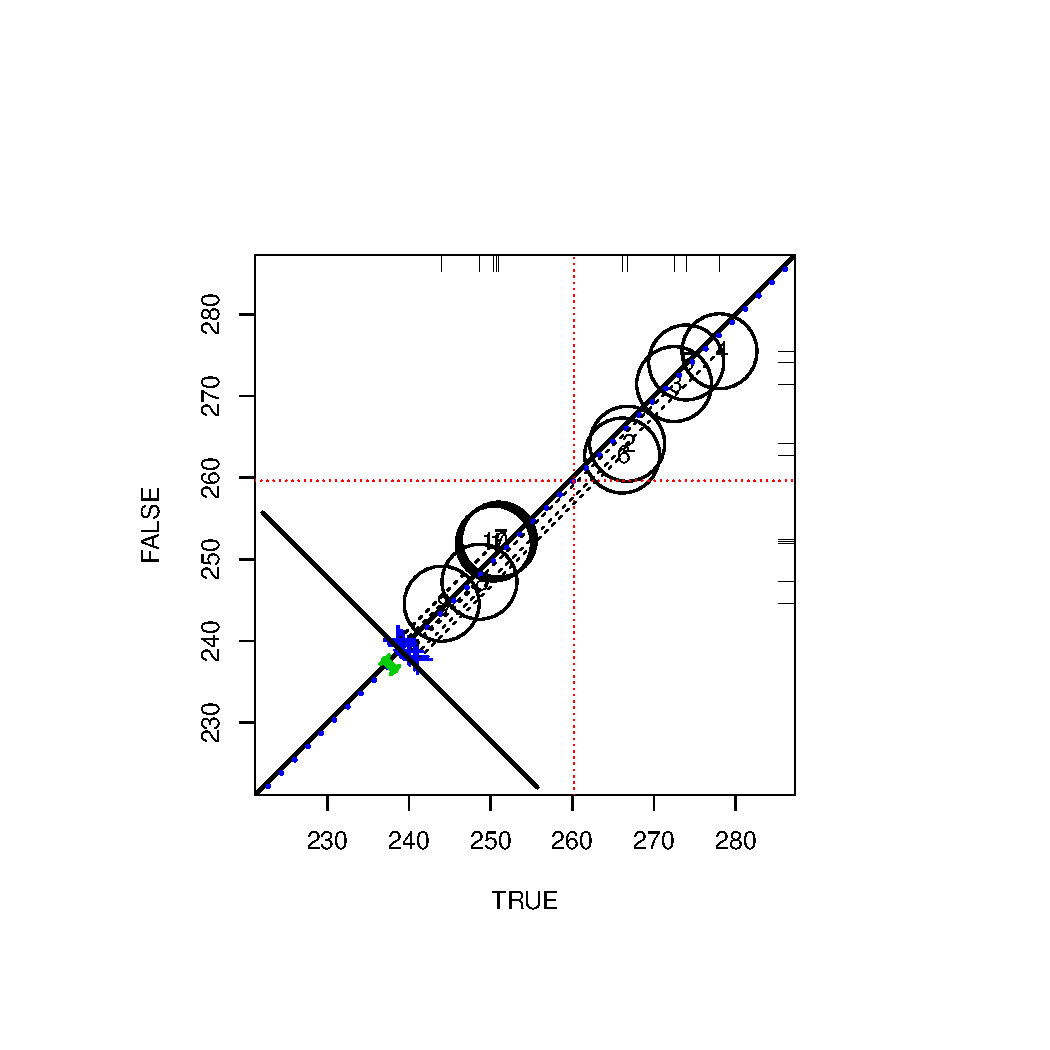
\includegraphics[height=.4\textheight,width=.4\textheight]{../Figures2009/g8read-circpsa10.pdf}
\caption{Propensity score assessment plot for logistic regression stratification: Grade 8 reading}
\end{center}
\end{figure}

% latex table generated in R 3.0.2 by xtable 1.7-1 package
% Sun Feb 23 12:20:17 2014
\begin{table}[h!]
\centering
\caption{Logistic regression stratification results for grade 8 reading} 
\label{g8read-circpsa10}
\begin{tabular}{lrr@{\extracolsep{.2cm}}rr}
  \hline
   & \multicolumn{2}{c}{Public} & \multicolumn{2}{c}{Charter} \\ \cline{2-3} \cline{4-5} Strata & Mean & n & Mean & n \\ \hline
1 & 251.94 & 7634 & 250.40 & 129 \\ 
  2 & 264.16 & 7596 & 266.72 & 167 \\ 
  3 & 271.47 & 7535 & 272.48 & 226 \\ 
  4 & 275.49 & 7519 & 278.03 & 243 \\ 
  5 & 274.12 & 7471 & 273.95 & 291 \\ 
  6 & 262.72 & 7413 & 266.11 & 349 \\ 
  7 & 252.41 & 7379 & 251.00 & 383 \\ 
  8 & 247.25 & 7213 & 248.63 & 549 \\ 
  9 & 244.57 & 7103 & 243.99 & 659 \\ 
  10 & 252.15 & 6947 & 250.66 & 816 \\ 
   \hline
\end{tabular}
\end{table}


\clearpage
\begin{figure}
\begin{center}
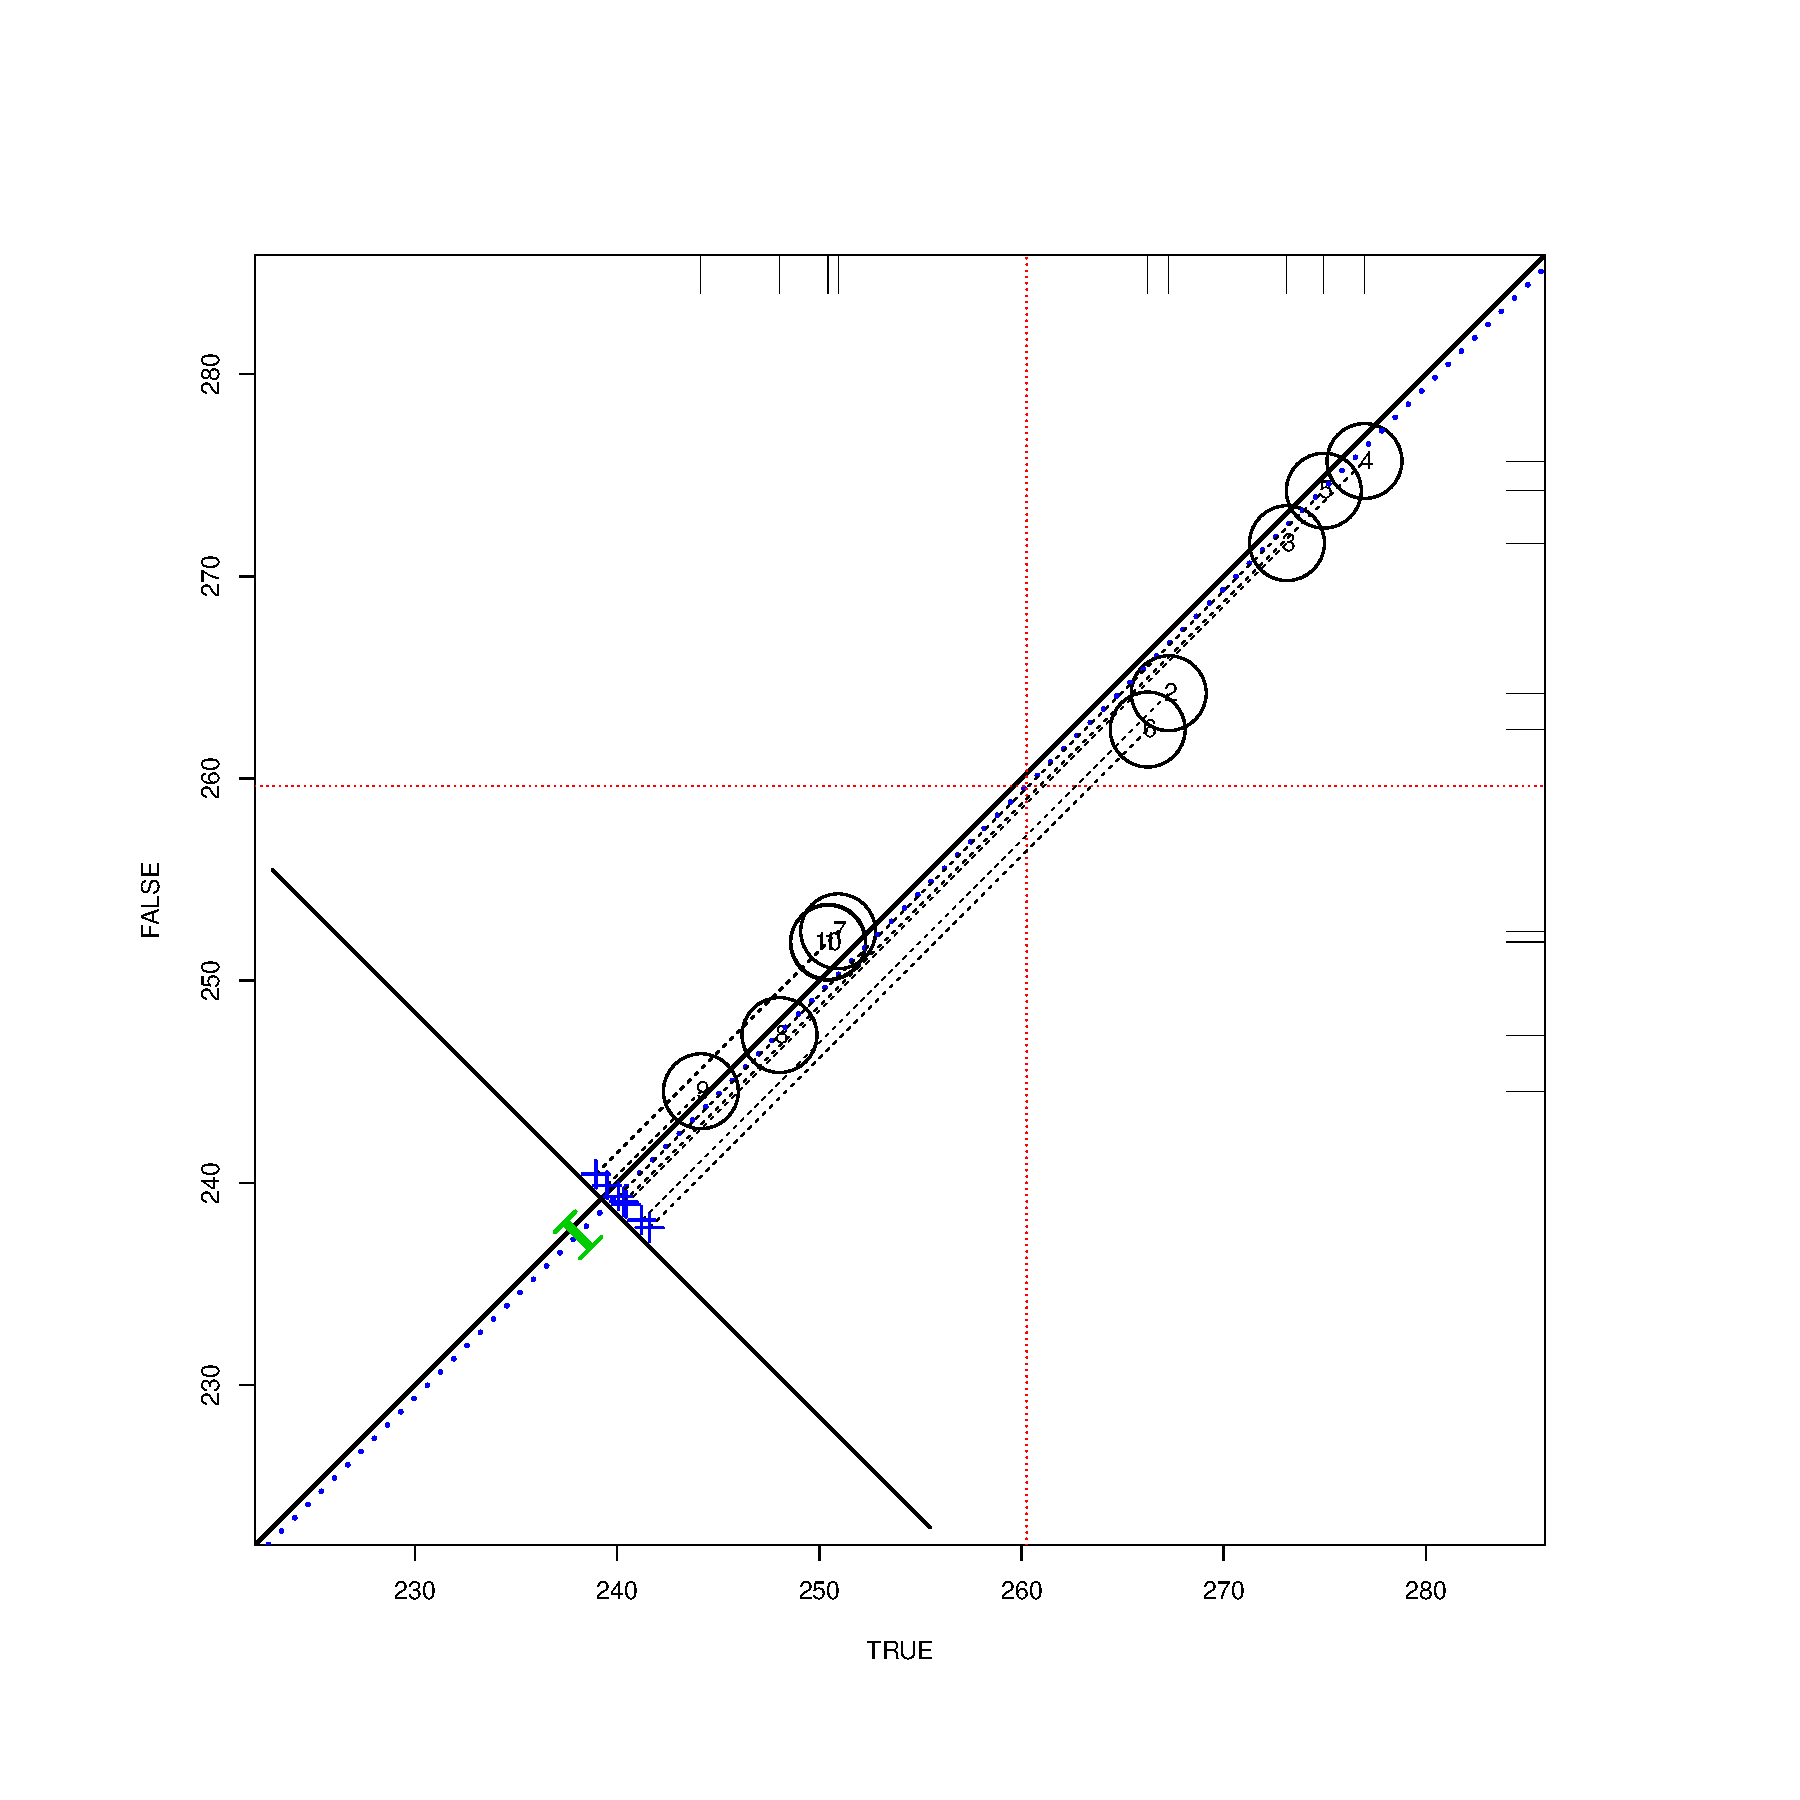
\includegraphics[height=.4\textheight,width=.4\textheight]{../Figures2009/g8read-circpsa10-AIC.pdf}
\caption{Propensity score assessment plot for logistic regression AIC stratification: Grade 8 reading}
\end{center}
\end{figure}

% latex table generated in R 3.0.2 by xtable 1.7-1 package
% Sun Feb 23 12:20:17 2014
\begin{table}[ht]
\centering
\caption{Logistic Regression AIC Stratification Results for Grade 8 read} 
\label{g8read-circpsa10AIC}
\begin{tabular}{lrr@{\extracolsep{.2cm}}rr}
  \hline
   & \multicolumn{2}{c}{Public} & \multicolumn{2}{c}{Charter} \\ \cline{2-3} \cline{4-5} Strata & Mean & n & Mean & n \\ \hline
1 & 251.87 & 7636 & 250.42 & 128 \\ 
  2 & 264.22 & 7592 & 267.28 & 169 \\ 
  3 & 271.64 & 7530 & 273.13 & 232 \\ 
  4 & 275.70 & 7530 & 276.96 & 232 \\ 
  5 & 274.23 & 7466 & 274.95 & 296 \\ 
  6 & 262.42 & 7417 & 266.24 & 345 \\ 
  7 & 252.44 & 7365 & 250.93 & 397 \\ 
  8 & 247.31 & 7208 & 248.03 & 554 \\ 
  9 & 244.53 & 7132 & 244.14 & 630 \\ 
  10 & 251.91 & 6934 & 250.44 & 829 \\ 
   \hline
\end{tabular}
\end{table}


\clearpage
\begin{figure}
\begin{center}
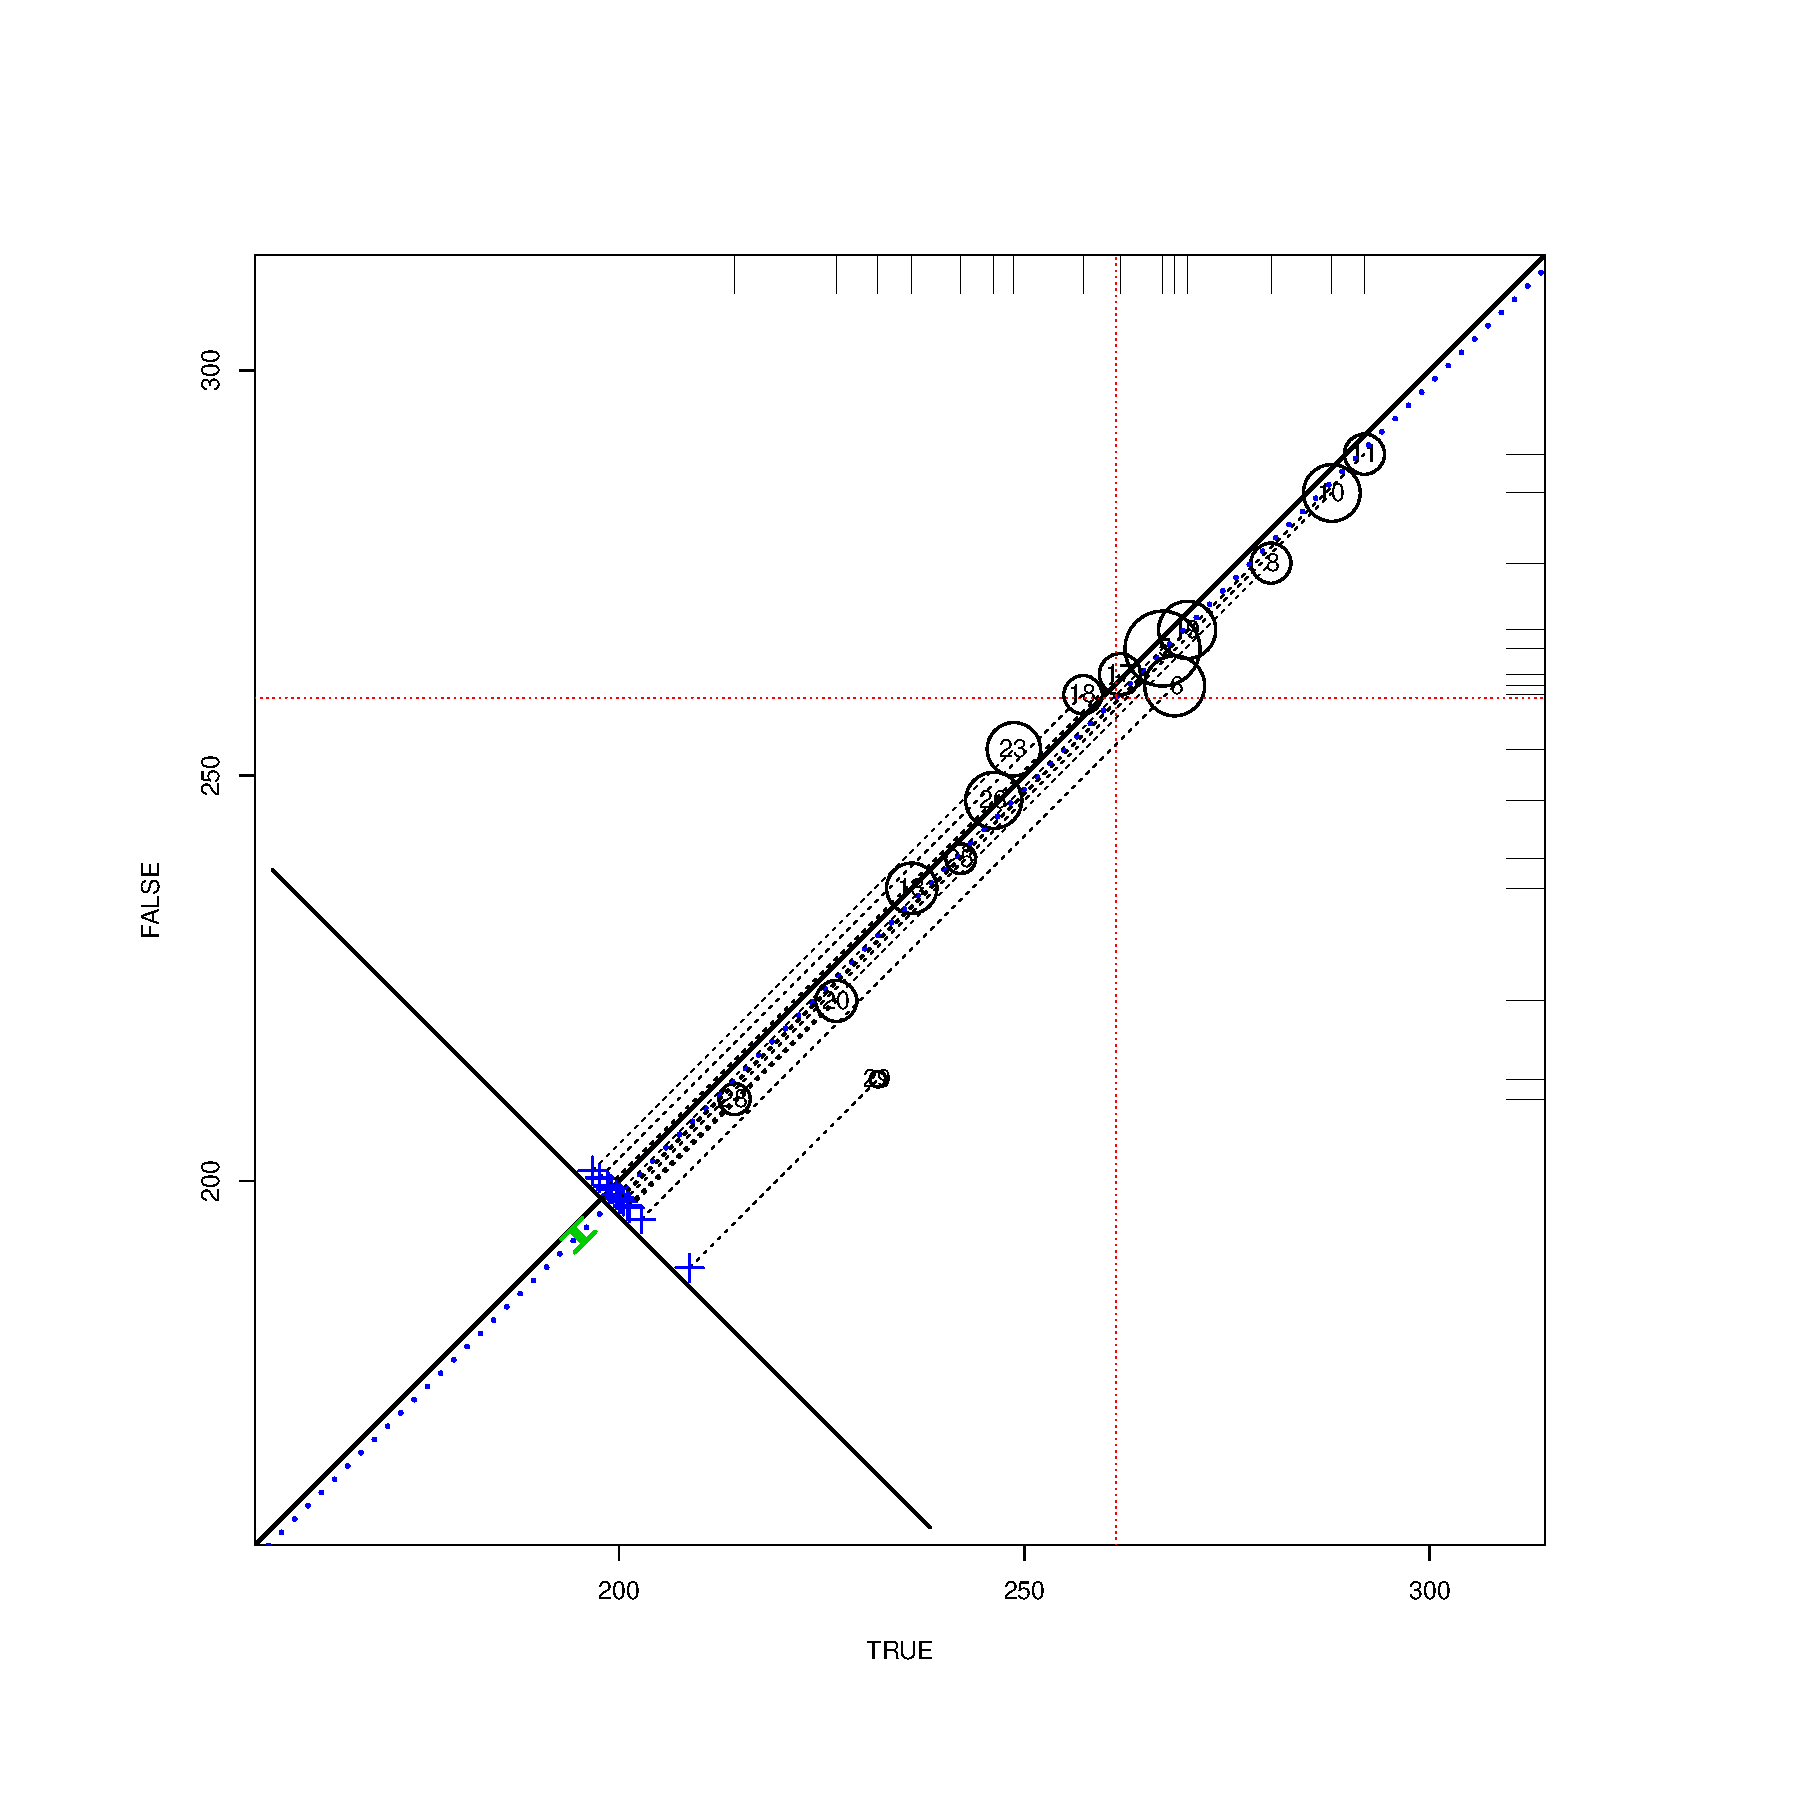
\includegraphics[height=.4\textheight,width=.4\textheight]{../Figures2009/g8read-circpsa-tree.pdf}
\caption{Propensity score assessment plot for classification tree stratification: Grade 8 reading}
\end{center}
\end{figure}

% latex table generated in R 3.0.2 by xtable 1.7-1 package
% Sun Feb 23 12:20:17 2014
\begin{table}[h!]
\centering
\caption{Classification trees stratification results for grade 8 reading} 
\label{g8read-circpsa-tree}
\begin{tabular}{lrr@{\extracolsep{.2cm}}rr}
  \hline
   & \multicolumn{2}{c}{Public} & \multicolumn{2}{c}{Charter} \\ \cline{2-3} \cline{4-5} Strata & Mean & n & Mean & n \\ \hline
5 & 265.67 & 14613 & 267.03 & 381 \\ 
  6 & 261.08 & 8482 & 268.53 & 163 \\ 
  8 & 276.22 & 3089 & 280.42 &  79 \\ 
  10 & 284.87 & 7238 & 287.92 & 265 \\ 
  11 & 289.66 & 3063 & 291.96 & 157 \\ 
  13 & 236.11 & 5341 & 236.11 & 233 \\ 
  17 & 262.51 & 3239 & 261.80 & 188 \\ 
  18 & 259.98 & 2725 & 257.24 & 112 \\ 
  19 & 267.97 & 7196 & 270.08 & 453 \\ 
  20 & 222.21 & 3127 & 226.81 & 250 \\ 
  23 & 253.26 & 5887 & 248.70 & 529 \\ 
  25 & 239.75 & 1400 & 242.16 & 119 \\ 
  26 & 246.96 & 6535 & 246.22 & 766 \\ 
  28 & 210.10 & 1606 & 214.26 &  84 \\ 
  29 & 212.56 & 269 & 231.94 &  33 \\ 
   \hline
\end{tabular}
\end{table}




%==================== Appendix G ====================================================================
\clearpage
\addcontentsline{toc}{subsection}{Appendix G: Multilevel PSA Covariate Balance Plots}
\section*{Appendix G\\Multilevel PSA Covariate Balance Plots}
\label{appendixG}

% Grade 4 math
\begin{figure}[h!]
\begin{center}
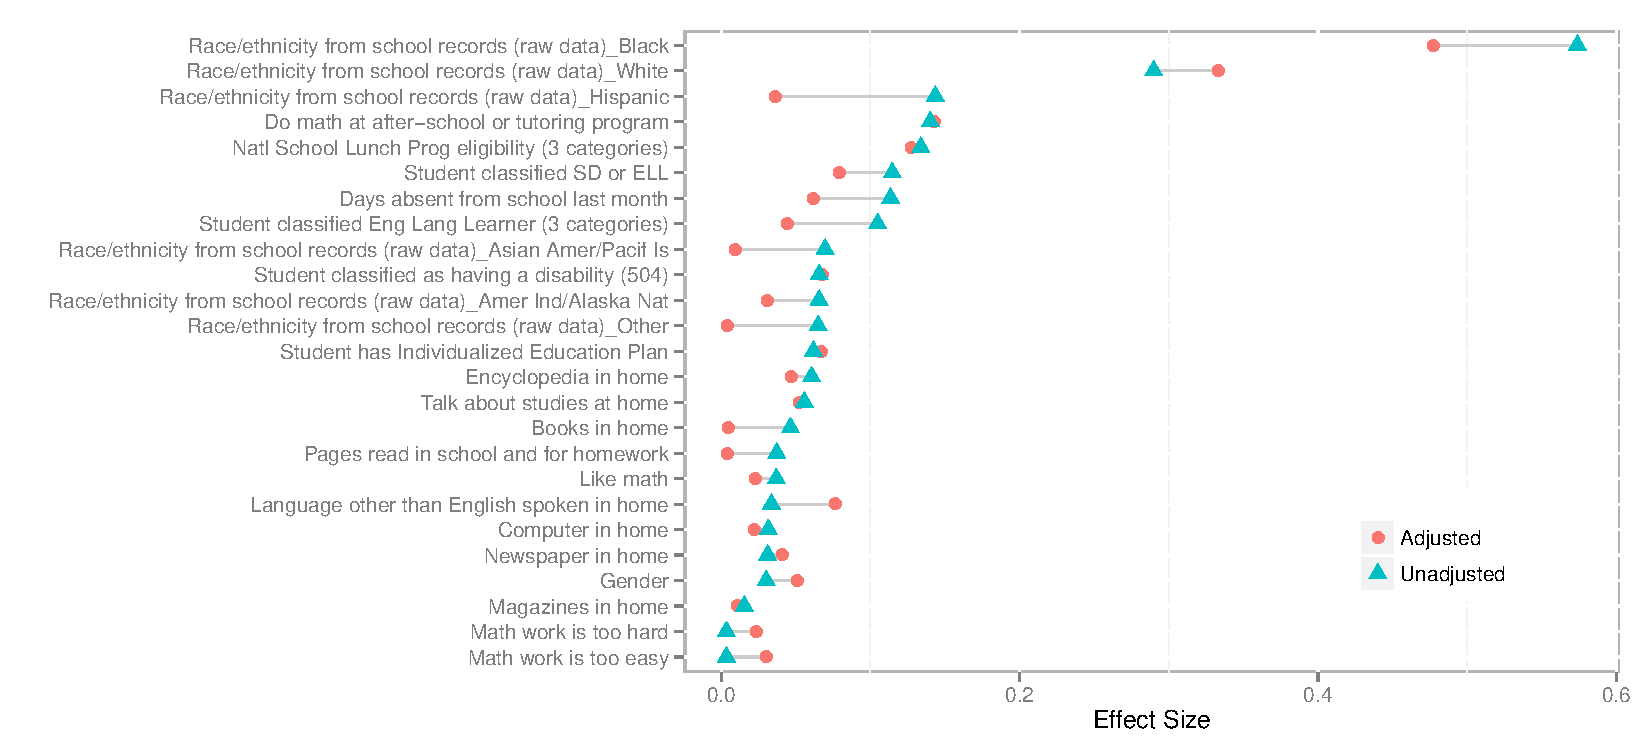
\includegraphics[width=\textwidth]{../Figures2009/g4math-mlpsa-lr-balance.pdf}
\caption{Multilevel PSA covariate balance plot logistic regression: Grade 4 math}
\end{center}
\end{figure}

\begin{figure}[h!]
\begin{center}
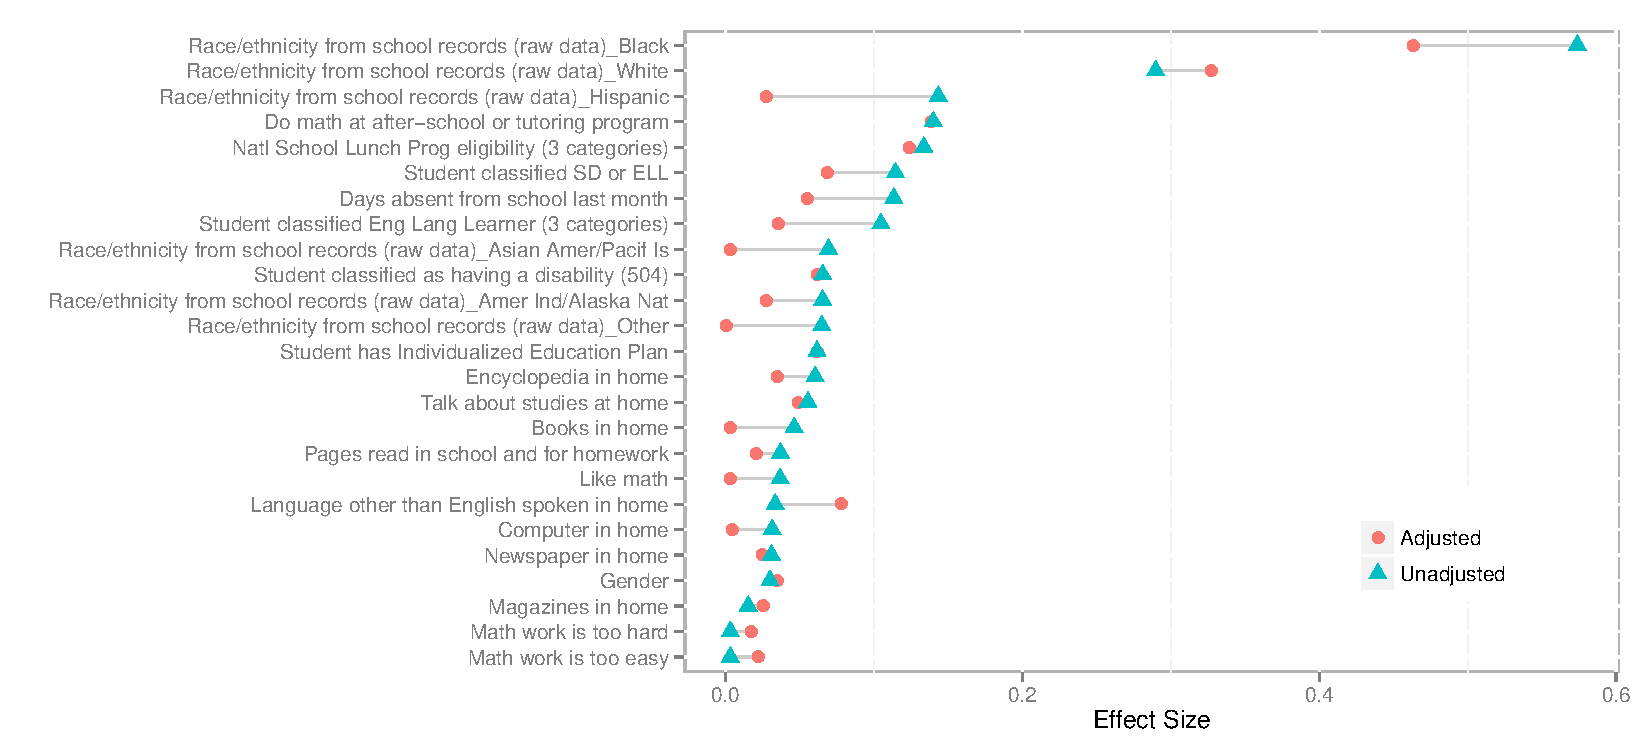
\includegraphics[width=\textwidth]{../Figures2009/g4math-mlpsa-lrAIC-balance.pdf}
\caption{Multilevel PSA covariate balance plot logistic regression AIC: Grade 4 math}
\end{center}
\end{figure}

\begin{figure}[h!]
\begin{center}
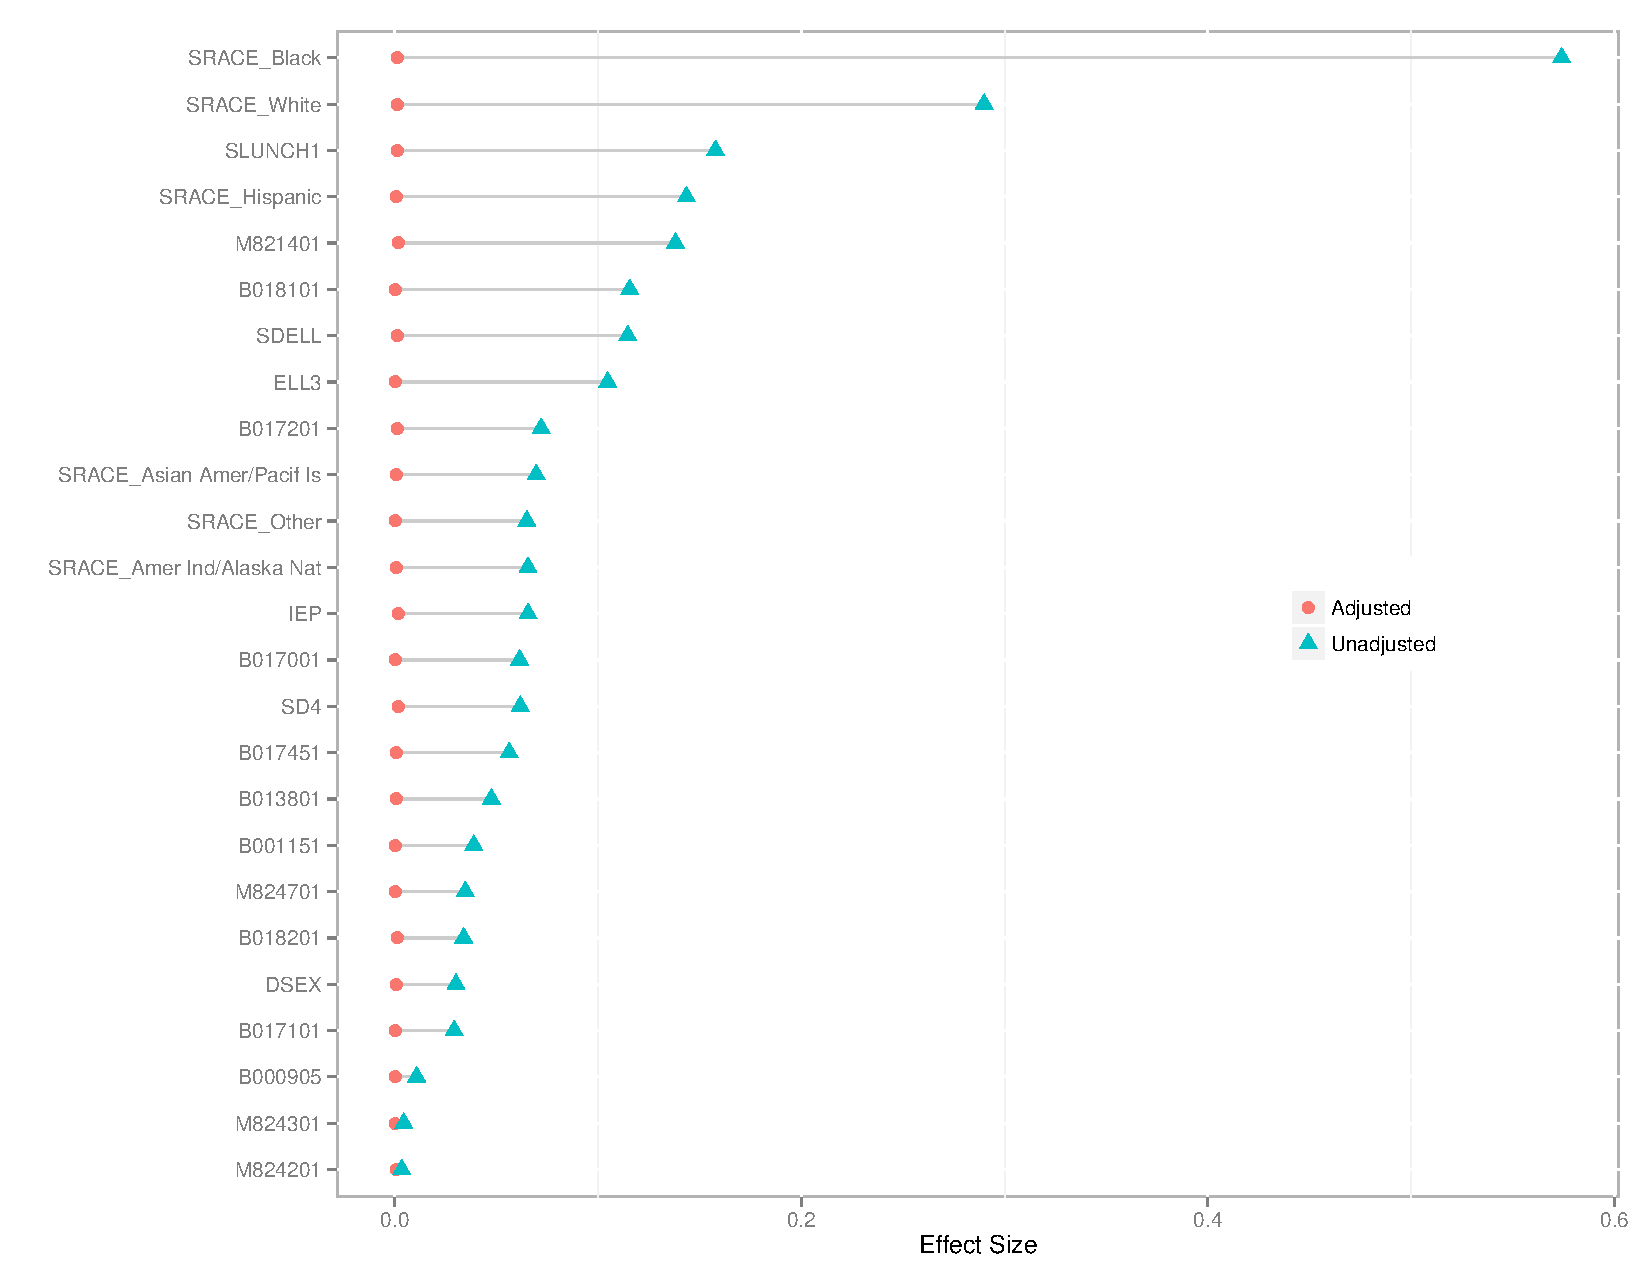
\includegraphics[width=\textwidth]{../Figures2009/g4math-mlpsa-ctree-balance.pdf}
\caption{Multilevel PSA covariate balance plot classification tree: Grade 4 math}
\end{center}
\end{figure}

% Grade 4 reading
\begin{figure}[h!]
\begin{center}
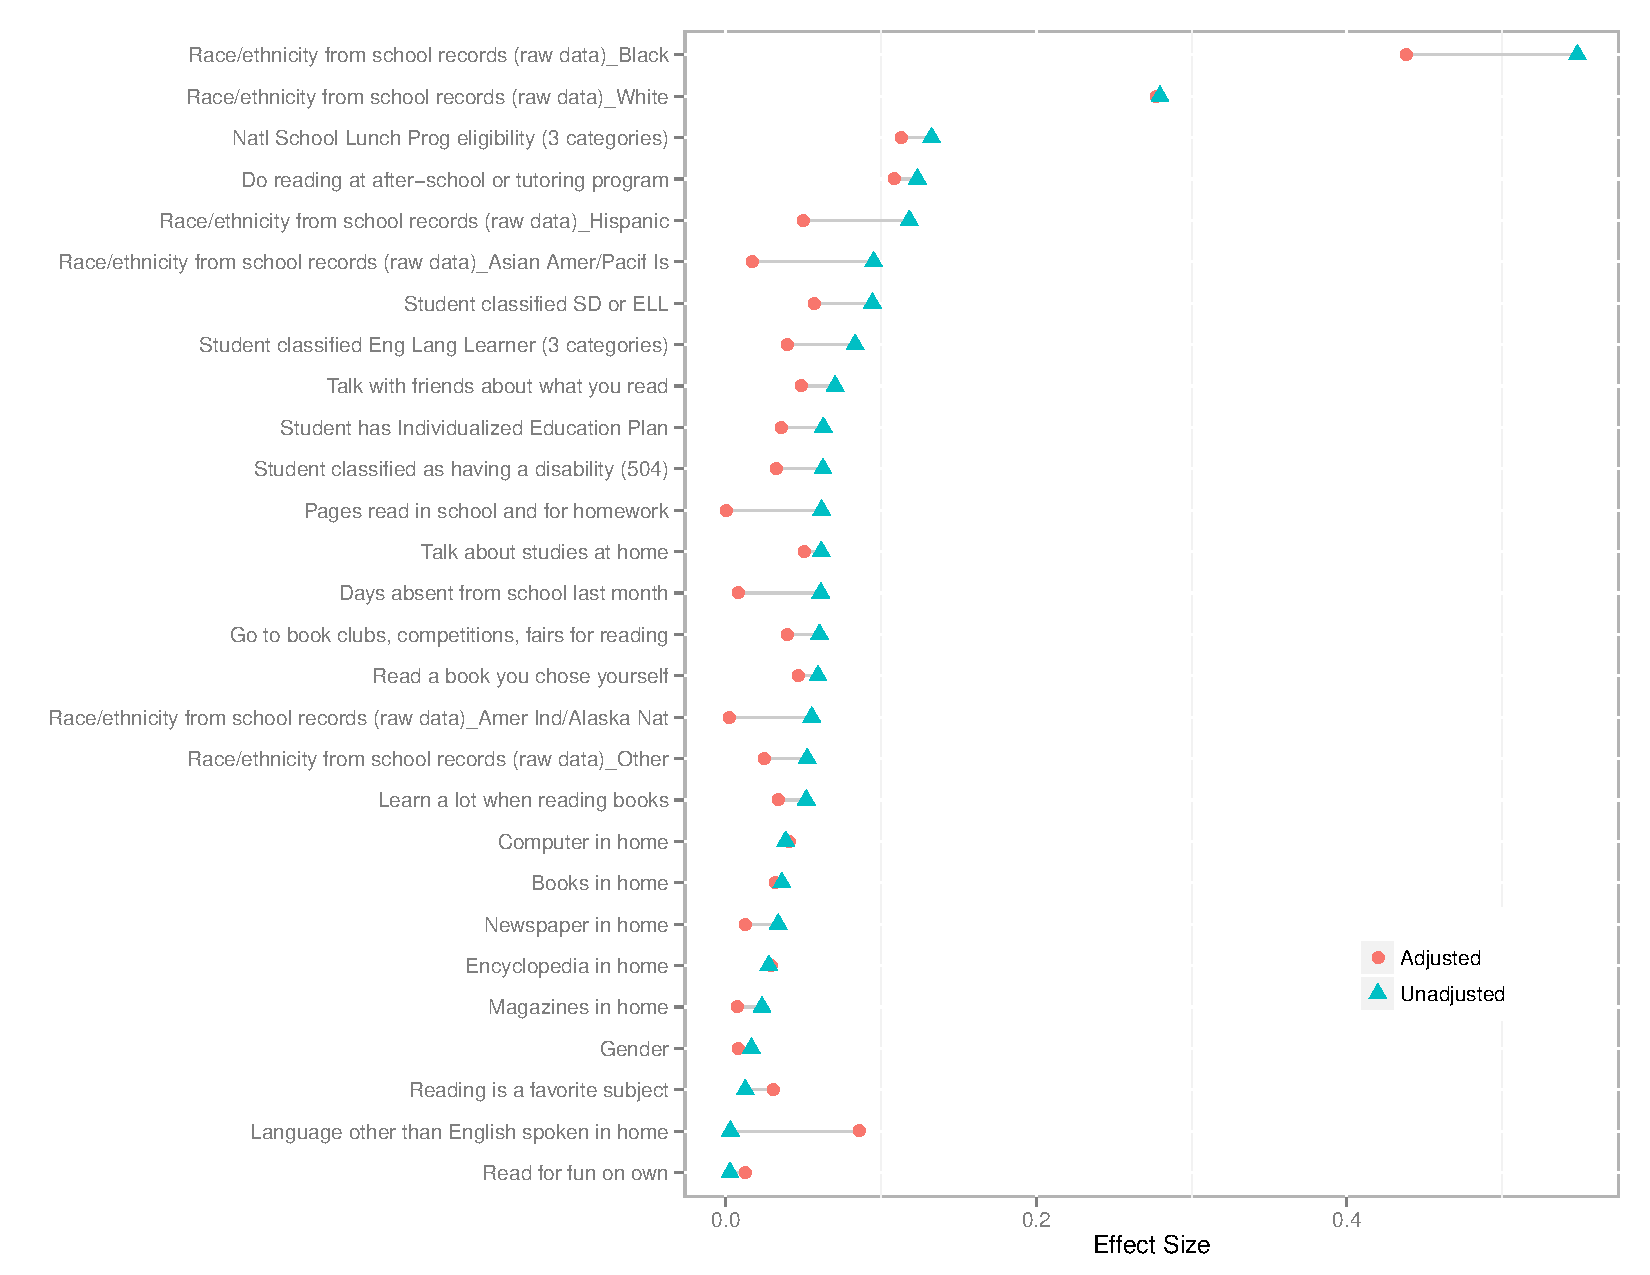
\includegraphics[width=\textwidth]{../Figures2009/g4read-mlpsa-lr-balance.pdf}
\caption{Multilevel PSA covariate balance plot logistic regression: Grade 4 reading}
\end{center}
\end{figure}

\begin{figure}[h!]
\begin{center}
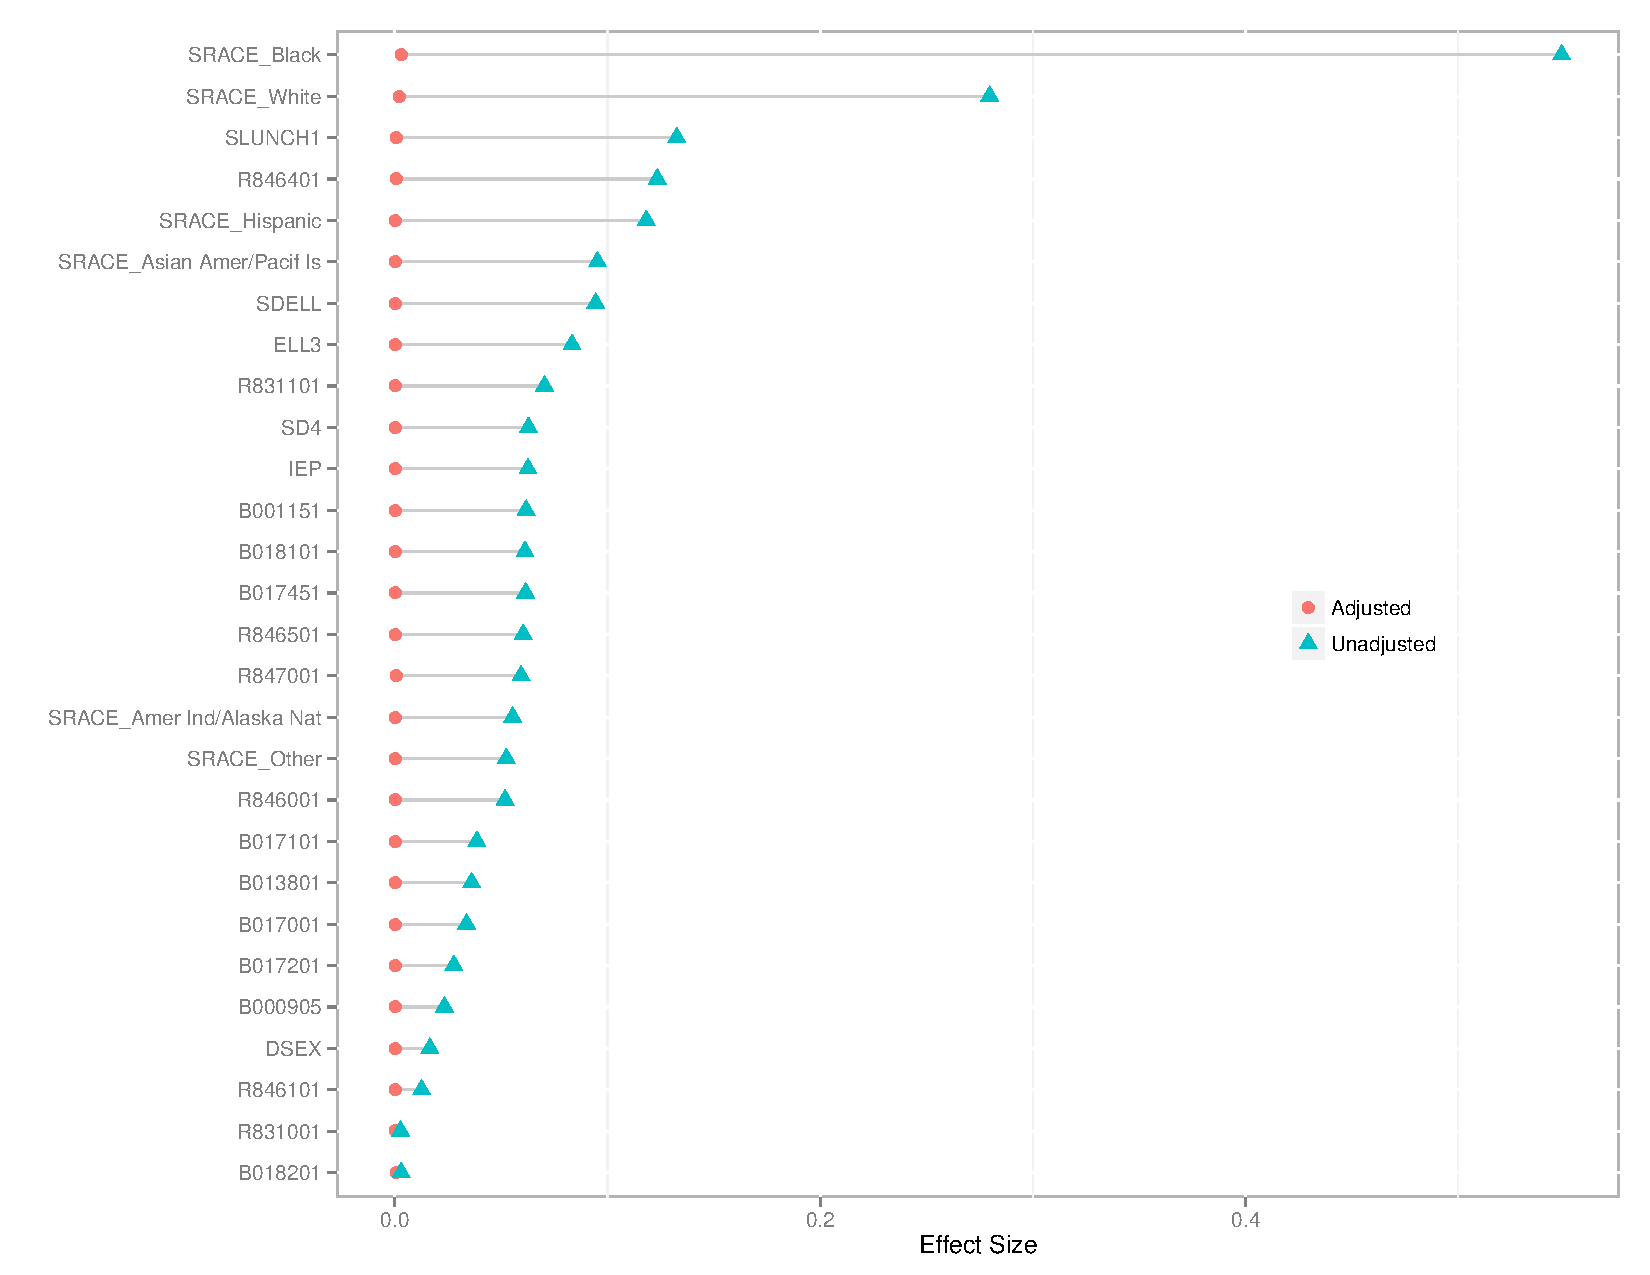
\includegraphics[width=\textwidth]{../Figures2009/g4read-mlpsa-lrAIC-balance.pdf}
\caption{Multilevel PSA covariate balance plot logistic regression AIC: Grade 4 reading}
\end{center}
\end{figure}

\begin{figure}[h!]
\begin{center}
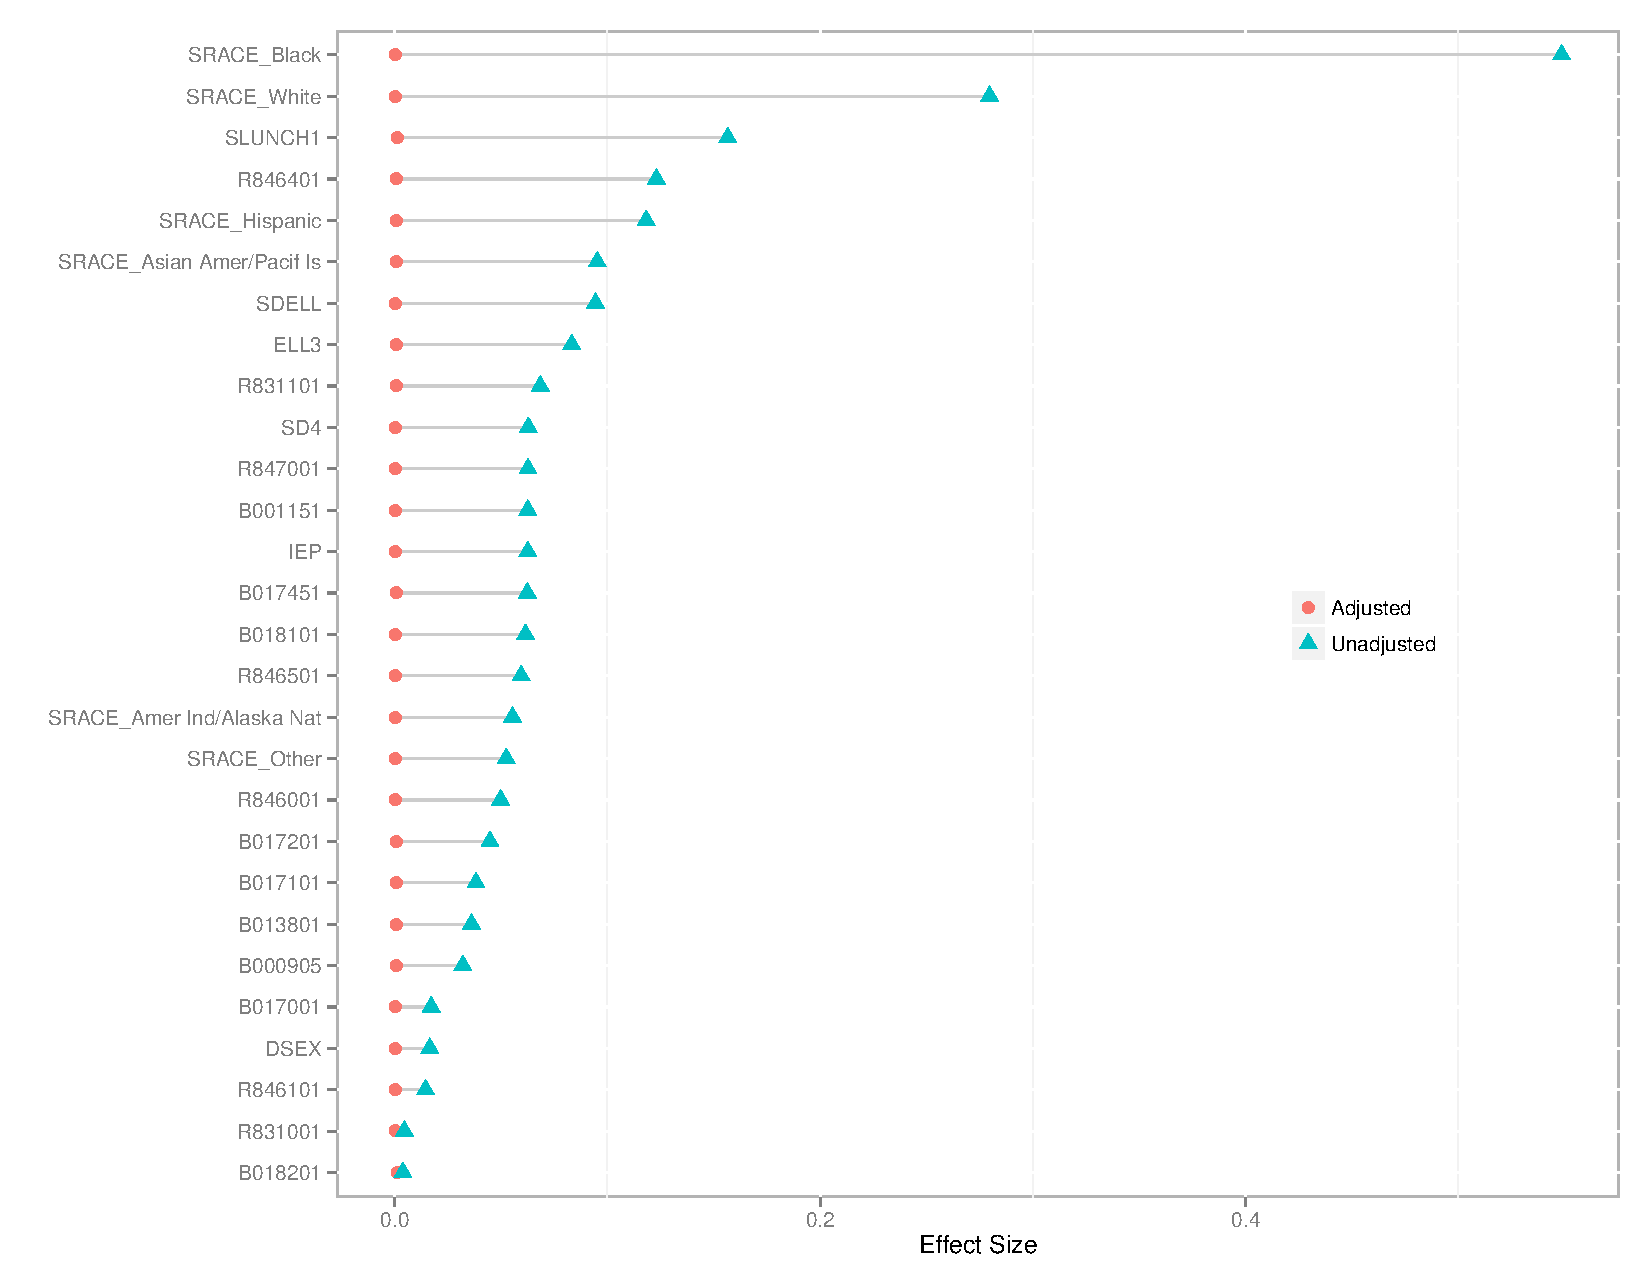
\includegraphics[width=\textwidth]{../Figures2009/g4read-mlpsa-ctree-balance.pdf}
\caption{Multilevel PSA covariate balance plot classification tree: Grade 4 reading}
\end{center}
\end{figure}

% Grade 8 math
\begin{figure}[h!]
\begin{center}
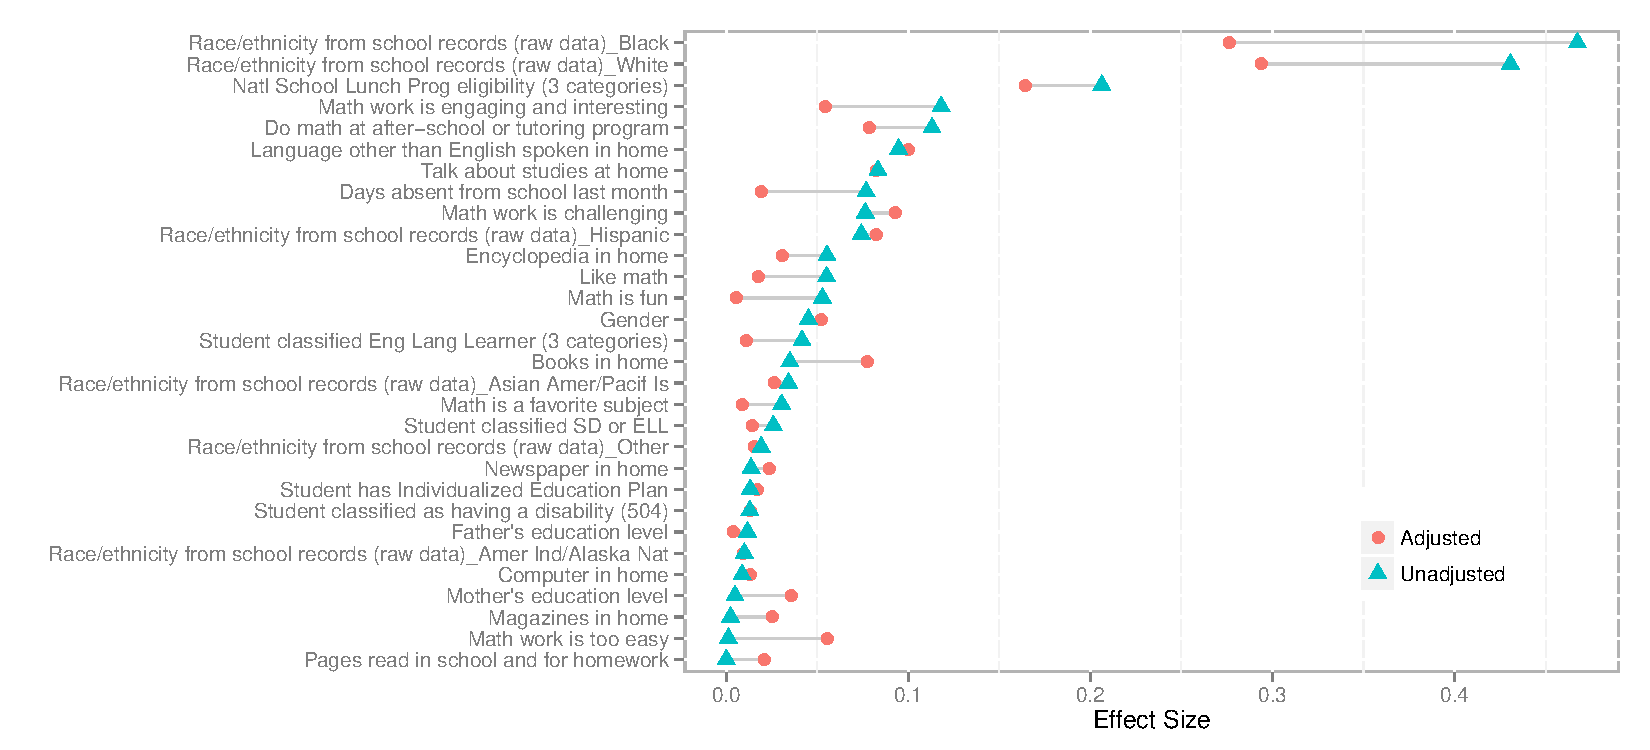
\includegraphics[width=\textwidth]{../Figures2009/g8math-mlpsa-lr-balance.pdf}
\caption{Multilevel PSA covariate balance plot logistic regression: Grade 8 math}
\end{center}
\end{figure}

\begin{figure}[h!]
\begin{center}
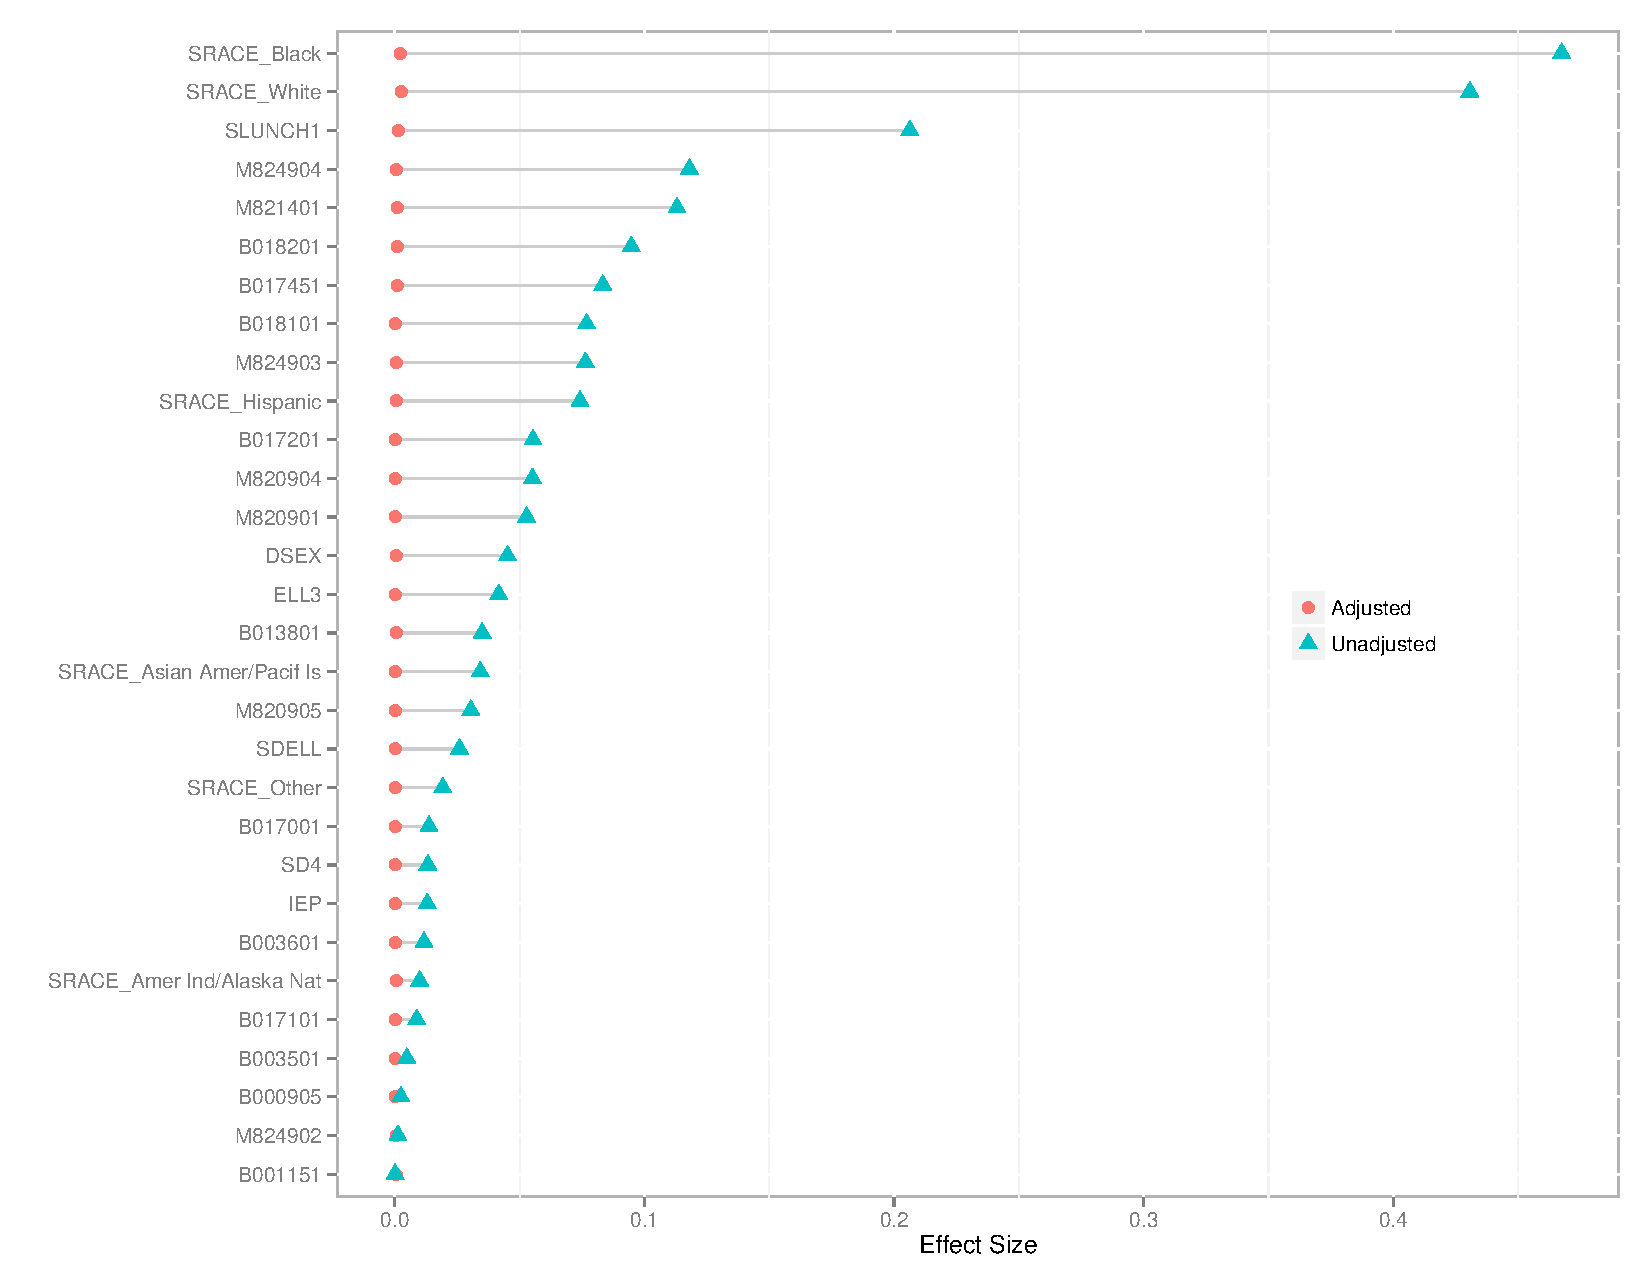
\includegraphics[width=\textwidth]{../Figures2009/g8math-mlpsa-lrAIC-balance.pdf}
\caption{Multilevel PSA covariate balance plot logistic regression AIC: Grade 8 math}
\end{center}
\end{figure}

\begin{figure}[h!]
\begin{center}
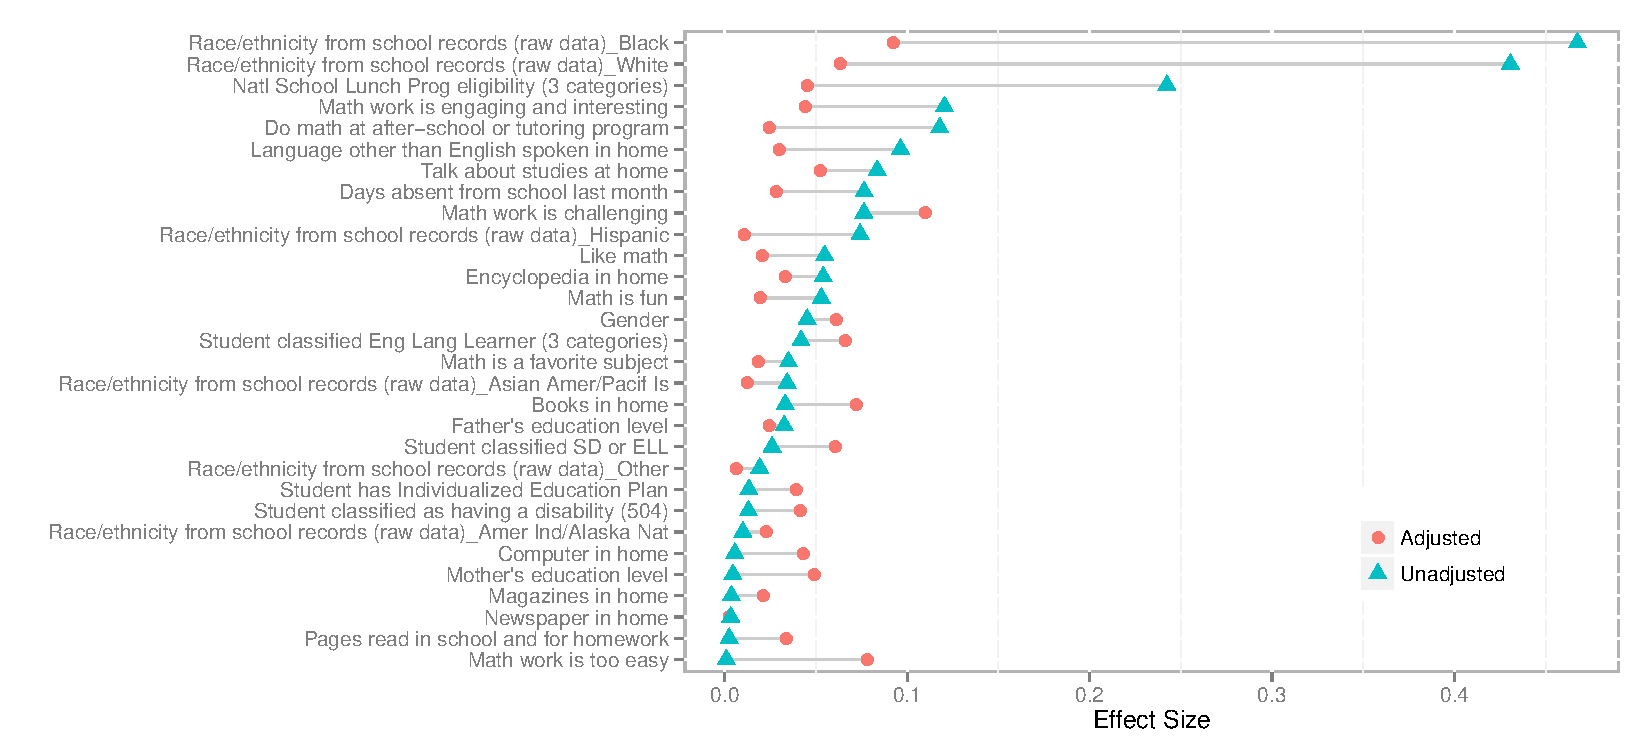
\includegraphics[width=\textwidth]{../Figures2009/g8math-mlpsa-ctree-balance.pdf}
\caption{Multilevel PSA covariate balance plot classification tree: Grade 8 math}
\end{center}
\end{figure}

% Grade 8 reading
\begin{figure}[h!]
\begin{center}
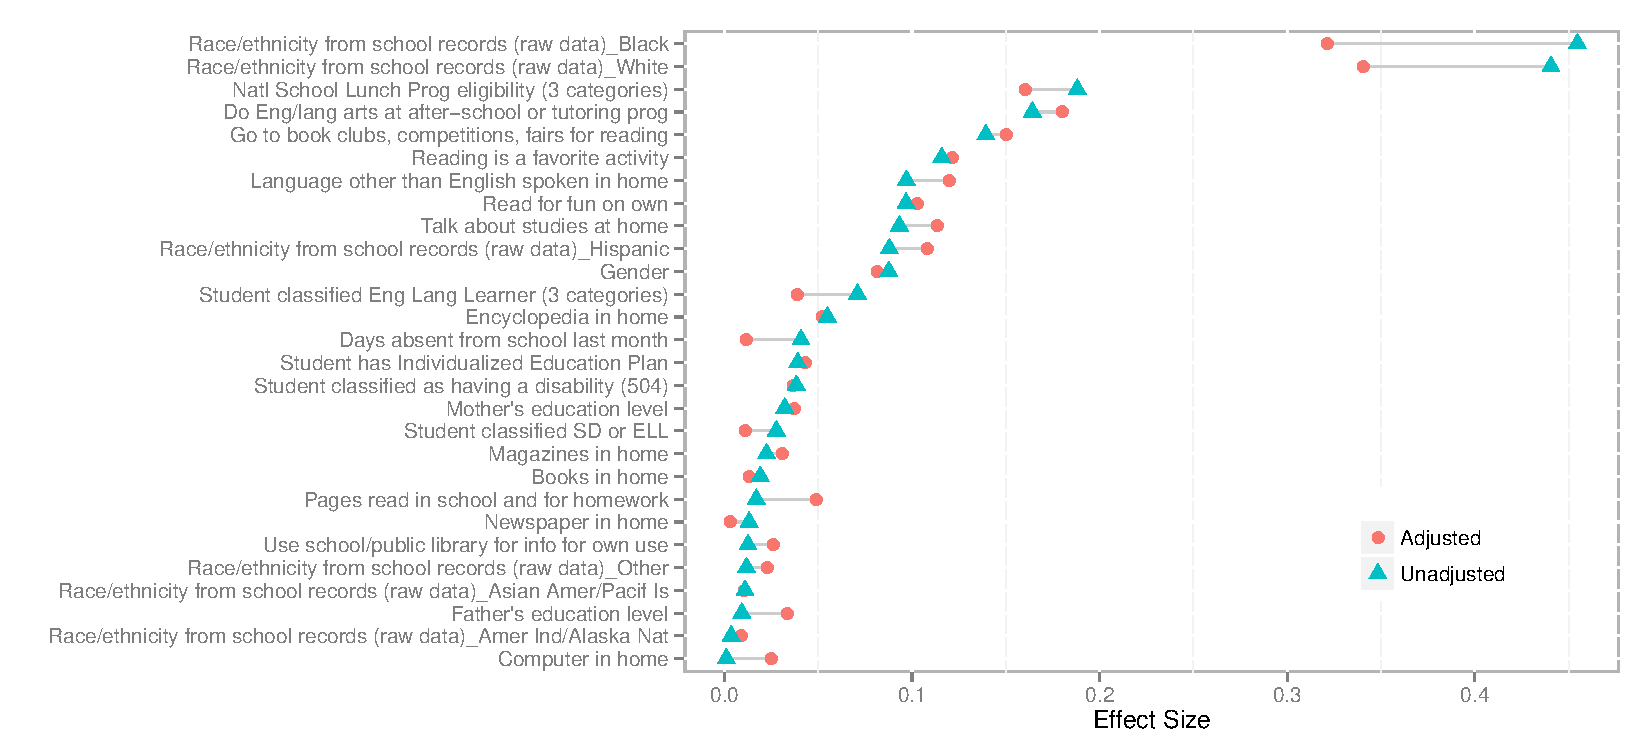
\includegraphics[width=\textwidth]{../Figures2009/g8read-mlpsa-lr-balance.pdf}
\caption{Multilevel PSA covariate balance plot logistic regression: Grade 8 reading}
\end{center}
\end{figure}

\begin{figure}[h!]
\begin{center}
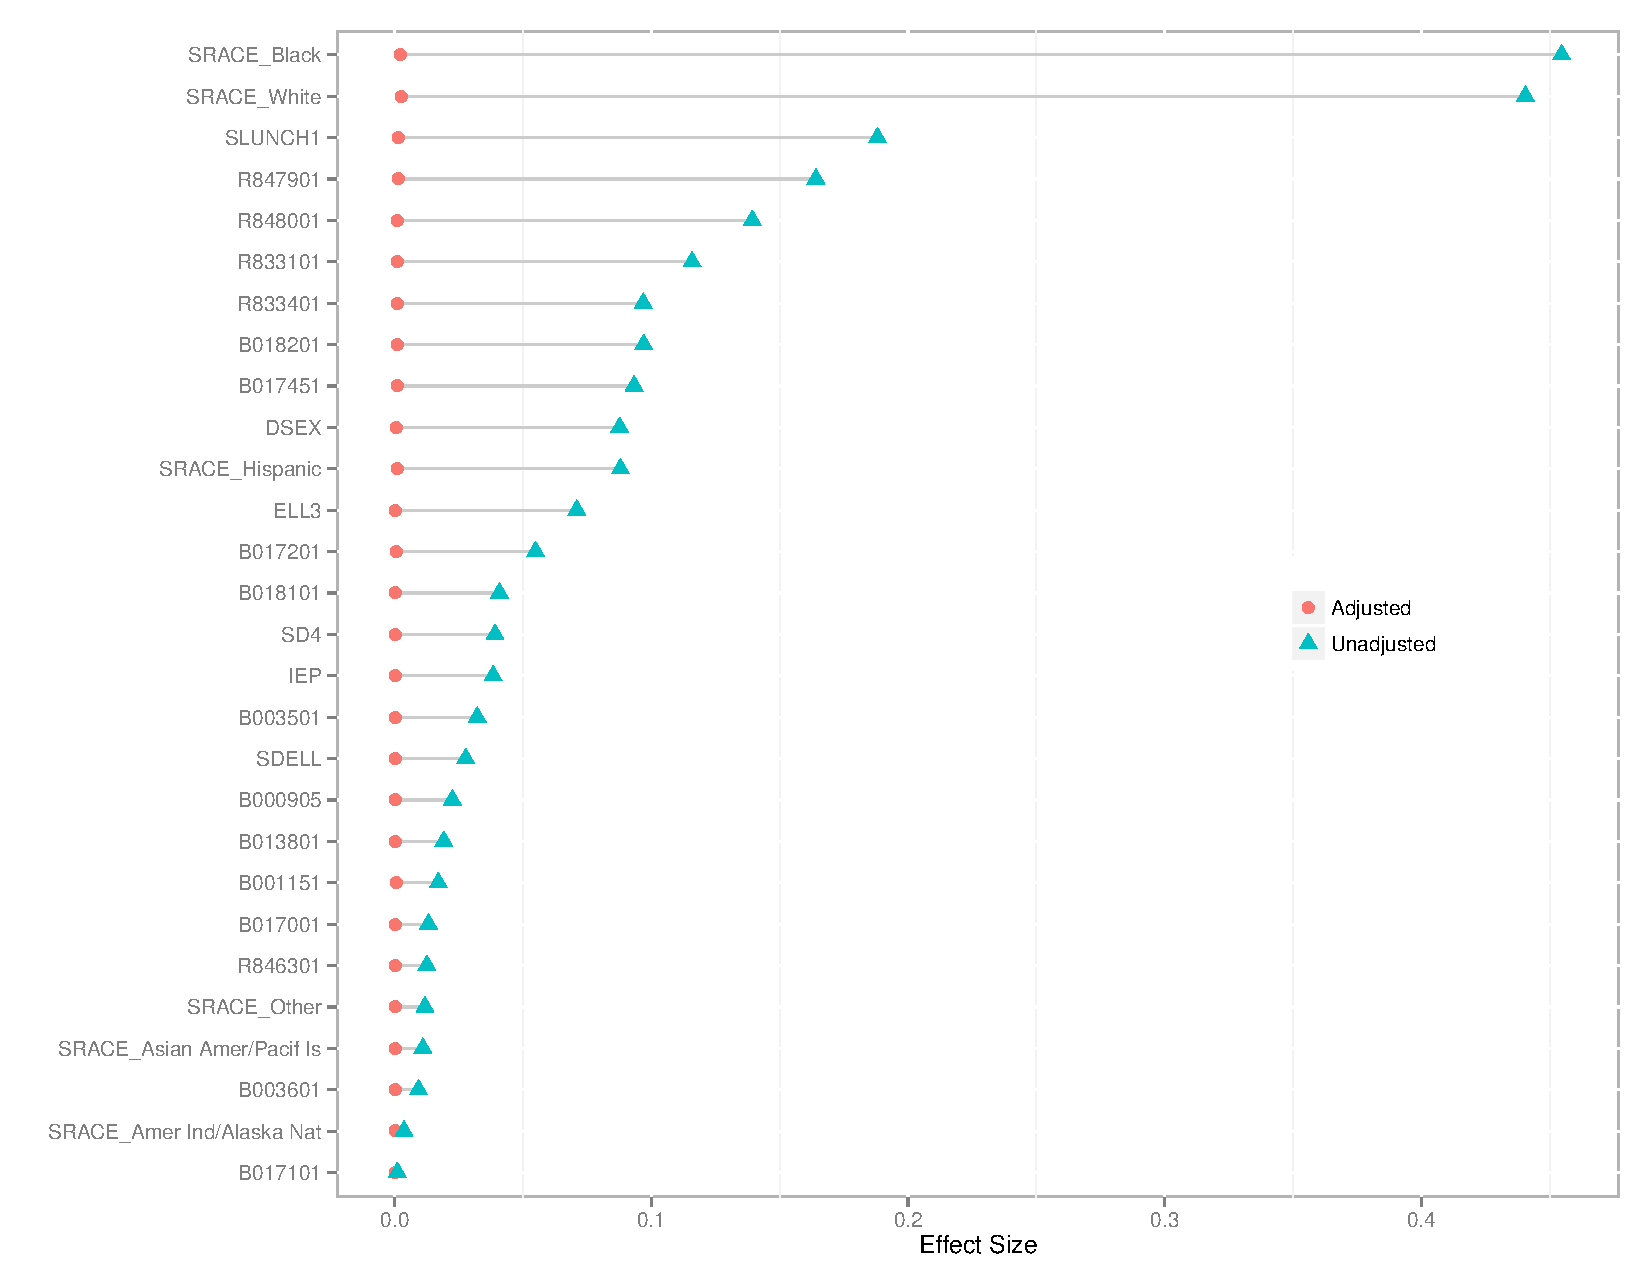
\includegraphics[width=\textwidth]{../Figures2009/g8read-mlpsa-lrAIC-balance.pdf}
\caption{Multilevel PSA covariate balance plot logistic regression AIC: Grade 8 reading}
\end{center}
\end{figure}

\begin{figure}[h!]
\begin{center}
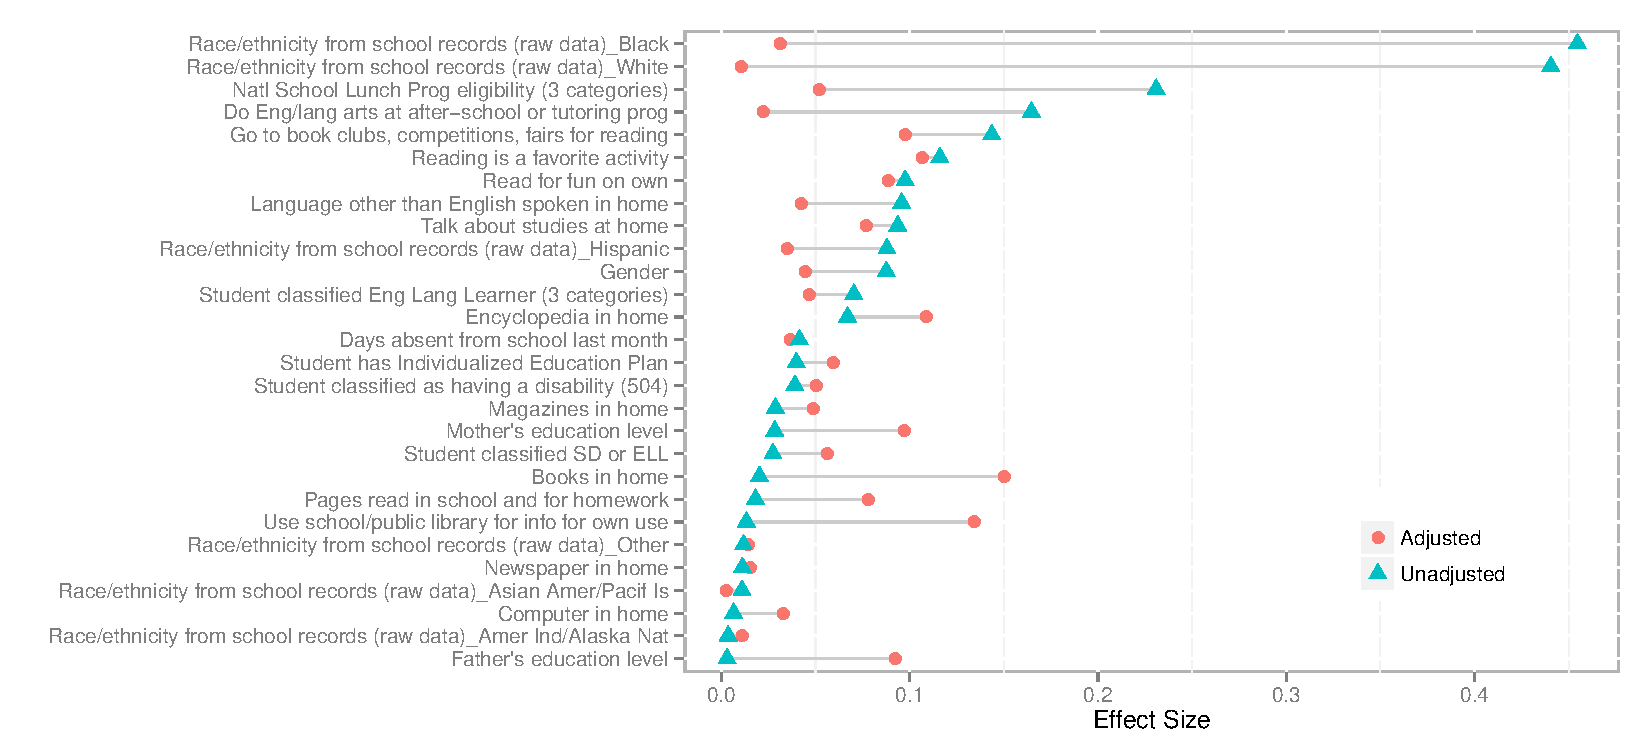
\includegraphics[width=\textwidth]{../Figures2009/g8read-mlpsa-ctree-balance.pdf}
\caption{Multilevel PSA covariate balance plot classification tree: Grade 8 reading}
\end{center}
\end{figure}


%==================== Appendix H ====================================================================
\clearpage
\addcontentsline{toc}{subsection}{Appendix H: Multilevel PSA Results}
\section*{Appendix H\\Multilevel PSA Results}
\label{appendixH}

% Grade 4 reading
\begin{figure}[h!]
\begin{center}
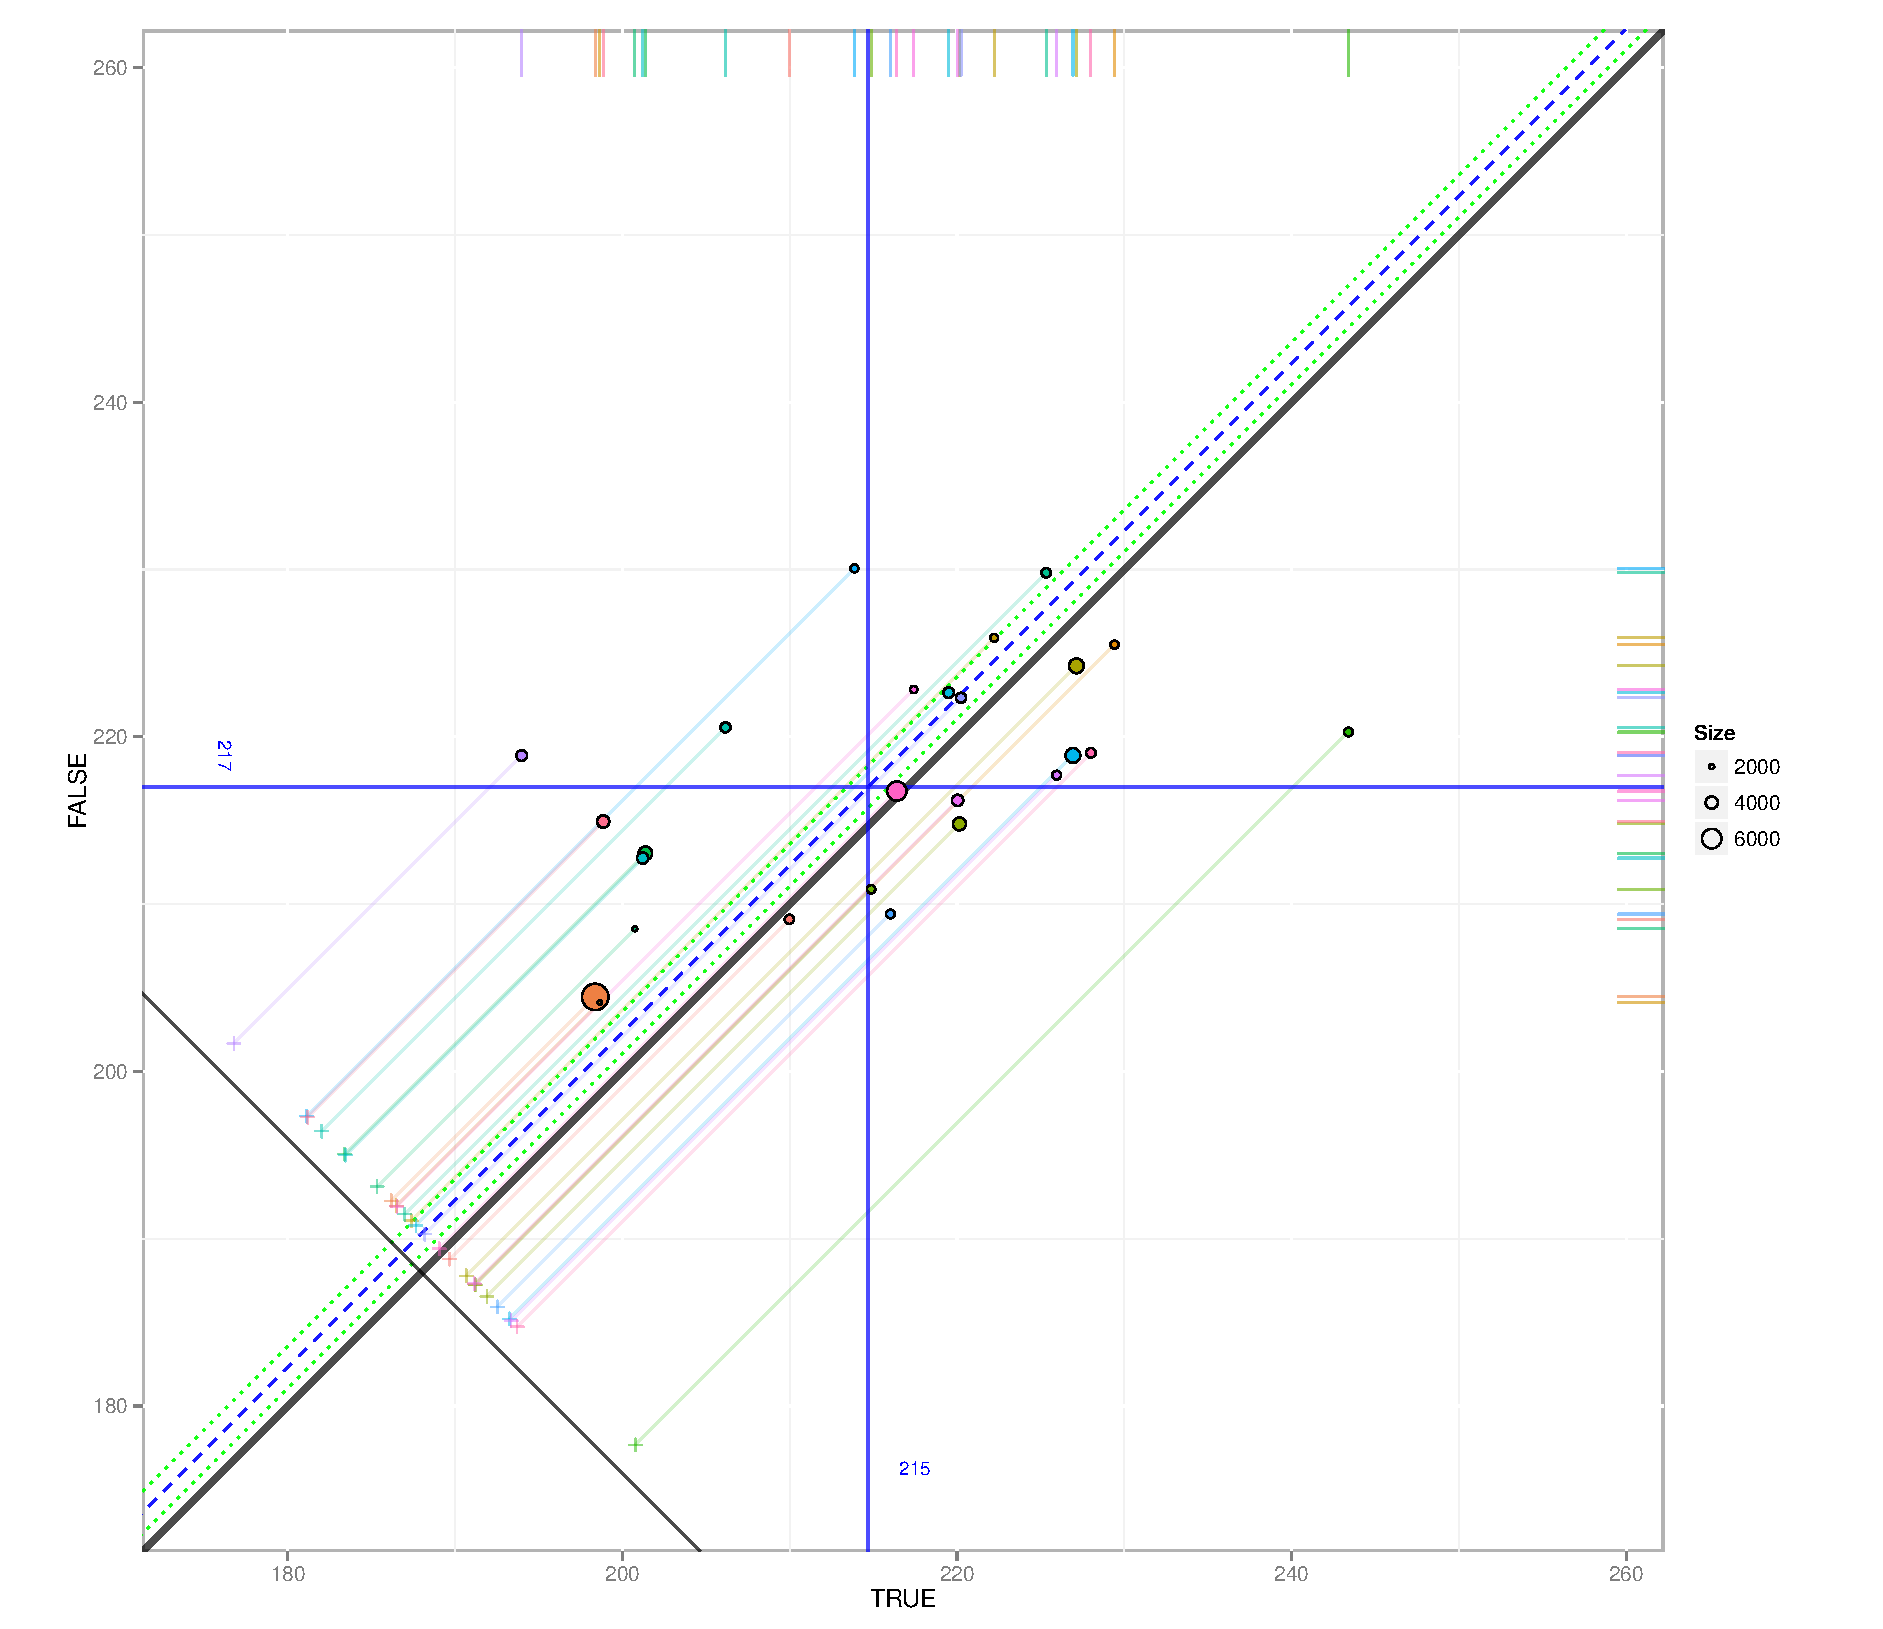
\includegraphics[width=\textwidth]{../Figures2009/g4read-mlpsa-lr-circ.pdf}
\caption{Multilevel PSA assessment plot logistic regression: Grade 4 reading}
\end{center}
\end{figure}

\begin{figure}[h!]
\begin{center}
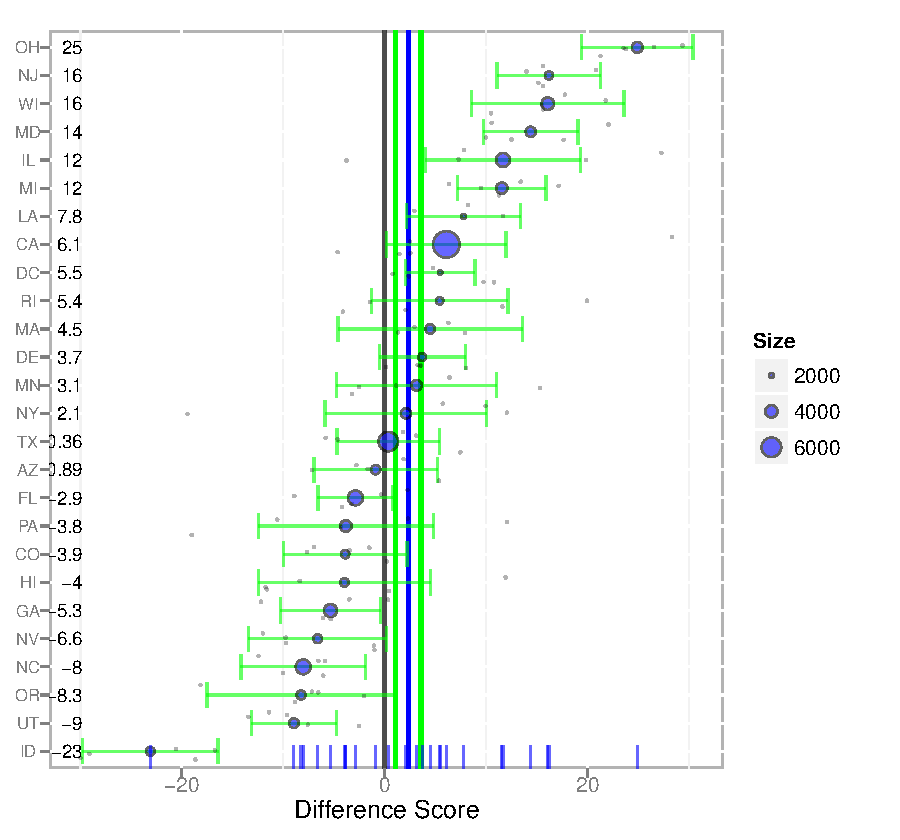
\includegraphics[width=\textwidth]{../Figures2009/g4read-mlpsa-lr-diff.pdf}
\caption{Multilevel PSA difference plot logistic regression: Grade 4 reading}
\end{center}
\end{figure}

\begin{figure}[h!]
\begin{center}
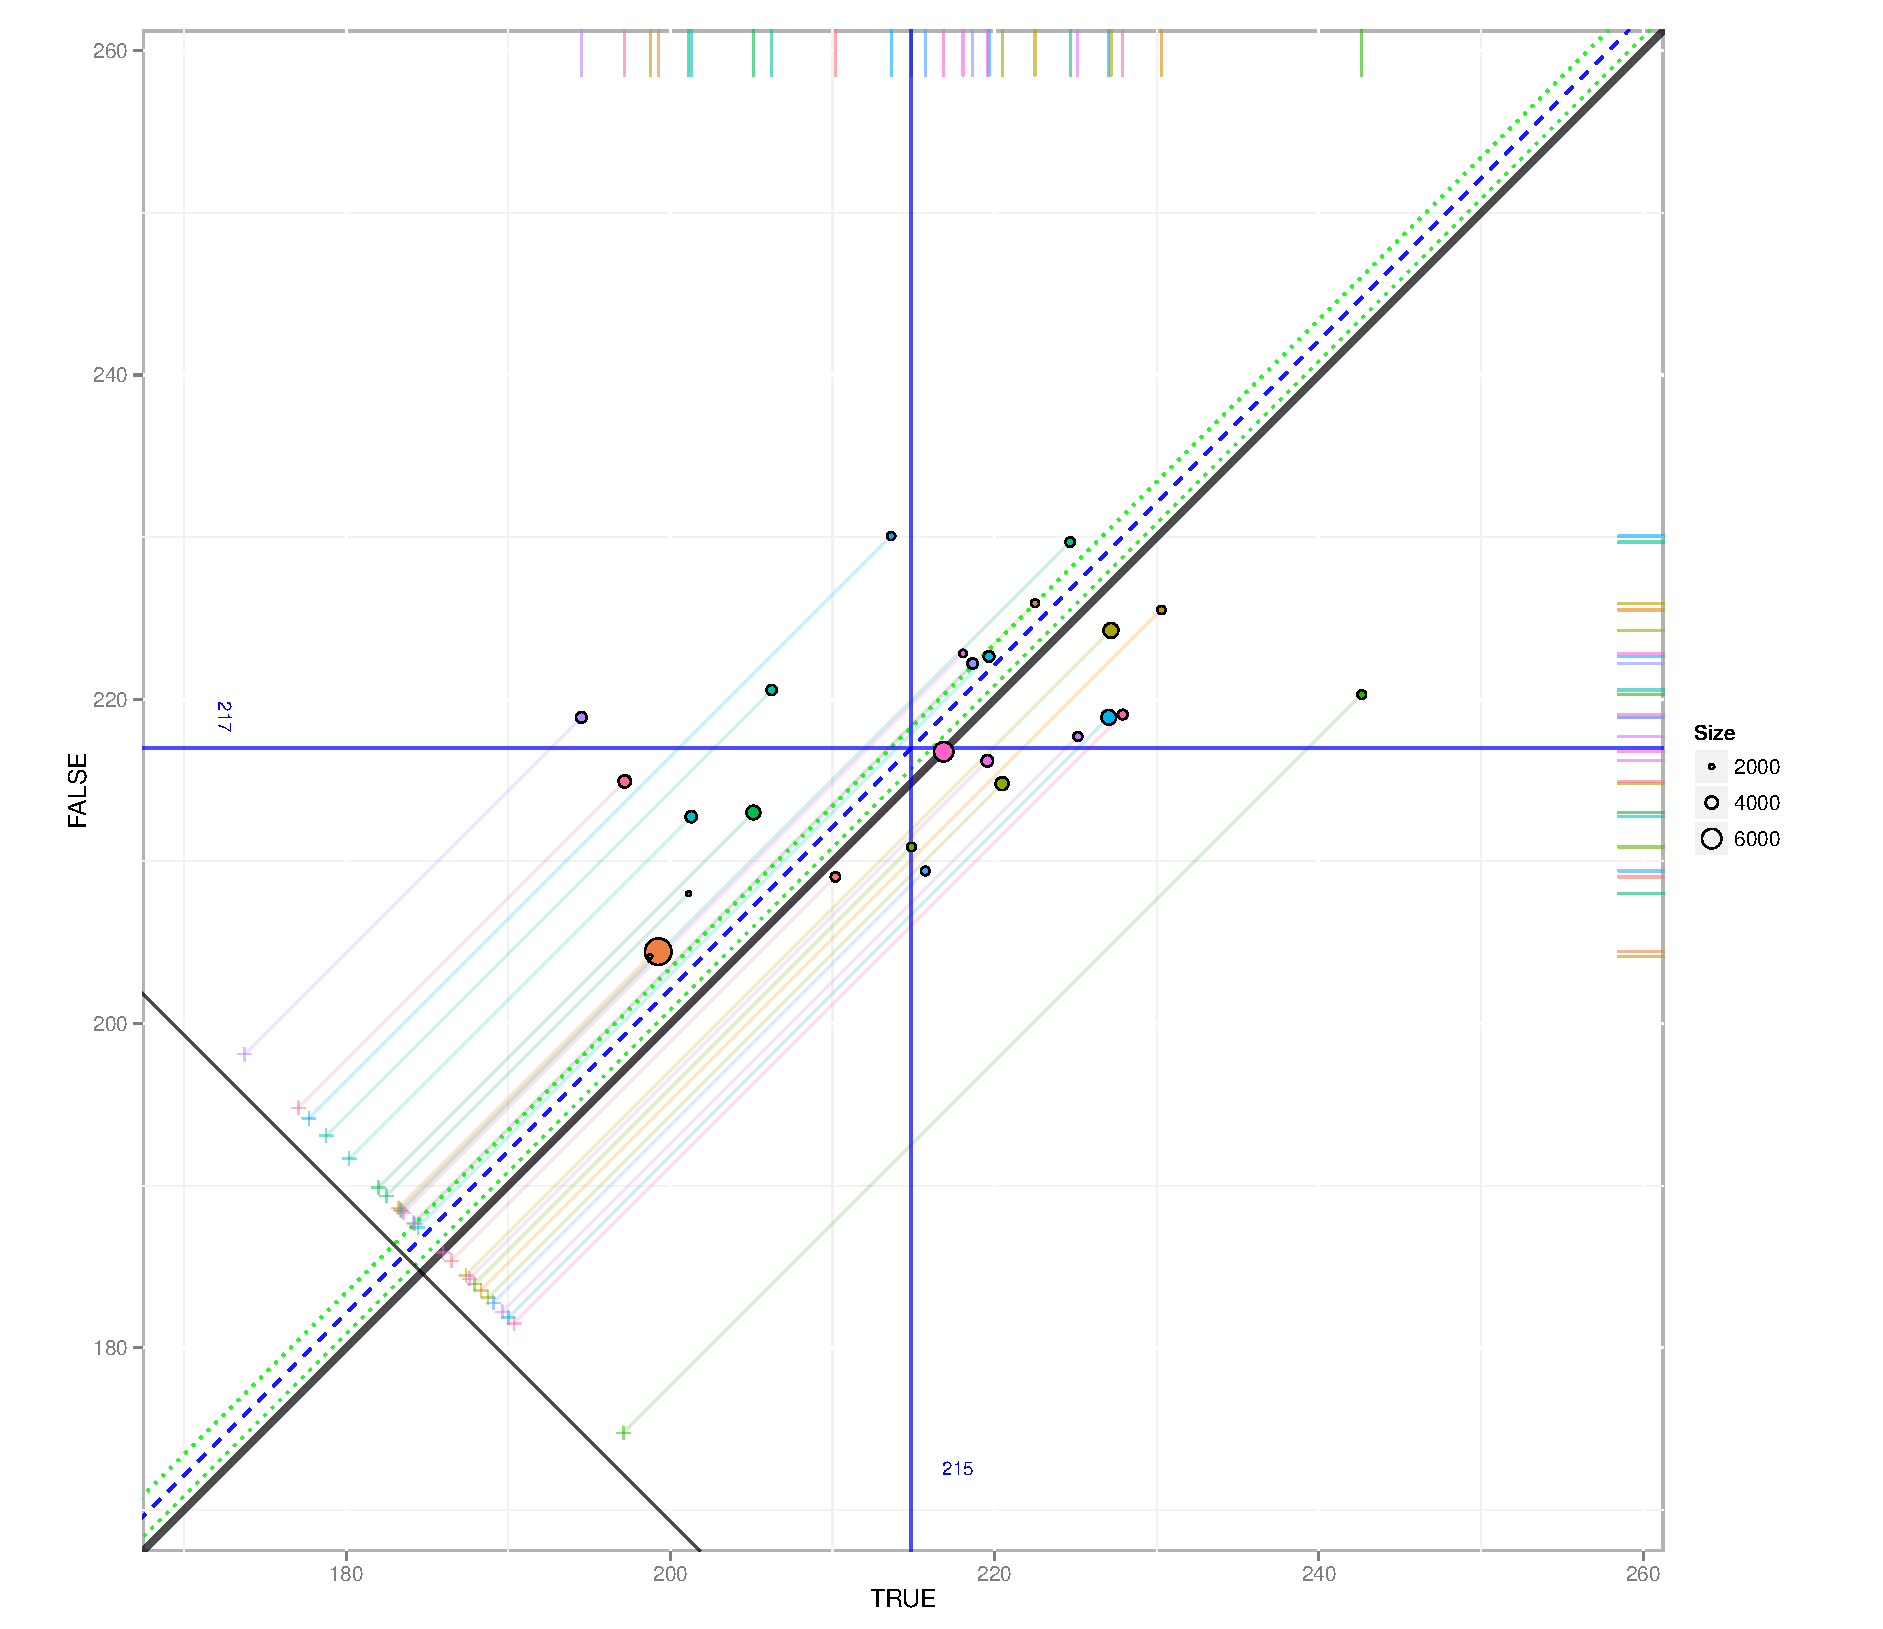
\includegraphics[width=\textwidth]{../Figures2009/g4read-mlpsa-lrAIC-circ.pdf}
\caption{Multilevel PSA assessment plot logistic regression AIC: Grade 4 reading}
\end{center}
\end{figure}

\begin{figure}[h!]
\begin{center}
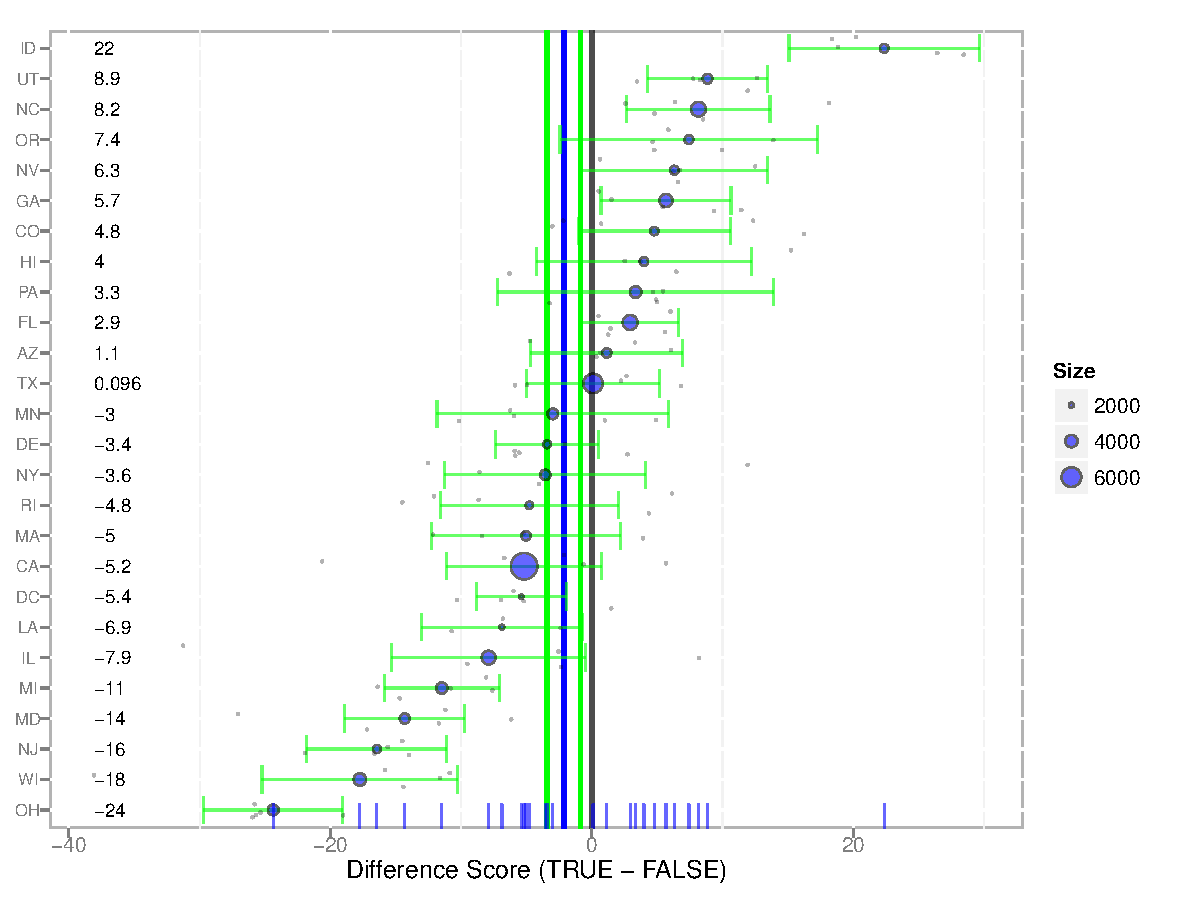
\includegraphics[width=\textwidth]{../Figures2009/g4read-mlpsa-lrAIC-diff.pdf}
\caption{Multilevel PSA difference plot logistic regression AIC: Grade 4 reading}
\end{center}
\end{figure}

\begin{figure}[h!]
\begin{center}
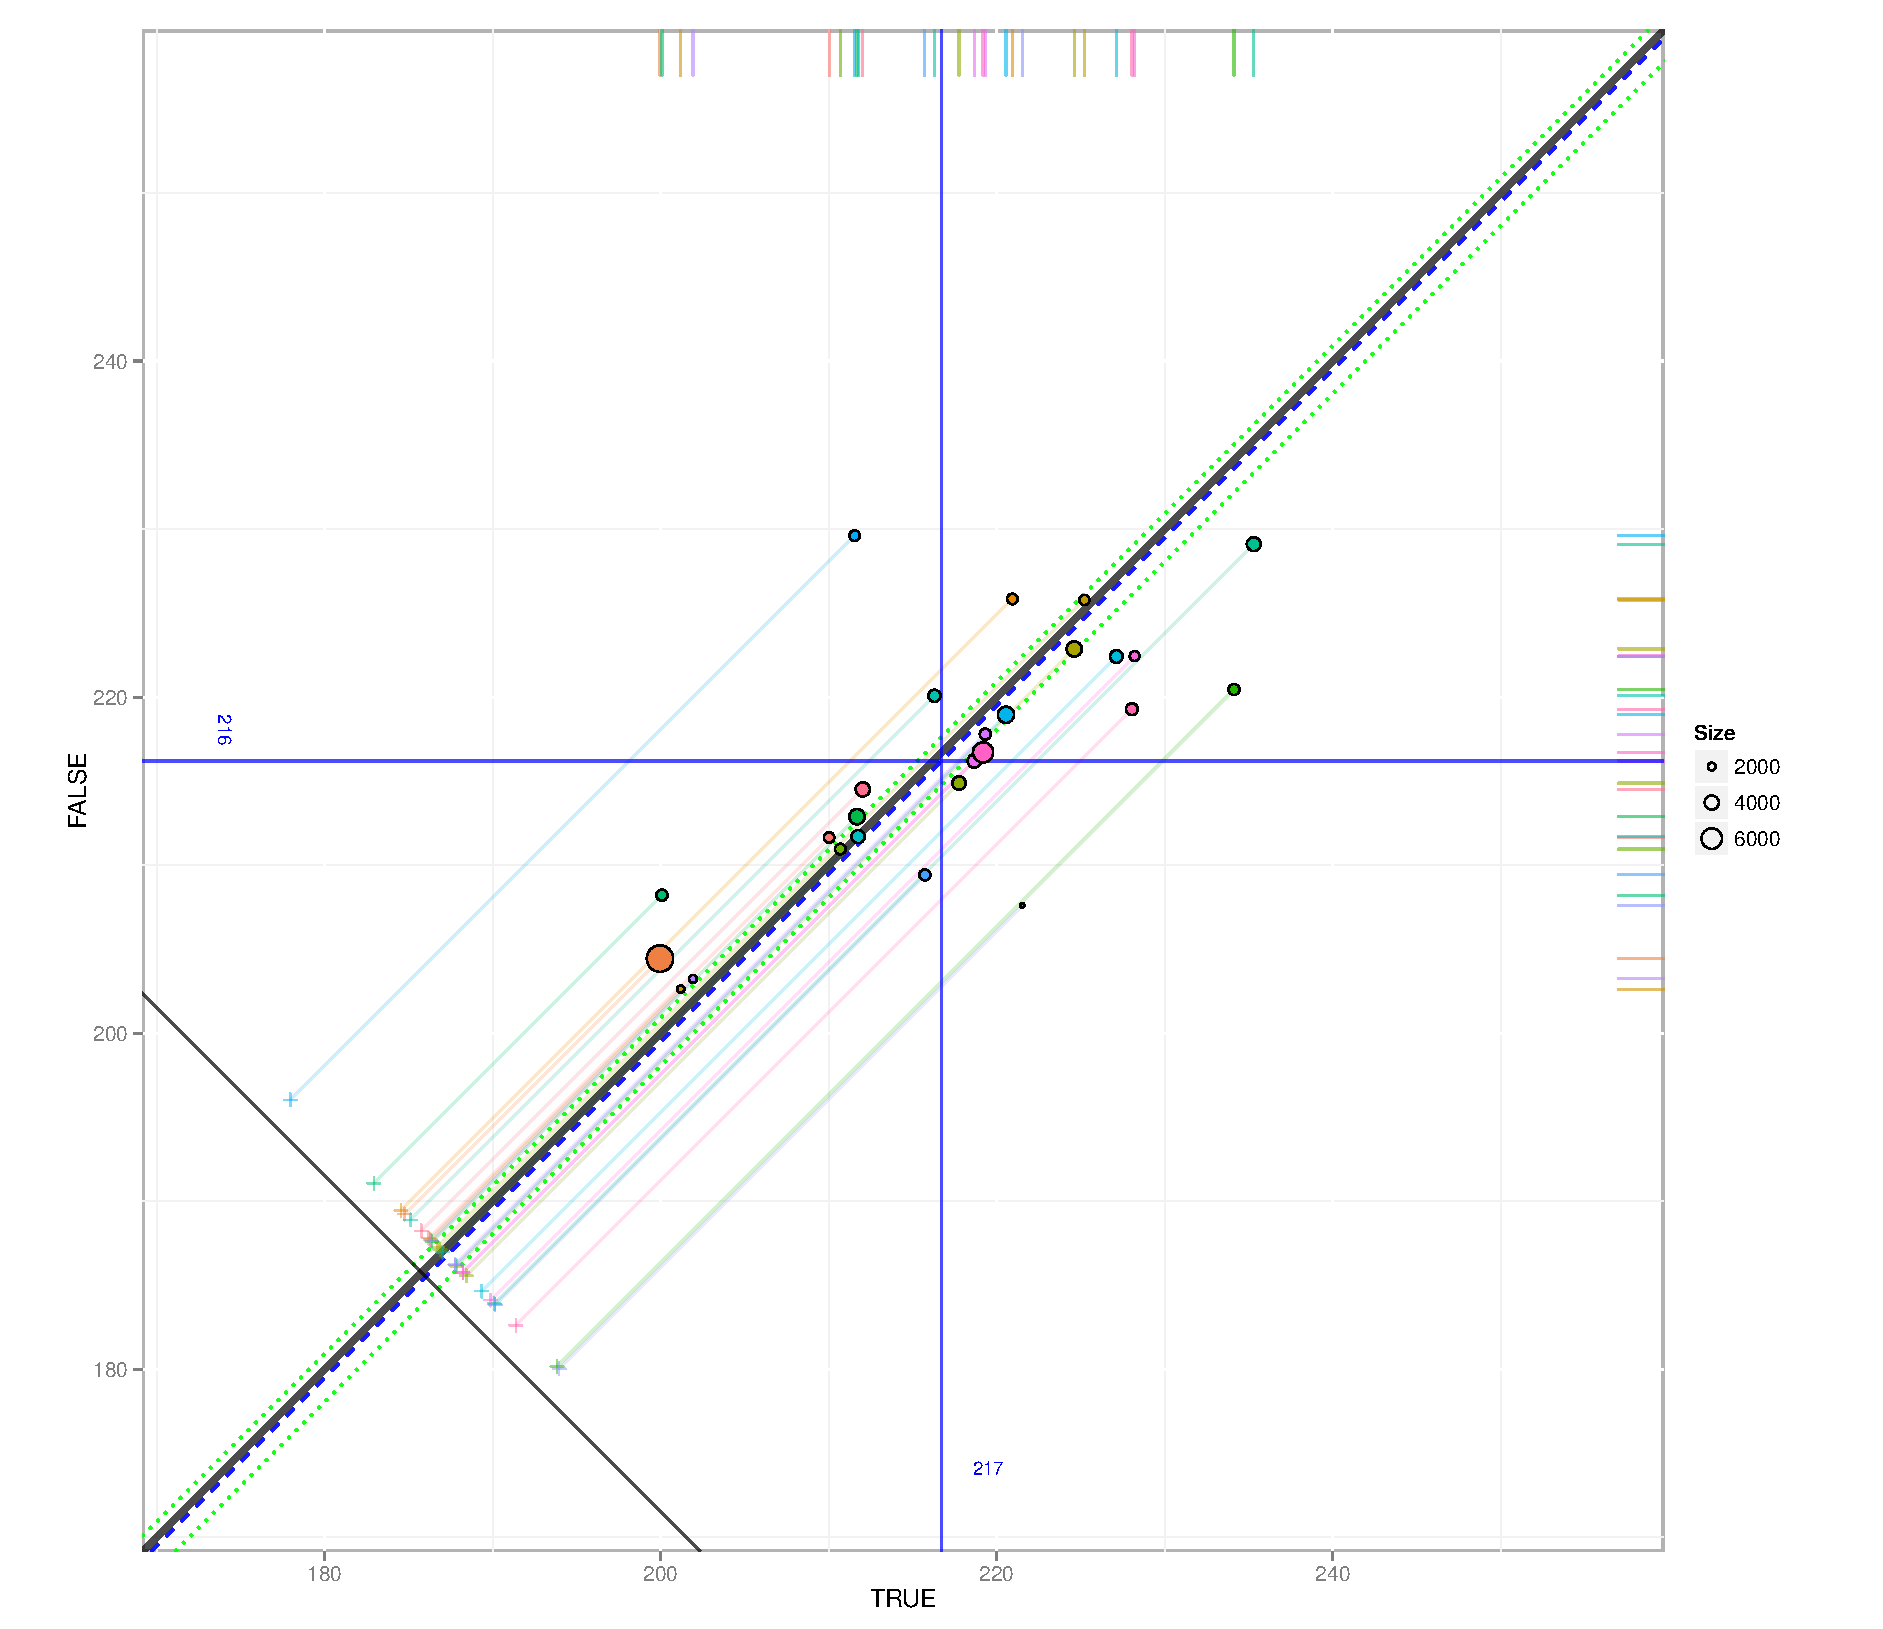
\includegraphics[width=\textwidth]{../Figures2009/g4read-mlpsa-ctree-circ.pdf}
\caption{Multilevel PSA assessment plot classification trees: Grade 4 reading}
\end{center}
\end{figure}

\begin{figure}[h!]
\begin{center}
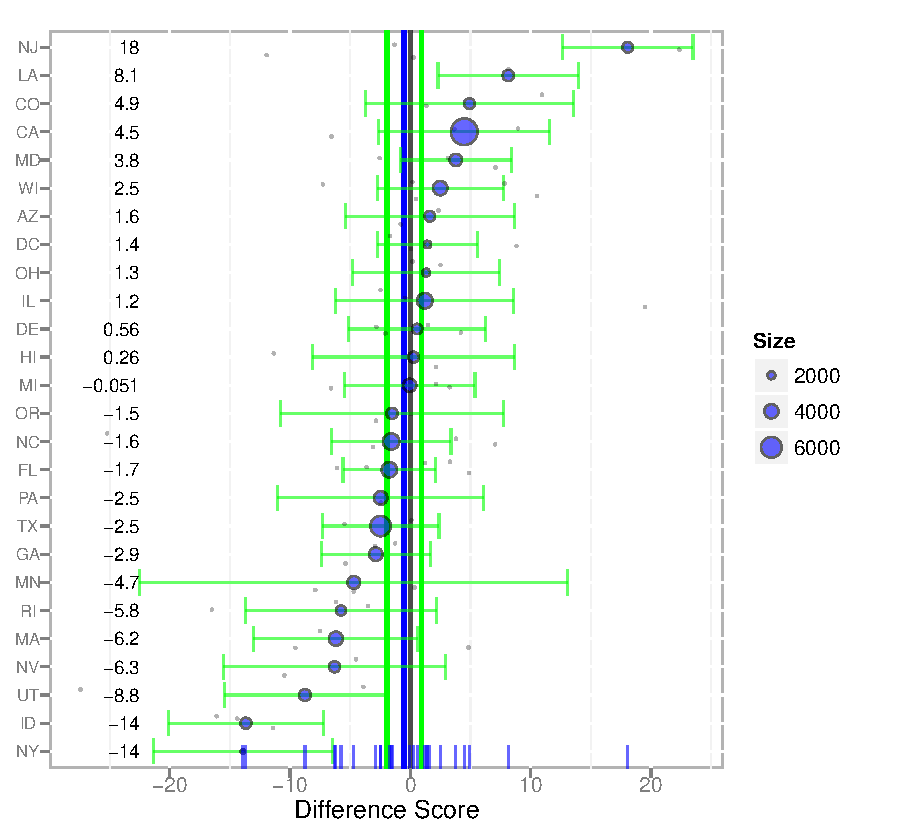
\includegraphics[width=\textwidth]{../Figures2009/g4read-mlpsa-ctree-diff.pdf}
\caption{Multilevel PSA difference plot classification trees: Grade 4 reading}
\end{center}
\label{fig:g4read-mlpsa-ctree-diff}
\end{figure}

% Grade 8 math
\begin{figure}[h!]
\begin{center}
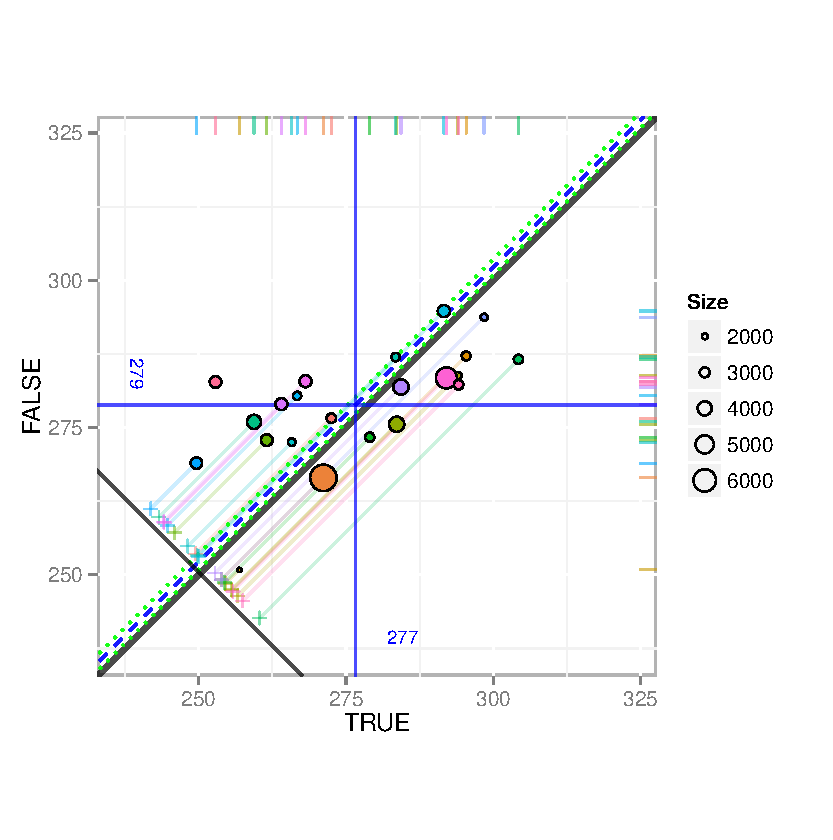
\includegraphics[width=\textwidth]{../Figures2009/g8math-mlpsa-lr-circ.pdf}
\caption{Multilevel PSA assessment plot logistic regression: Grade 8 math}
\end{center}
\end{figure}

\begin{figure}[h!]
\begin{center}
\includegraphics[width=\textwidth]{../Figures2009/g8math-mlpsa-lr-diff.pdf}
\caption{Multilevel PSA difference plot logistic regression: Grade 8 math}
\end{center}
\end{figure}

\begin{figure}[h!]
\begin{center}
\includegraphics[width=\textwidth]{../Figures2009/g8math-mlpsa-lrAIC-circ.pdf}
\caption{Multilevel PSA assessment plot logistic regression AIC: Grade 8 math}
\end{center}
\end{figure}

\begin{figure}[h!]
\begin{center}
\includegraphics[width=\textwidth]{../Figures2009/g8math-mlpsa-lrAIC-diff.pdf}
\caption{Multilevel PSA difference plot logistic regression AIC: Grade 8 math}
\end{center}
\end{figure}

\begin{figure}[h!]
\begin{center}
\includegraphics[width=\textwidth]{../Figures2009/g8math-mlpsa-ctree-circ.pdf}
\caption{Multilevel PSA assessment plot classification trees: Grade 8 math}
\end{center}
\end{figure}

\begin{figure}[h!]
\begin{center}
\includegraphics[width=\textwidth]{../Figures2009/g8math-mlpsa-ctree-diff.pdf}
\caption{Multilevel PSA difference plot classification trees: Grade 8 math}
\end{center}
\label{fig:g8math-mlpsa-ctree-diff}
\end{figure}

% Grade 8 reading
\begin{figure}[h!]
\begin{center}
\includegraphics[width=\textwidth]{../Figures2009/g8read-mlpsa-lr-circ.pdf}
\caption{Multilevel PSA assessment plot logistic regression: Grade 8 reading}
\end{center}
\end{figure}

\begin{figure}[h!]
\begin{center}
\includegraphics[width=\textwidth]{../Figures2009/g8read-mlpsa-lr-diff.pdf}
\caption{Multilevel PSA difference plot logistic regression: Grade 8 reading}
\end{center}
\end{figure}

\begin{figure}[h!]
\begin{center}
\includegraphics[width=\textwidth]{../Figures2009/g8read-mlpsa-lrAIC-circ.pdf}
\caption{Multilevel PSA assessment plot logistic regression AIC: Grade 8 reading}
\end{center}
\end{figure}

\begin{figure}[h!]
\begin{center}
\includegraphics[width=\textwidth]{../Figures2009/g8read-mlpsa-lrAIC-diff.pdf}
\caption{Multilevel PSA difference plot logistic regression AIC: Grade 8 reading}
\end{center}
\end{figure}

\begin{figure}[h!]
\begin{center}
\includegraphics[width=\textwidth]{../Figures2009/g8read-mlpsa-ctree-circ.pdf}
\caption{Multilevel PSA assessment plot classification trees: Grade 8 reading}
\end{center}
\end{figure}

\begin{figure}[h!]
\begin{center}
\includegraphics[width=\textwidth]{../Figures2009/g8read-mlpsa-ctree-diff.pdf}
\caption{Multilevel PSA difference plot classification trees: Grade 8 reading}
\end{center}
\label{fig:g8read-mlpsa-ctree-diff}
\end{figure}


%\begin{singlespace}
%% latex table generated in R 3.0.2 by xtable 1.7-1 package
% Sun Feb 23 12:16:13 2014
\begin{longtable}{lrrr@{\extracolsep{.25cm}}rrc}
\caption{Multilevel PSA Results using Conditional Inference Trees: Grade 4 math} \\ 
   \hline & & \multicolumn{2}{c}{FALSE} & \multicolumn{2}{c}{TRUE} & \\ \cline{3-4} \cline{5-6} Level & Strata & Mean & n & Mean & n & Confidence Interval \\ \hline\endfirsthead \multicolumn{7}{l}{{...continued from previous page}}\\ \hline  & & \multicolumn{2}{c}{FALSE} & \multicolumn{2}{c}{TRUE} & \\ \cline{3-4} \cline{5-6} Level & Strata & Mean & n & Mean & n & Confidence Interval \\ \hline \endhead \endfoot \endlastfoot  \hline
AZ & Overall & 229.05 & 2814 & 225.07 & 226 & ( -7.698, -0.25) \\ 
   & 1 & 220.30 & 1634 & 215.58 &  83 &  \\ 
   & 2 & 240.40 & 1180 & 237.40 & 143 &  \\ 
   \hline
CA & Overall & 227.08 & 7099 & 224.91 & 170 & ( -6.426,  2.09) \\ 
   & 1 & 215.33 & 574 & 224.84 &  36 &  \\ 
   & 2 & 233.93 & 3848 & 229.80 &  57 &  \\ 
   & 3 & 219.98 & 2677 & 218.00 &  77 &  \\ 
   \hline
CO & Overall & 242.63 & 2516 & 245.67 & 132 & ( -5.508, 11.59) \\ 
   & 1 & 252.17 & 1540 & 253.17 & 114 &  \\ 
   & 2 & 226.75 & 976 & 233.19 &  18 &  \\ 
   \hline
DC & Overall & 218.84 & 1282 & 219.35 & 512 & ( -3.388,  4.41) \\ 
   & 1 & 245.74 & 294 & 240.12 &  48 &  \\ 
   & 2 & 214.47 & 322 & 218.15 & 229 &  \\ 
   & 3 & 211.30 & 666 & 212.20 & 235 &  \\ 
   \hline
DE & Overall & 239.29 & 2499 & 241.24 & 195 & ( -3.280,  7.18) \\ 
   & 1 & 228.64 & 889 & 230.41 & 107 &  \\ 
   & 2 & 232.74 & 445 & 234.26 &   6 &  \\ 
   & 3 & 248.40 & 568 & 249.20 &  26 &  \\ 
   & 4 & 251.78 & 597 & 255.35 &  56 &  \\ 
   \hline
FL & Overall & 240.16 & 4273 & 238.74 & 166 & ( -5.046,  2.20) \\ 
   & 1 & 251.88 & 1294 & 247.59 &  58 &  \\ 
   & 2 & 247.21 & 390 & 245.49 &  39 &  \\ 
   & 3 & 233.06 & 2589 & 233.14 &  69 &  \\ 
   \hline
GA & Overall & 232.69 & 3811 & 239.31 & 164 & (  1.825, 11.43) \\ 
   & 1 & 253.95 & 147 & 261.10 &   5 &  \\ 
   & 2 & 233.67 & 350 & 236.84 &  20 &  \\ 
   & 3 & 255.04 & 968 & 255.75 &  60 &  \\ 
   & 4 & 221.72 & 2346 & 231.36 &  79 &  \\ 
   \hline
HI & Overall & 236.20 & 2642 & 230.95 &  57 & (-12.175,  1.67) \\ 
   & 1 & 236.20 & 2642 & 230.95 &  57 &  \\ 
   \hline
ID & Overall & 240.96 & 2807 & 252.03 &  60 & (  0.836, 21.31) \\ 
   & 1 & 227.12 & 773 & 240.20 &   5 &  \\ 
   & 2 & 246.11 & 2034 & 256.44 &  55 &  \\ 
   \hline
IL & Overall & 232.75 & 4047 & 239.45 &  78 & (  1.083, 12.32) \\ 
   & 1 & 213.59 & 1079 & 217.26 &  41 &  \\ 
   & 2 & 243.67 & 1772 & 252.94 &  10 &  \\ 
   & 3 & 234.38 & 1196 & 240.12 &  27 &  \\ 
   \hline
LA & Overall & 229.43 & 2789 & 230.80 &  65 & ( -2.790,  5.53) \\ 
   & 1 & 229.43 & 2789 & 230.80 &  65 &  \\ 
   \hline
MA & Overall & 238.41 & 1864 & 228.12 &  50 & (-16.052, -4.52) \\ 
   & 1 & 239.41 & 978 & 229.67 &  37 &  \\ 
   & 2 & 237.28 & 886 & 226.38 &  13 &  \\ 
   \hline
MD & Overall & 238.63 & 3195 & 237.80 & 141 & ( -5.527,  3.87) \\ 
   & 1 & 258.67 & 1181 & 270.72 &  10 &  \\ 
   & 2 & 234.72 & 528 & 229.66 &  18 &  \\ 
   & 3 & 222.11 & 790 & 210.48 &  85 &  \\ 
   & 4 & 233.49 & 379 & 227.17 &   7 &  \\ 
   & 5 & 222.97 & 317 & 217.82 &  21 &  \\ 
   \hline
MI & Overall & 225.51 & 2767 & 229.25 & 211 & ( -2.811, 10.28) \\ 
   & 1 & 230.22 & 633 & 235.66 &  18 &  \\ 
   & 2 & 215.93 & 175 & 229.48 &  26 &  \\ 
   & 3 & 204.06 & 981 & 210.80 & 144 &  \\ 
   & 4 & 248.95 & 969 & 246.30 &  18 &  \\ 
   & 5 & 216.47 &   9 & 207.70 &   5 &  \\ 
   \hline
MN & Overall & 248.30 & 2969 & 253.45 & 106 & (  0.237, 10.07) \\ 
   & 1 & 223.41 & 281 & 230.24 &  34 &  \\ 
   & 2 & 251.14 & 2688 & 256.10 &  72 &  \\ 
   \hline
NC & Overall & 243.63 & 4035 & 242.27 &  92 & ( -7.267,  4.55) \\ 
   & 1 & 254.56 & 1998 & 251.50 &  58 &  \\ 
   & 2 & 241.40 & 490 & 256.37 &  25 &  \\ 
   & 3 & 229.93 & 1547 & 225.42 &   9 &  \\ 
   \hline
NJ & Overall & 246.86 & 2747 & 235.10 &  74 & (-20.975, -2.55) \\ 
   & 1 & 250.18 & 2370 & 237.40 &  15 &  \\ 
   & 2 & 237.74 & 154 & 226.48 &   5 &  \\ 
   & 3 & 223.53 & 223 & 220.26 &  54 &  \\ 
   \hline
NV & Overall & 234.83 & 2784 & 231.01 &  72 & (-11.091,  3.46) \\ 
   & 1 & 234.83 & 2784 & 231.01 &  72 &  \\ 
   \hline
NY & Overall & 225.58 & 849 & 230.20 &  57 & ( -1.313, 10.54) \\ 
   & 1 & 225.58 & 849 & 230.20 &  57 &  \\ 
   \hline
OH & Overall & 215.58 & 1105 & 214.62 & 118 & (-11.058,  9.13) \\ 
   & 1 & 214.25 & 885 & 218.18 & 112 &  \\ 
   & 2 & 221.47 & 220 & 198.93 &   6 &  \\ 
   \hline
PA & Overall & 237.81 & 3460 & 237.31 &  50 & ( -7.521,  6.53) \\ 
   & 1 & 248.64 & 2165 & 239.34 &  15 &  \\ 
   & 2 & 223.28 & 329 & 235.48 &   8 &  \\ 
   & 3 & 218.70 & 751 & 231.20 &  13 &  \\ 
   & 4 & 219.85 & 215 & 241.04 &  14 &  \\ 
   \hline
RI & Overall & 238.67 & 2404 & 241.31 &  79 & ( -3.149,  8.43) \\ 
   & 1 & 246.32 & 1771 & 247.64 &  21 &  \\ 
   & 2 & 218.83 & 633 & 224.90 &  58 &  \\ 
   \hline
TX & Overall & 238.98 & 6162 & 230.83 &  91 & (-15.817, -0.48) \\ 
   & 1 & 235.46 & 3664 & 231.55 &  75 &  \\ 
   & 2 & 244.22 & 2498 & 229.77 &  16 &  \\ 
   \hline
UT & Overall & 239.88 & 2921 & 244.66 & 197 & ( -1.178, 10.73) \\ 
   & 1 & 219.92 & 673 & 228.28 &  20 &  \\ 
   & 2 & 245.59 & 2248 & 249.34 & 177 &  \\ 
   \hline
WI & Overall & 237.59 & 3637 & 242.59 & 136 & (  0.041,  9.96) \\ 
   & 1 & 248.66 & 2255 & 257.62 &  31 &  \\ 
   & 2 & 219.72 & 1119 & 217.56 &  67 &  \\ 
   & 3 & 226.36 &  46 & 228.04 &  17 &  \\ 
   & 4 & 223.30 & 217 & 226.81 &  21 &  \\ 
   \hline \multicolumn{7}{l}{\textit{Note:} Removed 7816 (10\%) rows due to insufficent data within a given strata.} \\\hline
\label{g4math-mlpsa-ctree}
\end{longtable}

%\clearpage
%% latex table generated in R 3.0.0 by xtable 1.7-1 package
% Thu May 30 09:15:19 2013
\begin{longtable}{lrrr@{\extracolsep{.25cm}}rrc}
\caption{Multilevel PSA Results using Conditional Inference Trees: Grade 4 read} \\ 
   \hline & & \multicolumn{2}{c}{TRUE} & \multicolumn{2}{c}{FALSE} & \\ \cline{3-4} \cline{5-6} Level & Strata & Mean & n & Mean & n & Confidence Interval \\ \hline\endfirsthead \multicolumn{7}{l}{{...continued from previous page}}\\ \hline  & & \multicolumn{2}{c}{TRUE} & \multicolumn{2}{c}{FALSE} & \\ \cline{3-4} \cline{5-6} Level & Strata & Mean & n & Mean & n & Confidence Interval \\ \hline \endhead \endfoot \endlastfoot  \hline
AZ & Overall & 210.03 & 240 & 211.64 & 2640 & ( -5.42,  8.65) \\ 
   & 1 & 216.79 & 208 & 219.13 & 2007 &  \\ 
   & 2 & 187.50 &  32 & 186.70 & 633 &  \\ 
   \hline
CA & Overall & 199.96 & 183 & 204.44 & 7659 & ( -2.63, 11.59) \\ 
   & 1 & 216.07 &  26 & 225.03 & 2463 &  \\ 
   & 2 & 190.72 & 123 & 194.38 & 4570 &  \\ 
   & 3 & 204.92 &  34 & 198.37 & 626 &  \\ 
   \hline
CO & Overall & 220.93 & 143 & 225.84 & 2742 & ( -3.75, 13.57) \\ 
   & 1 & 236.36 & 120 & 237.69 & 1692 &  \\ 
   & 2 & 194.89 &  23 & 205.83 & 1050 &  \\ 
   \hline
DC & Overall & 201.20 & 541 & 202.62 & 1307 & ( -2.72,  5.56) \\ 
   & 1 & 220.08 &  48 & 228.91 & 336 &  \\ 
   & 2 & 193.93 & 296 & 194.00 & 674 &  \\ 
   & 3 & 200.79 & 197 & 199.12 & 297 &  \\ 
   \hline
DE & Overall & 225.22 & 216 & 225.78 & 2557 & ( -5.15,  6.28) \\ 
   & 1 & 235.52 &  92 & 237.00 & 1106 &  \\ 
   & 2 & 221.95 &  11 & 219.88 & 594 &  \\ 
   & 3 & 209.15 &  80 & 213.35 & 459 &  \\ 
   & 4 & 221.27 &  33 & 218.46 & 398 &  \\ 
   \hline
FL & Overall & 224.61 & 183 & 222.87 & 4168 & ( -5.60,  2.10) \\ 
   & 1 & 217.18 &  21 & 213.55 & 1290 &  \\ 
   & 2 & 224.15 &  48 & 218.04 & 1356 &  \\ 
   & 3 & 226.57 &  33 & 227.79 & 377 &  \\ 
   & 4 & 234.03 &  19 & 237.33 & 461 &  \\ 
   & 5 & 231.42 &  62 & 236.31 & 684 &  \\ 
   \hline
GA & Overall & 217.76 & 173 & 214.89 & 3606 & ( -7.39,  1.64) \\ 
   & 1 & 237.09 &  48 & 231.69 & 974 &  \\ 
   & 2 & 201.14 &  30 & 198.20 & 1074 &  \\ 
   & 3 & 216.90 &  95 & 215.65 & 1558 &  \\ 
   \hline
HI & Overall & 210.69 &  78 & 210.96 & 2855 & ( -8.11,  8.64) \\ 
   & 1 & 237.23 &  22 & 225.88 & 382 &  \\ 
   & 2 & 206.46 &  56 & 208.57 & 2473 &  \\ 
   \hline
ID & Overall & 234.12 &  72 & 220.45 & 2931 & (-20.11, -7.23) \\ 
   & 1 & 239.78 &  25 & 223.67 & 984 &  \\ 
   & 2 & 248.74 &  38 & 234.36 & 650 &  \\ 
   & 3 & 222.06 &   9 & 210.64 & 1297 &  \\ 
   \hline
IL & Overall & 211.68 &  81 & 212.89 & 4301 & ( -6.19,  8.60) \\ 
   & 1 & 195.88 &  42 & 193.39 & 751 &  \\ 
   & 2 & 180.14 &   6 & 199.66 & 433 &  \\ 
   & 3 & 220.06 &  33 & 219.64 & 3117 &  \\ 
   \hline
LA & Overall & 200.08 &  73 & 208.21 & 3039 & (  2.30, 13.98) \\ 
   & 1 & 200.08 &  73 & 208.21 & 3039 &  \\ 
   \hline
MA & Overall & 235.30 &  54 & 229.11 & 3883 & (-13.01,  0.62) \\ 
   & 1 & 247.44 &   5 & 239.91 & 2154 &  \\ 
   & 2 & 208.52 &   9 & 213.34 & 607 &  \\ 
   & 3 & 226.94 &  40 & 217.39 & 1122 &  \\ 
   \hline
MD & Overall & 216.30 & 152 & 220.08 & 3246 & ( -0.84,  8.40) \\ 
   & 1 & 227.01 &  31 & 234.09 & 1692 &  \\ 
   & 2 & 214.52 &  36 & 211.98 & 774 &  \\ 
   & 3 & 196.61 &  85 & 199.75 & 780 &  \\ 
   \hline
MI & Overall & 211.75 & 213 & 211.70 & 3462 & ( -5.47,  5.37) \\ 
   & 1 & 222.09 &  30 & 225.35 & 1998 &  \\ 
   & 2 & 207.26 &  33 & 209.37 & 434 &  \\ 
   & 3 & 195.76 & 150 & 189.16 & 1030 &  \\ 
   \hline
MN & Overall & 227.12 & 109 & 222.42 & 3427 & (-22.49, 13.09) \\ 
   & 1 & 220.53 &   6 & 220.86 & 206 &  \\ 
   & 2 & 201.32 &  33 & 193.41 & 295 &  \\ 
   & 3 & 230.41 &  70 & 225.71 & 2926 &  \\ 
   \hline
NC & Overall & 220.55 & 104 & 218.95 & 4559 & ( -6.57,  3.37) \\ 
   & 1 & 219.75 &  28 & 223.55 & 575 &  \\ 
   & 2 & 230.21 &  30 & 237.26 & 1642 &  \\ 
   & 3 & 204.01 &  16 & 200.93 & 1731 &  \\ 
   & 4 & 241.19 &  30 & 215.99 & 611 &  \\ 
   \hline
NJ & Overall & 211.54 &  80 & 229.61 & 2764 & ( 12.64, 23.49) \\ 
   & 1 & 218.87 &  15 & 219.13 & 190 &  \\ 
   & 2 & 215.48 &  24 & 203.54 & 145 &  \\ 
   & 3 & 210.99 &  26 & 209.67 &  53 &  \\ 
   & 4 & 210.65 &  15 & 233.01 & 2376 &  \\ 
   \hline
NV & Overall & 215.72 &  75 & 209.42 & 2947 & (-15.54,  2.93) \\ 
   & 1 & 218.29 &  11 & 207.81 & 892 &  \\ 
   & 2 & 214.63 &  64 & 210.11 & 2055 &  \\ 
   \hline
NY & Overall & 221.53 &  68 & 207.60 & 876 & (-21.36, -6.49) \\ 
   & 1 & 221.53 &  68 & 207.60 & 876 &  \\ 
   \hline
OH & Overall & 201.92 & 136 & 203.24 & 1888 & ( -4.80,  7.42) \\ 
   & 1 & 209.00 &  11 & 211.51 & 978 &  \\ 
   & 2 & 195.16 & 125 & 195.33 & 910 &  \\ 
   \hline
OR & Overall & 219.32 &  56 & 217.80 & 3001 & (-10.78,  7.73) \\ 
   & 1 & 232.36 &  42 & 229.50 & 1619 &  \\ 
   & 2 & 203.81 &  14 & 203.87 & 1382 &  \\ 
   \hline
PA & Overall & 218.66 &  59 & 216.20 & 3713 & (-11.03,  6.11) \\ 
   & 1 & 218.66 &  59 & 216.20 & 3713 &  \\ 
   \hline
RI & Overall & 228.21 &  85 & 222.44 & 2566 & (-13.73,  2.20) \\ 
   & 1 & 234.09 &  21 & 230.58 & 1886 &  \\ 
   & 2 & 213.83 &  14 & 197.33 & 373 &  \\ 
   & 3 & 212.39 &  50 & 206.22 & 307 &  \\ 
   \hline
TX & Overall & 219.19 & 100 & 216.71 & 5827 & ( -7.33,  2.37) \\ 
   & 1 & 214.70 &  66 & 209.22 & 2658 &  \\ 
   & 2 & 223.01 &  34 & 223.09 & 3169 &  \\ 
   \hline
UT & Overall & 228.05 & 203 & 219.29 & 3057 & (-15.45, -2.07) \\ 
   & 1 & 225.05 &  13 & 197.63 & 660 &  \\ 
   & 2 & 228.83 & 190 & 224.92 & 2397 &  \\ 
   \hline
WI & Overall & 212.03 & 153 & 214.51 & 3878 & ( -2.75,  7.71) \\ 
   & 1 & 225.61 &  43 & 225.79 & 2468 &  \\ 
   & 2 & 180.75 &  48 & 188.57 & 545 &  \\ 
   & 3 & 193.65 &  25 & 204.17 & 601 &  \\ 
   & 4 & 202.04 &  17 & 202.49 &  48 &  \\ 
   & 5 & 197.65 &  20 & 190.38 & 216 &  \\ 
   \hline \multicolumn{7}{l}{\textit{Note:} Removed 5874 (6\%) rows due to insufficent data within a given strata.} \\\hline
\label{g4read-mlpsa-ctree}
\end{longtable}

%\clearpage
%% latex table generated in R 3.0.1 by xtable 1.7-1 package
% Tue Jun 11 08:07:12 2013
\begin{longtable}{lrrr@{\extracolsep{.25cm}}rrc}
\caption{Multilevel PSA Results using Conditional Inference Trees: Grade 8 math} \\ 
   \hline & & \multicolumn{2}{c}{FALSE} & \multicolumn{2}{c}{TRUE} & \\ \cline{3-4} \cline{5-6} Level & Strata & Mean & n & Mean & n & Confidence Interval \\ \hline\endfirsthead \multicolumn{7}{l}{{...continued from previous page}}\\ \hline  & & \multicolumn{2}{c}{FALSE} & \multicolumn{2}{c}{TRUE} & \\ \cline{3-4} \cline{5-6} Level & Strata & Mean & n & Mean & n & Confidence Interval \\ \hline \endhead \endfoot \endlastfoot  \hline
AZ & Overall & 276.44 & 2788 & 268.79 & 105 & (-17.602,   2.3) \\ 
   & 1 & 291.73 & 1394 & 272.25 &  19 &  \\ 
   & 2 & 260.02 & 1256 & 262.21 &  61 &  \\ 
   & 3 & 272.99 & 112 & 285.37 &   9 &  \\ 
   & 4 & 286.72 &  26 & 310.59 &  16 &  \\ 
   \hline
CA & Overall & 266.36 & 6459 & 271.98 & 525 & (  2.706,   8.5) \\ 
   & 1 & 271.35 & 2292 & 278.30 & 130 &  \\ 
   & 2 & 234.05 & 937 & 239.70 &  85 &  \\ 
   & 3 & 266.32 & 2409 & 271.25 & 250 &  \\ 
   & 4 & 290.26 & 821 & 294.29 &  60 &  \\ 
   \hline
CO & Overall & 287.36 & 2604 & 286.97 & 125 & ( -8.464,   7.7) \\ 
   & 1 & 267.84 & 851 & 252.01 &  22 &  \\ 
   & 2 & 296.54 & 1753 & 303.42 & 103 &  \\ 
   \hline
DC & Overall & 249.96 & 818 & 257.47 & 825 & (  2.577,  12.5) \\ 
   & 1 & 235.15 &  58 & 252.17 &  27 &  \\ 
   & 2 & 234.66 &  79 & 257.21 &  80 &  \\ 
   & 3 & 242.24 & 299 & 251.99 & 350 &  \\ 
   & 4 & 286.75 & 142 & 277.06 &  70 &  \\ 
   & 5 & 255.90 & 166 & 260.06 & 260 &  \\ 
   & 6 & 232.20 &  38 & 241.79 &  30 &  \\ 
   & 7 & 240.26 &  36 & 254.41 &   8 &  \\ 
   \hline
DE & Overall & 283.99 & 2275 & 290.37 & 201 & (  1.611,  11.1) \\ 
   & 1 & 279.59 & 1475 & 282.79 &  91 &  \\ 
   & 2 & 291.56 & 800 & 303.40 & 110 &  \\ 
   \hline
FL & Overall & 275.86 & 4012 & 280.59 & 272 & ( -0.078,   9.5) \\ 
   & 1 & 274.38 & 393 & 272.11 &  13 &  \\ 
   & 2 & 296.24 & 860 & 292.32 &  82 &  \\ 
   & 3 & 281.43 & 486 & 286.07 &  74 &  \\ 
   & 4 & 265.25 & 841 & 281.50 &  25 &  \\ 
   & 5 & 267.57 & 1432 & 273.00 &  78 &  \\ 
   \hline
GA & Overall & 263.18 & 2110 & 260.09 &  88 & (-10.868,   4.7) \\ 
   & 1 & 260.45 & 309 & 269.04 &  24 &  \\ 
   & 2 & 263.67 & 1801 & 258.49 &  64 &  \\ 
   \hline
HI & Overall & 273.61 & 2652 & 274.30 & 167 & ( -7.142,   8.5) \\ 
   & 1 & 267.90 & 105 & 256.78 &   5 &  \\ 
   & 2 & 285.84 & 273 & 292.77 &  50 &  \\ 
   & 3 & 266.45 & 1114 & 271.12 &  38 &  \\ 
   & 4 & 277.60 & 1160 & 273.99 &  74 &  \\ 
   \hline
ID & Overall & 293.06 & 1963 & 301.86 &  90 & (  1.983,  15.6) \\ 
   & 1 & 284.39 & 923 & 295.55 &  34 &  \\ 
   & 2 & 302.38 & 938 & 307.40 &  43 &  \\ 
   & 3 & 285.64 & 102 & 307.11 &  13 &  \\ 
   \hline
IL & Overall & 275.66 & 3897 & 269.00 & 110 & (-24.036,  10.7) \\ 
   & 1 & 260.89 & 2105 & 261.65 & 104 &  \\ 
   & 2 & 293.80 & 1792 & 278.03 &   6 &  \\ 
   \hline
IN & Overall & 286.56 & 2546 & 302.77 &  77 & (  8.810,  23.6) \\ 
   & 1 & 278.54 &  67 & 279.22 &  18 &  \\ 
   & 2 & 256.38 &  10 & 285.35 &  10 &  \\ 
   & 3 & 260.33 & 183 & 259.80 &  23 &  \\ 
   & 4 & 275.56 & 169 & 303.71 &   7 &  \\ 
   & 5 & 290.60 & 2117 & 307.93 &  19 &  \\ 
   \hline
LA & Overall & 272.53 & 2359 & 266.23 &  90 & (-13.079,   0.5) \\ 
   & 1 & 272.53 & 2359 & 266.23 &  90 &  \\ 
   \hline
MA & Overall & 294.76 & 3476 & 293.08 &  61 & ( -9.212,   5.8) \\ 
   & 1 & 291.70 & 1284 & 291.86 &   7 &  \\ 
   & 2 & 303.25 & 1476 & 298.17 &  28 &  \\ 
   & 3 & 282.89 & 716 & 284.89 &  26 &  \\ 
   \hline
MD & Overall & 282.19 & 2881 & 264.30 &  72 & (-25.666, -10.1) \\ 
   & 1 & 295.51 & 1816 & 263.47 &   9 &  \\ 
   & 2 & 260.63 & 1065 & 265.65 &  63 &  \\ 
   \hline
MI & Overall & 268.17 & 3206 & 260.58 & 160 & (-13.917,  -1.3) \\ 
   & 1 & 286.30 & 1954 & 271.50 &  34 &  \\ 
   & 2 & 242.02 & 1252 & 244.84 & 126 &  \\ 
   \hline
MN & Overall & 294.58 & 2655 & 295.27 &  80 & ( -7.845,   9.2) \\ 
   & 1 & 287.93 & 1556 & 285.83 &  18 &  \\ 
   & 2 & 308.66 & 987 & 313.60 &  45 &  \\ 
   & 3 & 263.16 & 112 & 263.83 &  17 &  \\ 
   \hline
NC & Overall & 281.95 & 4235 & 287.15 &  93 & ( -1.789,  12.2) \\ 
   & 1 & 255.14 & 170 & 232.76 &  12 &  \\ 
   & 2 & 266.64 & 1576 & 277.75 &  15 &  \\ 
   & 3 & 293.39 & 2489 & 296.87 &  66 &  \\ 
   \hline
OH & Overall & 278.88 & 3389 & 267.60 &  94 & (-17.227,  -5.3) \\ 
   & 1 & 283.22 & 2639 & 271.14 &  55 &  \\ 
   & 2 & 264.08 & 750 & 255.49 &  39 &  \\ 
   \hline
PA & Overall & 285.47 & 3192 & 277.46 & 109 & (-14.452,  -1.6) \\ 
   & 1 & 267.28 & 218 & 249.42 &  23 &  \\ 
   & 2 & 241.63 &  38 & 251.54 &  15 &  \\ 
   & 3 & 289.52 & 2764 & 281.15 &  54 &  \\ 
   & 4 & 260.52 & 172 & 265.35 &  17 &  \\ 
   \hline
TX & Overall & 283.52 & 5562 & 288.70 & 134 & ( -6.564,  16.9) \\ 
   & 1 & 287.92 & 4756 & 292.02 & 129 &  \\ 
   & 2 & 257.02 & 806 & 268.72 &   5 &  \\ 
   \hline
UT & Overall & 282.76 & 2681 & 292.19 & 110 & (  1.275,  17.6) \\ 
   & 1 & 282.11 & 1254 & 288.18 &  44 &  \\ 
   & 2 & 296.83 & 932 & 299.94 &  55 &  \\ 
   & 3 & 256.99 & 495 & 287.35 &  11 &  \\ 
   \hline
WI & Overall & 281.76 & 3182 & 264.85 & 231 & (-22.636, -11.2) \\ 
   & 1 & 299.57 & 1404 & 277.44 &  18 &  \\ 
   & 2 & 278.65 & 323 & 274.25 &  13 &  \\ 
   & 3 & 272.08 &  79 & 250.45 &  13 &  \\ 
   & 4 & 266.40 & 178 & 249.34 &  76 &  \\ 
   & 5 & 256.63 & 783 & 244.80 &  92 &  \\ 
   & 6 & 287.48 & 415 & 268.85 &  19 &  \\ 
   \hline \multicolumn{7}{l}{\textit{Note:} Removed 2600 (4\%) rows due to insufficent data within a given strata.} \\\hline
\label{g8math-mlpsa-ctree}
\end{longtable}

%\clearpage
%% latex table generated in R 3.0.1 by xtable 1.7-1 package
% Tue Jun 11 08:07:49 2013
\begin{longtable}{lrrr@{\extracolsep{.25cm}}rrc}
\caption{Multilevel PSA Results using Conditional Inference Trees: Grade 8 read} \\ 
   \hline & & \multicolumn{2}{c}{FALSE} & \multicolumn{2}{c}{TRUE} & \\ \cline{3-4} \cline{5-6} Level & Strata & Mean & n & Mean & n & Confidence Interval \\ \hline\endfirsthead \multicolumn{7}{l}{{...continued from previous page}}\\ \hline  & & \multicolumn{2}{c}{FALSE} & \multicolumn{2}{c}{TRUE} & \\ \cline{3-4} \cline{5-6} Level & Strata & Mean & n & Mean & n & Confidence Interval \\ \hline \endhead \endfoot \endlastfoot  \hline
AZ & Overall & 257.47 & 2680 & 261.71 &  92 & ( -6.904, 15.37) \\ 
   & 1 & 258.74 & 2361 & 262.02 &  65 &  \\ 
   & 2 & 251.15 & 306 & 262.71 &  18 &  \\ 
   & 3 & 210.84 &  13 & 211.83 &   9 &  \\ 
   \hline
CA & Overall & 247.26 & 6536 & 254.93 & 500 & (  4.973, 10.38) \\ 
   & 1 & 206.68 & 947 & 212.97 & 102 &  \\ 
   & 2 & 219.00 & 361 & 226.51 &  63 &  \\ 
   & 3 & 260.14 & 1178 & 271.89 &  45 &  \\ 
   & 4 & 270.44 & 956 & 275.94 &  61 &  \\ 
   & 5 & 247.90 & 1554 & 257.79 &  83 &  \\ 
   & 6 & 255.65 & 1540 & 260.44 & 146 &  \\ 
   \hline
CO & Overall & 264.41 & 2607 & 273.13 & 148 & (  4.021, 13.41) \\ 
   & 1 & 273.27 & 995 & 286.26 &  51 &  \\ 
   & 2 & 271.98 & 631 & 275.01 &  72 &  \\ 
   & 3 & 249.91 & 981 & 258.15 &  25 &  \\ 
   \hline
DC & Overall & 240.03 & 780 & 245.92 & 792 & ( -0.046, 11.83) \\ 
   & 1 & 236.24 & 399 & 245.16 & 445 &  \\ 
   & 2 & 230.53 & 224 & 239.42 & 156 &  \\ 
   & 3 & 250.11 &  21 & 244.28 &  33 &  \\ 
   & 4 & 297.63 &  55 & 278.73 &  15 &  \\ 
   & 5 & 249.99 &  81 & 249.99 & 143 &  \\ 
   \hline
DE & Overall & 264.73 & 2301 & 273.72 & 195 & (  4.388, 13.59) \\ 
   & 1 & 264.10 & 795 & 263.32 &  65 &  \\ 
   & 2 & 271.95 & 437 & 278.61 &  71 &  \\ 
   & 3 & 257.43 & 562 & 282.47 &  17 &  \\ 
   & 4 & 266.74 & 507 & 276.25 &  42 &  \\ 
   \hline
FL & Overall & 262.04 & 3883 & 268.60 & 281 & (  2.895, 10.22) \\ 
   & 1 & 256.79 & 1184 & 265.62 &  54 &  \\ 
   & 2 & 267.59 & 992 & 271.57 &  57 &  \\ 
   & 3 & 262.41 & 1707 & 268.91 & 170 &  \\ 
   \hline
GA & Overall & 258.28 & 3314 & 254.85 &  86 & (-13.986,  7.13) \\ 
   & 1 & 272.06 & 1474 & 265.06 &  11 &  \\ 
   & 2 & 248.00 & 1805 & 247.78 &  69 &  \\ 
   & 3 & 228.87 &  35 & 208.28 &   6 &  \\ 
   \hline
HI & Overall & 254.50 & 2693 & 251.88 & 172 & ( -7.888,  2.65) \\ 
   & 1 & 247.01 & 1575 & 243.23 &  69 &  \\ 
   & 2 & 268.19 & 683 & 268.50 &  79 &  \\ 
   & 3 & 258.58 & 435 & 255.26 &  24 &  \\ 
   \hline
ID & Overall & 264.05 & 2721 & 280.43 &  86 & ( 10.231, 22.53) \\ 
   & 1 & 254.71 & 1463 & 275.68 &  16 &  \\ 
   & 2 & 260.54 & 265 & 266.56 &  13 &  \\ 
   & 3 & 278.13 & 993 & 290.79 &  57 &  \\ 
   \hline
IL & Overall & 248.65 & 2228 & 249.43 & 102 & ( -4.449,  6.02) \\ 
   & 1 & 243.48 & 1064 & 247.00 &  69 &  \\ 
   & 2 & 253.54 & 1164 & 251.74 &  33 &  \\ 
   \hline
IN & Overall & 266.29 & 2554 & 260.93 &  77 & (-10.384, -0.33) \\ 
   & 1 & 268.49 & 2285 & 262.73 &  24 &  \\ 
   & 2 & 260.56 &  69 & 252.88 &  28 &  \\ 
   & 3 & 246.14 & 200 & 245.90 &  25 &  \\ 
   \hline
LA & Overall & 253.37 & 2374 & 250.34 &  89 & ( -8.927,  2.86) \\ 
   & 1 & 253.37 & 2374 & 250.34 &  89 &  \\ 
   \hline
MA & Overall & 269.76 & 3493 & 282.53 &  53 & (  4.911, 20.63) \\ 
   & 1 & 261.54 & 804 & 260.39 &  27 &  \\ 
   & 2 & 268.46 & 1760 & 286.93 &   9 &  \\ 
   & 3 & 279.41 & 929 & 293.75 &  17 &  \\ 
   \hline
MD & Overall & 246.30 & 1435 & 250.32 &  76 & ( -1.022,  9.07) \\ 
   & 1 & 249.79 & 1064 & 253.72 &  37 &  \\ 
   & 2 & 236.90 & 371 & 241.19 &  39 &  \\ 
   \hline
MI & Overall & 255.03 & 3155 & 256.46 & 162 & ( -4.285,  7.13) \\ 
   & 1 & 236.39 & 1224 & 237.56 & 125 &  \\ 
   & 2 & 267.81 & 1931 & 269.40 &  37 &  \\ 
   \hline
MN & Overall & 269.37 & 2710 & 274.13 &  78 & ( -2.784, 12.31) \\ 
   & 1 & 249.83 & 286 & 232.18 &  18 &  \\ 
   & 2 & 268.76 & 2040 & 276.67 &  31 &  \\ 
   & 3 & 286.81 & 384 & 292.31 &  29 &  \\ 
   \hline
NC & Overall & 258.13 & 4269 & 259.41 &  90 & ( -6.023,  8.59) \\ 
   & 1 & 252.16 & 2445 & 244.24 &  33 &  \\ 
   & 2 & 266.00 & 1824 & 279.39 &  57 &  \\ 
   \hline
OH & Overall & 262.97 & 3260 & 253.77 &  87 & (-15.357, -3.03) \\ 
   & 1 & 266.02 & 2544 & 254.84 &  55 &  \\ 
   & 2 & 252.37 & 716 & 250.06 &  32 &  \\ 
   \hline
PA & Overall & 263.48 & 3220 & 269.89 & 117 & (  1.242, 11.57) \\ 
   & 1 & 275.14 & 2254 & 281.11 &  33 &  \\ 
   & 2 & 241.16 & 247 & 244.00 &  18 &  \\ 
   & 3 & 232.88 & 443 & 246.19 &  25 &  \\ 
   & 4 & 243.24 & 276 & 245.54 &  41 &  \\ 
   \hline
RI & Overall & 257.86 & 2444 & 268.04 &  46 & (  0.850, 19.50) \\ 
   & 1 & 237.30 & 494 & 250.48 &  19 &  \\ 
   & 2 & 244.48 & 159 & 262.18 &  22 &  \\ 
   & 3 & 265.08 & 1791 & 273.64 &   5 &  \\ 
   \hline
TX & Overall & 257.71 & 5521 & 260.45 & 131 & ( -3.093,  8.58) \\ 
   & 1 & 254.33 & 3926 & 254.10 &  59 &  \\ 
   & 2 & 265.79 & 1595 & 275.65 &  72 &  \\ 
   \hline
UT & Overall & 263.69 & 2712 & 272.35 & 118 & (  3.596, 13.71) \\ 
   & 1 & 255.00 & 1538 & 264.44 &  43 &  \\ 
   & 2 & 274.69 & 1174 & 282.36 &  75 &  \\ 
   \hline
WI & Overall & 262.00 & 3131 & 255.63 & 216 & (-11.049, -1.68) \\ 
   & 1 & 244.61 & 965 & 238.63 & 156 &  \\ 
   & 2 & 270.75 & 2166 & 264.19 &  60 &  \\ 
   \hline \multicolumn{7}{l}{\textit{Note:} Removed 3807 (5\%) rows due to insufficent data within a given strata.} \\\hline
\label{g8read-mlpsa-ctree}
\end{longtable}

%\end{singlespace}



%==================== Appendix I ====================================================================
\clearpage
\addcontentsline{toc}{subsection}{Appendix I: Multilevel PSA Classification Tree Heat Maps}
\section*{Appendix I\\Multilevel PSA Classification Tree Heat Maps}
\label{appendixI}

\begin{figure}[h!]
\begin{center}
\includegraphics[height=.37\textheight]{../Figures2009/g4math-mlpsa-ctree-heat.pdf}
\caption{Heat map of relative importance of covariates from classification trees: Grade 4 math}
\label{fig:g4math-mlpsa-ctree-heat}
\end{center}
\end{figure}

\begin{figure}[h!]
\begin{center}
\includegraphics[height=.37\textheight]{../Figures2009/g4read-mlpsa-ctree-heat.pdf}
\caption{Heat map of relative importance of covariates from classification trees: Grade 4 reading}
\label{fig:g4read-mlpsa-ctree-heat}
\end{center}
\end{figure}

\begin{figure}[h!]
\begin{center}
\includegraphics[height=.37\textheight]{../Figures2009/g8math-mlpsa-ctree-heat.pdf}
\caption{Heat map of relative importance of covariates from classification trees: Grade 8 math}
\label{fig:g8math-mlpsa-ctree-heat}
\end{center}
\end{figure}

\begin{figure}[h!]
\begin{center}
\includegraphics[height=.37\textheight]{../Figures2009/g8read-mlpsa-ctree-heat.pdf}
\caption{Heat map of relative importance of covariates from classification trees: Grade 8 reading}
\label{fig:g8read-mlpsa-ctree-heat}
\end{center}
\end{figure}


%==================== Appendix J ====================================================================
\clearpage
\addcontentsline{toc}{subsection}{Appendix J: multilevelPSA R Package}
\section*{Appendix J\\multilevelPSA R Package}
\label{appendixJ}

The \texttt{multilevelPSA} R package was developed, in part, to conduct the analysis for this dissertation. It is available from the Comprehensive R Archive Network (CRAN) at \url{http://cran.r-project.org/web/packages/multilevelPSA}. The latest version can be installed using the \texttt{install.packages} function in R:

\begin{verbatim}
> install.packages('multilevelPSA', repos='http://cran.r-project.org')
\end{verbatim}

The following list provides brief descriptions of the key functions in the \texttt{multilevelPSA} package. More information is available vis-\`a-vis the R help system.

\renewcommand{\descriptionlabel}[1]{\hspace{\labelsep}\textbf{\texttt{#1}}}
\begin{description}
\item[getPropensityScores] Returns a data frame with two columns corresponding to the level 2 variable and the fitted value from the logistic regression.
\item[getStrata] Returns a data frame with two columns corresponding to the level 2 variable and the leaves from the conditional inference trees.
\item[loess.plot] Loess plot with density distributions for propensity scores and outcomes on top and right, respectively.
\item[missing.plot] Returns a heat map graphic representing missingness of variables grouped by the given grouping vector.
\item[mlpsa] This function will perform phase II of the multilevel propensity score analysis.
\item[plot.mlpsa] Creates the multilevel assessment plot.
\item[mlpsa.circ.plot] Plots the results of a multilevel propensity score model.
\item[mlpsa.ctree] Estimates propensity scores using the recursive partitioning in a conditional inference framework.
\item[mlpsa.difference.plot] Creates a graphic summarizing the differences between treatment and comparison groups within and across level two clusters.
\item[mlpsa.distribution.plot] Plots distribution for either the treatment or comparison group.
\item[mlpsa.logistic] Estimates propensity scores using logistic regression.
\item[psrange] Estimates models with increasing number of comparison subjects starting from 1:1 to using all available comparison group subjects.
\item[plot.psrange] Plots the results of \texttt{psrange}.
\item[tree.plot] Heat map representing variables used in a conditional inference tree across level 2 variables.
\end{description}

%==================== Appendix K ====================================================================
\clearpage
\addcontentsline{toc}{subsection}{Appendix K: Simulating Propensity Score Ranges}
\section*{Appendix K\\Simulating Propensity Score Ranges}
\label{appendixK}

\begin{singlespace}

\noindent The \texttt{getSimulatedData} function is what is used to simulate covariates with varying overlap.

\begin{verbatim}
getSimulatedData <- function(nvars = 3, 
    ntreat = 100, treat.mean = 0.6, treat.sd = 0.5, 
    ncontrol = 1000, control.mean = 0.4, control.sd = 0.5) {
    if (length(treat.mean) == 1) {
        treat.mean = rep(treat.mean, nvars)
    }
    if (length(treat.sd) == 1) {
        treat.sd = rep(treat.sd, nvars)
    }
    if (length(control.mean) == 1) {
        control.mean = rep(control.mean, nvars)
    }
    if (length(control.sd) == 1) {
        control.sd = rep(control.sd, nvars)
    }
    
    df <- c(rep(0, ncontrol), rep(1, ntreat))
    for (i in 1:nvars) {
        df <- cbind(df, c(
            rnorm(ncontrol, mean = control.mean[1], sd = control.sd[1]), 
            rnorm(ntreat, mean = treat.mean[1], sd = treat.sd[1])
        ) )
    }
    df <- as.data.frame(df)
    names(df) <- c("treat", letters[1:nvars])
    return(df)
}
\end{verbatim}

\noindent The following code was used to create Figure \ref{fig:psranges} in Chapter 5 which represents moderate overlap but some separation in covariates between treatment and control.


\begin{verbatim}
set.seed(2112)
df.psrange <- getSimulatedData(ncontrol = 1000, nvars=1,
                               treat.mean=0.6, treat.sd=0.4,
                               control.mean=0.4, control.sd=0.4)
psrange.test <- psrange(df.psrange, df.psrange$treat, treat ~ ., 
                        samples = seq(100, 1000, by = 100), nboot = 20)
plot(psrange.test)
\end{verbatim}

\noindent The following simulates covariates with perfect overlap (i.e. the differences between covariate values between treatment and control is random).

\begin{verbatim}
df.overlap <- getSimulatedData(ncontrol = 1000, nvars=1,
                               treat.mean=0.5, treat.sd=0.4,
                               control.mean=0.5, control.sd=0.4)
psrange.overlap <- psrange(df.overlap, df.overlap$treat, treat ~ ., 
                           samples = seq(100, 1000, by = 100), nboot = 20)
plot(psrange.overlap)
\end{verbatim}

\begin{figure}[h!]
\begin{center}
\includegraphics[width=\textwidth]{../Figures2009/PSRanges-Overlap.pdf}
\caption{Propensity score ranges for varying treatment-to-control ratios with perfect overlapping covariate}
\end{center}
\end{figure}

\noindent The following simulates covariates with almost no overlap (i.e. the covariate values can almost perfectly predict treatment placement).

\begin{verbatim}
df.nooverlap <- getSimulatedData(ncontrol = 1000, nvars=1,
                                 treat.mean=0.2, treat.sd=0.4,
                                 control.mean=0.8, control.sd=0.4)
psrange.nooverlap <- psrange(df.nooverlap, df.nooverlap$treat, treat ~ ., 
                             samples = seq(100, 1000, by = 100), nboot = 20)
plot(psrange.nooverlap)
\end{verbatim}

\begin{figure}[h!]
\begin{center}
\includegraphics[width=\textwidth]{../Figures2009/PSRanges-NoOverlap.pdf}
\caption{Propensity score ranges for varying treatment-to-control ratios with non-overlapping covariate}
\end{center}
\end{figure}

\end{singlespace}


%==================== Appendix L ====================================================================
\clearpage
\addcontentsline{toc}{subsection}{Appendix L: Rubric for Rating the Quality of Charter School Laws}
\section*{Appendix L\\Rubric for Rating the Quality of Charter School Laws}
\label{appendixL}

This appendix contains the rubric used by the \citeA{NAPCS2010a} to rate the quality of state charter laws. For each state law rated, the law is given a score between 0 to 4 for each of the 20 components. The score for each component is then multiplied by the weight (ranging from 1 to 4) and those 20 values are summed to provide a total score. The range of possible scores for each law therefore ranges between 0 and 208.

\begin{singlespace}
\begin{landscape}
% latex table generated in R 3.1.1 by xtable 1.7-3 package
% Sun Aug 31 21:12:47 2014
{\smaller
\begin{longtable}{rp{2.2in}p{0.9in}p{0.9in}p{0.9in}p{0.9in}p{0.9in}c}
\caption{NAPCS Rubric for Rating the Quality of State Charter Laws} \\ 
   \hline & & \multicolumn{5}{c}{Scoring} & \\ \cline{3-7}& Component & \multicolumn{1}{c}{0} & \multicolumn{1}{c}{1} & \multicolumn{1}{c}{2} & \multicolumn{1}{c}{3} & \multicolumn{1}{c}{4} & Weight \\ \hline\endfirsthead \multicolumn{8}{l}{{...continued from previous page}}\\ \hline & & \multicolumn{5}{c}{Scoring} & \\ \cline{3-7}& Component & \multicolumn{1}{c}{0} & \multicolumn{1}{c}{1} & \multicolumn{1}{c}{2} & \multicolumn{1}{c}{3} & \multicolumn{1}{c}{4} & Weight \\ \hline \endhead   1 & No Caps, whereby: 1A. No limits are placed on the number of public charter schools or students (and no geographic limits). 1B. If caps exist, adequate room for growth.  & The state has a cap with no room for growth.  & The state has a cap with room for limited growth.  & The state has a cap with room for some growth.  & The state has a cap with room for ample growth. OR The state does not have a cap, but allows districts to restrict growth.  & The state does not have a cap. &   3 \\ 
   \hline
  2 & A Variety of Public Charter Schools Allowed, including: 2A. New start-ups. 2B. Public school conversions. 2C. Virtual schools.  & The state allows only public school conversions.  & Not Applicable  & The state allows new start-ups and public school conversions, but not virtual schools. OR The state allows only new start-ups.  & The state allows new start-ups and virtual schools, but not public school conversions.  & The state allows new start-ups, public school conversions, and virtual schools.  &   1 \\ 
   \hline
  3 & Multiple Authorizers Available, including: 3A. Two or more viable authorizing options for each applicant with direct application allowed to each authorizing option.  & The state has only a single viable authorizer option available, and there is no or almost no authorizing activity.  & The state has only a single viable authorizer option available, and there is some authorizing activity.  & The state has only a single viable authorizer option available, and there is considerable authorizing activity. OR The state allows two or more viable authorizing options for applicants in some but not all situations.  & The state allows two or more viable authorizing options for each applicant, but requires applicants to get preliminary approval from a state charter school advisory committee.  & The state allows two or more viable authorizing options for each applicant.  &   3 \\ 
   \hline \pagebreak \hline
  4 & Authorizer and Overall Program Accountability System Required, including: 4A. At least a registration process for local school boards to affirm their interest in chartering to the state. 4B. Application process for other eligible authorizing entities. 4C. Authorizer submission of annual report, which summarizes the agency’s authorizing activities as well as the performance of its school portfolio. 4D. A regular review process by authorizer oversight body. 4E. Authorizer oversight body with authority to sanction authorizers, including removal of authorizer right to approve schools. 4F. Periodic formal evaluation of overall state charter school program and outcomes.  & The state law includes none of the elements of the model law’s authorizer and overall program accountability system.  & The state law includes a small number of the elements of the model law’s authorizer and overall program accountability system.  & The state law includes some of the elements of the model law’s authorizer and overall program accountability system.  & The state law includes many of the elements of the model law’s authorizer and overall program accountability system.  & The state law includes all of the elements of the model law’s authorizer and overall program accountability system.  &   3 \\ 
   \hline
  5 & Adequate Authorizer Funding, including: 5A. Adequate funding from authorizing fees (or other sources). 5B. Guaranteed funding from authorizing fees (or from sources not subject to annual legislative appropriations). 5E. Prohibition on authorizers requiring schools to purchase services from them.  & The state law includes none of the model law’s provisions for adequate authorizer funding.  & The state law includes a small number of the model law’s provisions for adequate authorizer funding.  & The state law includes some of the model law’s provisions for adequate authorizer funding.  & The state law includes many of the model law’s provisions for adequate authorizer funding.  & The state law includes all of the model law’s provisions for adequate authorizer funding.  &   2 \\ 
   \hline
  6 & Transparent Charter Application, Review, and Decision-making Processes, including: 6A. Application elements for all schools. 6B. Additional application elements specific to conversion schools. 6C. Additional application elements specific to virtual schools. 6D. Additional application elements specific when using educational service providers. 6E. Additional application elements specific to replications. 6F. Authorizer-issued request for proposals (including application requirements and approval criteria). 6G. Thorough evaluation of each application including an in-person interview and a public meeting. 6H. All charter approval or denial decisions made in a public meeting, with authorizers stating reasons for denials in writing.  & The state law includes none of the model law’s provisions for transparent charter application, review, and decision- making processes.  & The state law includes a small number of the model law’s provisions for transparent charter application, review, and decision-making processes.  & The state law includes some of the model law’s provisions for transparent charter application, review, and decision-making processes.  & The state law includes many of the model law’s provisions for transparent charter application, review, and decision-making processes.  & The state law includes all of the model law’s provisions for transparent charter application, review, and decision- making processes.  &   4 \\ 
   \hline
  7 & Performance-Based Charter Contracts Required, with such contracts: 7A. Being created as a separate document from the application and executed by the governing board of the charter school and the authorizer. 7B. Defining the roles, powers, and responsibilities for the school and its authorizer. 7C. Defining academic and operational performance expectations by which the school will be judged, based on a performance framework that includes measures and metrics for, at a minimum, student academic proficiency and growth, achievement gaps, attendance, recurrent enrollment, postsecondary readiness (high schools), financial performance, and board stewardship (including compliance). 7D. Providing an initial term of five operating years (or a longer term with periodic high-stakes reviews). 7E. Including requirements addressing the unique environments of virtual schools, if applicable.  & The state law includes none of the model law’s provisions for performance- based charter contracts.  & The state law includes a small number of the model law’s provisions for performance- based charter contracts.  & The state law includes some of the model law’s provisions for performance- based charter contracts.  & The state law includes many of the model law’s provisions for performance- based charter contracts.  & The state law includes all of the model law’s provisions for performance- based charter contracts.  &   4 \\ 
   \hline
  8 & Comprehensive Charter School Monitoring and Data Collection Processes, including: 8A. The collection and analysis of student outcome data at least annually by authorizers (consistent with performance framework outlined in the contract). 8B. Financial accountability for charter schools (e.g., Generally Accepted Accounting Principles, independent annual audit reported to authorizer). 8C. Authorizer authority to conduct or require oversight activities. 8D. Annual school performance reports produced and made public by each authorizer. 8E. Authorizer notification to their schools of perceived problems, with opportunities to remedy such problems. 8F. Authorizer authority to take appropriate corrective actions or exercise sanctions short of revocation. & The state law includes none of the model law’s provisions for comprehensive charter school monitoring and data collection processes.  & The state law includes a small number of the model law’s provisions for comprehensive charter school monitoring and data collection processes.  & The state law includes some of the model law’s provisions for comprehensive charter school monitoring and data collection processes.  & The state law includes many of the model law’s provisions for comprehensive charter school monitoring and data collection processes.  & The state law includes all of the model law’s provisions for comprehensive charter school monitoring and data collection processes.  &   4 \\ 
   \hline
  9 & Clear Processes for Renewal, Nonrenewal, and Revocation Decisions, including: 9A. Authorizer must issue school performance renewal reports to schools whose charter will expire the following year. 9B. Schools seeking renewal must apply for it. 9C. Authorizers must issue renewal application guidance that provides an opportunity for schools to augment their performance record and discuss improvements and future plans. 9D. Clear criteria for renewal and nonrenewal/revocation. 9E. Authorizers must ground renewal decisions based on evidence regarding the school’s performance over the term of the charter contract (in accordance with the performance framework set forth in the charter contract). 9F. Authorizer authority to vary length of charter renewal contract terms based on performance or other issues. 9G. Authorizers must provide charter schools with timely notification of potential revocation or non-renewal (including reasons) and reasonable time to respond. 9H. Authorizers must provide charter schools with due process for nonrenewal and revocation decisions (e.g., public hearing, submission of evidence). 9I. All charter renewal, non-renewal, and revocation decisions made in a public meeting, with authorizers stating reasons for non-renewals and revocations in writing. 9J. Authorizers must have school closure protocols to ensure timely parent notification, orderly student and record transitions, and property and asset disposition.  & The state law includes none of the model law’s clear processes for renewal, nonrenewal, and revocation decisions.  & The state law includes a small number of the model law’s clear processes for renewal, nonrenewal, and revocation decisions.  & The state law includes some of the model law’s clear processes for renewal, nonrenewal, and revocation decisions.  & The state law includes many of the model law’s clear processes for renewal, nonrenewal, and revocation decisions.  & The state law includes all of the model law’s clear processes for renewal, nonrenewal, and revocation decisions.  &   4 \\ 
   \hline
 10 & Educational Service Providers Allowed, including: 10A. All types of educational service providers allowed to operate all or parts of charter schools. 10A. All types of educational service providers allowed to operate all or parts of charter schools. 10B. A performance contract between the independent public charter school board and the service provider is required. 10C. Existing and potential conflicts of interest between the two entities are required to be disclosed and explained in application.  & The state law prohibits charter schools from contracting with all types of educational service providers.  & The state law is silent regarding these arrangements. OR The state law prohibits contracting with certain types of educational service providers.  & The state law explicitly allows contracting with all types of educational service providers but does not include provisions regarding performance contracts and conflicts of interest.  & The state law explicitly allows contracting with all types of educational service providers and requires performance contracts or conflicts of interest provisions, but not both.  & The state law explicitly allows contracting with all types of educational service providers and has provisions regarding performance contracts and conflicts of interest.  &   2 \\ 
   \hline
 11 & Fiscally and Legally Autonomous Schools with Independent Public Charter School Boards, including: 11A. Fiscally and legally autonomous schools (e.g., schools have authority to receive and disburse funds, enter into contracts, and sue and be sued in their own names). 11B. School governing boards independent of the authorizer and created specifically to govern their charter school(s).  & The state law includes none of the model law’s provisions for fiscally and legally autonomous schools with independent public charter school boards.  & The state law includes a small number of the model law’s provisions for fiscally and legally autonomous schools with independent public charter school boards.  & The state law includes some of the model law’s provisions for fiscally and legally autonomous schools with independent public charter school boards. OR
The state law includes all of these provisions for some schools, but not others. & The state law includes many of the model law’s provisions for fiscally and legally autonomous schools with independent public charter school boards.  & The state law includes all of the model law’s provisions for fiscally of the model law’s provisions for fiscally and legally autonomous schools with independent public charter school boards.  &   3 \\ 
   \hline
 12 & Clear Student Recruitment, Enrollment, and Lottery Procedures, including: 12A. Open enrollment to any student in the state. 12B. Lottery requirements. 12C. Required enrollment preferences for previously enrolled students within conversions, prior year students within chartered schools, and siblings of enrolled students enrolled at a charter school. 12D. Optional enrollment preference for children of a school’s founders, governing board members, and full-time employees, not exceeding 10\% of the school’s total student population. & The state law includes none (or nearly none) of the model law’s requirements for student recruitment, enrollment, and lottery procedures.  & The state law includes a small number of the model law’s requirements for student recruitment, enrollment, and lottery procedures.  & The state law includes some of the model law’s requirements for student recruitment, enrollment, and lottery procedures.  & The state law includes many of the model law’s requirements for student recruitment, enrollment, and lottery procedures.  & The state law includes all of the model law’s requirements for student recruitment, enrollment, and lottery procedures.  &   1 \\ 
   \hline
 13 & Automatic Exemptions from Many State and District Laws and Regulations, including: 13A. Exemptions from all laws, except those covering health, safety, civil rights, student accountability, employee criminal history checks, open meetings, freedom of information, and generally accepted accounting principles. 13B. Exemption from state teacher certification requirements.  & The state law does not provide automatic exemptions from state and district laws and regulations, does not allow schools to apply for exemptions, and requires all of a school’s teachers to be certified.  & The state law allows schools to apply for exemptions from state and district laws and requires all of a school’s teachers to be certified. OR The state law does not provide automatic exemptions from many state and district laws and regulations and does not require any of a school’s teachers to be certified. OR The state law allows schools to apply for exemptions from state and district laws and requires some of a school’s teachers to be certified. & There were six variations for how state laws handled 13A and 13B that were included in this cell.  & The state law provides automatic exemptions from many state and district laws and regulations and requires some of a school’s teachers to be certified.  & The state law provides automatic exemptions from many state and district laws and regulations and does not require any of a school’s teachers to be certified.  &   3 \\ 
   \hline
 14 & Automatic Collective Bargaining Exemption, whereby: 14A. Charter schools authorized by non-local board authorizers are exempt from participation in district collective bargaining agreements. 14B. Charter schools authorized by local boards are exempt from participation in district collective bargaining agreements.  & The state law requires all charter schools to be part of district collective bargaining agreements, with no opportunity for exemptions.  & The state law requires all charter schools to be part of district collective bargaining agreements, but schools can apply for exemptions.  & The state law exempts some schools from district collective bargaining agreements, but not others.  & The state law exempts some schools from district collective bargaining agreements, but not others (but allows those not exempted to apply for exemptions).  & The state law does not require any charter schools to be part of district collective bargaining agreements.  &   3 \\ 
   \hline
 15 & Multi-School Charter Contracts and/or Multi-Charter Contract Boards Allowed, whereby an independent public charter school board may: 15A. Oversee multiple schools linked under a single contract with independent fiscal and academic accountability for each school. 15B. Hold multiple charter contracts with independent fiscal and academic accountability for each school.  & The state law prohibits these arrangements.  & The state law is silent regarding these arrangements. OR
The state law explicitly allows either of these arrangements but does not require each school to be independently accountable for fiscal and academic performance. OR The state law explicitly allows these arrangements for some schools but not others.  & The state law allows either of these arrangements, but only requires schools authorized by some entities to be independently accountable for fiscal and academic performance.  & Not Applicable  & The state law explicitly allows either of these arrangements and requires each school to be independently accountable for fiscal and academic performance.  &   1 \\ 
   \hline
 16 & Extra-Curricular and Interscholastic Activities Eligibility and Access, whereby: 16A. Laws or regulations explicitly state that charter school students and employees are eligible to participate in all interscholastic leagues, competitions, awards, scholarships, and recognition programs available to non-charter public school students and employees. 16B. Laws or regulations explicitly allow charter school students in schools not providing extra-curricular and interscholastic activities to have access to those activities at non-charter public schools for a fee by a mutual agreement.  & The state law prohibits charter eligibility and access.  & The state law is silent about charter eligibility and access.  & The state law provides either charter eligibility or access, but not both.  & The state law provides both charter eligibility and access to students, but not employees.  & The state law provides both charter eligibility and access.  &   1 \\ 
   \hline
 17 & Clear Identification of Special Education Responsibilities, including: 17A. Clarity regarding which entity is the local education agency (LEA) responsible for providing special education services. 17B. Clarity regarding funding for low-incident, high-cost services for charter schools (in the same amount and/or in a manner similar to other LEAs).  & The state law is silent about special education responsibilities and funding for low-incident, high-cost services.  & The state law addresses special education, but is unclear about responsibility for providing services and funding for low-incident, high-cost services.  & The state law is clear on either responsibility for providing services OR funding for low-incident, high-cost services, but not both.  & Not Applicable  & The state law clearly addresses responsibility for providing services and ensures state funding for low-incident, high-cost services.  &   2 \\ 
   \hline
 18 & Equitable Operational Funding and Equal Access to All State and Federal Categorical Funding, including: 18A. Equitable operational funding statutorily driven.18B. Equal access to all applicable categorical federal and state funding, and clear guidance on the pass-through of such funds. 18C. Funding for transportation similar to school districts.  & The state law includes none of the model law’s provisions for equitable operational funding and equal access to all state and federal categorical funding.  & The state law includes a small number of the model law’s provisions for equitable operational funding and equal access to all state and federal categorical funding.  & The state law includes some of the model law’s provisions for equitable operational funding and equal access to all state and federal categorical funding.  & The state law includes many of the model law’s provisions for equitable operational funding and equal access to all state and federal categorical funding.  & The state law includes all of the model law’s provisions for equitable operational funding and equal access to all state and federal categorical funding.  &   3 \\ 
   \hline
 19 & Equitable Access to Capital Funding and Facilities, including: 19A. A per-pupil facilities allowance which annually reflects actual average district capital costs. 19B. A state grant program for charter school facilities. 19C. A state loan program for charter school facilities. 19D. Equal access to tax-exempt bonding authorities or allow charter schools to have their own bonding authority. 19E. A mechanism to provide credit enhancement for public charter school facilities. 19F. Equal access to existing state facilities programs available to non-charter public schools. 19G. Right of first refusal to purchase or lease at or below fair market value a closed, unused, or underused public school facility or property. 19H. Prohibition of facility-related requirements stricter than those applied to traditional public schools.  & The state law includes none of the model law’s provisions for equitable access to capital funding and facilities.  & The state law includes a small number of the model law’s provisions for equitable access to capital funding and facilities.  & The state law includes some of the model law’s provisions for equitable access to capital funding and facilities.  & The state law includes many of the model law’s provisions for equitable access to capital funding and facilities.  & The state law includes all of the model law’s provisions for equitable access to capital funding and facilities.  &   3 \\ 
   \hline
 20 & Automatic Collective Bargaining Exemption, whereby: 20A. Charter schools have access to relevant state retirement systems available to other public schools.  20B. Charter schools have the option to participate (i.e., not required).  & The state law does not provide access to the relevant employee retirement systems.  & The state law requires participation in the relevant employee retirement systems for some schools, but denies access to these systems for other schools.  & The state law requires participation in the relevant employee retirement systems.  & The state law provides that charter schools have access and an option by virtue of how they hire their employees. OR The state law requires participation in the relevant employee retirement systems, unless at the time of application, a school has a retirement program which covers the employees or the employee is currently enrolled in another retirement program. OR The state law provides some charter schools with the option to participate in the relevant state employee retirement systems, but not others. & The state law provides access to relevant employee retirement systems, but does not require participation.  &   3 \\ 
   \hline
\hline
\label{NAPCSrubric}
\end{longtable}
}

\end{landscape}
\end{singlespace}

%==================== Appendix M ====================================================================
%\clearpage
\addcontentsline{toc}{subsection}{Appendix M: Matrix Plot of NAPCS Charter Law Scores and NAEP Charter School Effect Sizes}
\section*{Appendix M\\Matrix Plot of NAPCS Charter Law Scores and NAEP Charter School Effect Sizes}
\label{appendixM}

\begin{figure}[h!]
\begin{center}
\includegraphics[width=\textwidth]{../Figures2009/NAEPLawScoresMatrixPlot.pdf}
\caption{Matrix plot of NAPCS charter law scores and NAEP charter school effect sizes}
\end{center}
\end{figure}



%%%%% Left Overs %%%%%%%%%%%%%%%%%%%%%%%%%%%%%%%%%%%%%%%%%%%%%%%%%%%%
%%%%% Themeatic Map

%\newpage
%\addcontentsline{toc}{subsection}{Appendix B: Thematic Map of Number of Charter Schools in the United States}
%\subsection*{Appendix B\\Thematic Map of Number of Charter Schools by State in 2008}
%\label{appendixMap}
%\begin{figure}[h]
%\includegraphics[width=\textwidth]{../Figures/CharterMap.pdf}
%\caption{Thematic map of number of charter schools by state in 2008}
%\label{fig:charterMap}
%\end{figure}

